
\documentclass[10pt,twocolumn,letterpaper]{article}

\usepackage[pagenumbers]{cvpr}              %

\usepackage{graphicx}
\usepackage{amsmath}
\usepackage{amssymb}
\usepackage{booktabs}
\usepackage{pifont}
\usepackage{caption}
\usepackage{subcaption}


\makeatletter
\@namedef{ver@everyshi.sty}{}
\makeatother
\usepackage{tikz}
\usepackage{pgfplots}
\usepackage{wrapfig}

\usepackage[accsupp]{axessibility}

\usepackage{algorithm}
\usepackage{algcompatible}
\usepackage{algorithmicx}
\usepackage{algpseudocode}


\usepackage{mathtools, cuted}
\usepackage{resizegather}

\usepackage{widetext}







\usepackage{rotating}
\usepackage{xr}







\usepackage[pagebackref,breaklinks,colorlinks]{hyperref}

\usepackage[capitalize]{cleveref}
\crefname{section}{Sec.}{Secs.}
\Crefname{section}{Section}{Sections}
\Crefname{table}{Table}{Tables}
\crefname{table}{Tab.}{Tabs.}


\usepackage{color} 
\definecolor{darkorange}{rgb}{1.0, 0.55, 0.0} 
\definecolor{darkgreen}{rgb}{0.0, 0.55, 0.0} 

\newcommand{\exy}[1]{\textcolor{darkorange}{#1}} 
\newcommand{\exz}[1]{\textcolor{darkgreen}{#1}} 
\newcommand{\eyz}[1]{\textcolor{blue}{#1}} 

\DeclareMathOperator*{\argmin}{arg\,min}


\begin{document}

\title{CCuantuMM: Cycle-Consistent Quantum-Hybrid Matching of Multiple Shapes} 

\author{Harshil Bhatia$^{1,2}$~~~Edith Tretschk$^2$~~~Zorah Lähner$^3$~~~Marcel Seelbach Benkner$^3$\\
Michael Moeller$^3$~~~Christian Theobalt$^2$~~~Vladislav Golyanik$^2$\\
$^1$Indian Institute of Technology, Jodhpur~~~~$^2$MPI for Informatics, SIC~~~~$^3$Universität Siegen
}
\maketitle

\begin{abstract}
   \begin{abstract}
The current study investigated possible human-robot kinaesthetic interaction using a variational recurrent neural network model, called PV-RNN, which is based on the free energy principle.
Our prior robotic studies using PV-RNN showed that the nature of interactions between top-down expectation and bottom-up inference is strongly affected by a parameter, called the meta-prior, which regulates the complexity term in free energy.
% The current study examines how the behaviours of robots alter by changing the meta-prior $w$ in human-robot kinaesthetic interaction.
The current study examines how changing the meta-prior $w$ in the interaction phase affects the counter force generated when an experimenter attempts to induce movement pattern transitions familiar to the robot through its prior training.
The study also compares the counter force generated when trained transitions are induced by a human experimenter and when untrained transitions are induced.
Our experimental results indicated that (1) the human experimenter needs more/less force to induce trained transitions when $w$ is set with larger/smaller values, (2) the human experimenter needs more force to act on the robot when he attempts to induce untrained as opposed to trained movement pattern transitions.
Our analysis of time development of essential variables and values in PV-RNN during bodily interaction clarified the mechanism by which gaps in actional intentions between the human experimenter and the robot can be manifested as reaction forces between them.


%% Hiroki writing 2022-11-4
%Current study investigates the dynamics of the latent states during human-robot kinaesthetic interaction using PV-RNN.
%We have achieved to observe and analyse the internal state of an RNN model based on the free energy principle, during real-time human-robot interaction.
%Essential characteristics observed in the previous study of this variational recurrent neural network model, PV-RNN, is that by changing a meta prior $w$, the balance between the top-down intention and the bottom-up perceptual reality changes.
%In the current study, we examined how changing the weighting parameter $w$ between accuracy and complexity in free energy principle affects the humanoid robot's behaviour through human-robot interaction. We have conducted some human-robot kinaesthetic interaction experiments with various $w$ and quantitatively analysed the latent variable and the force applied to the humanoid robot. We have observed that the force required to change the robot's intention has increased, both when the top-down intention was strengthened by changing the $w$ and when corresponding switch of its primitive was against the experience of the RNN during its training. The study confirms through quantitative analysis that by increasing or decreasing the $w$ in PV-RNN, humanoid robot leads or follows the human counterpart during the human-robot kinaesthetic interaction.

\begin{comment}
Comment from Jun #2
・最後にQualitativeな結果(インパクト)が欲しい
・Current study investigates the problem on~と書き出すのが一般的
・最初の一文と最後の一文を対応させる
・最後の一文はもう少しAbstractかつ包括的に
\end{comment}

\begin{comment}
Comment from Jun #1
We investigated how the kinaesthetic human-robot interaction can affect the internal state of a model based on the free energy principle. 
=> how the internal state is affected is not the most important point in this study. This part should be rewritten.

The key function of this variational recurrent neural network model, PV-RNN, is that by changing a meta prior $w$, it takes a balance between the "complexity” term and the ”accuracy” term which corresponds to a top-down intention and a bottom-up perceptual reality in the free energy principle, respectively. 
=> This is not key function of PV-RNN. It is an essential characteristics observed in the previous study. The grammar after $w$ is something strange. Rewrite these.

This research has conducted a human-robot interaction experiment with a robotic agent in a kinaesthetic sense.
=> The sentence is not good. "in a kinaesthetic sense" is grammatically wrong.
MODIFIED => "In the current study human-robot interaction experiments using the kinaesthetic sense were conducted."

We investigated that when human forces the agent to switch primitives from one to another, larger force was required both when the human intention is conflictive against the top-down the intention of the agent and when the agent has a stronger top-down intention by modifying the $w$.
=> You should write the essential results of the experiments rather than what we investigated and also how these results could contribute to the studies on human-robot interaction.
\end{comment}

\end{abstract}
\end{abstract}







% \begin{figure}[t]
%     % \begin{subfigure}{1\linewidth}
%     %   \centering
%     % %   \includegraphics[width=1\linewidth]{figs/fig_1_moti_textattn.pdf}  
%     % %   \includegraphics[width=1\linewidth]{figs/fig_1_moti_textattn_v2.pdf}  
%     %   \includegraphics[width=1\linewidth]{figs/fig_1_moti_textattn_v5.pdf}  
%     %   \vspace{-0.5cm}
%     %     \caption{Amount of attention added to each video clip from the source video and query text in the self-attention layers of Moment-DETR encoder.}
%     %     % \caption{Distribution of attention for source and query in Moment-DETR encoder}
%     %     % Visualization of video clip's self-attention score in Moment-DETR encoder.
%     %   \label{fig:fig1_text_attn_ex}
%     % \end{subfigure}%\hfill% or  or \hspace{0.3\textwidth}
%     \vspace{0.2cm}
%     % \begin{subfigure}{1\linewidth}
%       \centering
%     %   \includegraphics[width=1\linewidth]{figs/fig1_moti_negattn.pdf}  
%       \includegraphics[width=1\linewidth]{figs/fig1_moti_negattn_v3.pdf}  
%       \vspace{-0.4cm}
%     %   \caption{Correspondence of saliency scores on the relevance between video clips and the text query.}
%     % \caption{Predicted saliency scores against the video relevant positive query and video irrelevant negative query}
%       \label{fig:fig1_neg_attn_ex}
%     % \end{subfigure}%\hfill% or  or \hspace{0.3\textwidth}
%     \caption{
%     % 원준 원본
%     % (a) Comparison between attention scores of source and query for each video clip~(We sum the attention scores from video and text). 
%     % We observe that the attention scores are dominated by other clips in the source video. 
%     % Text queries do not account for much attention regardless of the relevance to the video clips.
%     % \textbf{(a)} Inspection of the query dependency in Moment-DETR encoder.
%     % % We visualize the attention score of video tokens in the transformer encoder and observe that text query accounts for only a low portion of attention.
%     % % This tendency occurs regardless of the relevance between the text query and video clips. 
%     % We visualize the attention score of video tokens in the transformer encoder and observe 1) text query only accounts for a low portion of attention, and 2) relevance between video-query pair does not affect the attention scores ratio of text.
%     \textbf{(b)} Comparison of highlight-ness when relevant and non-relevant queries are input.
%     As observed in , existing work only uses queries to play an insignificant role, thereby may not be capable of detecting false queries and considering the video-query relevance even when the problem in (a) is resolved. 
%     % \SE{} % 이 부분이 "not capable of" 란 용어가 세다는 피드백이 있는 듯 합니다. 이러한 능력이 없다는 것은 굉장히 강한 어조인거 같기는 하고, 이러한 경우들이 종종 있다거나 좀 약화시킬 필요가 있어보이긴 하네요.
%     On the other hand, our QD-DETR yields a query-dependent representation that the relevance between the source video and query text is updated in the saliency scores.
%     There is a large gap between positive and negative saliency scores, and scores are consistent since the clips are all highly correlated to others.
%     }
%     \label{fig:motivation_ex}
%     % \captionsetup{belowskip=13pt}
%     % \setlength{\belowcaptionskip}{-10pt}
% \end{figure}
\begin{figure}
    \centering
    \includegraphics[width=1\linewidth]{figs/fig1_moti_negattn_1111.pdf}
    % \includegraphics[width=1\linewidth]{figs/fig1_moti_negattn_1109.pdf}
    % \includegraphics[width=1\linewidth]{figs/fig1_moti_negattn_stat.pdf}
    \vspace{-0.6cm}
    \caption{
        % \SE{} % 수정 필요
        Comparison of highlight-ness~(saliency score) when relevant and non-relevant queries are given.
        We found that the existing work only uses queries to play an insignificant role, thereby may not be capable of detecting negative queries and video-query relevance; saliency scores for clips in ground-truth~(GT) moments are low and equivalent for positive and negative queries.
        % This also results in mispredicted moments when ground-truth~(GT) moment is dominated by clips unrelated to GT since their prediction is highly focused on the video.
        % \SE{} % 여기 한번 더 보면 좋을 듯 합니다. GT moment에 unrelated한 clip이 많으면? label이 틀렷을 경우를 말씀하시는건지?
        % As observed in saliency graph, existing work only uses queries to play an insignificant role, thereby may not be capable of detecting false queries and considering the video-query relevance.
        On the other hand, query-dependent representations of QD-DETR result in corresponding saliency scores to the video-query relevance and precisely localized moments.
        % On the other hand, our QD-DETR yields a query-dependent representation that the
        % saliency scores are in accordance with the relevance between the video and query.
        % text is in accordance with the saliency scores.
        % There is a large gap between positive and negative saliency scores, and scores are consistent since the clips are all highly correlated to others.
}
    \label{fig:motivation_ex}
\end{figure}


\section{Introduction}
% 원준 원본
% Along with the advance of digital devices and platforms, video is now one of the most desired data type for consumers. However, although the large information capacity of videos may be beneficial in many aspects, e.g., informative and entertaining, on the contrary perspective, videos are time-consuming, and hard to search for desirable moments. 
% This has led many creators to use extra manpower to crop and edit the video to generate highlight clips to gain the consumer’s attention.
Along with the advance of digital devices and platforms, video is now one of the most desired data types for consumers~\cite{apostolidis2021video,wu2017deep}.
% SE: Video aware deep learning application & survey papers?
Although the large information capacity of videos might be beneficial in many aspects, e.g., informative and entertaining, inspecting the videos is time-consuming, so that it is hard to capture the desired moments~\cite{anne2017localizing,apostolidis2021video}. 
% This has led many creators to use extra manpower to crop and edit the video to generate highlight clips to gain the consumer’s attention.


% On the other side, 
Indeed, the need to retrieve user-requested or highlight moments within videos is greatly raised.
Numerous research efforts were put into the search for the requested moments in the video~\cite{anne2017localizing, gao2017tall, liu2015multi, escorcia2019temporal} and summarizing the video highlights~\cite{zhang2016video, mahasseni2017unsupervised, badamdorj2022contrastive, wei2022learning}.
% Numerous research efforts were put into the search for the requested moments in the video~\cite{anne2017localizing, gao2017tall, liu2015multi, escorcia2019temporal}, summarizing the video to generate highlights was another popular topic~\cite{zhang2016video, mahasseni2017unsupervised, badamdorj2022contrastive, wei2022learning}.
Recently, Moment-DETR~\cite{momentdetr} further spotlighted the topic by proposing a QVHighlights dataset that enables the model to perform both tasks, retrieving the moments with their highlight-ness, simultaneously.

% 원준 원본
% To detect the desired moments, previous works employed transformer encoder-decoder architectural designs to fuse the text query into the video representations. Moment-DETR~\cite{mDETR} modified detection transformer to process capture the moment as a set, and UMT~\cite{umt} implemented transformer decoder as to output clip-wise saliency. 
% Yet to their outstanding breakthroughs in the literature of moment retrieval with the seminal architectures, their limitation is that the role of the given text query is insignificant in representing the query-conditioned video representation; the attention mechanism of moment DETR is not explicitly conditioned on the text query, and the text query is conditioned on multi-modal clips where the differences between the clips are smoothed after encoding process in UMT.



% \begin{figure}[t]
% \centering
%     \begin{subfigure}[l]{0.37\linewidth}
%       \centering
%       \vspace{0.20cm}
%     %   \includegraphics[width=1\linewidth]{figs/fig_1_moti_textattn.pdf}  
%     %   \includegraphics[width=1\linewidth]{figs/fig_1_moti_textattn_v2.pdf}  
%       \includegraphics[width=1\linewidth]{figs/fig1_moti_violin_a.pdf}  
%       \vspace{-0.60cm}
%     %   \caption{text attention}
%         \caption{Importance of queries in video representation}
%       \label{fig:fig1_text_attn}
%     \end{subfigure}%\hfill% or  or \hspace{0.3\textwidth}
%     \vspace{0.2cm}
%     \begin{subfigure}[r]{0.61\linewidth}
%       \centering
%     %   \includegraphics[width=1\linewidth]{figs/fig1_moti_negattn.pdf}  
%       \includegraphics[width=1\linewidth]{figs/fig1_moti_violin_b.pdf}  
%     %   \caption{neg attention}
%         % \caption{Relation between the highlight-ness and the relevance between videos and query texts.}
%         \caption{Highlight-ness~(saliency) histogram of positive and negative video-query pairs\SE{}}
%       \label{fig:fig1_neg_attn}
%     \end{subfigure}%\hfill% or  or \hspace{0.3\textwidth}
%     % \vspace{-0.2cm}
%     \caption{Overall statistics for attention scores in Fig.~\ref{fig:motivation_ex} in QVHighlights dataset. 
%     (a) For the attention scores that measure how much the text query is generally involved in video representation, we use violin plots to show the probability density. We plot the score for each layer in the encoder.
%     % (b) Using the histogram, we compare how the baseline and QD-DETR yield different salient scores given the positive and negative video-text pairs.
%     (b) Saliency histogram shows the distributional gap between positive and negative video-text query pairs of baseline~(Moment-DETR) and proposed QD-DETR.\SE{}
%     }
%     \label{fig:motivation}
%     % \captionsetup{belowskip=13pt}
%     % \setlength{\belowcaptionskip}{-10pt}
% \end{figure}

% \begin{figure}[t]
% \centering

%     \begin{subfigure}[r]{1\linewidth}
%       \centering
%       \hspace{-0.2cm}
%     %   \includegraphics[width=1\linewidth]{figs/fig1_moti_negattn.pdf}  
%       \includegraphics[width=1.1\linewidth]{figs/fig1_moti_violin_a_v2.pdf}  
%     %   \caption{neg attention}
%         % \caption{Relation between the highlight-ness and the relevance between videos and query texts.}
%         \vspace{-0.5cm}
%         % \caption{Saliency histogram of positive and negative video-query pairs}
%         \caption{We plot the histograms and its average value~(dotted line) to compare saliency scores when true and false text queries are given for each method. (left) Since the video representations do not include much textual information, both the true and false queries yield similar saliency scores. (Middle) Even when the video representation is enforced to be updated with the textual information, the issue is not much resolved. (Right) By extracting discriminative features in the text query, distributions are differentiated.
%         % \SE{} % R1@0.5 설명
%         Also, R1@0.5 indicates evaluation metric, Recall at 1 with IoU 0.5 threshold on QVhighlight \textit{val} set.
%         }
%       \label{fig:fig1_neg_attn}
%     \end{subfigure}%\hfill% or  or \hspace{0.3\textwidth}
%     \\
%     \begin{tabular}{cc}
%     \hspace{-0.2cm}
%         \begin{minipage}{.4\linewidth}
%             \begin{subfigure}[l]{1\linewidth}
%               \centering
%             %   \vspace{0.20cm}
%             %   \includegraphics[width=1\linewidth]{figs/fig_1_moti_textattn.pdf}  
%             %   \includegraphics[width=1\linewidth]{figs/fig_1_moti_textattn_v2.pdf}  
%               \includegraphics[width=1\linewidth]{figs/fig1_moti_violin_a.pdf}  
%               \vspace{-0.60cm}
%             %   \caption{text attention}
%                 \caption{Importance of queries in video representation}
%               \label{fig:fig1_text_attn}
%             \end{subfigure}%\hfill% or  or \hspace{0.3\textwidth}
%         \end{minipage}
        
%         \begin{minipage}{.6\linewidth}
%             \vspace{-0.2cm}
%             \caption{Overall statistics of Fig.~\ref{fig:motivation_ex} in QVHighlights dataset. 
%             (a) Saliency histogram shows the distributional gap between positive and negative video-text query pairs.
%             % (a) For the attention scores that measure how much the text query is generally involved in video representation, we use violin plots to show the probability density. We plot the score for each layer in the encoder.
%             % (b) Using the histogram, we compare how the baseline and QD-DETR yield different salient scores given the positive and negative video-text pairs.
%             % (b) Text ratio in self-attention layer to  of Moment-DETR
%             % (b) Ratio of text when representing video tokens in self-attention of Moment-DETR.
%             % (b) Magnitude of attention text query involved.
%             % (b) Attention score of video tokens
%             % (b) Magnitude of text query to refine the video tokens in self-attention layer of Moment-DETR.
%             (b) Probability density depicting the weight of the text query in attention score for video clips. Scores are from the self-attention layers in Moment-DETR encoder.
%             % (b) The text query ratio in attention score of video clips (Self-attention layer in Moment-DETR encoder). We use violin plots to show probability density.
%             % 텍스트 쿼리가, 비디오 피쳐에 얼만큼 attend 하는지
%             }
%         \end{minipage}
    
%     \end{tabular}
%     \vspace{-0.5cm}
%     \label{fig:moti}
%     % \captionsetup{belowskip=13pt}
%     % \setlength{\belowcaptionskip}{-10pt}
% \end{figure}


% \begin{figure}
%     \centering
%     % \includegraphics[width=1\linewidth]{figs/fig1_moti_negattn_1109.pdf}
%     \includegraphics[width=1\linewidth]{figs/fig1_moti_negattn_stat_v2.pdf}
%     \vspace{-0.8cm}
%     \caption{
%         Histogram of saliency when the positive and negative queries are given. We plot the histograms and its average value~(dotted line) to compare saliency scores when relevant~(positive) and irrelevant~(negative) text queries are given for each method. (Left) Since the video representations do not properly reflect textual information, both the positive and negative queries yield similar saliency scores. 
%         % (Middle) Even when the video representation is enforced to be updated with the textual information, the issue is not much resolved. 
%         (Right) By representing video clips in query-dependent manner, distributions are differentiated.
%     }
%     \vspace{-0.6cm}
%     \label{fig:motivation}
% \end{figure}


% One of the demanding task is moment retrieval task, which is detecting the desired moments from the given query, typically the text query.
When describing the moment, one of the most favored types of query is the natural language sentence~(text)\cite{anne2017localizing}. 
While early methods utilized convolution networks~\cite{zhang2020learning, gao2021fast, wang2020temporally}, recent approaches have shown that deploying the attention mechanism of transformer architecture is more effective to fuse the text query into the video representation.
% To handle these modalities, previous works simply employed the attention mechanism of transformer architecture to fuse the text query into the video representation.
For example, Moment-DETR~\cite{momentdetr} introduced the transformer architecture which processes both text and video tokens as input by modifying the detection transformer~(DETR), and UMT~\cite{umt} proposed transformer architectures to take multi-modal sources, e.g., video and audio. 
Also, they utilized the text queries in the transformer decoder.
Although they brought breakthroughs in the field of MR/HD with seminal architectures, they overlooked the role of the text query.
To validate our claim, we investigate the Moment-DETR~\cite{momentdetr} in terms of the impact of text query in MR/HD~(Fig.\ref{fig:motivation_ex}).
Given the video clips with a relevant positive query and an irrelevant negative query, we observe that the baseline often neglects the given text query when estimating the query-relevance scores, i.e., saliency scores, for each video clip.
% the output saliency score, i.e. query-relevance scores.
% Based on the observation, we traced the actual saliency prediction of the model against both the video-relevant query and the irrelevant dummy one where we find that the baseline often neglects the given text query when estimating the query-relevance scores of video clips.
% For example, in Fig.~\ref{fig:motivation_ex}, saliency scores are not affected even when the query is substituted with the dummy.
% % General statistics for Fig.~\ref{fig:motivation_ex} is shown in Fig.~\ref{fig:motivation}. 
% General statistics corresponding to Fig.~\ref{fig:motivation_ex} are also shown in Fig.~\ref{fig:motivation}.



% The limitation of the concrete baseline~\cite{momentdetr} is inspected in two different aspects; 1) Utilization of text-query in the encoding process and 2) the output saliency score, i.e. query-relevance scores.
% Firstly, we visualize the attention score when video clips are given as a query in self-attention. 
% We observe that the text queries have relatively small impacts compared to other video features, as shown in Fig.~\ref{fig:fig1_text_attn_ex}.
% That is, the text does not account for much in representing every video clip, although the goal of MR/HD is to detect query-relevant moments.
% Based on the observation, we traced the actual saliency prediction of the model against both the video-relevant query and the irrelevant dummy one where we find that the baseline often neglects the given text query when estimating the query-relevance scores of video clips.
% For example, in Fig.~\ref{fig:motivation_ex}, saliency scores are not affected even when the query is substituted with the dummy.
% % General statistics for Fig.~\ref{fig:motivation_ex} is shown in Fig.~\ref{fig:motivation}. 
% General statistics are also shown in Fig.~\ref{fig:motivation}.

% Consequently, in Fig.~\ref{fig:fig1_neg_attn_ex}~(b), we found that the baseline often neglects the given text query when estimating the query-relevance scores of video clips; 
% For example, 


% We validate the previous work sometimes neglects the given query when estimating the saliency of video clips.
% For example, there is an example that the saliency scores from positive and negative queries cannot be distinguishable, as shown in Fig.~\ref{fig:fig1_neg_attn_ex}.
% % 우리는 추가로 text attention을 추가도 해봤지만, 효과가 있긴 했으나, still 이슈가 있는 것을 확인하였다?
% % Still, we observe that assuring the high attendance of text queries does not resolve the overlap which motivates us to question the quality of the naive use of task-agnostic text representation~\cite{momentdetr, umt}.
% We found that introducing the text-attention for ensuring the high attendance of text queries relieve the overlap, but there still be a severe overlap.


% To validate their limitations, we inspect the impacts of text queries in the concrete baseline~\cite{momentdetr} with the two different aspects, 1) tendency of attention in self-attention layer and 2) saliency score, i.e. query-relevance scores. \SE{} % attention 이 갑자기 등장하는가?
% Firstly, we visualize the attention score when video clips are given as a query in self-attention. We observe the text queries have relatively low attention scores compared to the video features, as shown in Fig.~\ref{fig:fig1_text_attn_ex}.
% That is, the text does not account for much in representing every video clip, although the goal of MR/HD is to detect query-relevant moments.
% Based on this observation, we trace the actual saliency prediction of the model against both positive and negative text queries.
% We validate the previous work sometimes neglects the given query when estimating the saliency of video clips.
% For example, there is an example that the saliency scores from positive and negative queries cannot be distinguishable, as shown in Fig.~\ref{fig:fig1_neg_attn_ex}.
% % 우리는 추가로 text attention을 추가도 해봤지만, 효과가 있긴 했으나, still 이슈가 있는 것을 확인하였다?
% % Still, we observe that assuring the high attendance of text queries does not resolve the overlap which motivates us to question the quality of the naive use of task-agnostic text representation~\cite{momentdetr, umt}.
% We found that introducing the text-attention for ensuring the high attendance of text queries relieve the overlap, but there still be a severe overlap.



% Thus, we 
% query dependency를 높이기 위해 
% Cross-attention? text-attention? detailed explanation on text-attention should be needed?
% By handling these two issues, we find that more precise retrieval can be achieved.
% 
% 
%
% By projecting video-discriminative text features with high text attendance to source video, we f 
% We also find the need to improve the quality of query features since assuring high text attendance also results in...
% pairs are not finetuned to be discriminative that even the similarity within the pairs does not reflect the relevance between the query and the video clips.
% General statistics for Fig.~\ref{fig:motivation_ex} is shown in Fig.~\ref{fig:motivation}. 
% \SE{} % 이거 ??로 뜨는데, 위처럼 figure 그리면 label이 안되는걸까요
% \SE{}
% 형님 아래 사항 생각 좀 해보는게 좋을 거 같아요.
% fig 1. (a) 그림만 봤을 때 모든 clip에 대해 text attention이 일정이상 존재하긴 하니까, 뭔가 not assured to be conditioned가 와닿지 않는거 같아요.
% + 왜 text가 항상 attend 해야하나?
% not assured to be conditioned --> text shows relatively low affects compared to video 같이 실제 나타난 현상까지 같이 적으면 어떨까 싶어요.
% fig 1. (b) 덜 반영한다?

% \SU{}
% 일단 text가 attend 잘 되어야 한다는 것에 좀 궁금점이 생깁니다. 결국에는 text와 관련있는 frame들을 attend해서 higlight를 찾아야 하는게 아닐까요? 그리고, 현제 저희의 모델 구조상 text query가 Key와 Value로 거의 활용되고 있는데 그렇다면 결국에는 해당 모델은 text에 대한 attention이 전혀 없다고 봐도 무방하지 않을까요? 그런 면에서 text attention을 강조하는게 좀 걸리긴 합니다.

% Specifically, the text query is not assured to be explicitly conditioned on every clip of the video, and as the query texts are evenly treated, discriminative keywords may not be spotlighted.
% attention mechanism of Moment-DETR is not explicitly conditioned on the text query as shown in Fig~\ref{}(d), and in UMT, the text are only used for conditioning the queries while the video representation are refined itself by self-attention.

% \begin{figure}[t]
%     \begin{subfigure}{1\linewidth}
%       \centering
%     %   \includegraphics[width=1\linewidth]{figs/fig_1_moti_textattn.pdf}  
%     %   \includegraphics[width=1\linewidth]{figs/fig_1_moti_textattn_v2.pdf}  
%       \includegraphics[width=1\linewidth]{figs/fig_1_moti_textattn_v4.pdf}  
%       \vspace{-0.5cm}
%     %   \caption{text attention}
%         \caption{Distribution of attention scores in Moment-DETR encoder}
%       \label{fig:fig1_text_attn}
%     \end{subfigure}%\hfill% or  or \hspace{0.3\textwidth}
%     \vspace{0.2cm}
%     \begin{subfigure}{1\linewidth}
%       \centering
%     %   \includegraphics[width=1\linewidth]{figs/fig1_moti_negattn.pdf}  
%       \includegraphics[width=1\linewidth]{figs/fig1_moti_negattn_v2.pdf}  
%       \vspace{-0.5cm}
%     %   \caption{neg attention}
%         \caption{Saliency score against positive and negative text queries}
%       \label{fig:fig1_neg_attn}
%     \end{subfigure}%\hfill% or  or \hspace{0.3\textwidth}
%     \vspace{0.2cm}
%     \begin{subfigure}{1\linewidth}
%       \centering
%     %   \includegraphics[width=1\linewidth]{figs/fig1_moti_violin.pdf}  
%       \includegraphics[width=1\linewidth]{figs/fig1_moti_violin_v2.pdf}  
%       \vspace{-0.5cm}
%       \caption{violin}
%       \label{fig:fig1_violin}
%     \end{subfigure}%\hfill% or  or \hspace{0.3\textwidth}
%     \vspace{-0.2cm}
%     \caption{(a) 1. portion of text attention vs. video attention 2. relation with text query and content (e.g. fg, bg) of clip seems not to affect the attention score
%     (b) 1. high variability even though entire clips are highly correlated with the given text query 2. positive and negative query makes overlaps on saliency score distribution
%     (3) actual distribution on validation dataset.}
%     \label{fig:motivation}
%     % \captionsetup{belowskip=13pt}
%     % \setlength{\belowcaptionskip}{-10pt}
% \end{figure}

To this end, we propose Query-Dependent DETR~(QD-DETR) that produces query-dependent video representation.
% Our key focus is to ensure each clip in predicted moments is explicitly conditioned by the query, particularly on the video-descriptive portion of the text query.
% Our key focus is to ensure that query-relevant clips are predicted by enforcing each clip to be explicitly conditioned by the query.
%Our key focus is to ensure that the model prediction for each clip is highly relevant to the query.
Our key focus is to ensure that the model's prediction for each clip is highly dependent on the query.
% by enforcing each clip to be explicitly conditioned by the query. :)
% hmm...
% \SE {} % "query-relevant clips are predicted" 이 문장이 좀 애매한거 같습니다. relevant 클립을 놓지지 않고 찾는 것을 보장한다? 이런 느낌인지 아니면 높은 saliency 를 주는게 목적이다? model prediction이 query-relevance를 반영하는 것을 보장한다?
% Our key focus is to ensure that the model prediction reflects query-relevance of clips by enforcing each clip to be explicitly conditioned by the query.
First, to fully utilize the contextual information in the query, we revise the transformer encoder to be equipped with cross-attention layers at the very first layers.
% 상익's thought :  single video - query간의 관계만 고려 - 같은 word가 더 많이 쓰이는 것을 보고 
% 교수님's thought : neg pair 를 쓰면 쿼리를 보지 않고서는 video clip간만 고려하는 것이 사라짐. 왜냐면 0으로 내보내야 하기 때문. --> SE: relative difference 만 고려하다가, 
By inserting a video as the query and a text as the key and value of the cross-attention layers, our encoder enforces the engagement of the text query in extracting video representation.
% 원준 교수님 코멘트 반영해서 다시
Then, in order to not only inject a lot of textual information into the video feature but also make it fully exploited, we leverage the negative video-query pairs generated by mixing the original pairs.
Specifically, the model is learned to suppress the saliency scores of such  negative~(irrelevant) pairs.
Our expectation is the increased contribution of the text query in prediction since the videos will be sometimes required to yield high saliency scores and sometimes low ones depending on whether the text query is relevant or not.
% \SE{}
% learns to?
% By suppressing the saliency scores of the irrelevant video-query pairs, the model learns to spotlight only the video-specific discriminative words in the query.
% % \SE{} % ====================== 상익 수정 ========================
% However, this architectural design still lacks the capability of identifying the video-descriptive keywords in the query.
% % However, this architectural design still lacks in identifying proper query relevance.
% This is because the current training scheme only focuses on the interactions of video and clips within a single video while neglecting information shared throughout the entire video.
% % We argue the problem of the current training scheme that only focuses on distinguishing the clips in a single video while neglecting information shared throughout the entire video.
% Therefore, we leverage the negative video-query relationships to enhance the capability of identifying the contextual similarity of query and video clips.
% 
% 원준 원본 
% However, this architectural design heavily relies on the quality of the text query.
% Therefore, we leverage the negative video-query relationships to enable the model to emphasize key corresponding query features.
% By suppressing the saliency scores of the irrelevant video-query pairs, the model learns to spotlight only the video-specific discriminative words in the query.
% =========================================================
Lastly, to apply the dynamic criterion to mark highlights for each instance, we deploy a saliency token to represent the entire video and utilize it as an input-adaptive saliency criterion. 
With all components combined, our QD-DETR produces query-dependent video representation by integrating source and query modalities.
This further allows the use of positional queries~\cite{dabdetr} in the transformer decoder.
% Furthermore, we can exploit the advanced DETR decoder architectures using the positional information, e.g., DAB-DETR, since our encoded tokens consist of identical position representations from a single modality.
% \SE{} % ====================== 상익 수정 ========================
% Furthermore, we can exploit the advanced DETR decoder architectures using the positional information, e.g., DAB-DETR, since our video clip tokens consist of identical position representations from a single modality.
% 원준 원본
% It also enables the use of advanced DETR decoder architectures, e.g., DAB-DETR, for the first time, as these works exploit the position information within a single modality.
% =========================================================
Overall, our superior performances over the existing approaches validate the significance of the role of text query for MR/HD.
% Our extensive experiments on QVHighlights, TVSum, and Charades-STA datasets validate the significance of considering the role and the quality of text query.

% All components combined with dynamic anchor moments for the query of decoder, our FOQUE fosters the query-dependent video representation, thereby making the 
% All components combined, our modified transformer encoding process fosters the query-dependent video representation thereby achieving the state-of-the-art results on various benchmarks of moment-retrieval and highlight detection.
	
% -	Video Platform & Streamer & Consumer의 증가. 
% Video는 다른 데이터 타입보다 정보가 많아 유용하지만, 이는 다른 말로 해석하면 video를 보는 것은 time-consuming 하고, 원하는 것을 찾아보기에는 힘들 수 있음.
% 따라서, 많은 매체에서는 사람들의 더 많은 이목을 끌기 위해 highlight 비디오라는 것을 편집하여 공유도 함.
% 하지만, highlight video를 만들기 위해 사람의 노력이 필요한 현 시점에서, This spotlights the need to retrieve the user-requested / Highlight moments in the video.

% -	이전에도 이러한 문제를 해결하기 위해 (asdfasdf) for moment retrieval, (asdfasdf) for highlight detection 등이 제안 되었지만, 이들은 비디오의 특정 영역을 찾는다는 공통된 목적을 가지고 있으면서도, 데이터 셋의 한계로 인해 따로 연구되었음. 이를 문제 삼으며, 최근에는 두 task를 동시에 학습할 수 있는 dataset이 소개 되었는데, 컴퓨터비전에서 최근 각광을 받고 있는 Transformer 모델 도입과 함께 큰 발전을 거듭하고 있음.

% -	구체적으로, 이 두가지 task를 수행하기 위해서는 transformer를 두가지 방법으로 이용할 수 있는데, moment-DETR 처럼 moment 를 clip의 set 단위로 예측할 수 있고, UMT 처럼 clip-wise prediction을 할 수 있음. 하지만, 이들은 query를 condition이 아닌 video와 동등한 레벨로 취급하거나 [mDETR], 매 클립이 self-attention으로 mixing 된 후에 condition을 걸어주어 clip간의 차이를 확실하지 이용하지 못하였고, 또한, 확실하게 condition으로 주지 못하였고, video와 query 사이의 관계를 한정적으로만 이용하였다.

% -	따라서, we explore three different ways to fully exploit query information. First, we design one-way cross-attention layer to condition every clip with the query features. Then, we utilized the negative video-text pairs to better model the relationships between the video and the text embeddings. Lastly, we define the saliency token to be the video-query dependent saliency estimator.


















% ===================== neg pair 부분 ===========================
% Nevertheless, the current training scheme, only considering the given video-query pair, still disturbs the model from identifying proper query-relevance prediction.
% In detail, the model focus on learning the fine-grained discrepancy between video clips, while neglecting the information they share, which contains significant clues to understand the context of video.
% Therefore, we leverage the negative video-query relationships to enhance the capability of identifying the contextual similarity of query and video clips.
% Therefore, we leverage the negative video-query relationships by suppressing those pairs, so that enhance the capability of identifying the contextual similarity of query and video clips.
% We hypothsize the diversity in query-video pairs are insufficient to learn the general relationship between text query and video.
% Therefore, we leverage the negative video-query relationships by suppressing the saliency scores of the irrelevant video-query pairs.
% However, this architectural design still lacks in identifying proper query relevance.
% We argue that the current training scheme only focuses on learning the fine-grained discrepancy between clips in a single video, while neglecting the information they share, which contains significant clues to understand the context of the video.
% Therefore, we leverage the negative video-query relationships to enhance the capability of identifying the contextual similarity of query and video clips.
% However, this architectural design still lacks in identifying proper query relevance.
% We argue the problem of the current training scheme that only focuses on learning the fine-grained discrepancy between clips in a single video.
% That is, the current design neglects the information shared throughout the video, although it contains significant clues to understand the context of the video.
\section{Related Work}
\label{sec:related_work}
\subsection{Co-Speech Gesture Synthesis}
The early approaches for generating co-speech gestures often involve creating linguistic rules to translate speech input into a sequence of pre-collected gesture segments, which are typically referred to as rule-based methods \cite{cassell1994rulefullbody,cassell2001beat,kipp2004gesture,kopp2006bml}. \citet{wagner2014rulereview} provide a comprehensive review of these methods. Rule-based methods produce interpretable and controllable results, but creating gesture datasets and rules requires significant effort. To alleviate the manual effort of designing rules in rule-based methods, data-driven approaches have gradually become predominant in this field. \citet{nyatsanga2023data_driven_gesture_survey} offer a thorough survey of these methods. Early data-driven approaches aim to directly learn mapping rules from data through statistical models \cite{neff2008videogesture,levine2009prosodygesture,levine2010gesturecontroller} and combine them with predefined gesture units for gesture generation. Later, the powerful modeling capability of deep neural networks makes it possible to train complex end-to-end models using raw speech-gesture data directly. One option is deterministic models, such as MLP \cite{kucherenko2020gesticulator}, CNN \cite{habibie2021videogesture}, RNN \cite{yoon2019robot,yoon2020trimodalgesture,bhattacharya2021affectivegesture,liu2022hierarchicalgesture}, and Transformer \cite{bhattacharya2021text2gestures}. Another choice is generative models, including flow-based models \cite{alexanderson2020stylegesture,ye2022styleflowgesture}, VAEs \cite{li2021audio2gesture,ghorbani2022zeroeggs}, and VQ-VAE \cite{yi2022talkshow,yazdian2022gesture2vec,liu2022vqgesturevideo}. Due to the inherent many-to-many relationship between speech and gesture, end-to-end models can generate natural-looking gestures but face challenges in ensuring content matching between speech and generated gestures \cite{yoon2022genea}. To address this issue, some neural systems aim to explicitly model both rhythm and semantics from the perspective of model structure \cite{kucherenko2021speech2properties2gestures,ao2022rhythmicgesticulator,liu2022disco} or training supervision strategy \cite{liang2022seeg}. Furthermore, hybrid systems, such as the combination of deep features and motion graphs \cite{zhou2022gesturemaster}, have been proposed to harness the advantages of different approaches. Recently, diffusion models \cite{sohldickstein2015diffusion,song2020improvedscore,ho2020ddpm} have demonstrated impressive results in image synthesis \cite{ramesh2022dalle2} and human motion generation \cite{tevet2022humanmotiondiffusion, zhang2022motiondiffuse}. Inspired by these works, our system adapts the latent diffusion model \cite{rombach2022latentdiffusion} for the co-speech gesture generation task and achieves appealing results.

\subsection{Style Control for Human Motion}
A typical approach to style control for human motion involves specifying a motion clip as a reference and transferring the reference clip's style to the source motion. This task is also known as \emph{style transfer}. Early works in motion style transfer integrate traditional machine learning techniques with manually defined features to infer motion styles \cite{hsu2005motion_style_translation,ma2010motion_style_transfer,xia2015realtime_motion_style_transfer,yumer2016spectral_motion_style_transfer}. Recently, deep learning-based methods have significantly enhanced motion quality. \citet{holden2016deepmotion} first propose a learning framework enabling motion style control through optimization in the motion manifold space. \citet{du2019stylemotioncvae} improve transfer efficiency by training a conditional VAE. \citet{mason2018few-shot_motion_style_transfer} use few-shot learning to generate stylized locomotion. \citet{aberman2020adain} employ a temporally invariant adaptive instance normalization (AdaIN) layer for target style injection, eliminating the need for paired data during training. \citet{wen2021stylemotionflow} achieve unsupervised style transfer using a flow model. \citet{jang2022motionpuzzle} introduce a method capable of controlling styles for individual body parts.

Previous co-speech gesture synthesis systems with style control can be categorized based on whether or not they require style labels. For methods needing labeled data, early works can only learn an individual style for one generator \cite{levine2010gesturecontroller,neff2008videogesture,ginosar2019stylegesture}. \citet{ahuja2022lowresource} propose a strategy that efficiently adapts the source generator to another speaker style using low-resource data. Some works learn a speaker style embedding space with labeled speaker-motion data, enabling gesture style control by sampling from this space \cite{ahuja2020stylegesture,yoon2020trimodalgesture,bhattacharya2021affectivegesture}. \citet{alexanderson2020stylegesture} aimat controlling fine-grained styles, such as gesturing speed and spatial scope, using preprocessed control signal-motion data. Their later work \cite{alexanderson2022diffusiongesture} utilizes a diffusion model for audio-driven motion synthesis, achieving label-based style control by training the model on labeled data. For methods not requiring style labels, \citet{habibie2022motionmatching} propose a motion matching framework to achieve flexible style control. Other studies achieve arbitrary style control by imitating an example given as a video \cite{liu2022hierarchicalgesture} or a motion clip \cite{ghorbani2022zeroeggs,ye2022styleflowgesture,kuriyama2022tokenizedgestures}.  In this work, we utilize a CLIP-based encoder to extract a style embedding from an arbitrary text prompt and incorporate it into the generator via an AdaIN layer, guiding the synthesis of stylized gestures. Our system supports fine-grained multimodal style prompts as opposed to label-based style control. It employs a self-supervised learning scheme and eliminates the need for labeled data. Additionally, we use an autoregressive model rather than a parallel model, making it potentially suitable for real-time applications.
\section{Background}
\label{sec:background}
\subsection{Surface variation}
 \label{sec:surface}
Consider an unstructured dense point cloud $P=\{\boldsymbol{p_{1}}, \boldsymbol{p_{2}}, ..., \boldsymbol{p_{N}}\}$ of size $N$ existing in 3D Euclidean space, $\mathbb{R}^3$. We can generate the local neighbourhood $N_{\boldsymbol{p_i}}$ of each point $\boldsymbol{p_{i}}$ in $P$ by two different methods. Firstly, we can gather all of the points within a certain Euclidean distance $r$ from $\boldsymbol{p_i}$; this approach is referred to as \textit{radius search}. Alternatively, we can gather all of the k-nearest Euclidean neighbours of $\boldsymbol{p_i}$, which is referred to as \textit{KNN search}. The choice of this scale-factor ($r$ or $k$) not only depends on the size and density of a point cloud but also on the desired level of detail for a given application. These aspects make the task of automatic estimation of the neighbourhood of a point in a cloud an important, yet challenging one \cite{rusu2010semantic}. In this work, we implement the approach taken by the \textit{CloudCompare} software package \cite{girardeau2016cloudcompare}, where this process is automated by first calculating an approximate surface per point from the bounding box volume. This estimated value, along with a user-defined approximate neighbour number, is used to estimate a radius $r$, which is then used to perform radius search for each point. In our method, we have fixed this approximate neighbour number to $25$ as it provides good empirical performance across a wide variety of point clouds.

Several local surface properties \cite{thomas2018semantic} of the point cloud at a given query point $\boldsymbol{p_i}$ can be estimated by analysing the eigenvalues and eigenvectors of the covariance matrix $\mathbf{C_i}$ defined by the point's neighbourhood $N_{\boldsymbol{p_i}}=\{\boldsymbol{p_{i_1}}, \boldsymbol{p_{i_2}}, ..., \boldsymbol{p_{i_n}}\}$: 
\begin{equation} \label{}
\mathbf{C_i}={\begin{bmatrix}
\boldsymbol{p_{i_1}}-\boldsymbol{\bar{p_i}} \\
\boldsymbol{p_{i_2}}-\boldsymbol{\bar{p_i}} \\
... \\
\boldsymbol{p_{i_n}}-\boldsymbol{\bar{p_i}}
\end{bmatrix}}^T 
\cdot 
\begin{bmatrix}
\boldsymbol{p_{i_1}}-\boldsymbol{\bar{p_i}} \\
\boldsymbol{p_{i_2}}-\boldsymbol{\bar{p_i}} \\
... \\
\boldsymbol{p_{i_n}}-\boldsymbol{\bar{p_i}}
\end{bmatrix},
\end{equation}
where, $\boldsymbol{\bar{p_i}}$ is the centroid of all the points $\boldsymbol{p_{i_i}} \in N_{\boldsymbol{p_i}}$. By means of \textit{principal component analysis} (PCA), we may now fit a plane tangent to the 3D surface, formed by all of the points within $N_{\boldsymbol{p_i}}$, at $\boldsymbol{\bar{p_i}}$. As $\mathbf{C_i}$ is a $3\times3$ symmetric and positive semi-definite matrix, all of its eigenvalues $\left(\lambda_j, j\in\{0,1,2\}\right)$ are positive and real, whilst the corresponding eigenvectors ($\boldsymbol{v_j}$) form an orthogonal frame corresponding to the principal components of $N_{\boldsymbol{p_i}}$. If $0\leq\lambda_0\leq\lambda_1\leq\lambda_2$, then $\boldsymbol{v_2}$ and $\boldsymbol{v_1}$ span the aforementioned tangent plane, whilst $\boldsymbol{v_0}$ represents the vector perpendicular to it. Therefore, $\boldsymbol{v_0}$ can be considered as an estimate of the surface normal to the point cloud (without actual surface reconstruction) at query point $\boldsymbol{p_i}$. Furthermore, as defined by Pauly \textit{et al.} \cite{pauly2002efficient}, we can calculate the \textit{surface variation} at the query point as:
%
\begin{equation} \label{sf}
\sigma_n(\boldsymbol{p_i})=\frac{\lambda_0}{\lambda_0+\lambda_1+\lambda_2}.
\end{equation}
%
This quantity is not only closely related to the surface curvature at $\boldsymbol{p_i}$ but also serves as a more suitable criterion for simplification, as discussed in detail by the authors \cite{pauly2002efficient}.
%-------------------------------------------------------------------------
%
\subsection{Gaussian processes on Riemannian manifolds}
\label{sec:riemannian_gp}
Gaussian processes (GPs) are non-parametric Bayesian models which allow for a rigorous estimation of predictive uncertainty, and have been widely studied and applied by the machine learning community over the last two decades. Consider a scenario where we have a training dataset of $N$ observations, $\{\mathbf{x}_i, y_i\}_{i=1}^N$, where $\mathbf{x}_i \in \mathbb{R}^P$ and $y_i \in \mathbb{R}$. In our application, $\mathbf{x}_i \in \mathbb{R}^3$ is a Euclidean coordinate, and $y_i$ is the surface variation associated with said coordinate. We assume access to noisy observations of an underlying latent function, such that $y_i = f(\mathbf{x}_i) + \epsilon_i$, where $\epsilon_i \sim \mathcal{N}(0, \sigma_y^2)$. A GP defines a distribution over functions which we can use to infer the form of the true latent function which generated our training data. The GP prior can be written as
$f \sim \mathcal{GP}\left(\mu\left(\mathbf{x}\right), k\left(\mathbf{x}, \mathbf{x}^\prime\right)\right)$,
where, $\mu(\cdot)$ and $k(\cdot)$ are the mean and kernel functions respectively, which completely describe our process \cite{rasmussen2006gaussian}. As is common, we assume a zero-mean prior throughout this work, using the kernel as the primary means of modeling the variation in our function over its domain. A popular choice for GP kernels is the Mat\'ern class of covariance function, which takes the form,
$k_\nu(\mathbf{x}, \mathbf{x}^\prime) = \sigma^2 \frac{2^{1-\nu}}{\Gamma(\nu)} \left(\frac{r\sqrt{2\nu}}{\kappa} \right)^\nu K_\nu \left(\frac{r\sqrt{2\nu}}{\kappa} \right)$,
% \begin{align}
%     k_\nu(\mathbf{x}, \mathbf{x}^\prime) = \sigma^2 \frac{2^{1-\nu}}{\Gamma(\nu)} \left(\frac{r\sqrt{2\nu}}{\kappa} \right)^\nu K_\nu \left(\frac{r\sqrt{2\nu}}{\kappa} \right),
%     \label{eq:matern_kernel}
% \end{align}
where $r=\lVert \mathbf{x}-\mathbf{x}^\prime \rVert$ and $K_\nu$ is a modified Bessel function. We define $\boldsymbol{\theta} = \{ \sigma^2, \kappa, \nu\}$ to be the set of kernel hyperparameters; $\sigma^2$ controls the variance of the GP, $\kappa$ the lengthscale of its variation and $\nu$ its degree of differentiability.

\paragraph{Inference:} Using Bayes' Rule, we can condition our GP on the training data and derive closed form expressions for the posterior mean and covariance:
\begin{align}
\label{eq:post_mu}
\boldsymbol{\mu}_{\text{post}} &= \mathbf{K}_{*}(\mathbf{K} + \sigma_y^2 \mathbf{I})^{-1} \mathbf{y}, \\
\label{eq:post_sigma}
\boldsymbol{\Sigma}_{\text{post}} &= \mathbf{K}_{**} - \mathbf{K}_* (\mathbf{K} + \sigma_y^2 \mathbf{I})^{-1} \mathbf{K}_*^\top .
\end{align}
Generally, the noise variance $\sigma_y^2$ and the kernel function hyperparameters $\boldsymbol{\theta}$ are optimised via maximisation of the log-marginal likelihood, which can also be derived analytically. Where $\mathbf{X} \in \mathbb{R}^{N \times P}$ and $\mathbf{y} \in \mathbb{R}^{N}$ are matrix and vectorial representations of our training inputs and targets respectively, the log-marginal likelihood takes the form \cite{rasmussen2006gaussian}, 
\begin{align} \label{eq:ll}
\begin{split}
    \log p(\mathbf{y} \mid \mathbf{X}, \boldsymbol{\theta}, & \sigma_y^2) = -\frac{1}{2} \mathbf{y}^\top \left(\mathbf{K} + \sigma_y^2\mathbf{I} \right)^{-1} \\ &- \frac{1}{2} \log \mid \mathbf{K} + \sigma_y^2\mathbf{I} \mid - \frac{N}{2} \log (2\pi).
\end{split}
\end{align}

\paragraph{Kernels on manifolds:} Many different kernel functions for GPs exist, and choosing a kernel is in itself a model selection problem as some kernels are more suited to modeling certain types of data. However, one characteristic which many kernels share is that they are defined using Euclidean distance. This presents an issue should we wish to use a GP to model variation in a quantity over a non-Euclidean space. Borovitskiy \textit{et al.} \cite{borovitskiy2020matern} proposed a solution to this problem in the form of an extension to the Mat\'ern kernel, which allows for modeling of functions whose domains are compact Riemannian manifolds. The approach proposed by the authors involves two stages. Firstly, numerical estimation of the eigenvalues $\lambda_n$ and eigenfunctions $f_n$ corresponding to the Laplace-Beltrami operator of the given manifold is performed. Secondly, for a manifold of dimensionality $d$, the kernel is approximated using a finite truncation of:
\begin{equation} \label{eq:kernel}
    k_{\nu}(\mathbf{x}, \mathbf{x}^\prime) = \frac{\sigma^2}{C_{\nu}} \sum_{n=0}^{\infty} \left(\frac{2\nu}{\kappa^2} + \lambda_n \right)^{-\nu - \frac{d}{2}} f_n(\mathbf{x}) f_n(\mathbf{x}^\prime) ,
\end{equation}
where, $C_{\nu}$ is a normalizing constant. The hyperparameters $\sigma^2$, $\kappa$ and $\nu$ have similar interpretations to those introduced for the conventional Euclidean Mat\'ern kernel.
%
\subsection{Greedy subset-of-data algorithm}
\label{sec:sod}
A major challenge which arises when working with GPs in practice is the $\mathcal{O}(N^3)$ complexity associated with performing exact inference, which arises due to the matrix inversions in Equations \eqref{eq:post_mu} and \eqref{eq:post_sigma}. To circumvent this issue, numerous formulations of \textit{sparse GPs} have been proposed, many of which are based on approximate inference techniques and concepts such as \textit{inducing points} \cite{liu2020gaussian}. In this work however, we consider the \textit{subset-of-data} (SoD) approach \cite{cao2013efficient, lalchand2018fast}. As explained in Section 8.3.3 of \cite{rasmussen2006gaussian}, it is a conceptually simple form of sparse approximation which allows for exact Bayesian inference. In this setting, rather than modifying the formulation of the GP itself, we simply perform exact inference using a carefully selected subset of $M (<< N)$ observations. Specifically, for our case we modify the greedy SoD approach of \cite{lalchand2018fast}, which uses a selection criterion to sequentially construct a subset of size $M$ which is representative of our full training set of $N$ observations. We use this technique for GP sparsification in order to construct a set of inducing points for a point cloud which are best capable of representing the changes in surface variation over the cloud; this set of points forms our simplified point cloud. The original method involves randomly selecting one initial inducing point and then adding one point to the set at each iteration \cite{lalchand2018fast}, however we have employed \textit{farthest point sampling} (FPS) for selecting a set of initial inducing points and instead of one, and we add several points to our set of inducing points at each iteration. Our approach is explained in further detail in Section \ref{sec:methodology}.

Our method forms a simplified point cloud which is a subset of the original, thus the optimization problem is a discrete one. There has been recent work on inducing point optimization on discrete domains \cite{fortuin2021sparse}, however such methods only obtain comparable performance to methods based on greedy selection of the inducing points from the input domain, which are considerably conceptually simpler. The main disadvantage of a greedy approach is that the training set does not necessarily span the whole input domain, however in our setting this is indeed the case, making our application especially well-suited to a greedy approach. Additionally, our proposed method allows us to obtain competitive results for clouds containing millions of points, whilst still employing exact Bayesian inference rather than approximate variational schemes, which can often underestimate the variance of the posterior distribution \cite{blei2017variational}.
\section{Method}\label{sec:method}
\begin{figure*}
    \centering
    \includegraphics[width=\linewidth,keepaspectratio]{figures/pipelines/pipeline_figure_full.pdf}
    %\vspace{-0.7cm}
    \caption[]{
    \OURS{} first generates a set of pseudo masks (top) to initiate self-training (bottom) for unsupervised 3D instance segmentation.
    We leverage features from 3D self-supervised pre-training in combination with 2D self-supervised features on an input mesh.
    These multi-modal features are then aggregated on geometric segment primitives, integrating low- and high-level signals for pseudo mask segmentation.
    These initial pseudo masks are then used as supervision for a 3D transformer-based model to produce updated instance masks that are integrated into the supervision of multiple self-training cycles.
    Finally, we obtain clean and dense instance segmentation without using any manual annotations.
    } 
    \label{fig:full_pipeline}
\end{figure*}

\paragraph{Problem definition}
We propose an unsupervised learning-based method for 3D instance segmentation. Formally, we assume a set of training 3D scenes $\{X_i\}_{i=1}^{n_t}$, represented as meshes, where each scene $X_i$ contains an unknown set of $n_i$ objects. We aim to train a model that can predict for a previously unseen input scene $X$, a set of 3D masks representing the different object instances in that scene. 

\paragraph{Method overview}
We employ a two-stage scheme for unsupervised 3D instance segmentation.
First, we group scene points into contiguous regions based on geometric primitives, and aggregate self-supervised features in these regions to generate an initial set of pseudo masks using Normalized Cut.  This grouping technique enables efficient handling of high-dimensional 3D data.
%
We then follow a series of self-training cycles to refine the pseudo annotations.
An overview of our approach is shown in Figure~\ref{fig:full_pipeline}.

\subsection{Geometric oversegmentation}\label{sec:oversegmentation}
Normalized Cut~\cite{shi2000normalized_cut} (NCut) with deep features has been successfully applied in the 2D domain on dense graphs generated from image patches \cite{wang2022tokencut,lis2022attentropy,wang2023cut}. However, adopting this directly to 3D would be computationally infeasible due to the cubic growth with dimensionality.

We thus propose a solution in the form of geometric oversegmentation through graph coarsening. We begin by creating a graph where each node represents a mesh vertex. Then, we aggregate nodes with similar normal direction and color values and cluster them into contiguous mesh segments using the efficient method proposed by \cite{felzenszwalb2004efficient}. This process reduces the graph size by multiple orders of magnitude. 
%
Our geometry aware segments, as opposed to voxels or points, additionally provide regularization to the subsequent stage of feature aggregation for generating pseudo masks, which we will describe in the following section.

\subsection{Initial pseudo mask generation}\label{sec:dataset_gen}

We first predict an initial set of pseudo masks.  Additional masks will be added during the self-training phase described in Section~\ref{sec:self_train}. 
Thus, we favor generating a reliable set of masks at the cost of restricting to a sparse initial set (i.e., missing potential instances rather than generating noisy masks for them).

\paragraph{Feature aggregation}

We aim to employ a strong set of features for pseudo mask generation and thus consider complementary geometric and color signals from RGB-D scan data.
We leverage geometric 3D self-supervised features from a state-of-the-art 3D pre-training approach, Contrastive Scene Contexts (CSC)~\cite{hou2021exploring}.
We additionally consider 2D self-supervised features from DINO~\cite{caron2021emerging_dino}, extracted from the RGB images and projected to 3D using the corresponding camera poses.
Both the 3D and 2D features are aggregated within each of our geometry-aware segments. 

\paragraph{Masked foreground separation}
We apply NCut to our aggregated features to extract foreground regions $M$ as our initial pseudo masks. 
%
Starting with an empty set $M^0=\{\}$, we iteratively compute the adjacency matrix and retrieve the masks. 
%
That is, we start from $N$ geometric segments with their corresponding $D$-dimensional features $\mathcal{F} \in \mathcal{R}^{N\times D}$, and construct the similarity matrix $A = sim(\mathcal{F})$, where $sim$ denotes cosine similarity. 
Additionally, for the multi-modal setup we calculate similarity matrices $A_{2D}$ and $A_{3D}$ independently and take their weighted average to obtain the final scores. 
Empirically, we found this to be more robust than direct feature fusion of the different modalities, due to their different statistical characteristics.
%
\indent We obtain $W_j$ for Equation~\ref{eq:general_eigenval} by thresholding $A$ at $\tau_{cut}$, where $j$ denotes the $j^{th}$ NCut iteration. 
Using $W_j$, we solve for the second eigenvector $v_j$ and threshold it to retrieve the partition $m_j$. 
We keep all separated foregrounds in $M^0$, where for each upcoming iteration, we mask out the row and column vectors from $W_i$, where $m_i \in M^0$ was already accepted as a foreground instance and $i$ being the segment ids. 
This allows greedy separation of instances in order of confidence  in every cut iteration.
Examples of our generated pseudo masks are visualized in Figures \ref{fig:freemask_vs_ncut} and \ref{fig:self_training_refinement}. \\
%
\indent As the adjacency graph is unaware of the mesh connectivity, NCut often results in masks that span  spatially separated scene regions. 
In 3D, we can leverage knowledge of physical distance to constrain masks to be contiguous in the coarsened scene connectivity graph. We thus filter masks that have separated components, keeping only the ones that contain the item with the maximum absolute value in  $v_j$. Separation is performed before saving $m_j$ into $M^0$, thus allowing for repeated separation of every component. 
We iterate until the maximum number of instances $M^0 = \{m_i\}_{i=1}^{N_m}$ are obtained, or there are no segments left in the scene. 

\subsection{Self-Training}\label{sec:self_train}

Our initial pseudo masks can provide a set of proposed instances $M^0$; however, these pseudo masks are quite sparse in the scenes and sometimes over- or under-split nearby instances.
We thus refine the pseudo mask data through an iterative self-training strategy, producing final instance segmentation predictions $M'$ with more dense and complete instance proposals.

We leverage a state-of-the-art 3D transformer-based backbone~\cite{Schult23mask3d} for our self-training from pseudo mask data as supervision. 
Through multiple training cycles we save the proposals of the $t^{th}$ iteration into $M^{t}$, from the self-trained model, and save these masks as an extension to the original pseudo dataset obtaining $M^t \supseteq M^0$. 
From the second training iteration, we can extract the most confident $K$ predictions and sample these new instance proposals as an addition to the pseudo annotations. 
Further, we only accept new instances if the added information value is larger than a minimum threshold, which we measure by simple segment IoU scores. This way, we can effectively densify the originally sparse annotations, but without limiting the quality of the originally clean pseudo masks. 
%
\paragraph{Loss} \label{par:losses}
We adapt DropLoss \cite{wang2023cut} for our self-training cycles, which is robust to sparse data and missing annotations. 
In particular, we use a weighted combination of cross-entropy and Dice \cite{sudre2017generalised_diceloss} losses for bipartite-matching with pseudo annotations.
We then drop losses for backpropagation which do not have at least $\tau_{drop}$ overlap with the annotations from the previous cycle.

\subsection{Implementation Details}\label{sec:implementation}
%
\paragraph{Backbones.} 
We use a Res16UNet34C sparse-voxel UNet implemented in the MinkowskiEngine~\cite{choy20194d} for 3D pre-trained feature extraction as well as for the 3D transformer during self-training. 

\paragraph{Self-training.} We employ the 3D transformer architecture of \cite{Schult23mask3d}, initialized from scratch. 
The first self-training cycle is trained for 600 epochs with a batch size of 8 until convergence, which takes $\approx 3$ days on a single NVIDIA RTX A6000 GPU. 
Further self-training cycles are all initialized from the previous state and finetuned for an additional 50 epochs in $\approx 4$ hours and for a total of 4 training cycles to produce the final set of instance predictions $S$. 
For the Hungarian assignment, we take the original weighted combination of dice and binary cross-entropy losses and only apply the DropLoss condition in the backpropagation phase.

% \begin{table}[t]
%     \tablestyle{2pt}{1.05}
    
%     \centering
%     %\resizebox{1\columnwidth}{!}{
%     \begin{tabular}{@{}l|ccccccc}
%     	\toprule
%             \multicolumn{8}{c}{Untrimmed Spatial-Temporal Grounding}
%     	\toprule
%     	\multicolumn{1}{c}{} & \multicolumn{7}{c}{GroundingYouTube}  \\ 
%     	\cmidrule(lr){2-8} 
%     	\multirow{2}{*}{\textbf{Method}}    & \multirow{2}{*}{IoU+Point} &\multicolumn{6}{c}{mAP}  \\ 
%     	                                    &  & 0.1 & 0.2 & 0.3 & 0.4 & 0.5  & 0.1:0.5 \\ 
%     	\midrule
%     	MIL-NCE \citep{miech2020end} & 4.67 & 33.94 & 25.16 & 12.65 & 3.42 & 0.41  & 15.11 \\
%          CoMMA* \citep{tan2021look}   & 1.02 & 2.18  & 1.72 & 1.11 & 0.93 & 0.37 & 1.26\\
%              %Ours S3D                         & 7.78 & 39.43 & 31.47 & 19.38 & 9.14 & 3.79  & 20.64  \\
%              Ours S3D                      & 9.12 & 42.70  & 35.49 & 25.16 & 16.22 & 10.05  & 25.92 \\
%              \midrule
%             CLIP \citep{radford2021learning}  & 3.59 & 29.54  & 22.15 & 9.16 & 2.48 & 0.39 & 12.74 \\
%             CoMMA$\dagger$              & 1.68 & 3.51 & 2.32 & 1.88 & 0.99 & 0.40 & 1.82 \\
%     	   Ours                        & 10.09 & 42.81  & 36.05 & 25.84 & 17.10 & 11.35  & 26.63 \\
%             \midrule
%             GLIP \citep{li2022grounded}      &  1.24 & 2.83 & 2.10 & 1.52 & 0.96 & 0.37 & 1.56 \\
%     	\bottomrule
%     \end{tabular}
%     %\vspace{+0.3cm}
%     \caption{\textbf{Spatio-temporal localization on full videos}. Since our model learned global representations encoding temporal information and spatial correspondences across modalities, it achieves the best performance in spatio-temporal evaluation.
%     % \caption{\textbf{Spatial-temporal localization on full videos}. Our model learned both global representation which encodes temporal information. It also learned spatial correspondence across modalities, which ends up with the best performance in spatial temporal evaluation.
%     \label{tab:st_long}
%     %\vspace{-0.7cm}
%     }
%     %}
% \end{table}
\begin{table*}[t]
    \tablestyle{4pt}{1.05}
    \tiny
    \centering
    \resizebox{2\columnwidth}{!}{
    \begin{tabular}{@{}l|ccccccccccc}
    	\toprule
    	\multicolumn{5}{c}{} &\multicolumn{7}{c}{GroundingYoutube}  \\ 
    	\cmidrule(lr){6-12} 
    	\multirow{2}{*}{\textbf{Method}}  & \multirow{2}{*}{\textbf{Backbone}} & \multirow{2}{*}{\textbf{DataSet}} & \multirow{2}{*}{\textbf{Supervision}} & \multirow{2}{*}{\textbf{Modality}}  & \multirow{2}{*}{IoU+Point} &\multicolumn{6}{c}{mAP}  \\ 
    	  & & & & & & 0.1 & 0.2 & 0.3 & 0.4 & 0.5  & 0.1:0.5 \\ 
    	\midrule
    	
         CoMMA$\dagger$ \citep{tan2021look}  & S3D &HT250K & Self &VT& 1.02 & 2.18  & 1.72 & 1.11 & 0.93 & 0.37 & 1.26\\
         MIL-NCE \citep{miech2020end} & S3D* &HT100M & Self &VT& 4.67 & 33.94 & 25.16 & 12.65 & 3.42 & 0.41  & 15.11 \\
             %Ours S3D                         & 7.78 & 39.43 & 31.47 & 19.38 & 9.14 & 3.79  & 20.64  \\
             %\midrule
             Ours                   & S3D &HT100M & Self &VT  & \textbf{9.12} & \textbf{42.70}  & \textbf{35.49} & \textbf{25.16} & \textbf{16.22} & \textbf{10.05}  & \textbf{25.92} \\
             \midrule
            GLIP \citep{li2022grounded}   & Swin-L*  & Cap24M & Weak & IT &  1.24 & 2.83 & 2.10 & 1.52 & 0.96 & 0.37 & 1.56 \\
            CoMMA$\ddagger$   \citep{tan2021look} & CLIP &HT100M& Self & VT & 1.68 & 3.51 & 2.32 & 1.88 & 0.99 & 0.40 & 1.82 \\
            CLIP \citep{radford2021learning}& CLIP &HT100M & Self & IT& 3.59 & 29.54  & 22.15 & 9.16 & 2.48 & 0.39 & 12.74 \\
            RegionCLIP \citep{zhong2022regionclip}   & ResNet-101*  & CC3M & Weak & IT &  5.65 & 35.65 & 27.43 & 15.69 & 4.31 & 0.86 &  16.78 \\
            %\midrule
    	   Ours       & CLIP &HT100M & Self &VT  &10.09 & 42.81  & 36.05 & 25.84 & 17.10 & 11.35  & 26.63 \\
               Ours                    & CLIP* &HT100M & Self &VT  & \textbf{11.53} & \textbf{43.64}  & \textbf{36.94} & \textbf{26.78} & \textbf{19.45} & \textbf{14.61}  & \textbf{28.26} \\
               \midrule
               MIL-NCE(temp.)+RegionCLIP(spa.)   &  -  & - & - & VT  & 9.21  & 40.54  & 34.97  & 22.38  &  13.79 & 9.18  &  22.33  \\
    	\bottomrule
    \end{tabular}}
    %\vspace{+0.3cm}
    \caption{\textbf{Spatio-temporal grounding on GroundingYouTube full videos}.   
The proposed model learns global representations encoding global information and spatial correspondences across modalities, achieving a better performance in spatio-temporal evaluation compared to models trained on only spatial or temporal grounding. 
(V: video, I: image, T: text.) $^*$ indicates finetuned backbone.
    % \caption{\textbf{Spatial-temporal localization on full videos}. Our model learned both global representation which encodes temporal information. It also learned spatial correspondence across modalities, which ends up with the best performance in spatial temporal evaluation.
    \label{tab:st_long}
    \vspace{-0.3cm}
    }
    %}
\end{table*}

\section{Experiments}

\subsection{Datasets} \label{dataset}
\noindent \textbf{Training Data:} \textbf{HowTo100M dataset} contains 1.2M instructional videos along with their corresponding automatically generated speech (ASR).
The narrations may be inaccurate and do not always accurately depict the video scene.
%We randomly selected 200K  video clips from the \textit{Food and Entertaining} category for training. %, and thus, we mainly focus on instructional videos in the area of cooking and kitchen tasks. 
%
%\begin{table*}%[htpb]
    \centering
    \small
    \setlength{\tabcolsep}{4pt}
    \resizebox{\textwidth}{!}{
    \begin{tabu}{lr|ccccccccc|ccccccccc}
        \toprule
        \multirow{2}{*}{\bf Method} & \multirow{2}{*}{\bf \#Pairs} & \multicolumn{9}{c|}{\bf FT Retrieval \ \ R@1 / R@5 / R@10} & \multicolumn{9}{c}{\bf ZS Retrieval \ \ R@1 / R@5 / R@10} \\
        & & \multicolumn{3}{c}{MSRVTT} & \multicolumn{3}{c}{DiDeMo} & \multicolumn{3}{c|}{ActivityNet} & \multicolumn{3}{c}{MSRVTT} & \multicolumn{3}{c}{DiDeMo} & \multicolumn{3}{c}{ActivityNet}  \\
        \midrule
        ClipBERT~\cite{lei2021less}  & 5.4M & 22.0 & 46.8 & 59.9 & 20.4 & 48.0 & 60.8 & 21.3 & 49.0 & 63.5 & -& -& -& -& -& -& -& -& -\\
        VideoCLIP~\cite{xu2021videoclip}  & 136M & 30.9 & 55.4 & 66.8 & -& -& -& -& -& -& 10.4 & 22.2 & 30.0 & 16.6 & 46.9 & -& -& -& -\\
        Frozen~\cite{bain2021frozen}  & 5M & 31.0 & 59.5 & 70.5 & 34.6 & 65.0 & 74.7  & -& -& -& 18.7 & 39.5 & 51.6 & 20.2 & 46.4 & 58.5 & -& -& -\\
        ALPRO~\cite{li2022align}  & 5M & 33.9 & 60.7 & 73.2 & 35.9 & 67.5 & 78.8 & -& -& -& 24.1 & 44.7 & 55.4 & 23.8 & 47.3 & 57.9 & -& -& -\\
        VIOLET~\cite{fu2021violet}  & 138M & 34.5 & 63.0 & 73.4 & 32.6 & 62.8 & 74.7 & -& -& -& 25.9 & 49.5 & 59.7 & 23.5 & 49.8 & 59.8 & -& -& - \\
        All-in-one~\cite{wang2022all} & 138M & 37.9 & 68.1 & 77.1 & 32.7 & 61.4 & 73.5 & 22.4 & 53.7 & 67.7 & -& -& -& -& -& -& -& -& -\\
        LAVENDER~\cite{li2022lavender} & 30M & 40.7 & 66.9 & 77.6 & 53.4 & 78.6 & 85.3 &  - & -& -& -& -& -& -& -& -& -& -& -\\
        Singularity~\cite{lei2022revealing} & 17M & 42.7 & 69.5 & 78.1 & 53.1 & 79.9 & 88.1 & 48.9 & 77.0 & 86.3 & 34.0 & 56.7 & 66.7 & 37.1 & 61.7 & 69.9 & 30.6 & 55.6 & 66.9 \\
        OmniVL~\cite{wang2022omnivl} & 17M & 47.8 & 74.2 & 83.8 & 52.4 & 79.5 & 85.4 & -& -& -& 34.6 & 58.4 & 66.6 & 33.3 & 58.7 & 68.5 & -& -& -\\ 
        VINDLU~\cite{Cheng2022VindLUAR} & 25M & 46.5 & 71.5 & 80.4 & 61.2 & 85.8 & 91.0 & 55.0 & 81.4 & 89.7 & 32.0 & 54.6 & 62.0 & 36.9 & 61.7 & 70.5 & 30.9 & 57.0 & 68.2 \\
        \rowfont{\color{Gray}}
        CLIP4Clip~\cite{luo2022clip4clip} & 400M & 44.5 & 71.4 & 81.6 & 42.8 & 68.5 & 79.2 & 40.5 & 72.4 & 83.4 & 31.2 & 53.7 & 64.2 & -& -& -& -& -& -\\
        % \rowfont{\color{Gray}}
        % CLIP-Hhiker~\cite{bain2022clip} & 400M & 47.7 & 74.1 & 82.9 & -& -& -& 44.0 & 74.9 & 86.1 & -& -& -& -& -& -& -& -& -\\
        \rowfont{\color{Gray}}
        CLIP-ViP~\cite{xue2022clip} & 500M & 54.2 & 77.2 & 84.8 & 50.5 & 78.4 & 87.1 & 53.4 & 81.4 & 90.0 & -& -& -& -& -& -& -& -& -\\
        \rowfont{\color{Gray}}
        InternVideo~\cite{Wang2022InternVideoGV} & 646M & 55.2 & 79.6 & 87.5 & 57.9 & 82.4 & 88.9 & 62.2  & 85.9 & 93.2 & 40.7 & 65.3 & 74.1 & 31.5 & 57.6 & 68.2 & 30.7 & 57.4 & 70.2 \\
        \midrule
        \multirow{3}{*}{\Modelname-Base} & 5M & 46.3 & 72.7 & 82.0 & 54.8 & 83.0 & 89.0 & 52.1 & 80.5 & 89.6 & 29.6 & 52.8 & 61.9 & 33.4 & 58.3 & 67.0 & 28.3 & 53.0 & 64.2 \\
        & 17M & 50.6 & 75.4 & 83.5 & 60.8 & 85.1 & 91.0 & 56.1 & 82.5 & 91.2 & 35.5 & 59.3 & 68.6 & 41.9 & 66.7 & 75.0 & 33.8 & 59.1 & 70.4 \\
        & 25M & 51.0 & 76.5 & 84.2 & 61.6 & 86.8 & 91.5 & 58.3 & 83.9 & 91.5 & 35.2 & 57.8 & 66.0 & 41.2 & 65.4 & 74.9 & 35.5 & 60.6 & 71.8 \\
        \hline
        \multirow{3}{*}{\Modelname-Large} & 5M & 53.3 & 76.6 & 83.9 & 59.7 & 84.9 & 90.8 & 58.1 & 85.5 & 92.9 & 33.3 & 58.1 & 66.7 & 34.0 & 60.4 & 68.7 & 31.9 & 60.2 & 72.0 \\
        & 17M & \underline{56.5} & \underline{80.1} & \underline{87.4} & \underline{66.6} & \underline{89.9} & \textbf{93.7} & \underline{66.6} & \underline{88.6} & \underline{94.7} & \textbf{42.6} & \textbf{64.4} & \textbf{73.1} & \underline{46.4} & \underline{70.0} & \underline{78.8} & \textbf{42.8} & \textbf{69.6} & \textbf{79.8} \\
        & 25M & \textbf{58.8} & \textbf{81.0} & \textbf{87.1} & \textbf{70.4} & \textbf{90.1} & \underline{93.5} & \textbf{66.8} & \textbf{89.1} & \textbf{94.9} & \underline{40.7} & \underline{63.4} & \underline{71.8} & \textbf{48.6} & \textbf{72.9} & \textbf{80.0} & \underline{41.9} & \underline{68.9} & \underline{80.3} \\
        \bottomrule
    \end{tabu}
    }
    \vspace{-0.3cm}
    \caption{Comparison to the state-of-the-art text-to-video retrieval methods on MSRVTT, DiDeMo and AcitivityNet.
    \#Pairs denotes the number of pre-training pairs.
    ``FT'' and ``ZS'' refer to the fine-tuning and zero-shot results.
    }
    \label{tab:retrieval}
\end{table*}
%\input{tables/spatio_vhico}

%\vspace{-0.3cm}
\noindent\textbf{Downstream Datasets:} %\textbf{YouCook2}: For the text-to-video retrieval downstream task, we use the common YouCook2 dataset , which provides a human-generated caption for 3.5K video clips for cooking instruction. 
%blah blah ... \hkc{add some details here?}
\textbf{GroundingYoutube (GYT)} is used to evaluate the task of multi-action spatio-temporal grounding as described in Section \ref{sec:dataset:annotation}.
% , we annotated the dense spatio-temporal location information as described in Section \ref{sec:dataset:annotation}.
%for 512 verb-noun phrases. All occurrences of the specific phrase in the test video are hence annotated, allowing us to evaluate spatio-temporal grounding in full untrimmed videos.
\noindent\textbf{MiningYoutube (MYT)} \citep{kuehne2019mining} %: To evaluate the temporal grounding abilities, we leverage the MiningYoutube \citep{kuehne2019mining} dataset, as it 
provides temporal annotation and is limited to the domain of cooking instruction videos. %The dataset features 250 full instructional videos, which are annotated with 512 action classes and temporal boundary information. 
%We use it to evaluate the temporal grounding abilities.
%Here, temporal alignment, the task of finding the right temporal boundaries given the sequences of actions, is used during evaluation to relax the task of temporal detection. 
\noindent\textbf{YouCook-Interaction (YC-Inter)} \citep{tan2021look} is an extension of the YouCook2 dataset \citep{zhou2018towards} for cooking instruction providing bounding boxes for 6K selected frames. The bounding boxes usually comprise the hand and the tool mentioned in the respective sentence-wise annotation. %We evaluate the spatial grounding abilities of models on this dataset.
% \noindent\textbf{YouCook2-Interaction (YC-Inter)}  To evaluate the spatial grounding abilities of our system, we use the YouCook2-Interaction dataset \citep{tan2021look}, an extension of a subset of the YouCook2 dataset \citep{zhou2018towards} for cooking instruction, which provides bounding boxes for 6K selected frames. The bounding boxes usually comprise the hand and the tool mentioned in the respective sentence-wise annotation.    
To further benchmark on general video domains on the \textbf{V-HICO} dataset~\citep{li2021weakly} with 6.5k videos with human-object interaction bounding boxes annotations, 
% that have been semi-automatically curated from sentence captions, 
and \textbf{Daly} action dataset~\citep{weinzaepfel2016human}, featuring videos consisting of daily actions such as ``brushing teeth''.% and ``cleaning windows''.



\subsection{Baseline methods}

%The proposed system is compared to various multimodal methods based on self- and weak supervision: 
\textbf{Temporal}: MIL-NCE~\citep{miech2020end} utilizes S3D~\citep{xie2018rethinking} and word2vec~\citep{mikolov2013efficient}. CLIP~\citep{radford2021learning}, an image-text model with transformer. 
\textbf{Spatial}:
CoMMA~\citep{tan2021look}, SSL model ($\dagger$ for weights shared by the author\footnote{We thank the authors for providing code and weights.} $\ddagger$ trained with CLIP);  
GLIP~\citep{li2022grounded}, RegionCLIP~\citep{zhong2022regionclip}, SOTA weakly supervised grounding model. % trained with image-text pairs.
\textbf{Spatio-temporal}: We construct MIL-NCE+RegionCLIP following the inference pipeline in Figure \ref{fig:inference}. 
TubeDETR~\citep{yang2022tubedetr} and STCAT \citep{jin2022embracing} are supervised. 
More descriptions of the baselines are given in the Appendix \ref{sup:baseline}.
Details of the implementation and experimental settings can be found in the appendix \ref{backbone_and_training}. Inference setups for each baseline are described in Section \ref{inference_sup}.

%% \begin{table}[t]
%     \tablestyle{2pt}{1.05}
    
%     \centering
%     %\resizebox{1\columnwidth}{!}{
%     \begin{tabular}{@{}l|ccccccc}
%     	\toprule
%             \multicolumn{8}{c}{Untrimmed Spatial-Temporal Grounding}
%     	\toprule
%     	\multicolumn{1}{c}{} & \multicolumn{7}{c}{GroundingYouTube}  \\ 
%     	\cmidrule(lr){2-8} 
%     	\multirow{2}{*}{\textbf{Method}}    & \multirow{2}{*}{IoU+Point} &\multicolumn{6}{c}{mAP}  \\ 
%     	                                    &  & 0.1 & 0.2 & 0.3 & 0.4 & 0.5  & 0.1:0.5 \\ 
%     	\midrule
%     	MIL-NCE \citep{miech2020end} & 4.67 & 33.94 & 25.16 & 12.65 & 3.42 & 0.41  & 15.11 \\
%          CoMMA* \citep{tan2021look}   & 1.02 & 2.18  & 1.72 & 1.11 & 0.93 & 0.37 & 1.26\\
%              %Ours S3D                         & 7.78 & 39.43 & 31.47 & 19.38 & 9.14 & 3.79  & 20.64  \\
%              Ours S3D                      & 9.12 & 42.70  & 35.49 & 25.16 & 16.22 & 10.05  & 25.92 \\
%              \midrule
%             CLIP \citep{radford2021learning}  & 3.59 & 29.54  & 22.15 & 9.16 & 2.48 & 0.39 & 12.74 \\
%             CoMMA$\dagger$              & 1.68 & 3.51 & 2.32 & 1.88 & 0.99 & 0.40 & 1.82 \\
%     	   Ours                        & 10.09 & 42.81  & 36.05 & 25.84 & 17.10 & 11.35  & 26.63 \\
%             \midrule
%             GLIP \citep{li2022grounded}      &  1.24 & 2.83 & 2.10 & 1.52 & 0.96 & 0.37 & 1.56 \\
%     	\bottomrule
%     \end{tabular}
%     %\vspace{+0.3cm}
%     \caption{\textbf{Spatio-temporal localization on full videos}. Since our model learned global representations encoding temporal information and spatial correspondences across modalities, it achieves the best performance in spatio-temporal evaluation.
%     % \caption{\textbf{Spatial-temporal localization on full videos}. Our model learned both global representation which encodes temporal information. It also learned spatial correspondence across modalities, which ends up with the best performance in spatial temporal evaluation.
%     \label{tab:st_long}
%     %\vspace{-0.7cm}
%     }
%     %}
% \end{table}
\begin{table*}[t]
    \tablestyle{4pt}{1.05}
    \tiny
    \centering
    \resizebox{2\columnwidth}{!}{
    \begin{tabular}{@{}l|ccccccccccc}
    	\toprule
    	\multicolumn{5}{c}{} &\multicolumn{7}{c}{GroundingYoutube}  \\ 
    	\cmidrule(lr){6-12} 
    	\multirow{2}{*}{\textbf{Method}}  & \multirow{2}{*}{\textbf{Backbone}} & \multirow{2}{*}{\textbf{DataSet}} & \multirow{2}{*}{\textbf{Supervision}} & \multirow{2}{*}{\textbf{Modality}}  & \multirow{2}{*}{IoU+Point} &\multicolumn{6}{c}{mAP}  \\ 
    	  & & & & & & 0.1 & 0.2 & 0.3 & 0.4 & 0.5  & 0.1:0.5 \\ 
    	\midrule
    	
         CoMMA$\dagger$ \citep{tan2021look}  & S3D &HT250K & Self &VT& 1.02 & 2.18  & 1.72 & 1.11 & 0.93 & 0.37 & 1.26\\
         MIL-NCE \citep{miech2020end} & S3D* &HT100M & Self &VT& 4.67 & 33.94 & 25.16 & 12.65 & 3.42 & 0.41  & 15.11 \\
             %Ours S3D                         & 7.78 & 39.43 & 31.47 & 19.38 & 9.14 & 3.79  & 20.64  \\
             %\midrule
             Ours                   & S3D &HT100M & Self &VT  & \textbf{9.12} & \textbf{42.70}  & \textbf{35.49} & \textbf{25.16} & \textbf{16.22} & \textbf{10.05}  & \textbf{25.92} \\
             \midrule
            GLIP \citep{li2022grounded}   & Swin-L*  & Cap24M & Weak & IT &  1.24 & 2.83 & 2.10 & 1.52 & 0.96 & 0.37 & 1.56 \\
            CoMMA$\ddagger$   \citep{tan2021look} & CLIP &HT100M& Self & VT & 1.68 & 3.51 & 2.32 & 1.88 & 0.99 & 0.40 & 1.82 \\
            CLIP \citep{radford2021learning}& CLIP &HT100M & Self & IT& 3.59 & 29.54  & 22.15 & 9.16 & 2.48 & 0.39 & 12.74 \\
            RegionCLIP \citep{zhong2022regionclip}   & ResNet-101*  & CC3M & Weak & IT &  5.65 & 35.65 & 27.43 & 15.69 & 4.31 & 0.86 &  16.78 \\
            %\midrule
    	   Ours       & CLIP &HT100M & Self &VT  &10.09 & 42.81  & 36.05 & 25.84 & 17.10 & 11.35  & 26.63 \\
               Ours                    & CLIP* &HT100M & Self &VT  & \textbf{11.53} & \textbf{43.64}  & \textbf{36.94} & \textbf{26.78} & \textbf{19.45} & \textbf{14.61}  & \textbf{28.26} \\
               \midrule
               MIL-NCE(temp.)+RegionCLIP(spa.)   &  -  & - & - & VT  & 9.21  & 40.54  & 34.97  & 22.38  &  13.79 & 9.18  &  22.33  \\
    	\bottomrule
    \end{tabular}}
    %\vspace{+0.3cm}
    \caption{\textbf{Spatio-temporal grounding on GroundingYouTube full videos}.   
The proposed model learns global representations encoding global information and spatial correspondences across modalities, achieving a better performance in spatio-temporal evaluation compared to models trained on only spatial or temporal grounding. 
(V: video, I: image, T: text.) $^*$ indicates finetuned backbone.
    % \caption{\textbf{Spatial-temporal localization on full videos}. Our model learned both global representation which encodes temporal information. It also learned spatial correspondence across modalities, which ends up with the best performance in spatial temporal evaluation.
    \label{tab:st_long}
    \vspace{-0.3cm}
    }
    %}
\end{table*}

\begin{table*}[h]
    \tablestyle{7pt}{1.05}
    \tiny
    \centering
    \resizebox{2\columnwidth}{!}{
    \begin{tabular}{@{}l| cccc | c |c c| c c | c c }
    	\toprule
    	\multicolumn{4}{c}{} & \multicolumn{1}{c}{ } & \multicolumn{1}{c}{YC-Inter} & \multicolumn{2}{c}{GroundingYT}  & \multicolumn{2}{c}{V-HICO}   & \multicolumn{2}{c}{Daly}\\ 
    	\cmidrule(lr){6-6} \cmidrule(lr){7-8}  \cmidrule(lr){9-10} \cmidrule(lr){11-12}  
    	Method  & Backbone &Data&Super.&Mod.& Acc &  Acc & mAP &  Acc & mAP  &  Acc & mAP \\ 
    	\midrule
        MIL-NCE \citep{miech2020end} & S3D* &HT100M & Self &VT& 23.67  & 27.45  & 8.21 & 12.65 & 11.23 & 13.84 & 24.23 \\
    	CoMMA$\dagger$ \citep{tan2021look} & S3D &HT250K & Self &VT& 48.63   & 47.68 & 23.38 & 40.97 & 21.45 & 54.48 & 33.39 \\
        %\midrule
        Ours                       & S3D &HT100M & Self &VT & \textbf{53.98}   & \textbf{60.62} & \textbf{44.93} & \textbf{44.32} & \textbf{24.31} & \textbf{66.35} & \textbf{45.93} \\
         \midrule
         CLIP   \citep{radford2021learning}            & CLIP&HT100M & Self &IT &    14.10    & 12.50  & 3.49 &  29.23 & 12.51  & 18.02 & 27.28  \\
         CoMMA$\ddagger$  \citep{tan2021look}            & CLIP  &HT100M & Self &VT&   52.65     & 47.56 & 36.42 & 55.20 &  34.54& 61.06 & 44.37  \\
             RegionCLIP   \citep{zhong2022regionclip}            & RN50x4* & CC3M & Weak &IT &   51.56     &   52.84 &  23.42 & 57.92 & 37.82 & 67.12 & 48.62 \\
            GLIP   \citep{li2022grounded}            & Swin-L*&Cap24M & Weak &IT &   52.84      &   53.62 & 24.73 & \textbf{66.05} & 41.17 & - & - \\
            %\midrule
            Ours         & CLIP &HT100M & Self &VT& 57.10    &   55.49 & 43.12 & 60.71& 39.28 & 70.08 & 50.56 \\
            Ours                       & CLIP* &HT100M & Self &VT& \textbf{58.35}    &   \textbf{56.98} & \textbf{45.32} & 62.34& \textbf{41.56} & \textbf{71.35} & \textbf{52.78} \\
            %V-HICO   \citep{}            &  Faster R-CNN &  -      &  - & - & & 67.21 & - & - \\
            \midrule
            {\color{gray}TubeDETR \citep{yang2022tubedetr}}    &  {\color{gray}MDETR} & {\color{gray}Vid-STG} & {\color{gray} Full} & {\color{gray}VT} & {\color{gray}51.63}    &   {\color{gray}53.24} & {\color{gray} 41.76} & {\color{gray}63.23} & {\color{gray}40.87 } & {\color{gray}84.21} & {\color{gray} 62.98} \\
            {\color{gray}STCAT \citep{jin2022embracing}}    &  {\color{gray}ResNet-101} & {\color{gray}Vid-STG} & {\color{gray} Full} & {\color{gray}VT} & {\color{gray}54.47}    &   {\color{gray} 55.90} & {\color{gray}44.21 } & {\color{gray}65.34} & {\color{gray} 41.10 } & {\color{gray}85.42} & {\color{gray} 63.94} \\
    	\bottomrule
    \end{tabular}
    }
    \vspace{-0.2cm}
    \caption{\textbf{Video spatial grounding}. We evaluate the accuracy of the pointing game and the mean average precision. 
    We listed CNN-based methods on top and transformer-based methods in the middle. 
    Models learning global representations (MIL-NCE, CLIP) don't perform well on localization tasks, while our model outperforms other grounding methods. $^*$ indicates finetuned backbone.
    %Models learning global representations (MIL-NCE, CLIP) don't perform well on localization tasks, while our model outperforms other grounding methods. %We listed CNN-based methods on top and transfomer-based methods at the bottom. 
    %(Mod. indicates the modality used, where V: video, I: image, T: text. Super. indicates supervision.)
    %Our method generalized well on both video and image architectures. 
    % Daly GLIP is not workable since every class is action. OOV. V-HICO dataset the CLIP  generalized better to OOV, while word2vec getting worse performance. \bc{maybe we can add supervision: weakly, SSL} \bc{add pretraining data}
    \label{tab:spatial}
    \vspace{-0.5cm}
    }
   
    
\end{table*}

% \begin{table}[t]
%     % \tablestyle{2pt}{1.05}
    
%     \centering
%     %\resizebox{1\columnwidth}{!}{
%     \begin{tabular}{@{}l|cc|cc}
%     	\toprule
%     	\multicolumn{1}{c}{} & \multicolumn{2}{c}{YouCook-Interaction} & \multicolumn{2}{c}{MiningYoutube Grounding}  \\ 
%     	\cmidrule(lr){2-3} \cmidrule(lr){4-5} 
%     	Method  & Acc & IoU   & Acc & IoU \\ 
%     	\midrule
%     	CoMMA* \citep{tan2021look}   & 48.63 & -  & 47.68 & -  \\
%     	MIL-NCE \citep{miech2020end} & 23.67 & -  & 27.45 & -  \\
%     	Ours                        & 48.03 & -  & 47.35 & -  \\
%     	\bottomrule
%     \end{tabular}
%     \vspace{+0.3cm}
%     \caption{Evaluation on spatial-only evaluation using pointing game accuracy and attention heatmap IoU with GT bounding box. Models learning global representation doesn't perform well on localization tasks, while our model maintain comparable performance.
%     \label{tab:spatial}
%     %\vspace{-0.2cm}
%     }
%     %}
    
% \end{table}

\subsection{Downstream Tasks}


%We compare to the SOTA self-supervised method evaluated on spatial \citep{tan2021look} and temporal \citep{kuehne2019mining} grounding.

We considered the following downstream tasks to evaluate spatio-temporal grounding abilities of various models (detailed description is included in the appendix \ref{eval_metric}):

\noindent (i) \textbf{Spatio-temporal grounding in untrimmed video} is evaluated on the proposed Grounding Youtube dataset. The entire video and the respective pool of action instructions were provided. The model needs to localize each action step in time (start-time/end-time) and space (location in the video) as described in Figure \ref{fig:inference}. 
% We evaluate in two metrics: \textbf{IoU+Pointing game} combines spatial grounding~\citep{akbari2019multi} and temporal grounding~\citep{kuehne2019mining} metrics. %For each video frame, the prediction is correct when the model predicts the correct action for the frame. Also, given the predicted action as a query, the maximum point of the heatmap aims to lie within the desired bounding box. We then compute the Intersection over Union (IoU) over all the predictions with the GT to acquire the final score. 
% We also compute \textbf{video mAP} following previous evaluation~\citep{gu2018ava}, where we set IoU threshold between GT and predicted spatio-temporal tubes. A prediction is correct when it surpasses the IoU threshold. We compute the mAP over all classes. %We form a 3D prediction mask following Figure \ref{fig:inference} and compute IoU between our 3D heatmap and 3D tube.
We evaluate in two metrics: \textbf{IoU+Pointing game} combines the evaluation setting from the spatial grounding \citep{akbari2019multi} and temporal grounding \citep{kuehne2019mining} metrics. For each video frame, the prediction is correct when the model predicts the correct action for the frame. Also, given the predicted action as a query, the maximum point of the heatmap aims to lie within the desired bounding box. We then compute the Intersection over Union (IoU) over all the predictions with the GT to acquire the final score. 
We also compute \textbf{video mAP} following previous evaluation \citep{gu2018ava}, where we set IoU threshold between GT and predicted spatio-temporal tubes. A prediction is correct when it surpasses the IoU threshold. We then compute the mAP over all classes. We form a 3D prediction mask following Figure \ref{fig:inference} and compute IoU between our 3D heatmap and 3D tube.

\noindent (ii) \textbf{Spatial grounding} is given a text description to localize the region in the trimmed video. %We use GroundingYoutube, Youcook-Interaction, V-HICO, and Daly for evaluation. %Note that the evaluation is spatial only. It evaluates the results for each frame separately without considering the temporal information. 
It is evaluated using the \textbf{pointing game accuracy}. %Given the query text and video, we compute the attention heatmap on the video as described in Figure \ref{fig:inference}(b). 
If the predicted point lies in the ground truth bounding box, the result counts as a ``hit" and counts as ``miss" otherwise. The final accuracy is calculated as a ratio between hits to the total number of predictions $\frac{\text{\# hits}}{\text{\# hits} + \text{\# misses}}$. 
We also report the mean average precision \textbf{(mAP)} following the settings from V-HICO~\citep{li2021weakly}. %Given a human-object category as the text query, we aim to localize the spatial location in the video frame.
%The predicted location is correct if their Intersection over-Union (IoU) with ground truth bounding boxes is larger than 0.3. 
%Since we do not use any bounding box proposal tools or supervision, we create an attention heatmap as described in Figure \ref{fig:inference}(b) to create a mask for IoU computation. 
%We follow \citep{li2021weakly} and compute the mAP over all verb-object classes.


\noindent (iii) \textbf{Temporal grounding} \label{temporal_grounding}
provides videos with the respective actions and their ordering, including the background. The goal is to find the correct frame-wise segmentation of the video. We follow the inference procedure in \citep{kuehne2019mining} to compute the alignment given the similarity input matrix. The task is evaluated by intersection over detection (IoD), defined as $\frac{G \cap D}{D}$ the ratio between the intersection of ground-truth action $G$ and prediction $D$ to prediction $D$, and the Jaccard index, which is an (IoU) given as $\frac{G \cap D}{G \cup D}$.



\subsection{Comparison with state-of-the-art methods}\label{sota}
\noindent (i) \textbf{Spatio-temporal grounding in untrimmed video:}
We first compare the proposed method with other approaches designed for spatial or temporal grounding in Table \ref{tab:st_long}.
It shows that models without specific loss designs for spatial grounding (MIL-NCE~\citep{miech2020end}, CLIP~\citep{radford2021learning}) show good mAP scores but lower pointing game accuracy. Out of the two weakly supervised methods, GLIP~\citep{li2022grounded} and RegionCLIP~\citep{zhong2022regionclip}), trained with aligned image-text, RegionCLIP show significantly better performance in this setting, while both perform in a similar range in the spatial grounding scenario (see Table~\ref{tab:spatial}). We attribute this behavior to the fact that RegionCLIP distinguishes frames with relevant queries better from background than GLIP, leading to better temporal localization. 
We finally compare the strong baseline MIL-NCE+RegionCLIP, which combines two approaches specialized in temporal and spatial aspects, to our task. 
It shows that the proposed method improves over all other baselines underlining the need to incorporate global (temporal) and local (spatial) representations. 
%Experiments showed that combining a joint objective that learns spatial and temporal information jointly results in better performance than simply applying the best temporal and spatial model. 
% Also, such a combined objective also benefits more when the visual backbone is finetued as well. 
% We construct a split with single action shown in appendix \ref{single_action_stg}.
%Models designed for trimmed videos (CoMMA\citep{tan2021look}) or trained with aligned image-text (GLIP\citep{li2022grounded}, RegionCLIP\citep{zhong2022regionclip}) failed to capture the temporal dynamics, while models without specific loss designs for spatial grounding (MIL-NCE\citep{miech2020end}, CLIP\citep{radford2021learning}) were not able to ground the action in the correct region.
%Note that supervised spatio-temporal grounding approaches~\citep{yang2022tubedetr,jin2022embracing} are not directly applicable in this evaluation since such methods assume the given text query to be ground-truth. %The model must distinguish the correct text query from a pool of action lists. 
%We include an evaluation setting in the supplement where the GT-text queries were provided. \hkc{Do we? If not, we can probably comment the last 2 sentences}
%More experiment setting is in the supplement.

\begin{table}[h]
     \tablestyle{2pt}{1.05}
    
    \centering
    %\resizebox{1\columnwidth}{!}{
    \begin{tabular}{@{}l|ccccc}
    	\toprule
    	%\multicolumn{4}{c}{} &\multicolumn{2}{c}{MiningYoutube}  \\ 
    	%\cmidrule(lr){5-6} 
    	Method   & Backbone &Data & Super. & IoU & IoD \\ 
    	\midrule
    	Mining: MLP \cite{miech2020end} & TSM & MiningYT & Weak & 9.80 & 19.20    \\
             CoMMA* \cite{tan2021look} & S3D-word2vec & HT250K & Self & 2.05 & 5.63    \\
    	MIL-NCE \cite{miech2020end} & S3D-word2vec & HT100M & Self & 18.69 & 26.74    \\
    	Ours                       & S3D-word2vec & HT200K & Self  & 19.18 & 27.65   \\
    	%Ours                       & VAT& S3D-g  & 19.40 & 28.48   \\
            Ours                       & CLIP & HT200K & Self &  \textbf{19.88} & \textbf{28.50}   \\
             %\midrule
            % MCN \cite{chen2021multimodal}      &VAT& R152+RX101   & 23.10 & 32.04    \\
    	\bottomrule
    \end{tabular}
    \vspace{-0.3cm}
    \caption{\textbf{Temporal Grounding on MiningYoutube.} %Spatial-focused model CoMMA is not trained for temporal detection, which results in lower performance, while the proposed model combines global and local representation resulting in better temporal localization than one alone. %\bc{we should include setting without knowing the order}
    %\vspace{-0.5cm}
    \label{tab:temporal}
%    \vspace{-0.4cm}
    }
    %}
\end{table}

\noindent (ii)~\textbf{Spatial grounding: } 
 %We do not report mAP on Youcook interaction since the input is sentence descriptions instead of class.
Second, we compare the performance of the proposed framework to other methods on the task of spatial grounding, including models with weak supervision, as well as models trained in a fully supervised setting in Table \ref{tab:spatial}.
%As shown in Table \ref{tab:spatial}, models trained with global representations such as MIL-NCE and CLIP were not able to localize the text description compared to models learning local representations such as CoMMA, GLIP, RegionCLIP and our approach. 
In the instruction video domain (GYT and YC-Inter), the proposed approach achieves the best result among all weakly and self-supervised trained methods. In the general domain (V-HICO and Daly), the method also achieves competitive results, showing the generalizability of the model to other domains. 
%We attribute this to the transformer architecture in the text branch inheriting knowledge from the open domain during large-scale training, while in contrast the model's performance using word2vec dropped in these datasets. 
Note that in the Daly dataset, the classes are verbs, which are not detectable by the object-focused model GLIP. 
Compared to their weakly trained counterparts, fully-supervised model (TubeDETER~\citep{yang2022tubedetr}, STCAT~\citep{jin2022embracing}) achieve competitive performance in the general domain (V-HICO, Daly) and slightly lower performance in instruction domain (GYT, YC-Inter) due to the domain gap with respect to the training data.
\begin{figure}
       \centering
        \setlength{\tabcolsep}{1pt}
        {\scriptsize
        \begin{tabular}{c c c c c c c }
            { Original } &
            \multicolumn{2}{c}{  } &
            \multicolumn{4}{c}{$\longleftarrow$ Object level variations $\longrightarrow$} \\
            \includegraphics[width=0.185\linewidth]{images/ablation/chair.jpg} &
            \multicolumn{2}{c}{  } &
            \includegraphics[width=0.185\linewidth]{images/ablation/1_only_prompt_mixing/bench.jpg} &
            \includegraphics[width=0.185\linewidth]{images/ablation/1_only_prompt_mixing/stool.jpg} &
            \includegraphics[width=0.185\linewidth]{images/ablation/1_only_prompt_mixing/armchair.jpg} &
            \includegraphics[width=0.185\linewidth]{images/ablation/1_only_prompt_mixing/saddle.jpg} \\
            \multicolumn{3}{c}{  } &
            \multicolumn{4}{c}{ Only Prompt Mixing } \\
            \multicolumn{3}{c}{ } &
            \includegraphics[width=0.185\linewidth]{images/ablation/2_with_self_attn_injection/bench.jpg} &
            \includegraphics[width=0.185\linewidth]{images/ablation/2_with_self_attn_injection/stool.jpg} &
            \includegraphics[width=0.185\linewidth]{images/ablation/2_with_self_attn_injection/armchair.jpg} &
            \includegraphics[width=0.185\linewidth]{images/ablation/2_with_self_attn_injection/saddle.jpg} \\
            \multicolumn{3}{c}{  } &
            \multicolumn{4}{c}{ + Attention-Based Shape Localization } \\
            \multicolumn{3}{c}{ } &
            \includegraphics[width=0.185\linewidth]{images/ablation/3_background_blending/bench.jpg} &
            \includegraphics[width=0.185\linewidth]{images/ablation/3_background_blending/stool.jpg} &
            \includegraphics[width=0.185\linewidth]{images/ablation/3_background_blending/armchair.jpg} &
            \includegraphics[width=0.185\linewidth]{images/ablation/3_background_blending/saddle.jpg} \\
            \multicolumn{3}{c}{  } &
            \multicolumn{4}{c}{ + Controllable Background Preservation } \\
        \end{tabular}
        }
    \vspace{1mm}
    \captionof{figure}{
    Ablating our full object variations pipeline. Original image was crated using the prompt ``A \emph{chair} with a dog on it''. 
    }
    \vspace{-10pt}
    \label{fig:ablation}
\end{figure}

\section{Visualization On Demand} %Visualization Elements
\label{sec:visrisk}
Based on environment data and trajectory evaluation, we now present ways of communicating the situation and risks on a visual display to achieve an ADAS.
In this context, we employ a renderer that visualizes all the information in a joint Cartesian coordinate system (see section \ref{subsec:sim}). 
Once driving risks are detected, design elements are overlayed on the display with section \ref{subsec:active} and section \ref{subsec:warning}. 

\subsection{Simulator Environment}
\label{subsec:sim}
Nodes of the R-LDM have a range of potential attributes, such as the 3D position or geometrical shape of objects. 
% For instance, the road centerline is a polyline with bounderies to the left and right. Crosswalks have a defined width and buildings a polygonal outline description. 
In the renderer, we always visualize static and quasi-static data that lie in the field of view from the ego vehicle. 
For this, a local 3D model is generated by converting geographic points with (lat, lon, alt) into Cartesian coordinates of (x, y, z). 
% and project the positonal relations from a view perspective with a transformation matrix. 
Fig. \ref{fig:3Dsimulator} depicts an exemplary map section having several intersections in bird's-eye view.
% with several intersections, stop lines and crosswalks. 
On the top right, the first person view of a vehicle approaching a crosswalk is shown. 

The dynamic data is then added to this static view. A zoomed-in excerpt from the map is given at the bottom of Fig. \ref{fig:3Dsimulator} that includes a recorded GNSS trace (red).
We project the trace onto the connected lane center, which is pictured in green. 
% Because we project the ego position on the closest lane segment, on the bottom right the measured trace is changed in red and the aligned trace is marked in green.
Consequently, the virtual horizon and its possible paths are retrieved as described in section \ref{subsec:ldm}. 
We can lastly update and move the excerpt with the current position from the GNSS to obtain a live simulation.

\subsection{Proactive Support}
\label{subsec:active}
Communication of spatial as well as spatio-temporal relations is crucial for risk-averse driver support. 
% This has the reason that humans can estimate the time better than positions (especially for risks). 
% Velocity contains implicitly the time as well. 
Further sources of information are cause, likelihood and severity of a potential risks.  
% if a collision happens. 
The next step for RNS is the choice of suitable design elements. 
In this process, we suppose that we know where the ego vehicle is driving (i.e., the ego path) from its navigation route. 
Yet, for surrounding vehicles, all paths are considered.

\subsubsection{Hazard Route Element}
The so-called hazard route in Fig. \ref{fig:charts} is a concept that consists of a scale portraying distances to an upcoming risk element.
Furthermore, the geometrical area or length of risks is considered.
Risk is thus measured with respect to the ego path, ranging from the current position  $\Delta l \hspace{-0.03cm}=\hspace{-0.03cm} \unit[0]{m}$ to the end of the path $\Delta l_{h}$.
Here, the length $\Delta l_{h}$ can be chosen according to own preferences. 

At an upcoming intersection, risk is defined by the section of the path that lies within the junction.
Since risk corresponds to exposition time, we encode the path part from the intersection $I_z$ with a color, ranging from green for short intersections to red for long ones. 
%allgemein risiko entlang des pfades zu intersection zone
%share of junction segment to navigation route + 
%one case with large intersection far and one case with small intersection close
Fig. \ref{fig:charts}~a) gives two examples of the hazard route.
The left bar shows a large intersection (e.g. multi-lane four-way stop) in vicinity and the right bar has a small and consecutive medium junction. 
% In the case of collision risk, the intersection zone $I_z$ can be used.
% Depending on the value of $I_z$ (low, medium and large), the area is marked from green, to yellow until red for conveying the criticality. 
This emphasizes that we may include more than one intersection in our warnings.

\begin{figure}[t]
  \centering
  \includegraphics[width=0.95\linewidth]{./img/simulator.png}
  \caption{Rendered road network from two perspectives with the ego position being projected on the navigation route. \vspace{0.45cm}}
  \label{fig:3Dsimulator}
\end{figure}

\begin{figure}[t]
  \centering
  \resizebox{\linewidth}{!}{
  \import{img/}{velocity_scale_new.pdf_tex}}  
  \caption{Chart elements for proactive support. Hazard route (left) and velocity scale (right).} %\vspace{-0.3cm}}
  \label{fig:charts} 
\end{figure} 

\subsubsection{Velocity Scale Element}
The velocity scale, Fig. \ref{fig:charts}~b), is a second chart element which qualifies the difference between the current velocity of the vehicle $v_0$ and the target velocity $v_{\text{tar}}$ from the trajectory evaluation of section \ref{subsec:trajeval}. 
The scale shows possible velocity values, from standstill $v\hspace{-0.05cm}=\hspace{-0.05cm}\unit[0]{m/s}$ to a maximal velocity $v_{\text{max}}$. Depending on the difference $|v_0 \hspace{0.05cm} - \hspace{0.05cm} v_{\text{tar}}|$, the situation is rated as safe with $v_0 \hspace{-0.042cm} \approx \hspace{-0.042cm} v_{\text{tar}}$ (green, left), as dangerous with e.g. $v_0 \hspace{-0.05cm} < \hspace{-0.05cm} v_{\text{tar}}$ (yellow, middle) to critical with $v_0 \hspace{-0.07cm} \ll \hspace{-0.07cm} v_{\text{tar}}$ (red, right). The same cases hold true for the opposite circumstances, i.e., $v_0 \hspace{-0.032cm} > \hspace{-0.032cm} v_{\text{tar}}$. 
This velocity scale can be employed for curve or regulatory risks. 
Moreover, we may set an enforced speed limit as the target velocity $v_{\text{tar}}$ for proactive behavior, once there is no risk ahead. 
%\noindent -Warning vs behavior support \\
%-Ghost vehicle as in game \\

\subsection{Short-Term Warning Elements}
\label{subsec:warning}
In order to emphasize the criticality of the situation, we propose to add further intuitive warning elements as e.g. pop-up signs and lane colorings. 
The following elements augment the proactive elements.

\subsubsection{Pop-up Signs}
Explicit symbols indicate the risk cause accompanied with the event time for collisions ($s_E$), distances to the risk spot for turns (i.e., right curve with $d_r$ and left curve with $d_l$) or stopping distance for crosswalks ($d_c$). In Fig. \ref{fig:popups}~a), the pop-up signs are pictured. 
% Besides the velocity difference, the risk type is an indication for the severity of the situation.
%Examples for collision risk are car-to-car crash., curve risk can be  as a single-car accident and regulatory risks will be a car-to-object collision. 
We want to stress that this is just a selection and more risk causes can be added. 
The purpose is also to clarify the reason for the warning and give more human-understandable information.

\subsubsection{Colored Events}
Finally, we highlight lane parts or positions according to the corresponding risks.  
% the determined color rating from the hazard route and velocity scale and relate the risks to the simulator environment. 
In the instance of curve and regulatory risk, the lane is colored from the ego position up to the point of maximal risk. 
For collision risk, we mark the point of the closest encounter as a red cube.
An illustration for regulatory risk induced from a stop line is depicted in Fig. \ref{fig:popups}~b). Again, the color is defined by the deviation $|v_0-v_{\text{tar}}|$. It also shows the therein considered navigation route with length $\Delta l_h$ and another unlikely path. 

It should be noted that the visualization of warnings only occurs if the risks are actually present. 
%\textcolor{red}{improve language, repeat intersection zone and navigation route}
%eingrauen unlikely paths and navigation path and describe in text, maybe delete Iz -> put line from unlikely path to green arrow
Altogether, the RNS provides a variety of tools to analyze and circumvent critical situations in intersection scenarios, while not overloading the driver's awareness.

\begin{figure}[t]
  \centering
  \resizebox{\linewidth}{!}{
  \import{img/}{colored_lane_new.pdf_tex}}  
  \vspace{-0.53cm}
  \caption{Short-term warning elements. Selected pop-up warnings (left) and colored lane (right).}
  \label{fig:popups} 
\end{figure} 



\noindent (iii)~\textbf{Temporal grounding:}
We evaluate temporal grounding in Table \ref{tab:temporal}. Here, it shows that global representations also profit from local representation learning.%, achieving state-of-the-art results in temporally localizing actions in untrimmed videos. 
This hypothesis is further validated in the ablation studies in Table~\ref{tab:train_ablations}, where we ablate both losses for all three settings and show a consistent improvement in the joint loss formulation. 

%Our model achieved comparable results with 
%Called action step localization. Evaluated on Mining Youtube. 




%\input{tables/spatial_temporal_clip}






% \noindent (iv) \textbf{Spatio-temporal Clip :}
% \label{ST_clip}
% Following the current spatio-temporal datasets \citep{jiang2014thumos,gu2018ava} which aim to discriminate the action class from the background class in a short clip, we construct a clip level evaluation where the clip varies from 9 sec to 60 Section  Given an action step, we append the video segments before and after the steps with the same time length of the action step to form the final video clip. This results in 2,895 clips for the spatio-temporal clip grounding evaluation.
% For each clip, the  temporal action intervals occupy 33\% of corresponding videos, which demonstrates the difficulty of the setting. As shown in Table \ref{tab:st_clip}, we observe a similar trend as the full video evaluation where our model outperforms all the baselines. 




\subsection{Ablation study} 
%\vspace{-1mm}
We perform ablation studies with respect to all three settings, spatio-temporal grounding, as well as spatial and temporal grounding alone, reporting performance for spatio-temporal grounding on GroundingYT using mAP with IoU@0.4, on temporal grounding using MiningYT IoU, and on spatial grounding using YC-Inter. pointing game. Additional ablation are in appendix \ref{ablation_sup}. %For each setting, we use the same feature extractor for three modalities as described in Sec 4.1 for a fair comparison. 

% add summary here?
% as they are the less computational evaluation tasks.
%This subset of downstream tasks has been chosen for their simplicity of evaluation and because they cover a wide range of tasks.

\noindent\textbf{Frame selection strategy.} 
We perform an ablation on the possible frame selection strategies for our method (Figure \ref{fig:pipeline}(b) and Section \ref{sinkhorn_main}). In Table \ref{tab:frame_ablations}, \textit{None} uses all frames within the ASR boundary ($U=T$) as our video training data. 
\textit{Global} represents the [CLS] token in text and video. \textit{Local} uses the words and spatio-temporal tokens. In the setting Sinkhorn was not applied, the top $T$ frames with the highest similarity score were selected. When we set spatio-temporal tokens as the selection target, we sum over the scores with respect to each frame to acquire the frame similarity score.
%\textit{Global} utilizes the global sentence resp. frame [CLS] token as the query to rank the top $T$ similar frames as the selected frames for training. \textit{Local} uses the words resp spatial-temporal tokens instead of the CLS token as a query and selects the frames with the closest feature distance. 
It shows that selecting frames based on Sinkhorn selection leads to consistently better results as it enforces more variety of visual concepts but also captures frames with possible groundable objects. It further shows that word tokens are more suitable than the global text CLS token for frame selection. Finally, we see that depending on the task (spatial vs. temporal), a local resp. global representation is better, and a combination of both works best for spatio-temporal grounding. 
%, which improves overall performance.%, leading to better supervision.
We provide runtime analysis of such frame selection strategy in the appendix \ref{runtime}.
% \noindent\textbf{Number of frames for training.} We tested different video lengths $T$ used for training. As shown in Table \ref{subtab:ablations2}, selecting less frames for training significantly causes the performance to drop. We hypothesize that not only does the model fail to capture the temporal dynamics with less frames, but loses some frames with groundable objects in the sentence while training. We also found that when the number of frames increases, more irrelevant frames might be selected during training, which decreases the performance.
\begin{table}[!t]
  \centering\small
  \caption{%
    Ablation study on dual-form approximate rank loss.
  }
  \vspace{-3pt}
  % \renewcommand{\arraystretch}{0.8}
  \setlength{\tabcolsep}{2.4mm}{
    \begin{tabular}{l|cccccc}
    \toprule
    \multirow{2}{*}{Loss} & \multicolumn{2}{c}{\textbf{IoU = 0.1}} & \multicolumn{2}{c}{\textbf{IoU = 0.3}} & \multicolumn{2}{c}{\textbf{IoU = 0.5}} \\
    & R@1 & R@5 & R@1 & R@5 & R@1 & R@5  \\
    \midrule
    $\mathcal{L}_{bce}$  & 0.05  & 0.51 & 0.01 & 0.10 & 0.00 & 0.01 \\
    $\mathcal{L}_{nce}$  & 5.26  & 13.65 & 4.09 & 10.90 & 2.32 & 6.73 \\
    $\mathcal{L}_{ar}$   & 10.08  & 22.02 & 8.15 & 18.47 & 4.80 & 12.04 \\
    \midrule
    $\mathcal{L}_{dar}$  & \textbf{11.03}  & \textbf{22.99} & \textbf{8.83} & \textbf{19.48} & \textbf{5.23} & \textbf{13.18} \\
    \bottomrule
    \end{tabular}
  }
  \vspace{-8pt}
  \label{tab:ablation_loss}
\end{table}

%\vspace{-0.1cm}
\noindent\textbf{Global and local loss.} As mentioned in the spatio-temporal evaluation, both features contribute to the final grounding result. We test the model by ablating out each loss. 
Table \ref{tab:train_ablations} shows that each loss not only contributes to the spatio-temporal grounding on the GYT, but also that the whole is more than the sum of its parts (losses) since this task requires both spatial and temporal detection. The reduced impact of the global loss in the case of YC-Inter is that this is a pure spatial grounding dataset (no background frames) without temporal detection, and the local loss plays a more critical role. We observe the same patterns in the temporal grounding result for MYT, where spatial localization is not directly contributing to the final performance. We tried out the same ablation using in the S3D backbone in supplement.
%We provide runtime analysis of different losses in the appendix \ref{runtime}.
%By comparing the results for spatio-temporal grounding in untrimmed videos (Table 1) vs. spatial grounding in trimmed videos (Table 3),  we can further see the impact of the proposed joint representation.

%\bc{to appendix}




% adding the global loss improves the ground performance. This results also shows that spatial grounding benefits from global representation learning. In the spatio-temporal setting, the performance without a global or local loss outperforms other baselines.

% \noindent\textbf{Dataset for training.} As mentioned in Section \ref{dataset}, we trained models with data with food categories. In Table \ref{subtab:ablations4}, we also tested our model trained with a larger set of food and entertaining called HowTo370K used in \citep{han2022temporal}. The full set of HowTo100M contains a total of 1M long videos, which is five times the size of our dataset. We found training with our 200K videos reaches similar performance with much less training hours.

% \noindent\textbf{Affect of audio in training and testing.} Unlike text which describes a discrete concept as a target to ground, audio serves as a continuous representation that is highly relevant to the temporal information. For example, we can determine an action started when we hear a ``cracking'' sound. In Table \ref{subtab:ablations5}, we tested our model using the additional audio modality by expanding our architecture and loss from VT to VAT. We found when training and testing with audio, the spatio-temporal result increases while the spatial-only result remains the same. This validates our assumption that audio contributes more to temporal understanding. When we trained on audio and tested without audio, the performance increases over the VT model, showing that the audio serves as useful supervision for better video/text representations. More details are presented in the supplement. 

\subsection{Qualitative results}
\vspace{-1mm}
We visualize our spatio-temporal result in Figure \ref{fig:visualization}. For the GLIP model, we output the bounding box with the highest confidence score and visualize its center point. We found GLIP model focuses on the salient object while our model focuses more on human-object interaction.


\section{Conclusion}\label{sec:conclusion} 
\label{sec:discussion}


The proposed method achieves our main goal: improving mesh alignment w.r.t.~the quantum state of the art. 
Furthermore, it is even highly competitive among classical state-of-the-art methods. %
This suggests that the proposed approach can be used as a reference for comparisons and extensions of classical mesh-alignment works in the future. 
(For such cases, classical SA is a viable alternative when access to quantum computers is lacking.) 
Our results show that ignoring certain higher-order terms still allows for high-quality matchings, which is promising for future quantum approaches that could use similar approximations. 
Finally, unlike classical work, we designed our method within the constraints of contemporary quantum hardware. 
We found that iteratively considering shape triplets is highly effective, perhaps even for classical methods. 

{\small 
\noindent\textbf{Acknowledgements}. 
This work was partially supported by the ERC Consolidator Grant 4DReply (770784). 
ZL is funded by the Ministry of Culture and Science of the State of NRW. %
}






{\small
\bibliographystyle{ieee_fullname}
\bibliography{main}
}

~
\newpage
~
\newpage

\appendix

\begin{center}
\textbf{\Large Supplementary Material} 
\end{center} 

This supplementary material contains additional results.
We present them in the order they are mentioned in the main paper. 
First, Sec.~\ref{sec:notation} provides an overview of our notation. 
Sec.~\ref{sec:nshapealg} formally states the $N$-shape algorithm. 
Sec.~\ref{sec:100shapes} contains large-scale figures showing the $100$ matched FAUST shapes. 
Sec.~\ref{sec:higherorder} describes the elimination of higher-order terms in detail. 
Sec.~\ref{sec:Wtilde} states the weight matrix $\Tilde{W}$ of the final QUBO. 
Sec.~\ref{sec:evolution} shows that the total energy almost never decreases in practice. 
Sec.~\ref{sec:anchorchoice} compares our anchor scheme to using random triplets. 
Sec.~\ref{sec:timecomplexity} discusses the time complexity of our proposed method. 
Sec.~\ref{sec:implementationdetails} provides more implementation details on  initialisation and deciding trivial cycles. 
Sec.~\ref{sec:qpu} discusses the minor embeddings on real quantum hardware and contains further QPU experiments. 
Sec.~\ref{sec:ablations_and_analysis} presents more results, including more ablation experiments. 
Finally, Sec.~\ref{sec:related_work_appendix} compares existing quantum computer vision works for alignment tasks. 

In addition, the supplementary material contains a video showing the evolution of the matchings of a ten-shape FAUST instance over the course of the optimisation. 
We visualise the matchings by fixing the colouring of the top-left shape and transferring this colouring to all other shapes according to the estimated correspondences. 


\section{Notations}\label{sec:notation}

Tab.~\ref{tab:notation} summarises the notation we use. 

\begin{table}[h]
    \centering
    \resizebox{\linewidth}{!}{
    \begin{tabular}{l|l}
    \hline
    Notation     &  Meaning \\ \hline \hline
    $\mathcal{I}$, $\mathcal{J}$, $\mathcal{X}$, $\mathcal{Y}$, $\cal Z$ & shapes (represented as meshes) \\ 
    $P_\mathcal{IJ}$ & permutation matrix from shape $\mathcal{I}$ to $\mathcal{J}$ \\ 
    $x$, $y$, $u$, $v$ & vertices of a shape\\
    $\mathcal{P}$ & set of permutations \\ 
    $\mathcal{S}$ & set of shapes  \\
    $W$ & energy matrix \\
    $N$ & number of shapes \\ 
    $I$ & identity matrix \\
    $E_{\cal I J}(P,Q)$ & $\textit{vec}(P)^\top W_{\cal I J} \textit{vec}(Q)$ \\
    $E_{\cal I J}(P)$ & $E_{\cal I J}(P,P)$ \\
    $F_{\cal I J}(A,B) $ & $E_{\cal I J}(A,B) + E_{\cal I J}(B,A)$ \\ 
    $\alpha, \beta$ & decision variables \\ 
    $k$ & size of decision variables $\alpha$,$\beta$ \\
    $m$ & number of worst vertices \\
    $I_{\cal X Y}(x)$ & relative inconsistency of vertex $x$ for $P_{\cal X Y}$ \\ 
    $V_{\cal X}$ & set of worst vertices for shape $\cal X$ \\
    $\mathcal{C_X}$ & set of cycles for shape $\cal X$\\ 
    $A$ & anchor shape \\ 
    $C_i $ &  $(c_i - I) P_{\cal X Y}$; single-cycle update of $P_{\cal X Y} $ \\
    $\tilde{C}_j $ & $(c_j - I)P_{\cal Y Z}$; single-cycle update of $P_{\cal Y Z} $\\
    $K_{ij}$ & $C_i \tilde{C}_j$ \\
    \hline
    \end{tabular}
    }
    \caption{Notation used in this work.}
    \label{tab:notation}
\end{table}

\section{$N$-Shape Algorithm}\label{sec:nshapealg}
We provide the formal $N$-shape algorithm as Alg.~\ref{Alg:nshape}. 
\begin{algorithm}
\def\NoNumber#1{{\def\alglinenumber##1{}\State #1}\addtocounter{ALG@line}{-1}}
\caption{CCuantuMM (Matching $N$ Shapes; Sec. 4.2)}
\label{Alg:nshape}
\textbf{Input:} $\mathcal{S},T$ \\ 
\textbf{Output:} $\mathcal{P}$
\begin{algorithmic}[1]
\State {initialise $\mathcal{P}^{\mathit{init}}$ from HKS descriptors}
\State {determine anchor $A\in\mathcal{S}$}  
\State {$\mathcal{P}^0\gets \{P^\mathit{init}_{\mathcal{I} A}\}_{\mathcal{I} \in \mathcal{S}, \mathcal{I} \neq A} $ } 
\State {randomly pick $\mathcal{X}^{-1}\in\mathcal{S}$}\hfill\Comment{technicality for $\mathcal{Z}^0$}
\For{$i=0$ to $2T(\lvert \mathcal{S} \rvert-1)$ } \hfill \Comment{iterations}
    \If{$i \mod (\lvert \mathcal{S} \rvert-1) == 0$}
        \State {$\mathcal{S}' \gets \mathcal{S}\setminus\{A\}$}\hfill\Comment{for stratified sampling}
    \EndIf
    \State {randomly pick $\mathcal{X}^i\in\mathcal{S}'$}
    \State {$\mathcal{S}' \gets \mathcal{S}' \setminus \{\mathcal{X}^i\}$}
    \State {$\mathcal{Y}^{i} \gets A$}
    \State {$\mathcal{Z}^{i} \gets \mathcal{X}^{i-1}$ } 
    \State {get $P^i_{\mathcal{X}^i A}, P^i_{\mathcal{Z}^i A}$ from $\mathcal{P}^i$}
    \State {$P^i_{\mathcal{X}^i \mathcal{Y}^i} \gets P^i_{\mathcal{X}^i A}$}
    \State {$P^i_{\mathcal{Y}^i \mathcal{Z}^i} \gets (P^i_{\mathcal{Z}^i A})^{-1}$}
    \State {$ P^i_{\mathcal{X}^i \mathcal{Z}^i} \gets P^i_{\mathcal{X}^i A}(P^i_{\mathcal{Z}^i A})^{-1}$}
    \State {$\operatorname{mode} \gets \operatorname{geodesic}$ \textbf{if} $i< T(\lvert \mathcal{S} \rvert-1) $ \textbf{else} $\operatorname{Gaussian}$ }
    \State {$\{P^{i+1}_{\mathcal{X}^i \mathcal{Y}^i},P^{i+1}_{\mathcal{Y}^i \mathcal{Z}^i},P^{i+1}_{\mathcal{X}^i \mathcal{Z}^i}\} \gets$ run Alg.~1 with $\operatorname{mode}$} 
    \NoNumber{on $(\{P^i_{\mathcal{X}^i \mathcal{Y}^i},P^i_{\mathcal{Y}^i \mathcal{Z}^i},P^i_{\mathcal{X}^i \mathcal{Z}^i}\}$, $\{\mathcal{X}^{i},\mathcal{Y}^{i},\mathcal{Z}^{i}\})$}
    \State {$P^{i+1}_{\mathcal{X}^i A} \gets P^{i+1}_{\mathcal{X}^i \mathcal{Y}^i}$}
    \State {$P^{i+1}_{\mathcal{Z}^i A} \gets (P^{i+1}_{\mathcal{Y}^i \mathcal{Z}^i})^{-1}$}
    \State {$\mathcal{P}^{i+1}\gets (\mathcal{P}^i \setminus \{P^i_{\mathcal{X}^i A}, P^i_{\mathcal{Z}^i A}\}) \cup \{P^{i+1}_{\mathcal{X}^i A},P^{i+1}_{\mathcal{Z}^i A}\} $}
\EndFor
\State\Return {$\mathcal{P}=\mathcal{P}^{2T(\lvert \mathcal{S} \rvert-1)}$}
\end{algorithmic}
\end{algorithm}



\section{Matching $\boldsymbol{100}$  Shapes}\label{sec:100shapes} 

\begin{figure*}
    \centering
    \includegraphics[width=\linewidth]{figures/render_teaser_full.png}
    \caption{\textbf{Extended version of Fig.~1 in the main paper.} We visualise the matchings between all $100$ FAUST shapes via texture transfer. All correspondences are cycle-consistent by design.}
    \label{fig:teaser_full}
\end{figure*}

Fig.~\ref{fig:teaser_full} shows qualitative results of all $100$ matched FAUST shapes. 



    
\section{Higher-Order Terms}\label{sec:higherorder}

In this section, we give the expansions for the third term of (7), namely $E_{\cal X Z} (P_{ \cal X Z}(\alpha,\beta))$, as it contains higher-order terms. 
Fig.~\ref{fig:higher_order_terms} shows the equations. 
The terms in red are cubic or bi-quadratic and we hence assume them to be 0, except for the summands that simplify to quadratic terms. 
For example, $\alpha_i \beta_j \alpha_i \beta_j  E_{\cal X Z}(C_i \tilde{C}_j, C_i \tilde{C}_j)$ simplifies to the linear summand $\alpha_i \beta_j E_{\cal X Z}(C_i \tilde{C}_j, C_i \tilde{C}_j)$. 
This then yields (8) from the main paper. 



\section{Final QUBO}\label{sec:Wtilde}

Fig.~\ref{fig:WTilde} shows the weight matrix $\Tilde{W}\in\mathbb{R}^{2k \times 2k}$ that is used for the final QUBO. 




\begin{figure*}
\begin{equation} 
\resizebox{\linewidth}{!}{
$
\tilde{W}_{ij} = \begin{cases}
E_{\cal YZ} (C_i,C_i) +E_{\cal XY}(P_{\cal XY},C_i) 
+ E_{\cal XY}(C_i, P_{\cal XY})
+ E_{ \cal XZ}(P_{\mathcal{XY}} P_{\mathcal{YZ}}, C_i P_{\mathcal{YZ}})
+ E_{ \cal XZ}(C_iP_{\mathcal{YZ}},P_{\mathcal{XY}} P_{\mathcal{YZ}}) 
+ E_{ \cal XZ}(C_i P_{\mathcal{YZ}}  , C_i P_{\mathcal{YZ}} )
 & \text{if } i = j  \leq  k \\
E_{\cal XY}(\tilde{C_j},\tilde{C_j})  +  E_{\cal YZ}(P_{\cal YZ}, \tilde{C}_j) 
+ E_{\cal YZ}(\tilde{C}_j,P_{\cal YZ})
+ E_{ \cal XZ}(P_{\mathcal{XY}} P_{\mathcal{YZ}}, P_{\mathcal{XY}} \tilde{C_j}) 
+ E_{ \cal XZ}(P_{\mathcal{XY}} \tilde{C_j},P_{\mathcal{XY}} P_{\mathcal{YZ}}) 
+ E_{ \cal XZ}(P_{\mathcal{XY}} \tilde{C_j}, P_{\mathcal{XY}} \tilde{C_j})
 & \text{if } i = j > k \\ 
E_{\cal YZ} (C_i,C_j) +  E_{ \cal XZ}(C_i P_{\mathcal{YZ}}, C_j P_{\mathcal{YZ}}) & \text{if } i \neq j ,i \leq k,j \leq k \\ 
E_{\cal XY}(\tilde{C_i},\tilde{C_j})  + E_{ \cal XZ}(P_{\mathcal{XY}} \tilde{ C_i}, P_{\mathcal{XY}} \tilde{ C_j} ) & \text{if } i \neq j , i >k , j > k \\
E_{\cal X Z}(P_{\cal X Y} P_{\cal Y Z},  C_i \tilde{C}_j )
+E_{ \cal XZ}(P_{\mathcal{XY}} \tilde{C_j},C_i P_{\mathcal{YZ}}) 
+E_{\cal X Z}( P_{\cal X Y}  \tilde{C}_j, C_i \tilde{C}_j)
+ E_{ \cal XZ}(C_i P_{\mathcal{YZ}}, P_{\mathcal{XY}} \tilde{ C_j}) \\
+ E_{\cal X Z}(C_i P_{\cal YZ}, C_i \tilde{C}_j)
+ E_{\cal X Z}(C_i \tilde{C}_j, P_{\cal X Y} P_{\cal Y Z})
+ E_{ \cal XZ}(C_i \tilde{C}_j, P_{ \cal XY} \tilde{C}_j) &\\
+ E_{ \cal XZ}(C_i \tilde{C}_j,C_i P_{ \cal YZ}) 
+ E_{ \cal XZ}(C_i \tilde{C}_j,C_i \tilde{C}_j) 
& \text{if } i \neq j , i \leq k ,  j>k  \\
0 & \text{otherwise}   
\end{cases}$
}
\end{equation} 
\caption{ The final QUBO weight matrix $\Tilde{W}$. For indices $i>k$, we define 
$\Tilde{C}_i=\Tilde{C}_{i-k}$. %
}
\label{fig:WTilde}
\end{figure*}



\section{Evolution During Optimisation}\label{sec:evolution}
Fig.~\ref{fig:Improvement} depicts how the total energy (11) and PCK evolve during optimisation. %
Importantly, the energy almost never increases in practice. 
Furthermore, our algorithm converges close to the ground truth.   
A sudden and significant improvement occurs as soon as the schedule switches from geodesics to Gaussians. 
We note that although the objective uses Gaussians in the second half of the schedule, both the total energy plotted here and the PCK are based on the (unfiltered) geodesic distances. 

\begin{figure}
    \centering
    \begin{subfigure}[b]{\linewidth}
            \resizebox{0.49\linewidth}{!}{
    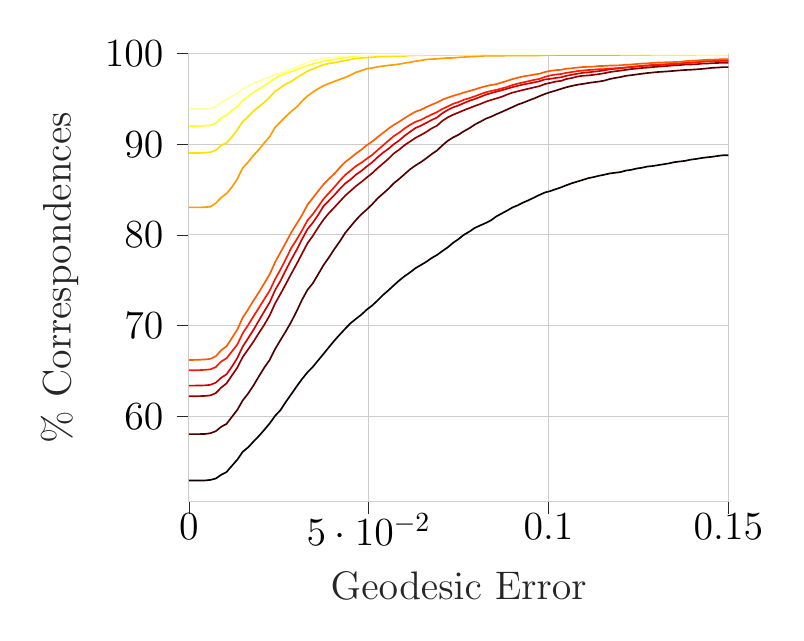
\begin{tikzpicture}

\definecolor{black1000}{RGB}{10,0,0}
\definecolor{darkred14400}{RGB}{144,0,0}
\definecolor{darkslategray38}{RGB}{38,38,38}
\definecolor{gold2552250}{RGB}{255,225,0}
\definecolor{lightgray204}{RGB}{204,204,204}
\definecolor{maroon7600}{RGB}{76,0,0}
\definecolor{orange2551570}{RGB}{255,157,0}
\definecolor{orangered255910}{RGB}{255,91,0}
\definecolor{palegoldenrod255255156}{RGB}{255,255,156}
\definecolor{red21000}{RGB}{210,0,0}
\definecolor{red255230}{RGB}{255,23,0}
\definecolor{yellow25525554}{RGB}{255,255,54}



\Large
\begin{axis}[
axis line style={lightgray204},
legend style={
  fill opacity=0.8,
  draw opacity=1,
  text opacity=1,
  at={(0.03,0.97)},
  anchor=north west,
  draw=lightgray204
},
tick align=outside,
tick pos=left,
x grid style={lightgray204},
xtick = {0,0.05,0.1,0.15},
xticklabel style={yshift= 5pt},
xlabel=\textcolor{darkslategray38}{Geodesic Error},
xmajorgrids,
xmin=0, xmax=0.15,
xtick style={color=darkslategray38},
y grid style={lightgray204},
ylabel=\textcolor{darkslategray38}{\% Correspondences},
ymajorgrids,
ymin=50.5604249667995, ymax=100,
ytick style={color=darkslategray38}
]
\addplot [semithick, black1000, forget plot]
table {%
0 52.912793271359
0.0015 52.912793271359
0.003 52.912793271359
0.0045 52.9194333776007
0.006 52.9769809650288
0.0075 53.1297034085879
0.009 53.5347498893316
0.0105 53.8468348826915
0.012 54.5396193005755
0.0135 55.2146967684816
0.015 56.0823373173971
0.0165 56.5692784417884
0.018 57.2111553784861
0.0195 57.8242585214697
0.021 58.5059760956175
0.0225 59.2120407259849
0.024 60.0442673749446
0.0255 60.6817175741478
0.027 61.5958388667552
0.0285 62.4324922532094
0.03 63.2979194333776
0.0315 64.1102257636122
0.033 64.8450641876937
0.0345 65.4493138556884
0.036 66.1775121735281
0.0375 66.896857016379
0.039 67.6339088092076
0.0405 68.3532536520584
0.042 69.0172642762284
0.0435 69.6591412129261
0.045 70.2678176184152
0.0465 70.7481186365649
0.048 71.2129260734838
0.0495 71.7662682602921
0.051 72.2155821159805
0.0525 72.7822045152722
0.054 73.3709606020363
0.0555 73.8866755201416
0.057 74.4378043382028
0.0585 74.9690128375387
0.06 75.4471004869411
0.0615 75.8565737051793
0.063 76.3235945108455
0.0645 76.6710934041612
0.066 77.0252324037185
0.0675 77.4435590969456
0.069 77.7844178840195
0.0705 78.2204515272244
0.072 78.6299247454626
0.0735 79.1323594510846
0.075 79.5440460380699
0.0765 80.0154935812306
0.078 80.360779105799
0.0795 80.7658255865427
0.081 81.0424966799469
0.0825 81.3014608233732
0.084 81.6046923417442
0.0855 82.0385126162019
0.087 82.3616644532979
0.0885 82.6826029216468
0.09 83.0256750774679
0.0915 83.2713590084108
0.093 83.576803895529
0.0945 83.8291279327136
0.096 84.1212926073484
0.0975 84.4090305444887
0.099 84.6746347941567
0.1005 84.8295706064631
0.102 85.0420540061974
0.1035 85.2434705621957
0.105 85.4803010181496
0.1065 85.6972111553785
0.108 85.8764940239044
0.1095 86.0579902611775
0.111 86.2483399734396
0.1125 86.3700752545374
0.114 86.518370960602
0.1155 86.6356795042054
0.117 86.7706949977867
0.1185 86.8503762726871
0.12 86.9234174413458
0.1215 87.0916334661355
0.123 87.1757414785303
0.1245 87.315183709606
0.126 87.4059318282426
0.1275 87.5387339530766
0.129 87.5940681717574
0.1305 87.6958831341301
0.132 87.7866312527667
0.1335 87.8884462151394
0.135 88.0212483399734
0.1365 88.0942895086321
0.138 88.1651173085436
0.1395 88.2957060646304
0.141 88.3709606020363
0.1425 88.4749889331563
0.144 88.5502434705622
0.1455 88.6122177954847
0.147 88.7051792828685
0.1485 88.7782204515272
0.15 88.7782204515272
};
\addplot [semithick, maroon7600, forget plot]
table {%
0 58.0301018149624
0.0015 58.0301018149624
0.003 58.0301018149624
0.0045 58.0433820274458
0.006 58.1230633023462
0.0075 58.3466135458167
0.009 58.833554670208
0.0105 59.1522797698096
0.012 59.933598937583
0.0135 60.7104913678619
0.015 61.7485613103143
0.0165 62.5055334218681
0.018 63.406374501992
0.0195 64.402390438247
0.021 65.369632580788
0.0225 66.2151394422311
0.024 67.4103585657371
0.0255 68.4108012394865
0.027 69.3846834882692
0.0285 70.4249667994688
0.03 71.5914121292607
0.0315 72.8574590526781
0.033 73.9353696325808
0.0345 74.6702080566622
0.036 75.6772908366534
0.0375 76.6954404603807
0.039 77.5365205843294
0.0405 78.4484285081895
0.042 79.2917220008854
0.0435 80.2257636122178
0.045 80.9451084550686
0.0465 81.6533864541833
0.048 82.2797698096503
0.0495 82.8065515714918
0.051 83.3820274457725
0.0525 84.0283311199646
0.054 84.5551128818061
0.0555 85.0841080123949
0.057 85.692784417884
0.0585 86.1775121735281
0.06 86.6998671978751
0.0615 87.2266489597167
0.063 87.6516157591855
0.0645 88.0146082337318
0.066 88.4395750332006
0.0675 88.9043824701195
0.069 89.3050022133688
0.0705 89.8738379814077
0.072 90.3740593182824
0.0735 90.7547587428066
0.075 91.0491367861886
0.0765 91.4364763169544
0.078 91.7662682602921
0.0795 92.1646746347941
0.081 92.4701195219123
0.0825 92.7999114652501
0.084 93.0256750774679
0.0855 93.3023461708721
0.087 93.5590969455511
0.0885 93.8269145639663
0.09 94.0969455511288
0.0915 94.373616644533
0.093 94.5794599380257
0.0945 94.8207171314742
0.096 95.0442673749447
0.0975 95.3010181496238
0.099 95.5444887118194
0.1005 95.7436918990704
0.102 95.9119079238601
0.1035 96.1044710048694
0.105 96.2859672421426
0.1065 96.4298362107127
0.108 96.555998229305
0.1095 96.6445329791943
0.111 96.746347941567
0.1125 96.8282425852147
0.114 96.9101372288623
0.1155 97.0097388224878
0.117 97.1845949535192
0.1185 97.3041168658699
0.12 97.4037184594953
0.1215 97.5409473218238
0.123 97.6117751217353
0.1245 97.6914563966356
0.126 97.7755644090305
0.1275 97.846392208942
0.129 97.9061531651172
0.1305 97.9637007525453
0.132 97.999114652501
0.1335 98.0411686586985
0.135 98.0898627711376
0.1365 98.140770252324
0.138 98.1850376272686
0.1395 98.2093846834882
0.141 98.2492253209384
0.1425 98.2957060646303
0.144 98.3532536520584
0.1455 98.4218680832226
0.147 98.4506418769367
0.1485 98.4949092518813
0.15 98.4949092518813
};
\addplot [semithick, darkred14400, forget plot]
table {%
0 62.2045152722444
0.0015 62.2045152722444
0.003 62.2177954847278
0.0045 62.2377158034529
0.006 62.2974767596282
0.0075 62.5453740593183
0.009 63.1540504648074
0.0105 63.6254980079681
0.012 64.5019920318725
0.0135 65.3674192120407
0.015 66.5382912793271
0.0165 67.3727312970341
0.018 68.2337317397078
0.0195 69.1854803010182
0.021 70.0929614873838
0.0225 71.1266046923418
0.024 72.4391323594512
0.0255 73.4949092518814
0.027 74.5949535192563
0.0285 75.7171314741036
0.03 76.8016821602479
0.0315 77.9393536963258
0.033 79.0792386011509
0.0345 79.89597166888
0.036 80.8455068614431
0.0375 81.7042939353696
0.039 82.419212040726
0.0405 83.045595396193
0.042 83.6874723328906
0.0435 84.3315626383355
0.045 84.8605577689243
0.0465 85.3895528995131
0.048 85.8410801239487
0.0495 86.3368747233289
0.051 86.8083222664896
0.0525 87.3683045595396
0.054 87.8707392651616
0.0555 88.3886675520142
0.057 88.9774236387782
0.0585 89.402390438247
0.06 89.8959716688801
0.0615 90.2899513058876
0.063 90.6972111553785
0.0645 91.0048694112439
0.066 91.3501549358123
0.0675 91.7419212040726
0.069 92.0429393536963
0.0705 92.5785745905268
0.072 92.9570606463036
0.0735 93.2536520584329
0.075 93.4971226206285
0.0765 93.7516600265604
0.078 93.9774236387782
0.0795 94.2164674634794
0.081 94.4245241257193
0.0825 94.6746347941567
0.084 94.8694112439132
0.0855 95.0464807436919
0.087 95.227976980965
0.0885 95.4780876494024
0.09 95.6905710491368
0.0915 95.8366533864542
0.093 95.9849490925189
0.0945 96.128818061089
0.096 96.2682602921647
0.0975 96.4032757857459
0.099 96.6334661354581
0.1005 96.7640548915449
0.102 96.9101372288623
0.1035 96.9853917662682
0.105 97.1890216910137
0.1065 97.3019034971226
0.108 97.4546259406817
0.1095 97.5453740593182
0.111 97.580787959274
0.1125 97.6516157591854
0.114 97.7268702965914
0.1155 97.8264718902169
0.117 97.9526339088092
0.1185 98.0389552899512
0.12 98.1119964586099
0.1215 98.1961044710048
0.123 98.2846392208941
0.1245 98.3333333333333
0.126 98.4041611332447
0.1275 98.4440017706949
0.129 98.5081894643647
0.1305 98.5502434705621
0.132 98.5922974767595
0.1335 98.6454183266931
0.135 98.6963258078795
0.1365 98.7250996015936
0.138 98.7782204515272
0.1395 98.7915006640106
0.141 98.8092076139884
0.1425 98.8778220451526
0.144 98.8933156263832
0.1455 98.9353696325807
0.147 98.9552899513058
0.1485 98.9862771137671
0.15 98.9862771137671
};
\addplot [semithick, red21000, forget plot]
table {%
0 63.377600708278
0.0015 63.377600708278
0.003 63.3908809207614
0.0045 63.4019477644976
0.006 63.4617087206728
0.0075 63.6985391766268
0.009 64.240814519699
0.0105 64.6281540504648
0.012 65.4692341744135
0.0135 66.4254094732183
0.015 67.6826029216468
0.0165 68.5989375830013
0.018 69.535192563081
0.0195 70.5555555555555
0.021 71.5626383355467
0.0225 72.5630810092961
0.024 73.908809207614
0.0255 74.9291722000885
0.027 76.1420982735724
0.0285 77.2797698096503
0.03 78.3576803895529
0.0315 79.5285524568393
0.033 80.626383355467
0.0345 81.3523683045595
0.036 82.220008853475
0.0375 83.1961044710048
0.039 83.7915006640106
0.0405 84.3957503320053
0.042 85.0774679061532
0.0435 85.6772908366534
0.045 86.1133244798584
0.0465 86.651173085436
0.048 87.0628596724214
0.0495 87.5542275343072
0.051 88.0057547587428
0.0525 88.5635236830456
0.054 89.0659583886675
0.0555 89.4931385568836
0.057 89.9977866312528
0.0585 90.4138999557326
0.06 90.9274015050908
0.0615 91.3634351482957
0.063 91.7795484727755
0.0645 92.0385126162019
0.066 92.3505976095617
0.0675 92.6604692341744
0.069 92.9437804338203
0.0705 93.4196547144754
0.072 93.7737937140327
0.0735 94.0637450199203
0.075 94.2740150509075
0.0765 94.5374059318282
0.078 94.7830898627711
0.0795 94.9800796812749
0.081 95.2102700309872
0.0825 95.4515272244357
0.084 95.6285967242143
0.0855 95.7901726427623
0.087 95.9561752988047
0.0885 96.1155378486056
0.09 96.2970340858787
0.0915 96.4453297919433
0.093 96.5869853917663
0.0945 96.6976538291279
0.096 96.8149623727313
0.0975 96.9433377600707
0.099 97.1403275785746
0.1005 97.2045152722443
0.102 97.3063302346171
0.1035 97.381584772023
0.105 97.5475874280655
0.1065 97.6560424966799
0.108 97.7689243027888
0.1095 97.8685258964143
0.111 97.9172200088534
0.1125 97.9902611775121
0.114 98.0566622399291
0.1155 98.140770252324
0.117 98.2558654271801
0.1185 98.3178397521027
0.12 98.3731739707835
0.1215 98.4484285081894
0.123 98.5126162018592
0.1245 98.5568835768039
0.126 98.6277113767153
0.1275 98.6542718016821
0.129 98.7051792828685
0.1305 98.7317397078353
0.132 98.7583001328021
0.1335 98.8114209827357
0.135 98.8424081451969
0.1365 98.8933156263833
0.138 98.9707835325364
0.1395 98.9884904825143
0.141 99.0150509074811
0.1425 99.1102257636121
0.144 99.1389995573262
0.1455 99.1611332447985
0.147 99.1788401947763
0.1485 99.1965471447542
0.15 99.1965471447542
};
\addplot [semithick, red255230, forget plot]
table {%
0 65.0730411686587
0.0015 65.0730411686587
0.003 65.0863213811421
0.0045 65.1173085436034
0.006 65.1726427622842
0.0075 65.4205400619743
0.009 66.0314298362107
0.0105 66.3877822045152
0.012 67.1469676848163
0.0135 67.912793271359
0.015 69.1478530323152
0.0165 70.0531208499336
0.018 71.0159362549801
0.0195 71.9632580787959
0.021 72.9172200088535
0.0225 73.8512616201859
0.024 75.1128818061089
0.0255 76.1752988047809
0.027 77.3505976095617
0.0285 78.5590969455511
0.03 79.4864984506419
0.0315 80.5090748118637
0.033 81.5914121292608
0.0345 82.2952633908809
0.036 83.1274900398406
0.0375 83.9796370075255
0.039 84.630367419212
0.0405 85.2788844621514
0.042 85.9849490925188
0.0435 86.6157591854803
0.045 87.0982735723771
0.0465 87.5918548030102
0.048 87.9659141212926
0.0495 88.406374501992
0.051 88.8180610889774
0.0525 89.3492695883134
0.054 89.8716246126605
0.0555 90.3917662682603
0.057 90.8964143426295
0.0585 91.2749003984064
0.06 91.7330677290837
0.0615 92.1292607348384
0.063 92.4634794156706
0.0645 92.675962815405
0.066 92.9791943337759
0.0675 93.2691456396635
0.069 93.5413899955732
0.0705 93.8888888888889
0.072 94.1677733510402
0.0735 94.4599380256751
0.075 94.6458610004427
0.0765 94.9003984063745
0.078 95.0774679061532
0.0795 95.2766710934042
0.081 95.5090748118637
0.0825 95.7171314741036
0.084 95.8654271801682
0.0855 95.9871624612661
0.087 96.1487383798141
0.0885 96.3103142983621
0.09 96.5250110668437
0.0915 96.6843736166445
0.093 96.8193891102258
0.0945 96.954404603807
0.096 97.0916334661355
0.0975 97.1978751660026
0.099 97.4236387782205
0.1005 97.5830013280212
0.102 97.6826029216467
0.1035 97.742363877822
0.105 97.8685258964143
0.1065 97.9614873837981
0.108 98.0588756086764
0.1095 98.1208499335989
0.111 98.1761841522797
0.1125 98.2138114209827
0.114 98.2691456396635
0.1155 98.2824258521469
0.117 98.3377600708278
0.1185 98.3709606020363
0.12 98.4152279769809
0.1215 98.4594953519256
0.123 98.5126162018592
0.1245 98.5834440017707
0.126 98.6609119079238
0.1275 98.6808322266489
0.129 98.7494466578131
0.1305 98.7782204515272
0.132 98.8025675077467
0.1335 98.833554670208
0.135 98.862328463922
0.1365 98.891102257636
0.138 98.966356795042
0.1395 98.9884904825143
0.141 99.0349712262062
0.1425 99.0947321823815
0.144 99.1412129260734
0.1455 99.1677733510402
0.147 99.1832669322708
0.1485 99.2142540947321
0.15 99.2142540947321
};
\addplot [semithick, orangered255910, forget plot]
table {%
0 66.2062859672422
0.0015 66.2107127047366
0.003 66.2284196547145
0.0045 66.2638335546702
0.006 66.3258078795928
0.0075 66.6113324479859
0.009 67.2664895971669
0.0105 67.713590084108
0.012 68.6232846392209
0.0135 69.5573262505534
0.015 70.8787073926516
0.0165 71.7751217352811
0.018 72.7600708277999
0.0195 73.6675520141656
0.021 74.6591412129261
0.0225 75.6595838866755
0.024 76.983178397521
0.0255 78.0743691899071
0.027 79.1589198760514
0.0285 80.2700309871625
0.03 81.2372731297034
0.0315 82.1890216910137
0.033 83.3178397521027
0.0345 84.0748118636564
0.036 84.838424081452
0.0375 85.5843293492696
0.039 86.1930057547588
0.0405 86.7463479415671
0.042 87.4324922532094
0.0435 88.036741921204
0.045 88.4860557768924
0.0465 88.9774236387782
0.048 89.3957503320053
0.0495 89.89597166888
0.051 90.294378043382
0.0525 90.7857459052678
0.054 91.2439132359451
0.0555 91.7131474103586
0.057 92.1336874723329
0.0585 92.4789729969013
0.06 92.8773793714033
0.0615 93.2425852146968
0.063 93.5790172642762
0.0645 93.7870739265162
0.066 94.0836653386454
0.0675 94.3559096945551
0.069 94.5927401505091
0.0705 94.9026117751217
0.072 95.132802124834
0.0735 95.3342186808322
0.075 95.5046480743692
0.0765 95.7038512616202
0.078 95.8610004426738
0.0795 96.0336432049579
0.081 96.2262062859673
0.0825 96.3922089420097
0.084 96.5227976980965
0.0855 96.6157591854803
0.087 96.8061088977424
0.0885 96.983178397521
0.09 97.1779548472776
0.0915 97.3373173970783
0.093 97.4811863656485
0.0945 97.5675077467906
0.096 97.6803895528995
0.0975 97.7733510402833
0.099 97.9592740150509
0.1005 98.083222664896
0.102 98.1673306772908
0.1035 98.2027445772465
0.105 98.3266932270916
0.1065 98.3731739707835
0.108 98.4506418769366
0.1095 98.5104028331119
0.111 98.5258964143425
0.1125 98.5568835768038
0.114 98.6166445329791
0.1155 98.634351482957
0.117 98.6697653829127
0.1185 98.6808322266489
0.12 98.7029659141212
0.1215 98.758300132802
0.123 98.7892872952633
0.1245 98.8446215139441
0.126 98.8933156263833
0.1275 98.9176626826029
0.129 98.9685701637892
0.1305 99.0061974324922
0.132 99.0239043824701
0.1335 99.0416113324479
0.135 99.0593182824258
0.1365 99.0814519698981
0.138 99.156706507304
0.1395 99.1899070385126
0.141 99.2253209384683
0.1425 99.2673749446657
0.144 99.3072155821159
0.1455 99.3204957945993
0.147 99.3492695883133
0.1485 99.3846834882691
0.15 99.3846834882691
};
\addplot [semithick, orange2551570, forget plot]
table {%
0 83.0278884462151
0.0015 83.0278884462151
0.003 83.0278884462151
0.0045 83.0522355024347
0.006 83.1053563523683
0.0075 83.4838424081452
0.009 84.1057990261178
0.0105 84.5595396193006
0.012 85.2810978308986
0.0135 86.1708720672864
0.015 87.3837981407702
0.0165 88.0190349712262
0.018 88.7605135015493
0.0195 89.3979637007525
0.021 90.1438689685702
0.0225 90.834440017707
0.024 91.8525896414343
0.0255 92.4656927844179
0.027 93.0610889774237
0.0285 93.6122177954847
0.03 94.1013722886233
0.0315 94.7476759628154
0.033 95.3142983621071
0.0345 95.7392651615759
0.036 96.1199645861001
0.0375 96.4586100044267
0.039 96.6976538291279
0.0405 96.9212040725985
0.042 97.1513944223108
0.0435 97.3594510845507
0.045 97.6250553342187
0.0465 97.9349269588313
0.048 98.1097830898627
0.0495 98.3266932270916
0.051 98.3975210270031
0.0525 98.5325365205842
0.054 98.6122177954846
0.0555 98.6941124391323
0.057 98.7538733953076
0.0585 98.824701195219
0.06 98.9530765825586
0.0615 99.0349712262062
0.063 99.1522797698096
0.0645 99.2319610447099
0.066 99.3426294820716
0.0675 99.3780433820273
0.069 99.4090305444886
0.0705 99.4665781319167
0.072 99.5086321381141
0.0735 99.5152722443558
0.075 99.5683930942894
0.0765 99.6060203629924
0.078 99.6480743691898
0.0795 99.6746347941566
0.081 99.7122620628595
0.0825 99.7432492253208
0.084 99.754316069057
0.0855 99.7587428065515
0.087 99.7609561752987
0.0885 99.7631695440459
0.09 99.7653829127932
0.0915 99.7698096502876
0.093 99.7742363877821
0.0945 99.7742363877821
0.096 99.783089862771
0.0975 99.7897299690127
0.099 99.8162903939796
0.1005 99.820717131474
0.102 99.8251438689685
0.1035 99.8251438689685
0.105 99.8251438689685
0.1065 99.8251438689685
0.108 99.8251438689685
0.1095 99.8251438689685
0.111 99.8317839752102
0.1125 99.8317839752102
0.114 99.8384240814519
0.1155 99.8384240814519
0.117 99.8406374501992
0.1185 99.8428508189464
0.12 99.8450641876937
0.1215 99.8450641876937
0.123 99.8494909251881
0.1245 99.8494909251881
0.126 99.8517042939353
0.1275 99.8539176626826
0.129 99.8826914563966
0.1305 99.8826914563966
0.132 99.8826914563966
0.1335 99.8826914563966
0.135 99.8826914563966
0.1365 99.8826914563966
0.138 99.8849048251439
0.1395 99.8849048251439
0.141 99.9026117751217
0.1425 99.9026117751217
0.144 99.9026117751217
0.1455 99.9048251438689
0.147 99.9070385126162
0.1485 99.9070385126162
0.15 99.9070385126162
};
\addplot [semithick, gold2552250, forget plot]
table {%
0 89.0261177512173
0.0015 89.0283311199646
0.003 89.0283311199646
0.0045 89.0571049136786
0.006 89.1190792386012
0.0075 89.3182824258522
0.009 89.8649845064188
0.0105 90.1350154935812
0.012 90.8056662239929
0.0135 91.6002656042497
0.015 92.485613103143
0.0165 93.0212483399735
0.018 93.6586985391766
0.0195 94.1279327135901
0.021 94.6193005754759
0.0225 95.1837096060203
0.024 95.8410801239486
0.0255 96.2262062859672
0.027 96.6378928729526
0.0285 96.9189907038512
0.03 97.3262505533422
0.0315 97.6936697653829
0.033 98.0544488711819
0.0345 98.3089862771137
0.036 98.5436033643205
0.0375 98.7649402390438
0.039 98.9110225763612
0.0405 98.9818503762726
0.042 99.1124391323594
0.0435 99.2186808322266
0.045 99.3448428508189
0.0465 99.4577246569278
0.048 99.5064187693669
0.0495 99.5506861443116
0.051 99.5861000442673
0.0525 99.6414342629481
0.054 99.6569278441788
0.0555 99.6746347941566
0.057 99.6812749003983
0.0585 99.68791500664
0.06 99.7277556440902
0.0615 99.7786631252766
0.063 99.7941567065073
0.0645 99.7985834440017
0.066 99.8273572377157
0.0675 99.8339973439574
0.069 99.8362107127047
0.0705 99.8384240814519
0.072 99.8406374501992
0.0735 99.8406374501992
0.075 99.8561310314298
0.0765 99.8605577689242
0.078 99.8605577689242
0.0795 99.8627711376715
0.081 99.89597166888
0.0825 99.89597166888
0.084 99.89597166888
0.0855 99.89597166888
0.087 99.89597166888
0.0885 99.89597166888
0.09 99.89597166888
0.0915 99.89597166888
0.093 99.89597166888
0.0945 99.89597166888
0.096 99.89597166888
0.0975 99.89597166888
0.099 99.8981850376272
0.1005 99.8981850376272
0.102 99.9003984063744
0.1035 99.9003984063744
0.105 99.9003984063744
0.1065 99.9003984063744
0.108 99.9003984063744
0.1095 99.9003984063744
0.111 99.9003984063744
0.1125 99.9003984063744
0.114 99.9003984063744
0.1155 99.9003984063744
0.117 99.9003984063744
0.1185 99.9003984063744
0.12 99.9026117751217
0.1215 99.9026117751217
0.123 99.9026117751217
0.1245 99.9026117751217
0.126 99.9026117751217
0.1275 99.9026117751217
0.129 99.9203187250995
0.1305 99.9203187250995
0.132 99.9203187250995
0.1335 99.9203187250995
0.135 99.9203187250995
0.1365 99.9203187250995
0.138 99.9203187250995
0.1395 99.9203187250995
0.141 99.9203187250995
0.1425 99.9203187250995
0.144 99.9203187250995
0.1455 99.9203187250995
0.147 99.9203187250995
0.1485 99.9203187250995
0.15 99.9203187250995
};
\addplot [semithick, yellow25525554, forget plot]
table {%
0 91.9964586100044
0.0015 91.9986719787517
0.003 91.9986719787517
0.0045 92.0274457724657
0.006 92.0805666223993
0.0075 92.3085436033643
0.009 92.8818061088977
0.0105 93.1983178397521
0.012 93.7184594953519
0.0135 94.1434262948207
0.015 94.829570606463
0.0165 95.2368304559539
0.018 95.7193448428508
0.0195 96.0779105799026
0.021 96.4497565294378
0.0225 96.8459495351925
0.024 97.2664895971669
0.0255 97.5719344842851
0.027 97.817618415228
0.0285 97.9836210712705
0.03 98.2248782647189
0.0315 98.4528552456839
0.033 98.6564851704293
0.0345 98.8490482514387
0.036 98.9907038512616
0.0375 99.1611332447985
0.039 99.2629482071712
0.0405 99.3315626383355
0.042 99.4555112881806
0.0435 99.5462594068171
0.045 99.6347941567064
0.0465 99.734395750332
0.048 99.7742363877821
0.0495 99.8007968127489
0.051 99.8162903939796
0.0525 99.8317839752102
0.054 99.8339973439574
0.0555 99.8362107127046
0.057 99.8384240814519
0.0585 99.8428508189463
0.06 99.8539176626825
0.0615 99.8738379814076
0.063 99.8738379814076
0.0645 99.8738379814076
0.066 99.8937583001327
0.0675 99.8937583001327
0.069 99.8937583001327
0.0705 99.8937583001327
0.072 99.89597166888
0.0735 99.89597166888
0.075 99.9136786188578
0.0765 99.9136786188578
0.078 99.9136786188578
0.0795 99.9136786188578
0.081 99.9158919876051
0.0825 99.9181053563523
0.084 99.9181053563523
0.0855 99.9181053563523
0.087 99.9203187250995
0.0885 99.9203187250995
0.09 99.9203187250995
0.0915 99.9203187250995
0.093 99.9203187250995
0.0945 99.9203187250995
0.096 99.9203187250995
0.0975 99.9203187250995
0.099 99.9203187250995
0.1005 99.9203187250995
0.102 99.9203187250995
0.1035 99.9203187250995
0.105 99.9203187250995
0.1065 99.9203187250995
0.108 99.9203187250995
0.1095 99.9203187250995
0.111 99.9203187250995
0.1125 99.9203187250995
0.114 99.9203187250995
0.1155 99.9203187250995
0.117 99.9203187250995
0.1185 99.9203187250995
0.12 99.9203187250995
0.1215 99.9203187250995
0.123 99.9203187250995
0.1245 99.9203187250995
0.126 99.9203187250995
0.1275 99.9203187250995
0.129 99.9203187250995
0.1305 99.9203187250995
0.132 99.9203187250995
0.1335 99.9203187250995
0.135 99.9203187250995
0.1365 99.9203187250995
0.138 99.9203187250995
0.1395 99.9203187250995
0.141 99.9203187250995
0.1425 99.9203187250995
0.144 99.9203187250995
0.1455 99.9203187250995
0.147 99.9203187250995
0.1485 99.9203187250995
0.15 99.9203187250995
};
\addplot [semithick, palegoldenrod255255156, forget plot]
table {%
0 93.8733953076583
0.0015 93.8756086764055
0.003 93.8756086764055
0.0045 93.8866755201417
0.006 93.9353696325809
0.0075 94.1235059760957
0.009 94.6193005754758
0.0105 94.9092518813635
0.012 95.2899513058876
0.0135 95.5621956617973
0.015 96.1066843736166
0.0165 96.394422310757
0.018 96.7330677290836
0.0195 96.9433377600708
0.021 97.211155378486
0.0225 97.3948649845064
0.024 97.6914563966357
0.0255 97.788844621514
0.027 98.0699424524126
0.0285 98.2492253209384
0.03 98.501549358123
0.0315 98.7782204515272
0.033 99.0548915449314
0.0345 99.2363877822045
0.036 99.355909694555
0.0375 99.4710048694112
0.039 99.5219123505975
0.0405 99.6015936254979
0.042 99.7011952191234
0.0435 99.7587428065515
0.045 99.7875166002655
0.0465 99.7985834440017
0.048 99.8273572377158
0.0495 99.8384240814519
0.051 99.8539176626826
0.0525 99.8671978751659
0.054 99.8782647189021
0.0555 99.8871181938911
0.057 99.9092518813634
0.0585 99.9092518813634
0.06 99.9114652501107
0.0615 99.9136786188579
0.063 99.9136786188579
0.0645 99.9136786188579
0.066 99.933598937583
0.0675 99.933598937583
0.069 99.933598937583
0.0705 99.933598937583
0.072 99.9358123063302
0.0735 99.9358123063302
0.075 99.9535192563081
0.0765 99.9535192563081
0.078 99.9535192563081
0.0795 99.9535192563081
0.081 99.9557326250553
0.0825 99.9579459938026
0.084 99.9579459938026
0.0855 99.9579459938026
0.087 99.9601593625498
0.0885 99.9601593625498
0.09 99.9601593625498
0.0915 99.9601593625498
0.093 99.9601593625498
0.0945 99.9601593625498
0.096 99.9601593625498
0.0975 99.9601593625498
0.099 99.9601593625498
0.1005 99.9601593625498
0.102 99.9601593625498
0.1035 99.9601593625498
0.105 99.9601593625498
0.1065 99.9601593625498
0.108 99.9601593625498
0.1095 99.9601593625498
0.111 99.9601593625498
0.1125 99.9601593625498
0.114 99.9601593625498
0.1155 99.9601593625498
0.117 99.9601593625498
0.1185 99.9601593625498
0.12 99.9601593625498
0.1215 99.9601593625498
0.123 99.9601593625498
0.1245 99.9601593625498
0.126 99.9601593625498
0.1275 99.9601593625498
0.129 99.9601593625498
0.1305 99.9601593625498
0.132 99.9601593625498
0.1335 99.9601593625498
0.135 99.9601593625498
0.1365 99.9601593625498
0.138 99.9601593625498
0.1395 99.9601593625498
0.141 99.9601593625498
0.1425 99.9601593625498
0.144 99.9601593625498
0.1455 99.9601593625498
0.147 99.9601593625498
0.1485 99.9601593625498
0.15 99.9601593625498
};
\addplot [semithick, white, forget plot]
table {%
0 94.1921204072599
0.0015 94.1943337760071
0.003 94.1943337760071
0.0045 94.2054006197433
0.006 94.2540947321824
0.0075 94.4422310756972
0.009 94.9468791500665
0.0105 95.2567507746791
0.012 95.6662239929172
0.0135 95.9096945551128
0.015 96.385568835768
0.0165 96.6954404603807
0.018 96.99203187251
0.0195 97.1691013722886
0.021 97.4656927844178
0.0225 97.6980965028773
0.024 98.0256750774679
0.0255 98.1363435148295
0.027 98.4639220894201
0.0285 98.5967242142541
0.03 98.8092076139885
0.0315 99.0106241699867
0.033 99.1810535635236
0.0345 99.4046038069942
0.036 99.5285524568393
0.0375 99.6458610004426
0.039 99.696768481629
0.0405 99.7388224878264
0.042 99.8229305002213
0.0435 99.8317839752102
0.045 99.8517042939353
0.0465 99.858344400177
0.048 99.8826914563966
0.0495 99.8871181938911
0.051 99.8937583001328
0.0525 99.9048251438689
0.054 99.9070385126162
0.0555 99.9092518813634
0.057 99.9092518813634
0.0585 99.9092518813634
0.06 99.9114652501107
0.0615 99.9136786188579
0.063 99.9158919876051
0.0645 99.9158919876051
0.066 99.9380256750775
0.0675 99.9380256750775
0.069 99.9380256750775
0.0705 99.9380256750775
0.072 99.9402390438247
0.0735 99.9402390438247
0.075 99.9579459938025
0.0765 99.9579459938025
0.078 99.9579459938025
0.0795 99.9579459938025
0.081 99.9601593625498
0.0825 99.9601593625498
0.084 99.9601593625498
0.0855 99.9601593625498
0.087 99.9601593625498
0.0885 99.9601593625498
0.09 99.9601593625498
0.0915 99.9601593625498
0.093 99.9601593625498
0.0945 99.9601593625498
0.096 99.9601593625498
0.0975 99.9601593625498
0.099 99.9601593625498
0.1005 99.9601593625498
0.102 99.9601593625498
0.1035 99.9601593625498
0.105 99.9601593625498
0.1065 99.9601593625498
0.108 99.9601593625498
0.1095 99.9601593625498
0.111 99.9601593625498
0.1125 99.9601593625498
0.114 99.9601593625498
0.1155 99.9601593625498
0.117 99.9601593625498
0.1185 99.9601593625498
0.12 99.9601593625498
0.1215 99.9601593625498
0.123 99.9601593625498
0.1245 99.9601593625498
0.126 99.9601593625498
0.1275 99.9601593625498
0.129 99.9601593625498
0.1305 99.9601593625498
0.132 99.9601593625498
0.1335 99.9601593625498
0.135 99.9601593625498
0.1365 99.9601593625498
0.138 99.9601593625498
0.1395 99.9601593625498
0.141 99.9601593625498
0.1425 99.9601593625498
0.144 99.9601593625498
0.1455 99.9601593625498
0.147 99.9601593625498
0.1485 99.9601593625498
0.15 99.9601593625498
};
\end{axis}

\end{tikzpicture}
}
    \resizebox{0.49\linewidth}{!}{
    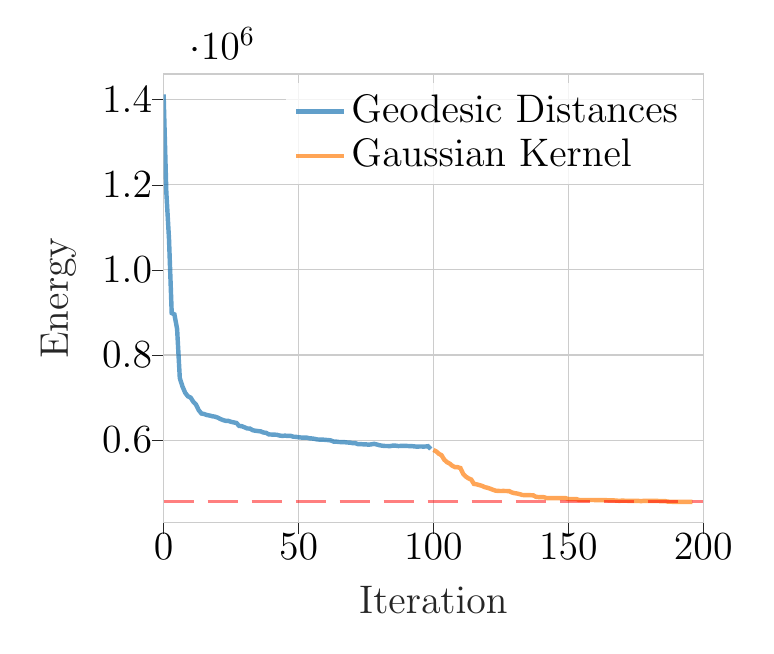
\begin{tikzpicture}

\definecolor{darkorange25512714}{RGB}{255,127,14}
\definecolor{darkslategray38}{RGB}{38,38,38}
\definecolor{lightgray204}{RGB}{204,204,204}
\definecolor{steelblue31119180}{RGB}{31,119,180}

\Large
\begin{axis}[
axis line style={lightgray204},
legend cell align={left},
legend style={fill opacity=0.8, draw opacity=1, text opacity=1, draw=none},
tick align=outside,
tick pos=left,
x grid style={lightgray204},
xlabel=\textcolor{darkslategray38}{Iteration},
xmajorgrids,
xmin=0, xmax=200,
xtick style={color=darkslategray38},
y grid style={lightgray204},
ylabel=\textcolor{darkslategray38}{Energy},
ymajorgrids,
xticklabel style={yshift= 5pt},
yticklabel style={xshift= 5pt},
ymin=406793.434551037, ymax=1460495.06139121,
ytick style={color=darkslategray38},
ytick={400000,600000,800000,1000000,1200000,1400000,1600000},
yticklabels={0.4,0.6,0.8,1.0,1.2,1.4,1.6}
]
\addplot [ultra thick, steelblue31119180, opacity=0.7]
table {%
0 1412599.53289847
1 1183293.77062305
2 1072454.6975754
3 898482.753120199
4 895513.465773958
5 861165.121138548
6 745710.510909138
7 725822.194337174
8 711194.094283449
9 702845.217672286
10 699956.366642935
11 690091.676691849
12 683512.468663089
13 670394.810387172
14 662531.853289157
15 661283.563884537
16 658912.712604156
17 657761.436602939
18 656099.394278964
19 655082.938715587
20 653025.401642406
21 649695.31989293
22 647076.057273849
23 645285.878078882
24 645012.821138859
25 642893.777253901
26 641544.632198263
27 640242.039463242
28 633228.297661631
29 632648.501476486
30 629989.009194106
31 627303.857346239
32 627013.617889443
33 623208.217561243
34 621941.868290954
35 621202.415953106
36 620380.197402601
37 617807.079543611
38 616974.375787247
39 613343.771662781
40 613021.882862556
41 612794.081019129
42 612439.243610229
43 610628.68898855
44 609848.354258433
45 610443.81083058
46 609693.324223531
47 610074.206729221
48 608031.165399297
49 607629.705308602
50 606638.107575965
51 605984.900534482
52 605916.949109419
53 605813.03797345
54 604262.320120821
55 603764.1751954
56 602837.757346848
57 601391.782918322
58 601157.596220475
59 601123.542646458
60 600474.238052119
61 599996.925854989
62 599157.437784079
63 596513.444950086
64 596381.941649309
65 595510.394673576
66 595202.489398315
67 595165.722495269
68 594367.110504942
69 594055.9940645
70 592900.371104277
71 592885.2828775
72 590598.814343286
73 590661.779999414
74 590002.082943428
75 589938.29574777
76 589121.071902582
77 589957.143187013
78 591111.174671788
79 589686.549271123
80 587873.885021586
81 586808.061773484
82 586143.282542341
83 586030.072096886
84 585893.271688835
85 587086.748757131
86 586913.379231967
87 585955.48156708
88 586348.192112311
89 586333.303944257
90 586330.755202951
91 585882.080217232
92 585713.905784788
93 585141.496080228
94 584504.096818426
95 584993.277509551
96 584807.718793883
97 584845.291712538
98 585615.28282306
99 578886.853490675
};
\addlegendentry{Geodesic Distances}
\addplot [ultra thick, darkorange25512714, opacity=0.7]
table {%
100 576840.021402506
101 573530.952997623
102 567924.947849655
103 564379.118272291
104 554017.619681238
105 548102.527810449
106 544845.820683948
107 539614.350585595
108 536378.545716367
109 536261.087739481
110 534273.19758171
111 520882.404063444
112 514231.523811859
113 509932.280156059
114 507244.337288239
115 497030.195362117
116 496029.794819013
117 494256.945363337
118 492368.307323401
119 489450.59238252
120 487972.472939164
121 485781.882601781
122 483384.576253682
123 481120.692590119
124 480479.449344539
125 480347.378035902
126 480474.779354289
127 480272.831157448
128 480136.821383942
129 477092.45274907
130 475298.750603847
131 474461.412423961
132 472837.595204226
133 470872.134176471
134 470779.83527647
135 470557.038687321
136 470425.952850023
137 470114.277416967
138 466733.061625208
139 466038.781682035
140 465997.785615338
141 465702.627932939
142 463677.236469406
143 463677.236469406
144 463526.968502686
145 463613.353369596
146 463756.321559119
147 463398.60316162
148 463398.60316162
149 463538.801183693
150 461463.1988533
151 461284.919335796
152 461285.389410617
153 461298.629044072
154 459127.055741884
155 459218.819948569
156 459126.164127098
157 459126.164127098
158 459132.474202224
159 459132.474202224
160 459067.376111775
161 459058.244597648
162 459018.754495017
163 458908.856551856
164 458834.306698186
165 458251.07859838
166 458132.308423048
167 458132.308423048
168 457586.333582372
169 457149.95343917
170 457807.711916646
171 457388.451009342
172 457321.730705592
173 457321.730705592
174 457321.730705592
175 457321.730705592
176 457036.656321891
177 456517.127315651
178 457203.6052235
179 457203.6052235
180 456992.743887026
181 456992.743887026
182 456992.743887026
183 457003.555488247
184 456628.392774066
185 456371.173240389
186 456371.173240389
187 455206.561356197
188 455062.504217137
189 454871.926787803
190 454939.016781403
191 454979.948351088
192 454765.030021894
193 454688.963043772
194 454754.987391642
195 454761.298556856
196 454736.419213906
};
\addlegendentry{Gaussian Kernel}
\path [draw=red, draw opacity=0.5, very thick, dash pattern=on 11.1pt off 4.8pt]
(axis cs:0,455693.978434343)
--(axis cs:200,455693.978434343);

\end{axis}

\end{tikzpicture}
}
        \caption{FAUST}
    \end{subfigure}

        \begin{subfigure}[b]{\linewidth}
    \resizebox{0.49\linewidth}{!}{
    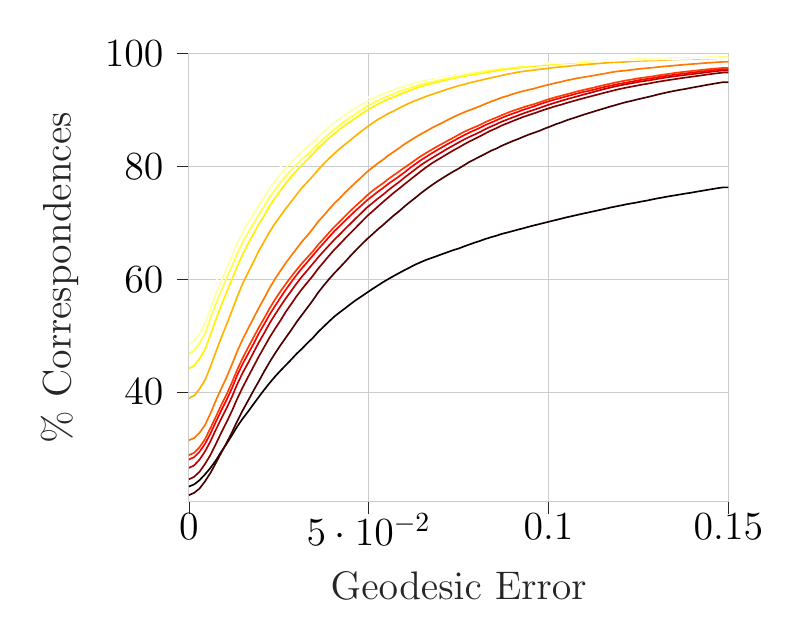
\begin{tikzpicture}

\definecolor{black1000}{RGB}{10,0,0}
\definecolor{darkorange2551200}{RGB}{255,120,0}
\definecolor{darkslategray38}{RGB}{38,38,38}
\definecolor{firebrick19100}{RGB}{191,0,0}
\definecolor{lightgray204}{RGB}{204,204,204}
\definecolor{maroon13100}{RGB}{131,0,0}
\definecolor{maroon7000}{RGB}{70,0,0}
\definecolor{orange2551800}{RGB}{255,180,0}
\definecolor{orangered255600}{RGB}{255,60,0}
\definecolor{palegoldenrod255255164}{RGB}{255,255,164}
\definecolor{red25400}{RGB}{254,0,0}
\definecolor{yellow2552430}{RGB}{255,243,0}
\definecolor{yellow25525573}{RGB}{255,255,73}

\Large
\begin{axis}[
axis line style={lightgray204},
tick align=outside,
tick pos=left,
x grid style={lightgray204},
xtick = {0,0.05,0.1,0.15},
xticklabel style={yshift= 5pt},
xlabel=\textcolor{darkslategray38}{Geodesic Error},
xmajorgrids,
xmin=0, xmax=0.15,
xtick style={color=darkslategray38},
y grid style={lightgray204},
ylabel=\textcolor{darkslategray38}{\% Correspondences},
ymajorgrids,
ymin=20.5604249667995, ymax=100,
ytick style={color=darkslategray38}
]
\addplot [semithick, black1000]
table {%
0 23.2664266426643
0.0015 23.6561656165617
0.003 24.4023402340234
0.0045 25.4194419441944
0.006 26.5616561656166
0.0075 27.8631863186319
0.009 29.4041404140414
0.0105 30.8406840684068
0.012 32.3645364536453
0.0135 33.9414941494149
0.015 35.3231323132313
0.0165 36.5679567956796
0.018 37.8838883888389
0.0195 39.1863186318632
0.021 40.4410441044105
0.0225 41.6417641764176
0.024 42.7713771377138
0.0255 43.8109810981098
0.027 44.7956795679568
0.0285 45.7848784878488
0.03 46.8199819981998
0.0315 47.7146714671467
0.033 48.7164716471647
0.0345 49.6165616561656
0.036 50.6948694869487
0.0375 51.6084608460846
0.039 52.5283528352835
0.0405 53.4149414941494
0.042 54.1629162916292
0.0435 54.8775877587759
0.045 55.6183618361836
0.0465 56.3348334833483
0.048 56.9585958595859
0.0495 57.6129612961296
0.051 58.2628262826283
0.0525 58.8730873087309
0.054 59.4869486948695
0.0555 60.0522052205221
0.057 60.5949594959496
0.0585 61.1134113411341
0.06 61.6309630963096
0.0615 62.1161116111611
0.063 62.6129612961296
0.0645 63.0315031503151
0.066 63.4338433843384
0.0675 63.7776777677768
0.069 64.1170117011701
0.0705 64.4770477047705
0.072 64.8145814581458
0.0735 65.1611161116112
0.075 65.4455445544554
0.0765 65.8145814581458
0.078 66.1611161116112
0.0795 66.4986498649865
0.081 66.8082808280828
0.0825 67.1521152115211
0.084 67.4545454545454
0.0855 67.7137713771377
0.087 68.041404140414
0.0885 68.2745274527453
0.09 68.5301530153015
0.0915 68.7983798379838
0.093 69.03600360036
0.0945 69.3051305130513
0.096 69.5508550855085
0.0975 69.7794779477947
0.099 70.026102610261
0.1005 70.2610261026103
0.102 70.4968496849685
0.1035 70.7335733573357
0.105 70.972097209721
0.1065 71.1890189018902
0.108 71.4023402340234
0.1095 71.6228622862287
0.111 71.8253825382538
0.1125 72.036903690369
0.114 72.2412241224122
0.1155 72.4554455445544
0.117 72.6777677767777
0.1185 72.8784878487849
0.12 73.0612061206121
0.1215 73.2664266426643
0.123 73.4347434743474
0.1245 73.6021602160216
0.126 73.7929792979298
0.1275 73.9585958595859
0.129 74.1692169216922
0.1305 74.3564356435643
0.132 74.5220522052205
0.1335 74.7083708370837
0.135 74.8550855085508
0.1365 75.019801980198
0.138 75.1818181818182
0.1395 75.3240324032403
0.141 75.4977497749775
0.1425 75.6561656165616
0.144 75.8244824482448
0.1455 75.98199819982
0.147 76.1395139513951
0.1485 76.2763276327633
0.15 76.2763276327633
};
\addplot [semithick, maroon7000]
table {%
0 21.7371737173717
0.0015 22.1566156615662
0.003 22.9243924392439
0.0045 24.1773177317732
0.006 25.6579657965797
0.0075 27.4185418541854
0.009 29.2268226822682
0.0105 30.997299729973
0.012 32.8793879387939
0.0135 34.8955895589559
0.015 36.7830783078308
0.0165 38.5094509450945
0.018 40.2754275427543
0.0195 41.9702970297029
0.021 43.7200720072007
0.0225 45.3618361836184
0.024 46.8802880288029
0.0255 48.3186318631863
0.027 49.6867686768677
0.0285 51.028802880288
0.03 52.4545454545454
0.0315 53.7272727272728
0.033 54.990099009901
0.0345 56.2880288028803
0.036 57.6732673267326
0.0375 58.8856885688569
0.039 60.030603060306
0.0405 61.1044104410441
0.042 62.0918091809181
0.0435 63.1269126912691
0.045 64.1827182718272
0.0465 65.1944194419442
0.048 66.1539153915391
0.0495 67.0891089108911
0.051 67.944194419442
0.0525 68.8172817281728
0.054 69.6228622862286
0.0555 70.4770477047705
0.057 71.3114311431143
0.0585 72.0747074707471
0.06 72.9243924392439
0.0615 73.7065706570657
0.063 74.4410441044105
0.0645 75.2412241224122
0.066 75.960396039604
0.0675 76.6525652565256
0.069 77.3069306930693
0.0705 77.907290729073
0.072 78.5049504950495
0.0735 79.0765076507651
0.075 79.6102610261026
0.0765 80.1917191719172
0.078 80.7947794779478
0.0795 81.2772277227723
0.081 81.7659765976598
0.0825 82.2547254725472
0.084 82.7668766876688
0.0855 83.1629162916292
0.087 83.6552655265526
0.0885 84.0702070207021
0.09 84.4797479747975
0.0915 84.8370837083708
0.093 85.2520252025202
0.0945 85.6327632763276
0.096 85.967596759676
0.0975 86.3105310531053
0.099 86.7182718271827
0.1005 87.0738073807381
0.102 87.4599459945994
0.1035 87.7794779477948
0.105 88.1638163816382
0.1065 88.4752475247525
0.108 88.7803780378038
0.1095 89.1071107110711
0.111 89.4086408640864
0.1125 89.7011701170117
0.114 90
0.1155 90.2808280828083
0.117 90.5733573357336
0.1185 90.8397839783978
0.12 91.1233123312332
0.1215 91.3807380738074
0.123 91.5976597659766
0.1245 91.8388838883888
0.126 92.0558055805581
0.1275 92.2763276327633
0.129 92.5112511251126
0.1305 92.7578757875788
0.132 92.9738973897389
0.1335 93.1863186318631
0.135 93.3789378937893
0.1365 93.5571557155716
0.138 93.7164716471647
0.1395 93.9099909990999
0.141 94.0828082808281
0.1425 94.2520252025203
0.144 94.4401440144014
0.1455 94.5940594059406
0.147 94.7713771377138
0.1485 94.9162916291629
0.15 94.9162916291629
};
\addplot [semithick, maroon13100]
table {%
0 24.5391539153915
0.0015 25.001800180018
0.003 25.9045904590459
0.0045 27.2628262826283
0.006 28.8343834383439
0.0075 30.7686768676868
0.009 32.7812781278128
0.0105 34.6642664266427
0.012 36.6795679567957
0.0135 38.8829882988299
0.015 40.8649864986499
0.0165 42.7227722772277
0.018 44.5355535553555
0.0195 46.3501350135014
0.021 48.033303330333
0.0225 49.7362736273628
0.024 51.2430243024302
0.0255 52.7020702070207
0.027 54.2682268226823
0.0285 55.6318631863186
0.03 57.026102610261
0.0315 58.2925292529253
0.033 59.4599459945995
0.0345 60.6201620162016
0.036 61.9189918991899
0.0375 63.041404140414
0.039 64.1809180918092
0.0405 65.2700270027003
0.042 66.2475247524752
0.0435 67.2601260126013
0.045 68.2376237623763
0.0465 69.1953195319532
0.048 70.1665166516652
0.0495 71.1512151215122
0.051 72.001800180018
0.0525 72.8523852385239
0.054 73.6948694869487
0.0555 74.5211521152115
0.057 75.3348334833484
0.0585 76.0810081008101
0.06 76.8613861386139
0.0615 77.6228622862286
0.063 78.3771377137714
0.0645 79.1314131413141
0.066 79.8505850585058
0.0675 80.5220522052205
0.069 81.1080108010801
0.0705 81.6759675967597
0.072 82.2556255625563
0.0735 82.8208820882088
0.075 83.3411341134113
0.0765 83.8928892889289
0.078 84.4149414941494
0.0795 84.8748874887489
0.081 85.3492349234924
0.0825 85.8676867686768
0.084 86.3519351935194
0.0855 86.7695769576957
0.087 87.2583258325833
0.0885 87.6228622862286
0.09 88.020702070207
0.0915 88.3978397839784
0.093 88.7704770477048
0.0945 89.0954095409541
0.096 89.4059405940594
0.0975 89.7425742574257
0.099 90.0756075607561
0.1005 90.3735373537354
0.102 90.6795679567957
0.1035 90.931593159316
0.105 91.2304230423043
0.1065 91.5049504950495
0.108 91.7704770477047
0.1095 92.038703870387
0.111 92.2889288928893
0.1125 92.5436543654365
0.114 92.7848784878488
0.1155 93.040504050405
0.117 93.2745274527453
0.1185 93.5202520252025
0.12 93.7443744374438
0.1215 93.9441944194419
0.123 94.1251125112511
0.1245 94.3087308730873
0.126 94.4851485148515
0.1275 94.6462646264627
0.129 94.8262826282628
0.1305 95.002700270027
0.132 95.1512151215122
0.1335 95.3114311431143
0.135 95.4482448244825
0.1365 95.5922592259226
0.138 95.7299729972997
0.1395 95.8577857785778
0.141 95.9936993699369
0.1425 96.1197119711971
0.144 96.2682268226823
0.1455 96.3924392439244
0.147 96.5022502250225
0.1485 96.6228622862287
0.15 96.6228622862287
};
\addplot [semithick, firebrick19100]
table {%
0 26.5616561656166
0.0015 27.019801980198
0.003 28.0612061206121
0.0045 29.4707470747075
0.006 31.2520252025203
0.0075 33.3150315031503
0.009 35.2430243024302
0.0105 37.1494149414942
0.012 39.1737173717372
0.0135 41.4491449144915
0.015 43.4428442844284
0.0165 45.1890189018902
0.018 47.029702970297
0.0195 48.8586858685869
0.021 50.5058505850585
0.0225 52.2457245724573
0.024 53.7785778577858
0.0255 55.2367236723672
0.027 56.6471647164717
0.0285 57.957695769577
0.03 59.2844284428443
0.0315 60.5103510351035
0.033 61.6192619261927
0.0345 62.7614761476147
0.036 63.9108910891089
0.0375 64.976597659766
0.039 66.023402340234
0.0405 67.038703870387
0.042 67.976597659766
0.0435 68.9531953195319
0.045 69.8919891989199
0.0465 70.8388838883888
0.048 71.7569756975697
0.0495 72.7047704770477
0.051 73.4698469846985
0.0525 74.2709270927093
0.054 74.999099909991
0.0555 75.8028802880288
0.057 76.5499549954996
0.0585 77.2556255625562
0.06 78.0378037803781
0.0615 78.7740774077408
0.063 79.4959495949595
0.0645 80.2205220522052
0.066 80.8613861386139
0.0675 81.4473447344735
0.069 82.026102610261
0.0705 82.5895589558956
0.072 83.1647164716472
0.0735 83.6993699369937
0.075 84.2331233123312
0.0765 84.7542754275428
0.078 85.2313231323133
0.0795 85.6588658865886
0.081 86.1170117011701
0.0825 86.6120612061206
0.084 87.0630063006301
0.0855 87.4815481548155
0.087 87.934293429343
0.0885 88.2943294329433
0.09 88.6714671467147
0.0915 89.0216021602161
0.093 89.3834383438344
0.0945 89.7119711971197
0.096 90.026102610261
0.0975 90.3528352835284
0.099 90.7029702970297
0.1005 91.015301530153
0.102 91.3186318631863
0.1035 91.6039603960396
0.105 91.8901890189019
0.1065 92.1557155715572
0.108 92.4140414041404
0.1095 92.6822682268227
0.111 92.9333933393339
0.1125 93.1872187218722
0.114 93.4563456345635
0.1155 93.7119711971197
0.117 93.9369936993699
0.1185 94.1620162016201
0.12 94.3636363636364
0.1215 94.5508550855086
0.123 94.7155715571557
0.1245 94.9090909090909
0.126 95.0684068406841
0.1275 95.2061206120612
0.129 95.3546354635463
0.1305 95.5328532853285
0.132 95.6849684968497
0.1335 95.8298829882988
0.135 95.950495049505
0.1365 96.0783078307831
0.138 96.2070207020702
0.1395 96.3222322232223
0.141 96.4347434743474
0.1425 96.5517551755175
0.144 96.6804680468047
0.1455 96.7884788478848
0.147 96.8991899189919
0.1485 97
0.15 97
};
\addplot [semithick, red25400]
table {%
0 28.0594059405941
0.0015 28.4842484248425
0.003 29.4626462646265
0.0045 30.8244824482448
0.006 32.6345634563456
0.0075 34.7011701170117
0.009 36.7047704770477
0.0105 38.6111611161116
0.012 40.6813681368137
0.0135 43.0495049504951
0.015 45.041404140414
0.0165 46.7911791179118
0.018 48.5562556255625
0.0195 50.4401440144014
0.021 52.0864086408641
0.0225 53.7776777677768
0.024 55.2925292529253
0.0255 56.7668766876688
0.027 58.1863186318632
0.0285 59.5247524752475
0.03 60.8073807380738
0.0315 61.990099009901
0.033 63.0810081008101
0.0345 64.2196219621962
0.036 65.3519351935194
0.0375 66.4095409540954
0.039 67.4896489648965
0.0405 68.5391539153915
0.042 69.4680468046804
0.0435 70.4275427542754
0.045 71.3294329432943
0.0465 72.2376237623762
0.048 73.0936093609361
0.0495 73.9612961296129
0.051 74.7308730873088
0.0525 75.4905490549055
0.054 76.1683168316832
0.0555 76.9252925292529
0.057 77.5814581458146
0.0585 78.2529252925293
0.06 78.968496849685
0.0615 79.7335733573357
0.063 80.4230423042304
0.0645 81.0990099009901
0.066 81.7038703870387
0.0675 82.3060306030603
0.069 82.8838883888389
0.0705 83.4302430243024
0.072 83.975697569757
0.0735 84.4905490549055
0.075 85.012601260126
0.0765 85.5274527452746
0.078 85.999099909991
0.0795 86.4203420342034
0.081 86.8523852385239
0.0825 87.3420342034204
0.084 87.7524752475248
0.0855 88.1647164716471
0.087 88.6039603960396
0.0885 88.980198019802
0.09 89.3447344734474
0.0915 89.6714671467147
0.093 90.031503150315
0.0945 90.3312331233123
0.096 90.6480648064806
0.0975 90.998199819982
0.099 91.3249324932493
0.1005 91.6156615661566
0.102 91.8964896489649
0.1035 92.1449144914491
0.105 92.4176417641764
0.1065 92.6678667866787
0.108 92.930693069307
0.1095 93.1602160216022
0.111 93.3636363636364
0.1125 93.5742574257426
0.114 93.8325832583258
0.1155 94.0630063006301
0.117 94.2664266426643
0.1185 94.4779477947795
0.12 94.6696669666966
0.1215 94.8307830783077
0.123 95.006300630063
0.1245 95.1962196219622
0.126 95.3636363636364
0.1275 95.5031503150315
0.129 95.6462646264627
0.1305 95.8208820882088
0.132 95.964896489649
0.1335 96.0891089108911
0.135 96.2394239423943
0.1365 96.3681368136814
0.138 96.4833483348335
0.1395 96.5913591359136
0.141 96.7029702970297
0.1425 96.8235823582358
0.144 96.934293429343
0.1455 97.029702970297
0.147 97.1323132313231
0.1485 97.2142214221422
0.15 97.2142214221422
};
\addplot [semithick, orangered255600]
table {%
0 28.8316831683168
0.0015 29.2520252025202
0.003 30.2349234923492
0.0045 31.6597659765977
0.006 33.5886588658866
0.0075 35.6156615661566
0.009 37.6723672367237
0.0105 39.5823582358236
0.012 41.7110711071107
0.0135 44.021602160216
0.015 46.0621062106211
0.0165 47.9135913591359
0.018 49.7236723672367
0.0195 51.4986498649865
0.021 53.1485148514852
0.0225 54.8847884788479
0.024 56.4320432043205
0.0255 57.8613861386139
0.027 59.2151215121512
0.0285 60.4806480648065
0.03 61.6984698469847
0.0315 62.8523852385239
0.033 63.9108910891089
0.0345 64.950495049505
0.036 66.1548154815481
0.0375 67.1827182718272
0.039 68.2826282628263
0.0405 69.3078307830783
0.042 70.2322232223222
0.0435 71.2133213321332
0.045 72.1611161116112
0.0465 73.068406840684
0.048 73.9198919891989
0.0495 74.8343834383438
0.051 75.6336633663366
0.0525 76.3528352835284
0.054 77.015301530153
0.0555 77.7902790279028
0.057 78.4509450945094
0.0585 79.1314131413141
0.06 79.8010801080108
0.0615 80.4671467146715
0.063 81.1458145814582
0.0645 81.8028802880288
0.066 82.3969396939693
0.0675 82.960396039604
0.069 83.5229522952295
0.0705 84.030603060306
0.072 84.5589558955895
0.0735 85.0675067506751
0.075 85.6093609360936
0.0765 86.1188118811881
0.078 86.5589558955896
0.0795 86.9558955895589
0.081 87.3708370837084
0.0825 87.8703870387039
0.084 88.2655265526552
0.0855 88.6624662466246
0.087 89.075607560756
0.0885 89.4635463546355
0.09 89.8343834383439
0.0915 90.1440144014401
0.093 90.4797479747975
0.0945 90.7686768676868
0.096 91.0405040504051
0.0975 91.3555355535553
0.099 91.6903690369037
0.1005 91.990099009901
0.102 92.2700270027003
0.1035 92.5076507650765
0.105 92.7722772277228
0.1065 93.026102610261
0.108 93.2907290729073
0.1095 93.5238523852385
0.111 93.7335733573357
0.1125 93.9468946894689
0.114 94.1980198019802
0.1155 94.4122412241224
0.117 94.6282628262826
0.1185 94.8487848784879
0.12 95.0414041404141
0.1215 95.2214221422142
0.123 95.3798379837983
0.1245 95.5553555355535
0.126 95.6993699369937
0.1275 95.8208820882089
0.129 95.96399639964
0.1305 96.1287128712872
0.132 96.2655265526553
0.1335 96.3969396939694
0.135 96.5400540054006
0.1365 96.6687668766877
0.138 96.7767776777678
0.1395 96.8829882988299
0.141 96.977497749775
0.1425 97.0873087308731
0.144 97.1917191719171
0.1455 97.2754275427542
0.147 97.3636363636363
0.1485 97.4437443744374
0.15 97.4437443744374
};
\addplot [semithick, darkorange2551200]
table {%
0 31.4644464446445
0.0015 31.8631863186319
0.003 32.8100810081008
0.0045 34.1638163816382
0.006 36.1854185418542
0.0075 38.4617461746175
0.009 40.5823582358236
0.0105 42.6201620162016
0.012 44.8838883888389
0.0135 47.2709270927093
0.015 49.3924392439244
0.0165 51.2817281728173
0.018 53.0999099909991
0.0195 54.97299729973
0.021 56.6957695769577
0.0225 58.4860486048605
0.024 60.0891089108911
0.0255 61.5337533753376
0.027 62.9198919891989
0.0285 64.2025202520252
0.03 65.4464446444644
0.0315 66.7056705670567
0.033 67.7875787578758
0.0345 68.971197119712
0.036 70.2403240324032
0.0375 71.2952295229523
0.039 72.4113411341134
0.0405 73.4707470747074
0.042 74.3798379837984
0.0435 75.4068406840684
0.045 76.3177317731773
0.0465 77.2304230423042
0.048 78.1026102610261
0.0495 79
0.051 79.7677767776778
0.0525 80.5274527452746
0.054 81.1863186318632
0.0555 81.957695769577
0.057 82.6048604860486
0.0585 83.2466246624663
0.06 83.955895589559
0.0615 84.5580558055806
0.063 85.1503150315032
0.0645 85.7182718271827
0.066 86.2367236723673
0.0675 86.7803780378037
0.069 87.2709270927093
0.0705 87.7515751575158
0.072 88.2394239423942
0.0735 88.7299729972997
0.075 89.1629162916291
0.0765 89.5841584158416
0.078 89.956795679568
0.0795 90.3141314131413
0.081 90.6822682268227
0.0825 91.1017101710171
0.084 91.4887488748874
0.0855 91.8235823582359
0.087 92.2124212421242
0.0885 92.4707470747074
0.09 92.8019801980198
0.0915 93.0927092709271
0.093 93.3429342934293
0.0945 93.5814581458146
0.096 93.7938793879388
0.0975 94.068406840684
0.099 94.3231323132313
0.1005 94.5454545454546
0.102 94.7794779477948
0.1035 94.989198919892
0.105 95.2349234923492
0.1065 95.4113411341134
0.108 95.6237623762376
0.1095 95.7821782178218
0.111 95.945094509451
0.1125 96.090909090909
0.114 96.2763276327633
0.1155 96.4356435643565
0.117 96.6192619261926
0.1185 96.7785778577858
0.12 96.8919891989199
0.1215 96.978397839784
0.123 97.1044104410441
0.1245 97.2241224122413
0.126 97.3267326732674
0.1275 97.4113411341134
0.129 97.4986498649864
0.1305 97.6102610261026
0.132 97.7065706570657
0.1335 97.7794779477948
0.135 97.8748874887489
0.1365 97.962196219622
0.138 98.044104410441
0.1395 98.1125112511251
0.141 98.1800180018001
0.1425 98.2547254725473
0.144 98.3375337533754
0.1455 98.4005400540054
0.147 98.4617461746175
0.1485 98.5202520252025
0.15 98.5202520252025
};
\addplot [semithick, orange2551800]
table {%
0 38.9153915391539
0.0015 39.3816381638164
0.003 40.5715571557156
0.0045 42.1080108010801
0.006 44.4644464446445
0.0075 47.0999099909991
0.009 49.6057605760576
0.0105 51.973897389739
0.012 54.4194419441944
0.0135 56.953195319532
0.015 59.2754275427543
0.0165 61.1998199819982
0.018 63.0999099909991
0.0195 65.0693069306931
0.021 66.7434743474347
0.0225 68.4311431143114
0.024 69.9153915391539
0.0255 71.2511251125112
0.027 72.5454545454545
0.0285 73.7893789378938
0.03 75.015301530153
0.0315 76.2394239423942
0.033 77.2520252025203
0.0345 78.2880288028803
0.036 79.4221422142214
0.0375 80.4455445544555
0.039 81.4059405940594
0.0405 82.3141314131413
0.042 83.1458145814582
0.0435 83.939693969397
0.045 84.7020702070207
0.0465 85.5013501350135
0.048 86.2439243924393
0.0495 86.9621962196219
0.051 87.6327632763276
0.0525 88.2889288928893
0.054 88.8172817281728
0.0555 89.3906390639064
0.057 89.8190819081908
0.0585 90.3411341134114
0.06 90.8073807380738
0.0615 91.2655265526553
0.063 91.6642664266427
0.0645 92.028802880288
0.066 92.4068406840684
0.0675 92.7209720972097
0.069 93.0558055805581
0.0705 93.3861386138615
0.072 93.7038703870387
0.0735 93.993699369937
0.075 94.2916291629163
0.0765 94.5130513051305
0.078 94.8001800180018
0.0795 95.0207020702071
0.081 95.2358235823583
0.0825 95.4752475247525
0.084 95.6984698469847
0.0855 95.8874887488749
0.087 96.1278127812782
0.0885 96.3195319531954
0.09 96.5031503150315
0.0915 96.6885688568857
0.093 96.8406840684068
0.0945 96.964896489649
0.096 97.0693069306931
0.0975 97.1962196219622
0.099 97.3060306030603
0.1005 97.4302430243024
0.102 97.5400540054006
0.1035 97.6300630063006
0.105 97.7308730873088
0.1065 97.8289828982898
0.108 97.9288928892889
0.1095 98.006300630063
0.111 98.0882088208821
0.1125 98.1593159315931
0.114 98.2349234923492
0.1155 98.3114311431142
0.117 98.3924392439244
0.1185 98.4419441944194
0.12 98.4761476147615
0.1215 98.5310531053105
0.123 98.5922592259226
0.1245 98.6498649864987
0.126 98.7038703870387
0.1275 98.7353735373538
0.129 98.7713771377138
0.1305 98.8046804680468
0.132 98.8514851485149
0.1335 98.8892889288929
0.135 98.935193519352
0.1365 98.964896489649
0.138 98.985598559856
0.1395 99.00900090009
0.141 99.027902790279
0.1425 99.045904590459
0.144 99.0756075607561
0.1455 99.0972097209721
0.147 99.1350135013501
0.1485 99.1575157515752
0.15 99.1575157515752
};
\addplot [semithick, yellow2552430]
table {%
0 44.1674167416741
0.0015 44.6885688568857
0.003 45.9360936093609
0.0045 47.5571557155716
0.006 50.0972097209721
0.0075 52.8046804680468
0.009 55.3168316831684
0.0105 57.6732673267327
0.012 60
0.0135 62.3843384338434
0.015 64.4689468946895
0.0165 66.3348334833483
0.018 68.0648064806481
0.0195 69.8064806480648
0.021 71.3096309630963
0.0225 73.024302430243
0.024 74.4185418541854
0.0255 75.7686768676868
0.027 77.027902790279
0.0285 78.1845184518452
0.03 79.2673267326733
0.0315 80.2718271827183
0.033 81.2223222322232
0.0345 82.1962196219622
0.036 83.2628262826283
0.0375 84.1296129612961
0.039 85.026102610261
0.0405 85.8100810081008
0.042 86.5769576957696
0.0435 87.2916291629163
0.045 87.962196219622
0.0465 88.6255625562556
0.048 89.2826282628263
0.0495 89.9342934293429
0.051 90.4698469846984
0.0525 91.026102610261
0.054 91.4806480648065
0.0555 91.9234923492349
0.057 92.2997299729973
0.0585 92.7128712871287
0.06 93.0909090909091
0.0615 93.4563456345635
0.063 93.8226822682268
0.0645 94.1683168316832
0.066 94.4518451845185
0.0675 94.6858685868587
0.069 94.93699369937
0.0705 95.1611161116112
0.072 95.3897389738974
0.0735 95.5922592259226
0.075 95.7911791179118
0.0765 95.975697569757
0.078 96.1737173717371
0.0795 96.3312331233123
0.081 96.4671467146714
0.0825 96.6453645364536
0.084 96.7983798379838
0.0855 96.9261926192619
0.087 97.1143114311431
0.0885 97.2286228622862
0.09 97.3609360936094
0.0915 97.4734473447345
0.093 97.5886588658866
0.0945 97.6813681368137
0.096 97.7677767776778
0.0975 97.8631863186319
0.099 97.9603960396039
0.1005 98.053105310531
0.102 98.1368136813681
0.1035 98.2007200720072
0.105 98.2745274527453
0.1065 98.3420342034203
0.108 98.4221422142214
0.1095 98.4761476147615
0.111 98.5391539153915
0.1125 98.5967596759676
0.114 98.6381638163817
0.1155 98.7047704770477
0.117 98.7551755175518
0.1185 98.7965796579658
0.12 98.8190819081908
0.1215 98.8568856885689
0.123 98.8901890189019
0.1245 98.922592259226
0.126 98.945094509451
0.1275 98.972097209721
0.129 98.988298829883
0.1305 99.018901890189
0.132 99.0504050405041
0.1335 99.0693069306931
0.135 99.1017101710171
0.1365 99.1215121512152
0.138 99.1422142214221
0.1395 99.1620162016202
0.141 99.1872187218722
0.1425 99.2061206120612
0.144 99.2277227722772
0.1455 99.2493249324932
0.147 99.2772277227723
0.1485 99.3069306930693
0.15 99.3069306930693
};
\addplot [semithick, yellow25525573]
table {%
0 46.7965796579658
0.0015 47.3843384338434
0.003 48.6579657965797
0.0045 50.3627362736274
0.006 53.032403240324
0.0075 55.6120612061206
0.009 57.9216921692169
0.0105 60.1818181818182
0.012 62.3708370837084
0.0135 64.5886588658866
0.015 66.5859585958596
0.0165 68.2997299729973
0.018 69.8415841584158
0.0195 71.5202520252025
0.021 72.949594959496
0.0225 74.5832583258326
0.024 75.9027902790279
0.0255 77.1719171917192
0.027 78.3060306030603
0.0285 79.3879387938794
0.03 80.3645364536454
0.0315 81.3222322232223
0.033 82.1305130513051
0.0345 83.044104410441
0.036 84.045904590459
0.0375 84.9180918091809
0.039 85.7677767776778
0.0405 86.5670567056706
0.042 87.3258325832583
0.0435 88.066606660666
0.045 88.7146714671467
0.0465 89.3888388838884
0.048 90.001800180018
0.0495 90.6597659765976
0.051 91.1755175517551
0.0525 91.6705670567057
0.054 92.077407740774
0.0555 92.4941494149415
0.057 92.8604860486049
0.0585 93.2727272727273
0.06 93.5769576957696
0.0615 93.8892889288929
0.063 94.2079207920792
0.0645 94.4878487848785
0.066 94.7596759675968
0.0675 94.956795679568
0.069 95.1836183618362
0.0705 95.3987398739874
0.072 95.5958595859586
0.0735 95.7812781278128
0.075 95.9522952295229
0.0765 96.1476147614761
0.078 96.3357335733574
0.0795 96.5103510351036
0.081 96.6813681368137
0.0825 96.8550855085509
0.084 97.0297029702971
0.0855 97.1764176417641
0.087 97.3276327632763
0.0885 97.4320432043204
0.09 97.5508550855086
0.0915 97.6543654365437
0.093 97.7605760576058
0.0945 97.8523852385239
0.096 97.931593159316
0.0975 98.007200720072
0.099 98.0936093609361
0.1005 98.1638163816381
0.102 98.2205220522052
0.1035 98.2700270027002
0.105 98.3492349234923
0.1065 98.4032403240324
0.108 98.4869486948695
0.1095 98.5571557155716
0.111 98.6147614761476
0.1125 98.6543654365437
0.114 98.6984698469847
0.1155 98.7551755175518
0.117 98.8082808280828
0.1185 98.8379837983798
0.12 98.8595859585958
0.1215 98.8793879387939
0.123 98.9090909090909
0.1245 98.962196219622
0.126 98.993699369937
0.1275 99.0144014401441
0.129 99.0333033303331
0.1305 99.0639063906391
0.132 99.0945094509452
0.1335 99.1152115211521
0.135 99.1521152115212
0.1365 99.1782178217822
0.138 99.1980198019802
0.1395 99.2196219621963
0.141 99.2403240324032
0.1425 99.2619261926193
0.144 99.2844284428443
0.1455 99.3051305130513
0.147 99.3222322232223
0.1485 99.3483348334833
0.15 99.3483348334833
};
\addplot [semithick, palegoldenrod255255164]
table {%
0 48.4869486948695
0.0015 49.0909090909091
0.003 50.3861386138614
0.0045 52.1341134113411
0.006 54.7425742574258
0.0075 57.3573357335734
0.009 59.6057605760576
0.0105 61.9117911791179
0.012 64.1701170117012
0.0135 66.4095409540954
0.015 68.4239423942394
0.0165 70.1116111611161
0.018 71.5733573357336
0.0195 73.1368136813681
0.021 74.5409540954096
0.0225 76.1314131413142
0.024 77.4041404140414
0.0255 78.6606660666066
0.027 79.7191719171917
0.0285 80.7596759675967
0.03 81.7488748874888
0.0315 82.6552655265527
0.033 83.4707470747074
0.0345 84.2790279027903
0.036 85.2583258325832
0.0375 86.1035103510351
0.039 86.983798379838
0.0405 87.7695769576957
0.042 88.4500450045004
0.0435 89.1539153915391
0.045 89.7884788478848
0.0465 90.3717371737174
0.048 90.963096309631
0.0495 91.4932493249325
0.051 91.978397839784
0.0525 92.4653465346535
0.054 92.8775877587759
0.0555 93.2304230423043
0.057 93.5985598559856
0.0585 93.9549954995499
0.06 94.2502250225022
0.0615 94.5364536453645
0.063 94.8361836183618
0.0645 95.0954095409541
0.066 95.3096309630963
0.0675 95.5400540054005
0.069 95.7713771377137
0.0705 95.988298829883
0.072 96.1530153015302
0.0735 96.3015301530153
0.075 96.4518451845184
0.0765 96.5949594959496
0.078 96.7452745274527
0.0795 96.9018901890189
0.081 97.024302430243
0.0825 97.1584158415842
0.084 97.3204320432043
0.0855 97.4482448244824
0.087 97.5769576957695
0.0885 97.6768676867686
0.09 97.7857785778578
0.0915 97.8748874887488
0.093 97.9639963996399
0.0945 98.0486048604861
0.096 98.1017101710171
0.0975 98.1719171917192
0.099 98.2412241224123
0.1005 98.2979297929793
0.102 98.3564356435644
0.1035 98.4113411341134
0.105 98.4815481548154
0.1065 98.5220522052205
0.108 98.5913591359136
0.1095 98.6354635463545
0.111 98.6750675067506
0.1125 98.7065706570657
0.114 98.7515751575157
0.1155 98.8001800180018
0.117 98.8460846084608
0.1185 98.8676867686769
0.12 98.9009900990099
0.1215 98.9333933393339
0.123 98.9531953195319
0.1245 98.979297929793
0.126 98.995499549955
0.1275 99.015301530153
0.129 99.033303330333
0.1305 99.054905490549
0.132 99.0801080108011
0.1335 99.1008100810081
0.135 99.1350135013502
0.1365 99.1566156615662
0.138 99.1719171917192
0.1395 99.1881188118812
0.141 99.2133213321332
0.1425 99.2241224122413
0.144 99.2421242124212
0.1455 99.2592259225923
0.147 99.2862286228623
0.1485 99.3051305130514
0.15 99.3051305130514
};
\addplot [semithick, white]
table {%
0 50.8865886588659
0.0015 51.4635463546355
0.003 52.8028802880288
0.0045 54.5544554455446
0.006 57.0675067506751
0.0075 59.5391539153915
0.009 61.7371737173717
0.0105 63.8973897389739
0.012 66.037803780378
0.0135 68.1863186318632
0.015 70.038703870387
0.0165 71.6966696669667
0.018 73.1800180018002
0.0195 74.6381638163816
0.021 75.980198019802
0.0225 77.4743474347434
0.024 78.7272727272727
0.0255 79.9225922592259
0.027 80.8937893789379
0.0285 81.8208820882088
0.03 82.7632763276328
0.0315 83.6066606660666
0.033 84.3807380738074
0.0345 85.2016201620162
0.036 86.1323132313231
0.0375 86.9252925292529
0.039 87.7101710171017
0.0405 88.4545454545455
0.042 89.0873087308731
0.0435 89.8208820882088
0.045 90.4158415841584
0.0465 91.015301530153
0.048 91.5661566156616
0.0495 92.0891089108911
0.051 92.5364536453646
0.0525 93.0072007200721
0.054 93.4050405040504
0.0555 93.7560756075608
0.057 94.0729072907291
0.0585 94.3870387038704
0.06 94.6336633663366
0.0615 94.8865886588659
0.063 95.1467146714671
0.0645 95.4068406840684
0.066 95.5859585958595
0.0675 95.7407740774077
0.069 95.9414941494149
0.0705 96.1233123312331
0.072 96.2619261926192
0.0735 96.4041404140414
0.075 96.5589558955896
0.0765 96.6849684968497
0.078 96.8496849684969
0.0795 96.972097209721
0.081 97.078307830783
0.0825 97.2349234923492
0.084 97.3780378037804
0.0855 97.4896489648965
0.087 97.6102610261026
0.0885 97.6858685868587
0.09 97.7803780378038
0.0915 97.8667866786678
0.093 97.9486948694869
0.0945 98.0126012601259
0.096 98.0738073807381
0.0975 98.1422142214222
0.099 98.2115211521152
0.1005 98.2646264626463
0.102 98.3132313231323
0.1035 98.3609360936094
0.105 98.4239423942394
0.1065 98.4689468946895
0.108 98.5301530153015
0.1095 98.5805580558056
0.111 98.6120612061206
0.1125 98.6381638163817
0.114 98.6660666066607
0.1155 98.7038703870387
0.117 98.7506750675068
0.1185 98.7668766876688
0.12 98.7974797479748
0.1215 98.8343834383438
0.123 98.8496849684968
0.1245 98.8892889288928
0.126 98.9090909090909
0.1275 98.9261926192619
0.129 98.9387938793879
0.1305 98.9558955895589
0.132 98.977497749775
0.1335 98.99099909991
0.135 99.024302430243
0.1365 99.0432043204321
0.138 99.0567056705671
0.1395 99.0792079207921
0.141 99.1017101710171
0.1425 99.1170117011701
0.144 99.1332133213321
0.1455 99.1440144014402
0.147 99.1629162916292
0.1485 99.1836183618362
0.15 99.1836183618362
};
\end{axis}

\end{tikzpicture}
}
    \resizebox{0.46\linewidth}{!}{
    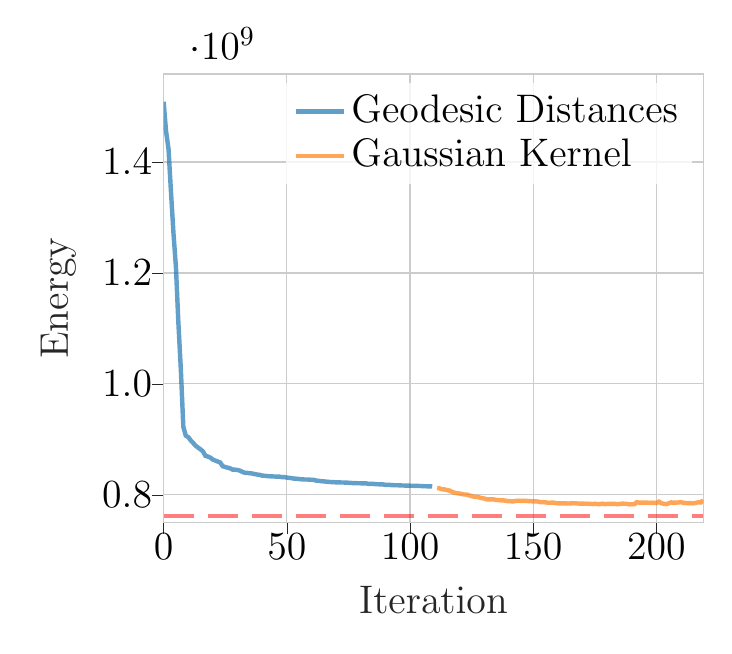
\begin{tikzpicture}

\definecolor{darkorange25512714}{RGB}{255,127,14}
\definecolor{darkslategray38}{RGB}{38,38,38}
\definecolor{lightgray204}{RGB}{204,204,204}
\definecolor{steelblue31119180}{RGB}{31,119,180}

\Large
\begin{axis}[
axis line style={lightgray204},
legend cell align={left},
legend style={fill opacity=0.8, draw opacity=1, text opacity=1, draw=none},
tick align=outside,
tick pos=left,
x grid style={lightgray204},
xlabel=\textcolor{darkslategray38}{Iteration},
xmajorgrids,
xmin=0, xmax=219,
xtick style={color=darkslategray38},
y grid style={lightgray204},
ylabel=\textcolor{darkslategray38}{Energy},
ymajorgrids,
xticklabel style={yshift= 5pt},
yticklabel style={xshift= 5pt},
ymin=550542683.434551037, ymax=1358694122.06139121,
ytick style={color=darkslategray38},
yticklabels={0.4,0.6,0.8,1.0,1.2,1.4,1.6}
]
\addplot [ultra thick, steelblue31119180, opacity=0.7]
table {%
0 1308694122.67322
1 1255134039.19642
2 1223143574.89468
3 1145212342.00702
4 1071660562.52114
5 1010549281.51583
6 909540279.799554
7 825072742.727202
8 722517705.220701
9 706707776.639338
10 703998240.263056
11 698214941.603546
12 693503206.207628
13 688529891.538741
14 685062361.313832
15 682052952.801207
16 678021369.660316
17 670123568.643231
18 669012199.949173
19 667011616.611918
20 663466895.396668
21 661757055.446414
22 660006286.159989
23 658125855.838093
24 651537664.648434
25 650230631.206639
26 648924271.43899
27 647794608.278477
28 645434591.941106
29 645362324.969734
30 644781869.689846
31 643597448.709508
32 641287076.672148
33 639770366.346507
34 639481415.206297
35 638968123.474803
36 638415874.334982
37 637457143.07313
38 636514349.138247
39 636063523.988704
40 634598240.270878
41 634432043.831609
42 633797571.9302
43 633562946.208826
44 633206379.507686
45 633081450.620621
46 632822632.084459
47 632740719.207734
48 632016723.514857
49 631955056.037509
50 631164507.449628
51 630592635.274753
52 630015274.851763
53 629220774.094387
54 629063618.911333
55 628450327.107812
56 628045840.125723
57 627711061.261458
58 627707323.134207
59 627400731.708286
60 627201869.660048
61 627021194.235807
62 625561087.166252
63 625305693.449827
64 624574218.597225
65 624262614.068763
66 623819569.673078
67 623390783.397586
68 623033637.777877
69 622800922.444446
70 622555846.918175
71 622486827.896623
72 622312483.468501
73 622284957.070023
74 622001706.063426
75 621836798.133723
76 621477827.785391
77 621120777.491069
78 621011652.318446
79 620915309.40067
80 620833917.009068
81 620730591.594267
82 620741111.799099
83 619926102.450784
84 619705930.775391
85 619782868.090446
86 619343207.157681
87 619078080.636396
88 618909041.878258
89 618798975.189423
90 618044745.826577
91 617988358.746567
92 617839875.140302
93 617455184.674866
94 617308766.294549
95 617273807.952901
96 617125941.460096
97 616802811.886803
98 616770392.156628
99 616535878.351132
100 616456569.517101
101 616345619.596019
102 616300969.571058
103 616118124.685929
104 615937019.478624
105 615839606.125607
106 615535318.192135
107 615370770.214879
108 615436458.25241
109 615077928.885213
};
\addlegendentry{Geodesic Distances}
\addplot [ultra thick, darkorange25512714, opacity=0.7]
table {%
111 612648372.301906
112 611662205.674109
113 610015170.898197
114 609765111.367364
115 608643620.962938
116 607782890.182881
117 605572518.678166
118 603830782.870329
119 603021851.230176
120 602411377.009876
121 601515259.825287
122 600680106.548735
123 600688145.09389
124 598979294.307838
125 597796863.870596
126 596565066.633388
127 596284372.450001
128 595566341.213237
129 594185609.280201
130 593463916.118725
131 592041568.039415
132 591695059.577726
133 591677157.769964
134 591755925.50642
135 590810755.829279
136 590596877.475266
137 590011242.175887
138 590072535.336405
139 589071941.418743
140 588686442.998376
141 588411728.738422
142 588171047.344407
143 589125737.717016
144 589443632.784902
145 589122400.739687
146 589333318.325826
147 589193788.536528
148 588803128.622151
149 588482574.038744
150 588251629.499683
151 588377677.653596
152 587789202.390581
153 586828313.777811
154 587071861.781051
155 586448515.020599
156 585765021.699341
157 585823464.309016
158 586018138.37902
159 585328574.751973
160 584767511.773227
161 584771092.066519
162 584694431.837749
163 584769694.690591
164 584338693.530078
165 584515805.993903
166 584848676.036812
167 584815992.26678
168 584371937.38755
169 584292312.542714
170 584200089.400307
171 583973664.353263
172 584033204.300175
173 583786553.297186
174 583394360.977737
175 583892638.028153
176 583404843.291737
177 583310188.494599
178 584088049.15557
179 583276014.086446
180 583592940.641809
181 583652702.931611
182 583601291.329494
183 583653176.0634
184 583330123.066812
185 583445946.241169
186 584049156.11105
187 583998672.576763
188 583730160.652931
189 582931472.104415
190 583078961.65941
191 583089180.407408
192 586754756.01036
193 586024426.939826
194 585908209.980571
195 586005037.50462
196 586023762.914037
197 585687205.144002
198 585871595.059091
199 585607281.273647
200 585264662.775361
201 587754137.024738
202 584961281.160602
203 583726839.491549
204 583361301.77597
205 584731186.68361
206 586391797.788864
207 585833866.085215
208 586016205.03599
209 586248894.349355
210 586808952.581457
211 585594315.315987
212 585226482.009306
213 584991869.32544
214 584999533.516353
215 584669305.210516
216 585563585.038832
217 586482905.161003
218 586197157.422245
219 590542683.701471
};
\addlegendentry{Gaussian Kernel}
\path [draw=red, draw opacity=0.5, very thick, dash pattern=on 11.1pt off 4.8pt]
(axis cs:0,561958324.8750211)
--(axis cs:219,561958324.8750211);

\end{axis}

\end{tikzpicture}
}
        \caption{TOSCA}
    \end{subfigure}

        \begin{subfigure}[b]{\linewidth}
    \resizebox{0.49\linewidth}{!}{
    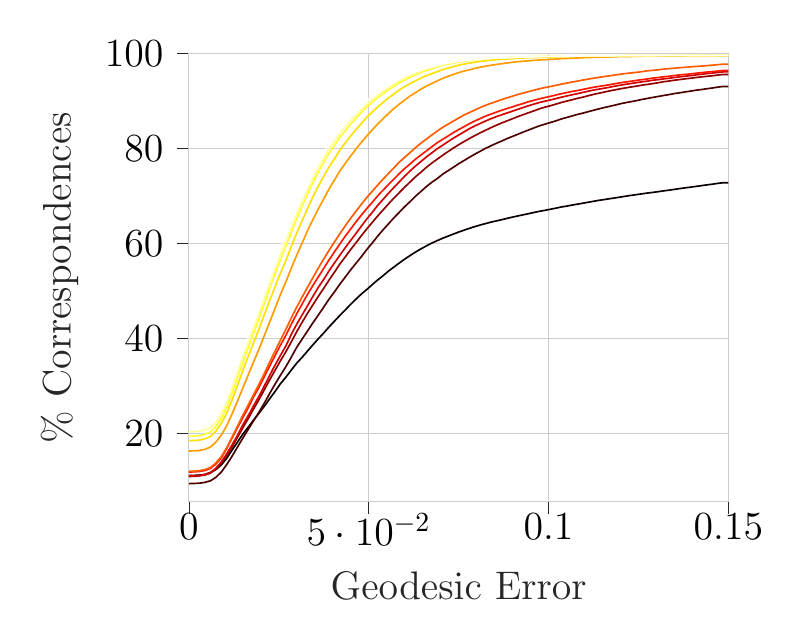
\begin{tikzpicture}

\definecolor{black1000}{RGB}{10,0,0}
\definecolor{darkred14400}{RGB}{144,0,0}
\definecolor{darkslategray38}{RGB}{38,38,38}
\definecolor{gold2552250}{RGB}{255,225,0}
\definecolor{lightgray204}{RGB}{204,204,204}
\definecolor{maroon7600}{RGB}{76,0,0}
\definecolor{orange2551570}{RGB}{255,157,0}
\definecolor{orangered255910}{RGB}{255,91,0}
\definecolor{palegoldenrod255255156}{RGB}{255,255,156}
\definecolor{red21000}{RGB}{210,0,0}
\definecolor{red255230}{RGB}{255,23,0}
\definecolor{yellow25525554}{RGB}{255,255,54}

\Large
\begin{axis}[
axis line style={lightgray204},
tick align=outside,
tick pos=left,
x grid style={lightgray204},
xtick = {0,0.05,0.1,0.15},
xticklabel style={yshift= 5pt},
xlabel=\textcolor{darkslategray38}{Geodesic Error},
xmajorgrids,
xmin=0, xmax=0.15,
xtick style={color=darkslategray38},
y grid style={lightgray204},
ylabel=\textcolor{darkslategray38}{\% Correspondences},
ymajorgrids,
ymin=5.5604249667995, ymax=100,
ytick style={color=darkslategray38}
]
\addplot [semithick, black1000]
table {%
0 11.1111111111111
0.0015 11.1319028609448
0.003 11.1984364604125
0.0045 11.3398203592814
0.006 11.7334774894655
0.0075 12.3281215347084
0.009 13.3025615435795
0.0105 14.6831337325349
0.012 16.4337990685296
0.0135 18.090208471945
0.015 19.8062208915502
0.0165 21.2505544466622
0.018 22.7877578176979
0.0195 24.1946662231093
0.021 25.7027611443779
0.0225 27.2940230649811
0.024 28.8312264360169
0.0255 30.4612996229763
0.027 31.8293967620315
0.0285 33.3264027500554
0.03 34.7762807717897
0.0315 35.9960634286982
0.033 37.3184187181193
0.0345 38.6366156575737
0.036 39.9076846307385
0.0375 41.1219228210246
0.039 42.4123974273675
0.0405 43.6294078509647
0.042 44.8297848746951
0.0435 45.9719449988911
0.045 47.1820248392105
0.0465 48.279829230428
0.048 49.3526835218452
0.0495 50.3021734309159
0.051 51.3140385894877
0.0525 52.2995675316035
0.054 53.1852960745176
0.0555 54.1597360833888
0.057 55.0094255932579
0.0585 55.8632734530938
0.06 56.6713794632956
0.0615 57.4365158571746
0.063 58.1642271013529
0.0645 58.8364936793081
0.066 59.4560878243513
0.0675 60.0576624528721
0.069 60.55666444888
0.0705 61.0722998447549
0.072 61.5061543579508
0.0735 61.9524839210468
0.075 62.3863384342426
0.0765 62.7827677977379
0.078 63.1736526946108
0.0795 63.534043025061
0.081 63.8708693723664
0.0825 64.1813595032158
0.084 64.4835329341317
0.0855 64.738578398758
0.087 65.0005544466622
0.0885 65.273619427811
0.09 65.5411399423375
0.0915 65.789254823686
0.093 66.0318252384121
0.0945 66.2730095364826
0.096 66.5252827677977
0.0975 66.7623087159015
0.099 66.9619095143048
0.1005 67.1975493457529
0.102 67.4123974273675
0.1035 67.6702151253049
0.105 67.8462519405633
0.1065 68.0708028387669
0.108 68.2579285872699
0.1095 68.4575293856731
0.111 68.6654468840097
0.1125 68.8664337990685
0.114 69.071579064094
0.1155 69.2351408294522
0.117 69.419494344644
0.1185 69.5858283433134
0.12 69.767409625194
0.1215 69.9517631403859
0.123 70.1236416056775
0.1245 70.2844311377246
0.126 70.4521512530495
0.1275 70.6073963184742
0.129 70.7460079840319
0.1305 70.8984808161455
0.132 71.067587048126
0.1335 71.2145154136172
0.135 71.3836216455977
0.1365 71.5513417609226
0.138 71.701042359725
0.1395 71.8576735418052
0.141 72.0087602572632
0.1425 72.164005322688
0.144 72.3289532047017
0.1455 72.4675648702595
0.147 72.6422155688623
0.1485 72.7752827677977
0.15 72.7752827677977
};
\addplot [semithick, maroon7600]
table {%
0 9.40064315812819
0.0015 9.42836549123975
0.003 9.49351297405189
0.0045 9.66261920603237
0.006 9.9911288534043
0.0075 10.7022066977157
0.009 11.7958527389665
0.0105 13.3621645597694
0.012 15.1405522288756
0.0135 17.0506209802617
0.015 18.9579174983367
0.0165 20.7972943002883
0.018 22.6311266356177
0.0195 24.4413949878022
0.021 26.3500776225327
0.0225 28.4043025060989
0.024 30.3836770902639
0.0255 32.2410734087381
0.027 34.0485695276114
0.0285 36.0445775116434
0.03 38.1085052117986
0.0315 39.8453093812375
0.033 41.5446884009758
0.0345 43.2620869372366
0.036 44.9032490574407
0.0375 46.5665890441339
0.039 48.2784431137724
0.0405 49.7976269682857
0.042 51.4235418052783
0.0435 52.9080727434021
0.045 54.4300288312265
0.0465 55.839709469949
0.048 57.2299844754935
0.0495 58.7269904635174
0.051 60.0756819693945
0.0525 61.5200155245065
0.054 62.8562319804835
0.0555 64.105123087159
0.057 65.3803504102905
0.0585 66.5446884009758
0.06 67.7284320248392
0.0615 68.7943557329785
0.063 69.9198824573076
0.0645 70.9220447992903
0.066 71.9463850077623
0.0675 72.8418163672655
0.069 73.6235861610113
0.0705 74.5259481037924
0.072 75.2772233311156
0.0735 76.0118651585718
0.075 76.7700709691727
0.0765 77.4492681304059
0.078 78.1326236416056
0.0795 78.7882568196939
0.081 79.4078509647372
0.0825 80.0205145265026
0.084 80.5680306054557
0.0855 81.089210467953
0.087 81.571579064094
0.0885 82.0816699933466
0.09 82.5418607229984
0.0915 82.9992792193391
0.093 83.4677866489244
0.0945 83.9071856287425
0.096 84.3451984919051
0.0975 84.7735085384786
0.099 85.1228099356842
0.1005 85.4610223996452
0.102 85.8020070969173
0.1035 86.1998225770681
0.105 86.5200155245065
0.1065 86.8374362386339
0.108 87.1590153027279
0.1095 87.4320802838767
0.111 87.7439565313817
0.1125 88.0475160789532
0.114 88.3427589265913
0.1155 88.6172100243956
0.117 88.8791860722998
0.1185 89.1453204701707
0.12 89.416999334664
0.1215 89.656797516079
0.123 89.8674872477267
0.1245 90.0823353293413
0.126 90.3318363273453
0.1275 90.5425260589931
0.129 90.7573741406077
0.1305 90.9528165890441
0.132 91.163506320692
0.1335 91.350632069195
0.135 91.5654801508095
0.1365 91.7262696828565
0.138 91.9133954313595
0.1395 92.08250166334
0.141 92.2668551785319
0.1425 92.4123974273675
0.144 92.5787314260368
0.1455 92.7312042581504
0.147 92.9155577733422
0.1485 93.0583277888667
0.15 93.0583277888667
};
\addplot [semithick, darkred14400]
table {%
0 10.9004213794633
0.0015 10.9323020625416
0.003 11.0445775116434
0.0045 11.2275449101796
0.006 11.5962519405633
0.0075 12.4722776668884
0.009 13.6865158571745
0.0105 15.2209469948991
0.012 17.0977489465513
0.0135 19.0854402306498
0.015 21.1327345309381
0.0165 23.0663672654691
0.018 25.1053448658239
0.0195 27.0833333333333
0.021 29.1735972499446
0.0225 31.2846529163894
0.024 33.3000665335995
0.0255 35.3127079174983
0.027 37.1839654025283
0.0285 39.2589820359281
0.03 41.3936016855179
0.0315 43.3715901530273
0.033 45.2705699711688
0.0345 47.0586604568641
0.036 48.8439787092482
0.0375 50.5267243291195
0.039 52.2981814149479
0.0405 53.9337990685296
0.042 55.6650587713462
0.0435 57.1551341760923
0.045 58.7089709469949
0.0465 60.1519183854513
0.048 61.6461521401641
0.0495 63.071080062098
0.051 64.416999334664
0.0525 65.7698491905079
0.054 67.0395320470171
0.0555 68.3050565535595
0.057 69.5470170769572
0.0585 70.6822466178754
0.06 71.8465846085606
0.0615 72.9208250166334
0.063 74.0338766910623
0.0645 74.9722776668884
0.066 75.9924595253936
0.0675 76.8878908848969
0.069 77.7070858283433
0.0705 78.5290530051009
0.072 79.3052783322244
0.0735 80.0745730760701
0.075 80.7717897538257
0.0765 81.4412840984697
0.078 82.0830561100022
0.0795 82.7165114216013
0.081 83.2889776003548
0.0825 83.836493679308
0.084 84.3826236416057
0.0855 84.8885562208915
0.087 85.3778554003105
0.0885 85.8227988467509
0.09 86.2621978265691
0.0915 86.7223885562209
0.093 87.1312929696163
0.0945 87.5443557329785
0.096 87.9338545131958
0.0975 88.3607784431138
0.099 88.7031492570415
0.1005 88.9928476380572
0.102 89.3296739853625
0.1035 89.6706586826347
0.105 89.9686737635839
0.1065 90.2472832113551
0.108 90.5508427589266
0.1095 90.798957640275
0.111 91.1039033045021
0.1125 91.3838988689288
0.114 91.6375582168995
0.1155 91.8759702816589
0.117 92.1310157462852
0.1185 92.3444777112442
0.12 92.5759591927257
0.1215 92.7714016411621
0.123 92.9571412730096
0.1245 93.1345642049235
0.126 93.3369372366378
0.1275 93.500499001996
0.129 93.6654468840098
0.1305 93.8470281658904
0.132 94.061876247505
0.1335 94.2060323796851
0.135 94.3792969616323
0.1365 94.5123641605678
0.138 94.6703814593036
0.1395 94.7868152583722
0.141 94.9489909070748
0.1425 95.0806719893546
0.144 95.1915613218008
0.1455 95.3066090042138
0.147 95.4576957196718
0.1485 95.5810601020182
0.15 95.5810601020182
};
\addplot [semithick, red21000]
table {%
0 10.9905189620758
0.0015 11.0126968285651
0.003 11.1152694610778
0.0045 11.2816034597472
0.006 11.7196163229097
0.0075 12.6164337990685
0.009 13.9290862719006
0.0105 15.6270791749834
0.012 17.5205145265025
0.0135 19.5068196939454
0.015 21.7329230428033
0.0165 23.6831891772011
0.018 25.7900864936793
0.0195 27.763916611222
0.021 29.983089376802
0.0225 32.211964958971
0.024 34.3840097582612
0.0255 36.4313040585496
0.027 38.4231536926148
0.0285 40.8322244400089
0.03 42.9668440895986
0.0315 44.9365158571745
0.033 46.8576735418053
0.0345 48.8439787092482
0.036 50.7554335772899
0.0375 52.4062985140829
0.039 54.2359724994456
0.0405 55.8993124861388
0.042 57.5155245065425
0.0435 59.0915391439344
0.045 60.6412175648703
0.0465 62.1229762696829
0.048 63.6643379906853
0.0495 65.1668884453315
0.051 66.521124417831
0.0525 68.0070414726104
0.054 69.2656353958749
0.0555 70.5574961188734
0.057 71.7675759591927
0.0585 72.9485473497449
0.06 74.1475382568197
0.0615 75.2453426480373
0.063 76.2863162563762
0.0645 77.2205588822355
0.066 78.1783654912397
0.0675 79.0433022843202
0.069 79.8971501441561
0.0705 80.6456531381681
0.072 81.4052450654247
0.0735 82.1412730095365
0.075 82.8149257041473
0.0765 83.4830339321357
0.078 84.1553005100909
0.0795 84.7485584386782
0.081 85.2586493679308
0.0825 85.7839875803948
0.084 86.2608117099135
0.0855 86.7015968063872
0.087 87.0938678199158
0.0885 87.4847527167886
0.09 87.8659347970726
0.0915 88.2568196939454
0.093 88.6282989576403
0.0945 89.0136393878909
0.096 89.354624085163
0.0975 89.6886781991572
0.099 89.9534264803726
0.1005 90.2140164116212
0.102 90.4953980927035
0.1035 90.7864825903748
0.105 91.0443002883123
0.1065 91.3021179862497
0.108 91.5363717010423
0.1095 91.7955755156354
0.111 92.0575515635396
0.1125 92.3001219782657
0.114 92.4983366600133
0.1155 92.689620758483
0.117 92.9044688400976
0.1185 93.135950321579
0.12 93.3244621867376
0.1215 93.526835218452
0.123 93.6903969838102
0.1245 93.874750499002
0.126 94.0341539143934
0.1275 94.1893989798182
0.129 94.37375249501
0.1305 94.4971168773564
0.132 94.6537480594367
0.1335 94.7812707917498
0.135 94.9462186737636
0.1365 95.0917609225992
0.138 95.2192836549124
0.1395 95.3468063872255
0.141 95.4951208693723
0.1425 95.6365047682413
0.144 95.7709580838323
0.1455 95.8776890663118
0.147 96.0065979152805
0.1485 96.1271900643158
0.15 96.1271900643158
};
\addplot [semithick, red255230]
table {%
0 11.8512974051896
0.0015 11.8693169217121
0.003 11.9580283876691
0.0045 12.1645597693502
0.006 12.5970281658904
0.0075 13.4896872920825
0.009 14.7676868485252
0.0105 16.7318141494788
0.012 18.9551452650255
0.0135 21.1327345309381
0.015 23.2673541805278
0.0165 25.3451430472389
0.018 27.6350077622533
0.0195 29.6864604125083
0.021 31.9250388112664
0.0225 34.1774783765802
0.024 36.3911066755378
0.0255 38.5922599245953
0.027 40.6409403415391
0.0285 42.9737746728765
0.03 45.1693834553116
0.0315 47.2305389221557
0.033 49.2459525393657
0.0345 51.1269128409847
0.036 52.9468840097583
0.0375 54.7252716788645
0.039 56.5327677977379
0.0405 58.2238301175427
0.042 59.8927145708583
0.0435 61.5255599911289
0.045 63.0267243291196
0.0465 64.568086050122
0.048 65.9833111554669
0.0495 67.3624972277667
0.051 68.6585163007318
0.0525 70.023841206476
0.054 71.2131292969617
0.0555 72.4107340873808
0.057 73.5223996451542
0.0585 74.6950543357729
0.06 75.7651363938789
0.0615 76.7284874695054
0.063 77.7417387447328
0.0645 78.6011310711909
0.066 79.4646817476159
0.0675 80.3199157241073
0.069 81.1751497005988
0.0705 81.8987025948103
0.072 82.5903748059437
0.0735 83.3097693501885
0.075 83.9695608782435
0.0765 84.5794522066977
0.078 85.2156797516079
0.0795 85.7853736970504
0.081 86.3037813262364
0.0825 86.813872255489
0.084 87.2338656021291
0.0855 87.6552450654247
0.087 88.0544466622311
0.0885 88.409292526059
0.09 88.7752273231316
0.0915 89.1453204701708
0.093 89.4724440008871
0.0945 89.8577844311377
0.096 90.165502328676
0.0975 90.4538145930362
0.099 90.736582390774
0.1005 90.9791528055001
0.102 91.2480594366822
0.1035 91.5225105344866
0.105 91.7692392991794
0.1065 92.0062652472832
0.108 92.1947771124418
0.1095 92.4318030605456
0.111 92.6605123087159
0.1125 92.8878354402306
0.114 93.0680306054558
0.1155 93.2482257706808
0.117 93.4353515191838
0.1185 93.6474273674872
0.12 93.8359392326458
0.1215 94.0161343978709
0.123 94.1741516966068
0.1245 94.3460301618984
0.126 94.5026613439787
0.1275 94.6357285429141
0.129 94.8173098247948
0.1305 94.9462186737636
0.132 95.095919272566
0.1335 95.2165114216012
0.135 95.3634397870924
0.1365 95.4965069860279
0.138 95.6004657351962
0.1395 95.7168995342648
0.141 95.8444222665779
0.1425 95.9719449988911
0.144 96.0939232645819
0.1455 96.1964958970947
0.147 96.2976824129519
0.1485 96.4196606786427
0.15 96.4196606786427
};
\addplot [semithick, orangered255910]
table {%
0 12.0051563539587
0.0015 12.0328786870703
0.003 12.1202040363717
0.0045 12.3544577511643
0.006 12.785540031049
0.0075 13.7378021734309
0.009 15.0532268795742
0.0105 16.9023064981149
0.012 19.1367265469062
0.0135 21.4321357285429
0.015 23.7455644267021
0.0165 25.9314703925482
0.018 28.138168108228
0.0195 30.2852628077179
0.021 32.6014637391883
0.0225 35.0202373031714
0.024 37.3378243512974
0.0255 39.6914504324684
0.027 41.8939897981814
0.0285 44.3002883122644
0.03 46.5624306941672
0.0315 48.6776447105788
0.033 50.7692947438456
0.0345 52.7722333111555
0.036 54.8098247948547
0.0375 56.6852406298514
0.039 58.5662009314704
0.0405 60.3057773342204
0.042 62.0342648037259
0.0435 63.7142381902861
0.045 65.3041139942337
0.0465 66.8011199822577
0.048 68.2690175205145
0.0495 69.6884009758261
0.051 70.9747172322022
0.0525 72.2818252384121
0.054 73.5279441117764
0.0555 74.7352517187846
0.057 75.9079064094034
0.0585 77.1166001330672
0.06 78.1353958749169
0.0615 79.1278554003105
0.063 80.1480372588157
0.0645 81.1030716345088
0.066 81.9444444444444
0.0675 82.7969061876247
0.069 83.6285761809714
0.0705 84.4186626746507
0.072 85.083998669328
0.0735 85.7465624306942
0.075 86.3980372588157
0.0765 87.0453537369705
0.078 87.562375249501
0.0795 88.0918718119317
0.081 88.6185961410513
0.0825 89.0981925038811
0.084 89.5084830339322
0.0855 89.8924373475272
0.087 90.3027278775782
0.0885 90.6700487913062
0.09 91.022122421823
0.0915 91.3741960523398
0.093 91.6763694832557
0.0945 91.9840873807939
0.096 92.2779441117764
0.0975 92.5773453093812
0.099 92.831004657352
0.1005 93.0486249722777
0.102 93.2939676203149
0.1035 93.5393102683522
0.105 93.7416833000666
0.1065 93.9870259481038
0.108 94.1810822798847
0.1095 94.4042470614327
0.111 94.6149367930805
0.1125 94.7951319583056
0.114 94.9753271235307
0.1155 95.1485917054779
0.117 95.3010645375915
0.1185 95.4826458194722
0.12 95.6420492348636
0.1215 95.7903637170104
0.123 95.9123419827013
0.1245 96.0398647150144
0.126 96.1812486138833
0.1275 96.3558993124862
0.129 96.4598580616544
0.1305 96.5707473941007
0.132 96.7162896429363
0.1335 96.8188622754491
0.135 96.9117320913728
0.1365 97.0087602572633
0.138 97.0946994899091
0.1395 97.1986582390774
0.141 97.2748946551342
0.1425 97.3552894211577
0.144 97.4453870037702
0.1455 97.5424151696607
0.147 97.646373918829
0.1485 97.7461743180306
0.15 97.7461743180306
};
\addplot [semithick, orange2551570]
table {%
0 16.2743956531382
0.0015 16.297959636283
0.003 16.38667110224
0.0045 16.6250831669993
0.006 17.0838877799956
0.0075 18.1179308050566
0.009 19.5594921268574
0.0105 21.540252827678
0.012 24.001996007984
0.0135 26.7104679529829
0.015 29.5076513639388
0.0165 32.2729540918164
0.018 35.0049900199601
0.0195 37.6898979818141
0.021 40.5785650920381
0.0225 43.4603016189842
0.024 46.3642160124196
0.0255 49.2764471057884
0.027 51.926702151253
0.0285 54.7987358616101
0.03 57.516910623198
0.0315 60.057662452872
0.033 62.6663339986693
0.0345 65.0296628964294
0.036 67.2710135284986
0.0375 69.3695941450432
0.039 71.4654025282768
0.0405 73.3643823464183
0.042 75.2619760479042
0.0435 76.8684852517188
0.045 78.4209359059658
0.0465 79.9110113107119
0.048 81.3026724329119
0.0495 82.6513639387891
0.051 83.9085717453981
0.0525 85.1477600354846
0.054 86.2829895764028
0.0555 87.3641605677534
0.057 88.3982035928144
0.0585 89.318585052118
0.06 90.1876801951652
0.0615 91.0443002883123
0.063 91.7609225992459
0.0645 92.4858616101131
0.066 93.1207030383677
0.0675 93.661288534043
0.069 94.2157351962741
0.0705 94.7396872920825
0.072 95.1763140385895
0.0735 95.5866045686405
0.075 95.9650144156132
0.0765 96.3059991128853
0.078 96.566589044134
0.0795 96.8604457751164
0.081 97.1141051230872
0.0825 97.3358837879796
0.084 97.5202373031714
0.0855 97.6976602350854
0.087 97.8556775338213
0.0885 98.0067642492792
0.09 98.1523064981149
0.0915 98.2784431137725
0.093 98.3810157462852
0.0945 98.4711133288978
0.096 98.5598247948547
0.0975 98.6429917941894
0.099 98.6970503437569
0.1005 98.778831226436
0.102 98.8384342426259
0.1035 98.913284542027
0.105 98.9534819250388
0.1065 99.0130849412287
0.108 99.0615990241739
0.1095 99.117043690397
0.111 99.1558549567532
0.1125 99.1877356398315
0.114 99.2251607895321
0.1155 99.2570414726104
0.117 99.2847638057219
0.1185 99.3221889554225
0.12 99.3526835218452
0.1215 99.3679308050565
0.123 99.3845642049234
0.1245 99.4053559547571
0.126 99.4344644045242
0.1275 99.4497116877356
0.129 99.4635728542914
0.1305 99.4871368374362
0.132 99.5051563539587
0.1335 99.5176314038589
0.135 99.5356509203814
0.1365 99.5411953870037
0.138 99.5453537369705
0.1395 99.5550565535595
0.141 99.5578287868707
0.1425 99.5675316034597
0.144 99.5703038367709
0.1455 99.5786205367043
0.147 99.5800066533599
0.1485 99.5855511199822
0.15 99.5855511199822
};
\addplot [semithick, gold2552250]
table {%
0 18.447826569084
0.0015 18.4727766688844
0.003 18.5739631847416
0.0045 18.8359392326458
0.006 19.3169217121313
0.0075 20.4050232867598
0.009 22.0447992903083
0.0105 24.1821911732091
0.012 26.9807607008206
0.0135 30.0329895764027
0.015 33.1392770015525
0.0165 36.1554668440896
0.018 39.0316589044134
0.0195 41.9383455311599
0.021 45.016910623198
0.0225 47.9873586161011
0.024 50.8885007762253
0.0255 53.7771678864493
0.027 56.4218784652916
0.0285 59.3299512086937
0.03 62.1895098691506
0.0315 64.7773896651142
0.033 67.315369261477
0.0345 69.8089931248614
0.036 72.0170769571967
0.0375 74.1281326236416
0.039 76.1102794411178
0.0405 77.8110445775116
0.042 79.6490352628077
0.0435 81.1903969838102
0.045 82.6430472388556
0.0465 83.9958970946995
0.048 85.2808272344201
0.0495 86.581004657352
0.051 87.7009869150588
0.0525 88.7170104235972
0.054 89.7261033488578
0.0555 90.6423264581947
0.057 91.4545908183633
0.0585 92.3070525615436
0.06 93.0250609891328
0.0615 93.6585163007319
0.063 94.2351408294522
0.0645 94.8186959414504
0.066 95.3371035706365
0.0675 95.7376912840985
0.069 96.1798624972277
0.0705 96.5804502106897
0.072 96.9158904413395
0.0735 97.2222222222222
0.075 97.5521179862497
0.0765 97.7794411177644
0.078 97.9776557995121
0.0795 98.1564648480816
0.081 98.3214127300954
0.0825 98.4766577955201
0.084 98.5861610113107
0.0855 98.7039809270348
0.087 98.7857618097139
0.0885 98.8481370592149
0.09 98.9326901752051
0.0915 99.0172432911954
0.093 99.064371257485
0.0945 99.1239742736748
0.096 99.1572410734087
0.0975 99.189121756487
0.099 99.2223885562209
0.1005 99.2598137059215
0.102 99.3013972055888
0.1035 99.3332778886671
0.105 99.3554557551564
0.1065 99.3748613883345
0.108 99.3970392548237
0.1095 99.4095143047239
0.111 99.419217121313
0.1125 99.4372366378355
0.114 99.4497116877357
0.1155 99.4608006209803
0.117 99.4760479041916
0.1185 99.4829784874695
0.12 99.4982257706809
0.1215 99.5093147039255
0.123 99.5120869372366
0.1245 99.5176314038589
0.126 99.5342648037259
0.1275 99.5384231536926
0.129 99.5453537369705
0.1305 99.5522843202484
0.132 99.5564426702151
0.1335 99.5578287868707
0.135 99.5606010201818
0.1365 99.5606010201818
0.138 99.5647593701486
0.1395 99.5772344200488
0.141 99.5786205367044
0.1425 99.5827788866711
0.144 99.5869372366378
0.1455 99.589709469949
0.147 99.5924817032601
0.1485 99.5952539365713
0.15 99.5952539365713
};
\addplot [semithick, yellow25525554]
table {%
0 19.3959303614992
0.0015 19.4167221113329
0.003 19.5123641605677
0.0045 19.7784985584387
0.006 20.3010645375915
0.0075 21.4099578620537
0.009 23.1412175648703
0.0105 25.383954313595
0.012 28.4167775559991
0.0135 31.6672211133289
0.015 34.887170104236
0.0165 38.0322687957419
0.018 41.0831115546684
0.0195 44.1422710135285
0.021 47.3275670880461
0.0225 50.4962297626968
0.024 53.6454868041694
0.0255 56.5993013972056
0.027 59.4491572410734
0.0285 62.3253493013972
0.03 65.2098580616545
0.0315 67.8032823242404
0.033 70.3523508538479
0.0345 72.8043912175649
0.036 75.0180195165225
0.0375 77.0500665335995
0.039 79.0044910179641
0.0405 80.6207030383677
0.042 82.3533488578399
0.0435 83.7436238633844
0.045 85.1269682856509
0.0465 86.367542692393
0.048 87.615047682413
0.0495 88.757207806609
0.051 89.7801618984254
0.0525 90.6922266577955
0.054 91.5557773342204
0.0555 92.3541805278332
0.057 93.0791195387004
0.0585 93.7957418496341
0.06 94.4139498780217
0.0615 94.9794854734974
0.063 95.506209802617
0.0645 96.0093701485917
0.066 96.4141162120204
0.0675 96.7703481925039
0.069 97.1390552228876
0.0705 97.4717232202262
0.072 97.7503326679973
0.0735 97.9637946329563
0.075 98.1925038811266
0.0765 98.3837879795963
0.078 98.5168551785319
0.0795 98.6526946107785
0.081 98.7566533599468
0.0825 98.8619982257706
0.084 98.9423929917942
0.0855 99.0130849412286
0.087 99.0615990241739
0.0885 99.1017964071856
0.09 99.1572410734087
0.0915 99.2126857396319
0.093 99.268130405855
0.0945 99.3041694389
0.096 99.3429807052562
0.0975 99.3776336216456
0.099 99.402583721446
0.1005 99.419217121313
0.102 99.4538700377024
0.1035 99.4788201375028
0.105 99.491295187403
0.1065 99.4982257706808
0.108 99.5065424706143
0.1095 99.5162452872033
0.111 99.5190175205145
0.1125 99.527334220448
0.114 99.5342648037259
0.1155 99.5425815036593
0.117 99.5495120869372
0.1185 99.5550565535595
0.12 99.5606010201819
0.1215 99.5689177201153
0.123 99.5716899534265
0.1245 99.5772344200488
0.126 99.5841650033266
0.1275 99.5883233532934
0.129 99.589709469949
0.1305 99.599412286538
0.132 99.599412286538
0.1335 99.6007984031936
0.135 99.6007984031936
0.1365 99.6021845198492
0.138 99.6035706365048
0.1395 99.6035706365048
0.141 99.6049567531603
0.1425 99.6049567531603
0.144 99.6049567531603
0.1455 99.6063428698159
0.147 99.6091151031271
0.1485 99.6091151031271
0.15 99.6091151031271
};
\addplot [semithick, palegoldenrod255255156]
table {%
0 20.3357174539809
0.0015 20.355123087159
0.003 20.4452206697716
0.0045 20.7044244843646
0.006 21.2172876469284
0.0075 22.3372699046352
0.009 24.0962519405633
0.0105 26.408294522067
0.012 29.4688400975826
0.0135 32.8107673541805
0.015 36.0501219782657
0.0165 39.09542027057
0.018 42.171213129297
0.0195 45.1763140385895
0.021 48.4142825460191
0.0225 51.5316589044134
0.024 54.6878465291639
0.0255 57.7068086050122
0.027 60.5012197826569
0.0285 63.3164227101353
0.03 66.2078620536704
0.0315 68.7694056331781
0.033 71.3143158128188
0.0345 73.75249500998
0.036 75.9633510756265
0.0375 77.9995564426702
0.039 79.9484364604125
0.0405 81.4870259481038
0.042 83.19333555112
0.0435 84.5545021068973
0.045 85.8824018629408
0.0465 87.0508982035928
0.048 88.1972166777556
0.0495 89.3158128188068
0.051 90.3193612774451
0.0525 91.2064759370149
0.054 92.0256708804613
0.0555 92.7838766910623
0.057 93.5240629851408
0.0585 94.2074184963407
0.06 94.8186959414504
0.0615 95.3592814371258
0.063 95.8250166333999
0.0645 96.300454646263
0.066 96.6968840097582
0.0675 97.0018296739854
0.069 97.334497671324
0.0705 97.6297405189621
0.072 97.8903304502107
0.0735 98.1065646484808
0.075 98.3172543801286
0.0765 98.4822022621424
0.078 98.6000221778665
0.0795 98.7289310268352
0.081 98.8287314260368
0.0825 98.913284542027
0.084 98.9978376580173
0.0855 99.0463517409625
0.087 99.0962519405633
0.0885 99.1309048569528
0.09 99.1932801064538
0.0915 99.2320913728099
0.093 99.2681304058549
0.0945 99.3152583721446
0.096 99.3415945886006
0.0975 99.366544688401
0.099 99.392880904857
0.1005 99.4067420714127
0.102 99.4413949878021
0.1035 99.4663450876025
0.105 99.4802062541583
0.1065 99.4940674207141
0.108 99.4996118873364
0.1095 99.5093147039254
0.111 99.5120869372366
0.1125 99.5162452872033
0.114 99.527334220448
0.1155 99.5356509203814
0.117 99.5508982035928
0.1185 99.5564426702151
0.12 99.5592149035262
0.1215 99.5689177201153
0.123 99.573076070082
0.1245 99.5786205367043
0.126 99.5869372366378
0.1275 99.5910955866046
0.129 99.5938678199157
0.1305 99.6021845198492
0.132 99.6021845198492
0.1335 99.6105012197826
0.135 99.6118873364382
0.1365 99.6118873364382
0.138 99.6118873364382
0.1395 99.6132734530938
0.141 99.6132734530938
0.1425 99.6132734530938
0.144 99.6174318030605
0.1455 99.6174318030605
0.147 99.6188179197161
0.1485 99.6188179197161
0.15 99.6188179197161
};
\addplot [semithick, white]
table {%
0 21.2699600798403
0.0015 21.2893657130184
0.003 21.38916611222
0.0045 21.6372809935684
0.006 22.1432135728543
0.0075 23.3075515635396
0.009 25.1136615657574
0.0105 27.4728321135507
0.012 30.6082279884675
0.0135 33.9640164116212
0.015 37.2491128853404
0.0165 40.3456974939011
0.018 43.4214903526281
0.0195 46.4390663118208
0.021 49.7699046351741
0.0225 52.9219339099578
0.024 56.0808937680195
0.0255 59.0097582612553
0.027 61.8263473053892
0.0285 64.6997671324019
0.03 67.5399201596806
0.0315 69.9656243069417
0.033 72.4675648702595
0.0345 74.9057440674207
0.036 77.051452650255
0.0375 78.9989465513418
0.039 80.9256487025948
0.0405 82.4725548902196
0.042 84.1317365269461
0.0435 85.4624085163007
0.045 86.7501108893324
0.0465 87.8964293634952
0.048 88.9457196717676
0.0495 90.0116433799068
0.051 90.9930139720559
0.0525 91.8510201818585
0.054 92.6203149257042
0.0555 93.3785207363052
0.057 94.0272233311155
0.0585 94.6620647593702
0.06 95.2442337547128
0.0615 95.7515524506542
0.063 96.1854069638501
0.0645 96.5721335107563
0.066 96.9560878243513
0.0675 97.2263805721889
0.069 97.5340984697272
0.0705 97.7988467509425
0.072 98.0233976491462
0.0735 98.207751164338
0.075 98.3782435129741
0.0765 98.5431913949878
0.078 98.6416056775338
0.0795 98.7552672432912
0.081 98.8536815258372
0.0825 98.9340762918607
0.084 99.0033821246396
0.0855 99.0588267908627
0.087 99.1045686404968
0.0885 99.1309048569528
0.09 99.1780328232424
0.0915 99.225160789532
0.093 99.2598137059215
0.0945 99.2972388556221
0.096 99.3194167221113
0.0975 99.349911288534
0.099 99.3748613883344
0.1005 99.3928809048569
0.102 99.4164448880017
0.1035 99.4469394544245
0.105 99.464958970947
0.1065 99.4774340208472
0.108 99.4843646041251
0.1095 99.4926813040585
0.111 99.500998003992
0.1125 99.5134730538922
0.114 99.5231758704812
0.1155 99.5328786870703
0.117 99.5425815036593
0.1185 99.5453537369705
0.12 99.5522843202483
0.1215 99.5578287868707
0.123 99.5675316034597
0.1245 99.5703038367709
0.126 99.5800066533599
0.1275 99.5827788866711
0.129 99.589709469949
0.1305 99.5952539365713
0.132 99.5980261698824
0.1335 99.6021845198492
0.135 99.6021845198492
0.1365 99.6021845198492
0.138 99.6021845198492
0.1395 99.6035706365047
0.141 99.6049567531603
0.1425 99.6049567531603
0.144 99.6049567531603
0.1455 99.6077289864715
0.147 99.6077289864715
0.1485 99.6091151031271
0.15 99.6091151031271
};
\end{axis}

\end{tikzpicture}
}
    \resizebox{0.463\linewidth}{!}{
    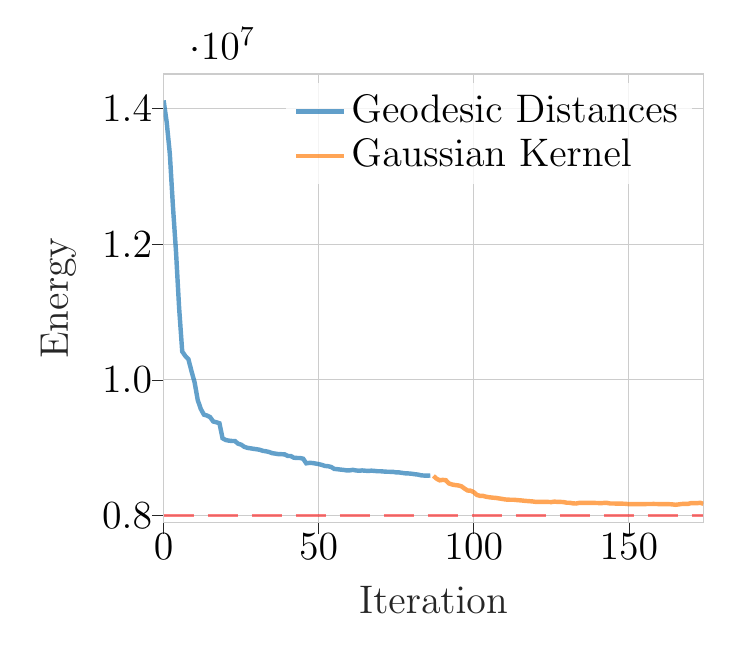
\begin{tikzpicture}

\definecolor{darkorange25512714}{RGB}{255,127,14}
\definecolor{darkslategray38}{RGB}{38,38,38}
\definecolor{lightgray204}{RGB}{204,204,204}
\definecolor{steelblue31119180}{RGB}{31,119,180}

\Large
\begin{axis}[
axis line style={lightgray204},
legend cell align={left},
legend style={fill opacity=0.8, draw opacity=1, text opacity=1, draw=none},
tick align=outside,
tick pos=left,
x grid style={lightgray204},
xlabel=\textcolor{darkslategray38}{Iteration},
xmajorgrids,
xmin=0, xmax=174,
xtick style={color=darkslategray38},
xtick={0,50,100,150},
y grid style={lightgray204},
ylabel=\textcolor{darkslategray38}{Energy},
ymajorgrids,
xticklabel style={yshift= 5pt},
yticklabel style={xshift= 5pt},
ymin=11899175.434551037, ymax=18512179.06139121,
ytick style={color=darkslategray38},
yticklabels={0.4,0.6,0.8,1.0,1.2,1.4,1.6}
]
\addplot [ultra thick, steelblue31119180, opacity=0.7]
table {%
0 18122179.8669987
1 17798598.3730782
2 17336005.1639099
3 16565909.8601921
4 15887572.0343383
5 15060570.0062235
6 14418579.5084637
7 14352494.8399955
8 14304678.1541237
9 14125914.9140919
10 13962793.9564897
11 13702388.304692
12 13570296.7785852
13 13487029.0765126
14 13473959.336156
15 13450187.8127192
16 13386065.2981522
17 13374884.0466379
18 13360185.2965563
19 13138836.069291
20 13113510.5345848
21 13103944.2723291
22 13098748.4271311
23 13098189.4844467
24 13059058.5748893
25 13044477.6776274
26 13013300.9280487
27 12997610.0498212
28 12990455.8789019
29 12983247.5432979
30 12976661.7930118
31 12969046.3110918
32 12953556.3152338
33 12946624.421873
34 12936175.2850095
35 12919247.2335172
36 12912272.2179775
37 12904967.2091222
38 12903576.5460348
39 12901286.8466065
40 12878229.5909736
41 12876444.4885278
42 12851921.5565257
43 12848209.7258882
44 12847648.6106095
45 12836721.3261999
46 12769279.6355737
47 12775831.4618156
48 12773918.4500608
49 12765782.4750709
50 12757603.4901589
51 12746119.2546517
52 12730557.7945106
53 12726601.1047852
54 12715806.5118059
55 12687134.5579642
56 12682547.0364317
57 12676958.5786945
58 12672506.4689028
59 12664773.8833204
60 12665280.4519888
61 12672748.575727
62 12664385.8700152
63 12659464.1963306
64 12664280.8741793
65 12660394.6615701
66 12656404.1785754
67 12661052.2751021
68 12657224.4543779
69 12652347.1963262
70 12652090.7819975
71 12648035.6510842
72 12644967.5809122
73 12644268.8623104
74 12643161.6593385
75 12635126.8284286
76 12634425.0718222
77 12627546.7113692
78 12621055.805236
79 12619516.5889837
80 12615320.2847639
81 12608362.5930857
82 12603123.1146949
83 12591840.9369272
84 12588683.0306296
85 12586683.6923936
86 12590342.6964495
};
\addlegendentry{Geodesic Distances}
\addplot [ultra thick, darkorange25512714, opacity=0.7]
table {%
87 12583387.277718
88 12542999.4465372
89 12518474.5297786
90 12524955.0759853
91 12519876.5330193
92 12472696.2763353
93 12456960.2232831
94 12448596.19386
95 12443230.7195219
96 12430795.5521528
97 12397623.5076284
98 12368280.3529401
99 12365248.0556883
100 12343671.023693
101 12303197.4275818
102 12289659.6883343
103 12288461.7572656
104 12276455.6970974
105 12268666.3932064
106 12262701.0959159
107 12259737.4622653
108 12252427.017184
109 12245204.588397
110 12237265.4480939
111 12232832.818362
112 12232059.8829914
113 12231748.8493207
114 12226514.9965066
115 12223080.8072794
116 12218360.1126516
117 12213862.4189998
118 12210566.1962907
119 12206843.1582104
120 12200425.6031285
121 12200254.8458254
122 12200100.6554202
123 12199639.7221578
124 12199562.069871
125 12197324.7456874
126 12204193.3926257
127 12200508.4215749
128 12199846.3280101
129 12197228.3270102
130 12188020.4954249
131 12186942.3049936
132 12178355.7806965
133 12176187.89913
134 12185860.036086
135 12185755.2171826
136 12184769.1192064
137 12186384.7033895
138 12184634.3986512
139 12184876.188495
140 12183592.6457171
141 12181556.2298388
142 12185036.2546158
143 12185017.2513453
144 12176382.2081102
145 12177028.749105
146 12175184.8693114
147 12173797.7727082
148 12173678.6278561
149 12172058.3039014
150 12166621.8888097
151 12166822.8893195
152 12166654.3670695
153 12166344.8847359
154 12166489.7970455
155 12167219.3556666
156 12169358.5142826
157 12169368.6820421
158 12169864.7808969
159 12169244.87127
160 12167426.742234
161 12166656.7228009
162 12166626.7213735
163 12166270.2589766
164 12164082.2880854
165 12157667.3197123
166 12162859.6349452
167 12169564.4856691
168 12170444.0432437
169 12169781.648779
170 12181184.3464855
171 12183398.99473
172 12181501.4735145
173 12187109.7056383
174 12172671.1344483
};
\addlegendentry{Gaussian Kernel}
\path [draw=red, draw opacity=0.5, very thick, dash pattern=on 11.1pt off 4.8pt]
(axis cs:0,11999175.853289634)
--(axis cs:174,11999175.853289634);

\end{axis}

\end{tikzpicture}
}
        \caption{SMAL}
    \end{subfigure}

    \caption{Evolution during the optimisation (left) of the PCK, depicted with a colour bar gradient, and (right) of the total  energy. 
    The horizontal red-dashed line is the energy of the ground-truth solution. 
    The results are on (a)  a class of FAUST containing ten shapes, (b) the cat class of TOSCA containing eleven shapes, and (c) the cat class of SMAL containing nine shapes. 
    }
    \label{fig:Improvement}
\end{figure}



\section{Fixed Anchor vs. Random Triplets}\label{sec:anchorchoice}

Fig.~\ref{fig:AnchorAblation} compares our anchor-based scheme with using random triplets. 
We see a small improvement with our scheme. 

\begin{figure}%
    \centering
    \resizebox{0.59 \linewidth}{!}{
    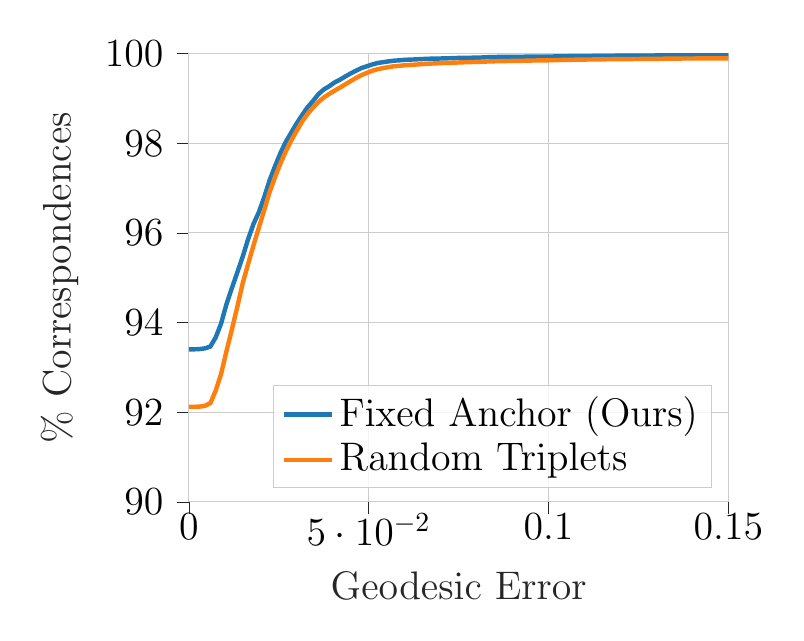
\begin{tikzpicture}

\definecolor{darkorange25512714}{RGB}{255,127,14}
\definecolor{darkslategray38}{RGB}{38,38,38}
\definecolor{lightgray204}{RGB}{204,204,204}
\definecolor{steelblue31119180}{RGB}{31,119,180}

\Large
\begin{axis}[
axis line style={lightgray204},
legend cell align={left},
legend style={fill opacity=0.8, draw opacity=1, text opacity=1, draw=lightgray204, anchor=south east,at={(0.97,0.03)}},
tick align=outside,
tick pos=left,
xtick = {0,0.05,0.1,0.15},
x grid style={lightgray204},
xlabel=\textcolor{darkslategray38}{Geodesic Error},
xmajorgrids,
xmin=0, xmax=0.15,
xtick style={color=darkslategray38},
xticklabel style={yshift= 5pt},
y grid style={lightgray204},
ylabel=\textcolor{darkslategray38}{\% Correspondences},
ymajorgrids,
ymin=90, ymax=100,
ytick style={color=darkslategray38}
]
\addplot [ultra thick, steelblue31119180]
table {%
0 93.4019477644976
0.0015 93.4021691013723
0.003 93.4074811863656
0.0045 93.4229747675963
0.006 93.4645861000443
0.0075 93.6702080566622
0.009 93.9803010181496
0.0105 94.4156706507304
0.012 94.7726870296591
0.0135 95.1188579017264
0.015 95.4712262062859
0.0165 95.8612217795485
0.018 96.199203187251
0.0195 96.4645861000443
0.021 96.8025675077468
0.0225 97.1790615316512
0.024 97.4922532093847
0.0255 97.7833111996458
0.027 98.0336432049579
0.0285 98.2386011509517
0.03 98.4420097388225
0.0315 98.6250553342187
0.033 98.7990261177512
0.0345 98.9389110225763
0.036 99.0894200973882
0.0375 99.1963258078796
0.039 99.2682602921646
0.0405 99.3530323151836
0.042 99.4156706507303
0.0435 99.4873837981407
0.045 99.5559982293049
0.0465 99.6177512173528
0.048 99.6757414785303
0.0495 99.7153607791058
0.051 99.7563081009296
0.0525 99.7886232846392
0.054 99.8065515714918
0.0555 99.8247011952191
0.057 99.839973439575
0.0585 99.847941567065
0.06 99.8601150951748
0.0615 99.8634351482957
0.063 99.8691899070385
0.0645 99.8747233289066
0.066 99.881584772023
0.0675 99.8851261620185
0.069 99.8860115095174
0.0705 99.8906595838866
0.072 99.893536963258
0.0735 99.8968570163789
0.075 99.9026117751217
0.0765 99.9052678176184
0.078 99.9061531651173
0.0795 99.9065958388667
0.081 99.9096945551128
0.0825 99.9163346613546
0.084 99.9196547144754
0.0855 99.9225320938468
0.087 99.9260734838424
0.0885 99.9267374944666
0.09 99.9280655157149
0.0915 99.9285081894643
0.093 99.9285081894643
0.0945 99.9293935369632
0.096 99.9318282425852
0.0975 99.9322709163346
0.099 99.9324922532093
0.1005 99.9329349269588
0.102 99.935148295706
0.1035 99.9393536963258
0.105 99.9393536963258
0.1065 99.9424524125719
0.108 99.9424524125719
0.1095 99.9431164231961
0.111 99.9446657813191
0.1125 99.945551128818
0.114 99.9459938025675
0.1155 99.9464364763169
0.117 99.9475431606906
0.1185 99.9510845506861
0.12 99.951969898185
0.1215 99.9528552456839
0.123 99.9532979194334
0.1245 99.954404603807
0.126 99.9552899513059
0.1275 99.95595396193
0.129 99.9561752988048
0.1305 99.9572819831784
0.132 99.9581673306773
0.1335 99.9586100044267
0.135 99.9586100044267
0.1365 99.9586100044267
0.138 99.9586100044267
0.1395 99.9588313413014
0.141 99.9590526781762
0.1425 99.9610447100487
0.144 99.9612660469234
0.1455 99.9612660469234
0.147 99.9612660469234
0.1485 99.9614873837981
0.15 99.9614873837981
};
\addlegendentry{Fixed Anchor (Ours)}
\addplot [ultra thick, darkorange25512714]
table {%
0 92.1204072598495
0.0015 92.1205179282868
0.003 92.1233953076583
0.0045 92.1414342629482
0.006 92.2014165559982
0.0075 92.4837317397078
0.009 92.8562416998672
0.0105 93.3673085436033
0.012 93.8514829570606
0.0135 94.3527003098716
0.015 94.8806994245241
0.0165 95.3092076139885
0.018 95.7250996015936
0.0195 96.1220672864099
0.021 96.5141655599823
0.0225 96.9173306772908
0.024 97.2471226206286
0.0255 97.550796812749
0.027 97.8229305002213
0.0285 98.0624169986719
0.03 98.2751217352811
0.0315 98.480411686587
0.033 98.6510624169987
0.0345 98.789176626826
0.036 98.9171093404161
0.0375 99.0163789287295
0.039 99.0973882248782
0.0405 99.1697653829127
0.042 99.2395971668879
0.0435 99.3108676405488
0.045 99.3849048251438
0.0465 99.4542939353696
0.048 99.5174856131031
0.0495 99.56795042054
0.051 99.6148738379814
0.0525 99.649955732625
0.054 99.6751881363435
0.0555 99.696768481629
0.057 99.7156927844178
0.0585 99.7252102700309
0.06 99.7380478087649
0.0615 99.7449092518813
0.063 99.7526560424966
0.0645 99.7617308543603
0.066 99.7702523240371
0.0675 99.7764497565294
0.069 99.7820938468348
0.0705 99.7878486055776
0.072 99.7905046480743
0.0735 99.7954847277556
0.075 99.7999114652501
0.0765 99.804780876494
0.078 99.807547587428
0.0795 99.8124169986719
0.081 99.8147410358565
0.0825 99.8198317839752
0.084 99.8248118636564
0.0855 99.8273572377158
0.087 99.8303452855245
0.0885 99.8325586542718
0.09 99.8346613545816
0.0915 99.8365427180168
0.093 99.8382027445772
0.0945 99.8422974767596
0.096 99.8442895086321
0.0975 99.8461708720672
0.099 99.847941567065
0.1005 99.8493802567507
0.102 99.8520362992474
0.1035 99.8560203629924
0.105 99.8580123948649
0.1065 99.8602257636122
0.108 99.863545816733
0.1095 99.8644311642319
0.111 99.8660911907923
0.1125 99.8677512173528
0.114 99.868747233289
0.1155 99.8705179282868
0.117 99.8727312970341
0.1185 99.8750553342186
0.12 99.8756086764054
0.1215 99.876383355467
0.123 99.8766046923417
0.1245 99.8776007082779
0.126 99.8789287295263
0.1275 99.8797034085878
0.129 99.880367419212
0.1305 99.8819167773351
0.132 99.8841301460823
0.1335 99.8851261620186
0.135 99.8871181938911
0.1365 99.8877822045152
0.138 99.8884462151394
0.1395 99.8885568835768
0.141 99.8897742363877
0.1425 99.8909915891987
0.144 99.8914342629482
0.1455 99.8924302788844
0.147 99.8928729526339
0.1485 99.8930942895086
0.15 99.8930942895086
};
\addlegendentry{Random Triplets}
\end{axis}

\end{tikzpicture}
}
    \caption{PCK when using a fixed anchor (as our method does) and when using random triplets.  
    We average across all classes of FAUST. 
    }
    \label{fig:AnchorAblation}
\end{figure} 





\section{Time Complexity}\label{sec:timecomplexity}
Our method mainly consists of constructing and solving the QUBO matrix $\tilde{W}$, which is based on $W$. 
However, standard meshes contain thousands of vertices, which makes na\"ively calculating the full $W \in \mathbb{R}^{n^2 \times n^2}$ not feasible due to the memory restrictions. 
Fortunately, we do not need to compute the full $W$ but only a small set of its entries. 
This is due to the extreme sparsity of the $c_i{-}I$ matrix (only four non-zero elements) since we only consider 2-cycles. 
Using $k$ 2-cycles leads to a worst-case time complexity of $\mathcal{O}(n k^2)$ for the three-shape Alg. 1 from the main paper (\textit{i.e.}, one sub-sub-iteration). %
For the sub-sub-iterations of a sub-iteration, $\tilde{W}$ is constant and we thus need to compute $\tilde{W}$ only once for each sub-iteration. 
In addition, each iteration has $k{-}1$ sub-iterations, resulting in a time complexity of $\mathcal{O}(n k^3)$ for each iteration. 
Furthermore, our implementation for computing $\tilde{W}$ is significantly faster in practice than the sub-sampling technique proposed in Q-Match. 





\section{Implementation Details}\label{sec:implementationdetails} 



\subsection{Initialisation}
The initial set of permutations $\mathcal{P}^\mathit{init}$ is computed using a descriptor-based similarity $\mathit{DS}_{\cal I J} \in \mathbb{R}^{n \times n }$ between all $n$ vertices of shape pairs $\cal I, J \in \mathcal{S}$. 
Specifically, $\mathit{DS}_{\cal I J}(u,v)$ contains the similarity (inner product) of the normalised heat-kernel-signatures (HKS)~\cite{bronstein2010scale} descriptors (which we extend by an additional dimension indicating whether a vertex lies on the left or right side of a shape) of vertex $u$ of $\cal I$ and vertex $v$ of $\cal J$. 
The left-right descriptors reduce left-right flips in the solution since the shape classes we consider are globally symmetric, which is not captured by the local HKS descriptors. 
This is standard practice in the shape-matching literature~\cite{Gao2021}. 
The solution of a linear assignment problem on $\mathit{DS}_{\cal I J}$ is then the initial $P^\mathit{init}_{\cal I J}$.

\subsection{Pre-Computing Trivial Cycles} \label{sec:kernelization} 
The matrix $\Tilde{W}$ consists of couplings (quadratic terms) and linear terms. 
Numerical experiments show that there often exist cycles with linear terms that dominate the corresponding coupling terms.  
This happens when a cycle is largely uncorrelated to the rest of the cycles in the current set of cycles. 
In this case, the decision for such a cycle can be made trivially. 

We now derive an inequality for how large the linear term has to be such that the couplings can be neglected in the optimisation problem. 
Consider the QUBO problem:
\begin{gather}
    \min_{\alpha \in\{0,1\}^k}  \alpha^T W \alpha+ b^T \alpha,
\end{gather}
where $\alpha$ are the decision variables, $b\in\mathbb{R}^k$ is a vector, and $W$ is a symmetric matrix with zeros on the diagonal representing the couplings. 
We can look at the terms that depend on $\alpha_q$ for fixed $q$ separately:
\begin{gather*}
    \alpha^T W \alpha = \alpha_q\sum_{i\neq q}W_{q,i} \alpha_i +  \alpha_q \sum_{i\neq q} \alpha_i W_{i,q}  \\ \nonumber + \sum_{j\neq q}(\sum_{i \neq q} \alpha_j  W_{j,i} \alpha_i + \alpha_j b_j) + \alpha_q b_q.
\end{gather*}
As $W$ is symmetric, $W_{i,q} = W_{q,i}$ holds and we can write
\begin{gather*}
    \alpha^T W \alpha = \alpha_q \left(b_q+ 2\sum_{i\neq q}W_{q,i} \alpha_i \right)  \\ \nonumber + \sum_{j\neq q}(\sum_{i \neq q} \alpha_j  W_{j,i} \alpha_i + \alpha_j b_j).
\end{gather*}
It follows that if:
\begin{equation}
    |b_q|\geq  \sum_{i\neq q} 2 |W_{q,i}|,
\end{equation}
then we can make the decision based on the sign of $b_q$: If $b_q$ is positive we do not choose the cycle as doing so would increase the energy.
This reduces the number of physical qubits required for the embedding. 











\section{Minor Embeddings and Other QPU Experiments}\label{sec:qpu}





\subsection{QPU Processing and Annealing Time}


Optimising a single QUBO uses ${\sim}40 ms$ of total QPU processing time for 200 anneals. 
This is also called the \emph{QPU access time} \cite{Timing}. 
However, there are also several overheads that occur when solving QUBOs by accessing a D-Wave annealer via the cloud. 
For example, a latency when connecting to the D-Wave annealer and a post processing time. The QPU access time also includes a programming time.



These overheads can be orders of magnitude greater than the time taken by the actual annealing, which is very short since we use the default annealing schedule and the default annealing time of 20 $\mu s$. %



\subsection{Minor Embeddings}

As explained in the main paper, not all physical qubits on a real quantum processing unit (QPU) can be connected (coupled) with each other. 
Thus, a minor embedding of the logical-qubit graph (defined by non-zero entries of the QUBO matrix) into the physical-qubit graph (defined by the hardware) is required. 
This can lead to a chain of multiple physical qubits representing a single logical qubit. 

Our logical input graph is a clique. 
Due to the limited connectivity of current hardware, a clique cannot be directly embedded onto the physical annealer. 
We thus require a minor embedding, which is commonly computed using Cai \textit{et al.}'s method~\cite{cai2014practical}. 
Fig.~\ref{fig:qpuembedding} visualises an example minor embedding.
We note that, since our input graphs are cliques, a generalised embedding can be pre-computed and reused, not impacting the time complexity. 


\begin{figure}
    \centering
    \resizebox{0.48\linewidth}{!}{
    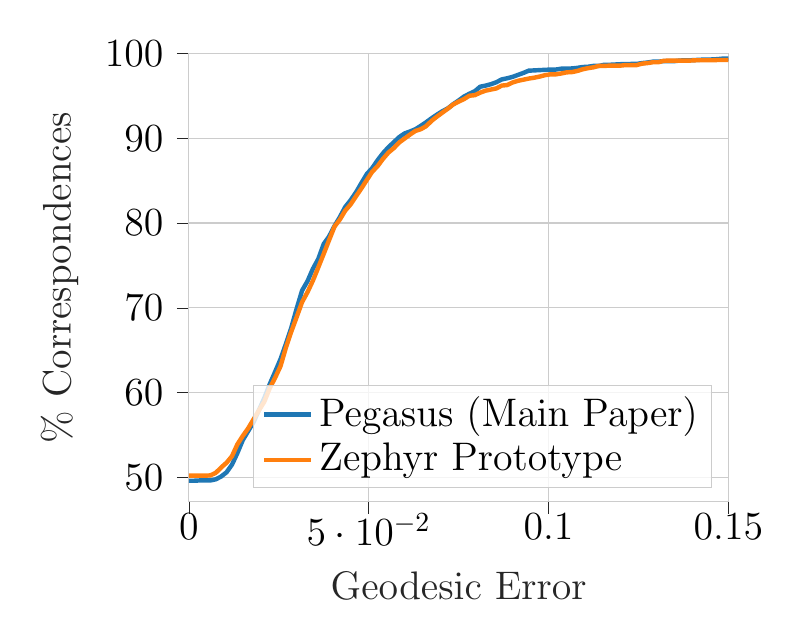
\begin{tikzpicture}

\definecolor{darkorange25512714}{RGB}{255,127,14}
\definecolor{darkslategray38}{RGB}{38,38,38}
\definecolor{lightgray204}{RGB}{204,204,204}
\definecolor{steelblue31119180}{RGB}{31,119,180}

\Large
\begin{axis}[
axis line style={lightgray204},
legend cell align={left},
legend style={
  fill opacity=0.8,
  draw opacity=1,
  text opacity=1,
  at={(0.97,0.03)},
  anchor=south east,
  draw=lightgray204
},
tick align=outside,
tick pos=left,
x grid style={lightgray204},
xlabel=\textcolor{darkslategray38}{Geodesic Error},
xmajorgrids,
xtick = {0,0.05,0.1,0.15},
xmin=0, xmax=0.15,
xtick style={color=darkslategray38},
xticklabel style={yshift= 5pt},
y grid style={lightgray204},
ylabel=\textcolor{darkslategray38}{\% Correspondences},
ymajorgrids,
ymin=47.1115537848606, ymax=100,
ytick style={color=darkslategray38}
]
\addplot [ultra thick, steelblue31119180]
table {%
0 49.601593625498
0.0015 49.601593625498
0.003 49.6347941567065
0.0045 49.6347941567065
0.006 49.6347941567065
0.0075 49.7675962815405
0.009 50.0996015936255
0.0105 50.597609561753
0.012 51.4940239043825
0.0135 52.8552456839309
0.015 54.3824701195219
0.0165 55.4448871181939
0.018 56.5073041168659
0.0195 57.9349269588313
0.021 59.3625498007968
0.0225 60.9893758300133
0.024 62.4501992031873
0.0255 63.9442231075697
0.027 65.7370517928287
0.0285 67.6626826029216
0.03 69.9203187250996
0.0315 72.0451527224436
0.033 73.140770252324
0.0345 74.601593625498
0.036 75.7636122177955
0.0375 77.5232403718459
0.039 78.4196547144754
0.0405 79.6480743691899
0.042 80.7104913678619
0.0435 81.9057104913679
0.045 82.7025232403718
0.0465 83.6321381142098
0.048 84.7277556440903
0.0495 85.7901726427623
0.051 86.4873837981408
0.0525 87.4169986719788
0.054 88.2470119521912
0.0555 88.9442231075697
0.057 89.5418326693227
0.0585 90.1394422310757
0.06 90.5710491367862
0.0615 90.8034528552457
0.063 91.0690571049137
0.0645 91.4674634794157
0.066 91.8990703851262
0.0675 92.3638778220452
0.069 92.7954847277556
0.0705 93.1938911022576
0.072 93.5258964143426
0.0735 94.0239043824701
0.075 94.4555112881806
0.0765 94.9203187250996
0.078 95.2523240371846
0.0795 95.5511288180611
0.081 96.0823373173971
0.0825 96.2151394422311
0.084 96.3811420982736
0.0855 96.6135458167331
0.087 96.9455511288181
0.0885 97.0783532536521
0.09 97.2443559096945
0.0915 97.4767596281541
0.093 97.7091633466136
0.0945 97.9747675962815
0.096 98.00796812749
0.0975 98.0411686586986
0.099 98.074369189907
0.1005 98.1075697211156
0.102 98.1075697211156
0.1035 98.207171314741
0.105 98.207171314741
0.1065 98.2403718459495
0.108 98.3067729083665
0.1095 98.406374501992
0.111 98.4395750332005
0.1125 98.539176626826
0.114 98.539176626826
0.1155 98.67197875166
0.117 98.67197875166
0.1185 98.7051792828685
0.12 98.738379814077
0.1215 98.738379814077
0.123 98.7715803452855
0.1245 98.7715803452855
0.126 98.871181938911
0.1275 98.937583001328
0.129 99.0371845949535
0.1305 99.0371845949535
0.132 99.1035856573705
0.1335 99.1035856573705
0.135 99.1035856573705
0.1365 99.1699867197875
0.138 99.203187250996
0.1395 99.203187250996
0.141 99.2363877822045
0.1425 99.269588313413
0.144 99.269588313413
0.1455 99.3027888446215
0.147 99.33598937583
0.1485 99.402390438247
0.15 99.402390438247
};
\addlegendentry{Pegasus (Main Paper)}
\addplot [ultra thick, darkorange25512714]
table {%
0 50.199203187251
0.0015 50.199203187251
0.003 50.199203187251
0.0045 50.199203187251
0.006 50.2324037184595
0.0075 50.531208499336
0.009 51.1620185922975
0.0105 51.726427622842
0.012 52.4900398406375
0.0135 53.8844621513944
0.015 54.8804780876494
0.0165 55.7768924302789
0.018 56.8393094289509
0.0195 57.9017264276228
0.021 58.9309428950863
0.0225 60.5245683930943
0.024 61.7529880478088
0.0255 63.1142098273572
0.027 65.3054448871182
0.0285 67.1978751660027
0.03 68.9243027888446
0.0315 70.6839309428951
0.033 71.8459495351926
0.0345 73.207171314741
0.036 74.7675962815405
0.0375 76.3612217795485
0.039 77.9880478087649
0.0405 79.5816733067729
0.042 80.4116865869854
0.0435 81.4741035856574
0.045 82.2045152722444
0.0465 83.1673306772908
0.048 84.0969455511288
0.0495 85.0929614873838
0.051 86.0557768924303
0.0525 86.7197875166003
0.054 87.5830013280212
0.0555 88.3134130146082
0.057 88.8446215139442
0.0585 89.5086321381142
0.06 89.9734395750332
0.0615 90.4382470119522
0.063 90.8698539176627
0.0645 91.0690571049137
0.066 91.4342629482072
0.0675 92.0650730411687
0.069 92.5630810092961
0.0705 93.0278884462151
0.072 93.4926958831341
0.0735 93.9907038512616
0.075 94.3227091633466
0.0765 94.6215139442231
0.078 95.0199203187251
0.0795 95.0863213811421
0.081 95.3851261620186
0.0825 95.6175298804781
0.084 95.7503320053121
0.0855 95.8831341301461
0.087 96.2151394422311
0.0885 96.2815405046481
0.09 96.5803452855246
0.0915 96.7795484727756
0.093 96.9123505976096
0.0945 97.0451527224436
0.096 97.1447543160691
0.0975 97.2775564409031
0.099 97.4435590969455
0.1005 97.543160690571
0.102 97.543160690571
0.1035 97.6427622841965
0.105 97.7755644090305
0.1065 97.808764940239
0.108 97.9415670650731
0.1095 98.140770252324
0.111 98.273572377158
0.1125 98.3731739707835
0.114 98.539176626826
0.1155 98.539176626826
0.117 98.5723771580345
0.1185 98.5723771580345
0.12 98.5723771580345
0.1215 98.6387782204515
0.123 98.6387782204515
0.1245 98.6387782204515
0.126 98.804780876494
0.1275 98.871181938911
0.129 98.9707835325365
0.1305 98.9707835325365
0.132 99.136786188579
0.1335 99.1699867197875
0.135 99.1699867197875
0.1365 99.1699867197875
0.138 99.1699867197875
0.1395 99.1699867197875
0.141 99.203187250996
0.1425 99.203187250996
0.144 99.203187250996
0.1455 99.203187250996
0.147 99.2363877822045
0.1485 99.2363877822045
0.15 99.2363877822045
};
\addlegendentry{Zephyr Prototype}
\end{axis}

\end{tikzpicture}
}
    \resizebox{0.48\linewidth}{!}{
    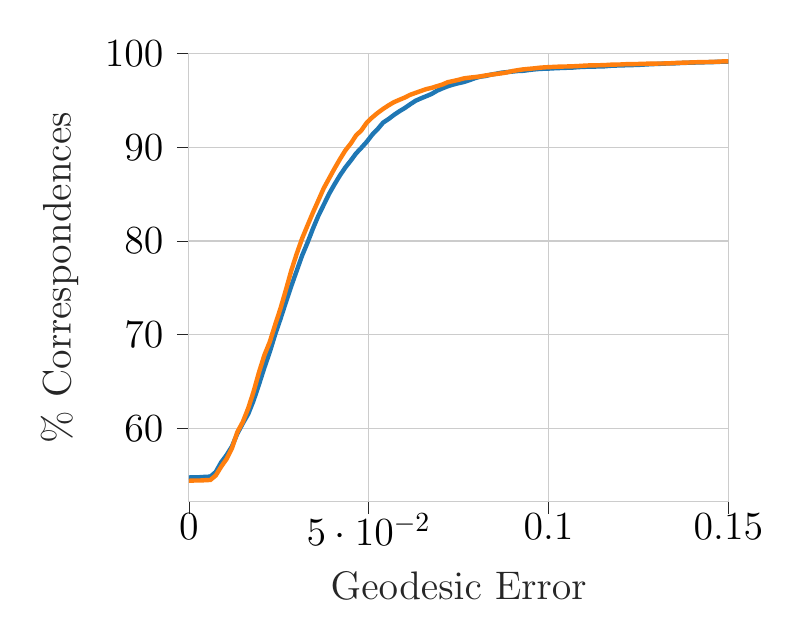
\begin{tikzpicture}

\definecolor{darkorange25512714}{RGB}{255,127,14}
\definecolor{darkslategray38}{RGB}{38,38,38}
\definecolor{forestgreen4416044}{RGB}{44,160,44}
\definecolor{lightgray204}{RGB}{204,204,204}
\definecolor{steelblue31119180}{RGB}{31,119,180}

\Large
\begin{axis}[
axis line style={lightgray204},
legend cell align={left},
legend style={
  fill opacity=0.8,
  draw opacity=1,
  text opacity=1,
  at={(0.97,0.03)},
  anchor=south east,
  draw=lightgray204
},
tick align=outside,
tick pos=left,
xtick = {0,0.05,0.1,0.15},
x grid style={lightgray204},
xlabel=\textcolor{darkslategray38}{Geodesic Error},
xmajorgrids,
xmin=0, xmax=0.15,
xtick style={color=darkslategray38},
xticklabel style={yshift= 5pt},
y grid style={lightgray204},
ylabel=\textcolor{darkslategray38}{\% Correspondences},
ymajorgrids,
ymin=52.1674413457282, ymax=100,
ytick style={color=darkslategray38}
]

\addplot [ultra thick, steelblue31119180]
table {%
0 54.763169544046
0.0015 54.7941567065073
0.003 54.7941567065073
0.0045 54.8317839752102
0.006 54.8605577689243
0.0075 55.3497122620629
0.009 56.3789287295263
0.0105 57.153607791058
0.012 58.0787959274015
0.0135 59.4510845506861
0.015 60.522355024347
0.0165 61.5316511730855
0.018 62.9681274900398
0.0195 64.6790615316512
0.021 66.4763169544046
0.0225 68.1474103585657
0.024 70.0177069499778
0.0255 71.7020805666224
0.027 73.481629039398
0.0285 75.1947764497565
0.03 76.8260292164674
0.0315 78.444001770695
0.033 79.8162903939796
0.0345 81.3036741921204
0.036 82.6715360779106
0.0375 83.8490482514387
0.039 85.0265604249668
0.0405 86.0358565737052
0.042 86.9853917662683
0.0435 87.8331119964586
0.045 88.5613103142984
0.0465 89.3426294820717
0.048 89.9513058875609
0.0495 90.5953961930057
0.051 91.3457281983178
0.0525 91.9344842850819
0.054 92.6228419654714
0.0555 93.0035413899956
0.057 93.4373616644533
0.0585 93.8291279327136
0.06 94.1722000885348
0.0615 94.572819831784
0.063 94.9513058875609
0.0645 95.2102700309872
0.066 95.4448871181939
0.0675 95.6883576803895
0.069 96.0292164674634
0.0705 96.281540504648
0.072 96.5073041168658
0.0735 96.6888003541389
0.075 96.8348826914563
0.0765 96.9654714475431
0.078 97.1536077910579
0.0795 97.3660911907924
0.081 97.5276671093404
0.0825 97.6029216467463
0.084 97.7467906153165
0.0855 97.846392208942
0.087 97.9570606463037
0.0885 98.0168216024789
0.09 98.074369189907
0.0915 98.1363435148295
0.093 98.1584772023019
0.0945 98.235945108455
0.096 98.3045595396193
0.0975 98.3554670208056
0.099 98.3820274457724
0.1005 98.3997343957503
0.102 98.435148295706
0.1035 98.4550686144311
0.105 98.4772023019035
0.1065 98.4904825143869
0.108 98.5413899955732
0.1095 98.5723771580345
0.111 98.5945108455068
0.1125 98.6033643204958
0.114 98.6188579017264
0.1155 98.6321381142098
0.117 98.6852589641434
0.1185 98.7118193891101
0.12 98.729526339088
0.1215 98.7472332890659
0.123 98.7649402390438
0.1245 98.7782204515272
0.126 98.8069942452412
0.1275 98.8424081451969
0.129 98.8733953076582
0.1305 98.8888888888889
0.132 98.9243027888446
0.1335 98.9397963700752
0.135 98.9508632138114
0.1365 98.9840637450199
0.138 99.0061974324922
0.1395 99.0239043824701
0.141 99.0393979637007
0.1425 99.0593182824258
0.144 99.0681717574147
0.1455 99.0836653386454
0.147 99.1146525011067
0.1485 99.1212926073484
0.15 99.1212926073484
};
\addplot [ultra thick, darkorange25512714]
table {%
0 54.4134572819831
0.0015 54.4422310756972
0.003 54.4422310756972
0.0045 54.4732182381585
0.006 54.5042054006197
0.0075 54.9822930500221
0.009 55.920761398849
0.0105 56.7352810978309
0.012 57.8795927401505
0.0135 59.6082337317397
0.015 60.6795042054006
0.0165 62.1292607348384
0.018 63.9065958388668
0.0195 65.9650287737937
0.021 67.7999114652501
0.0225 69.2164674634794
0.024 71.0469234174414
0.0255 72.8087649402391
0.027 74.7853032315184
0.0285 76.850376272687
0.03 78.6321381142099
0.0315 80.2633908809208
0.033 81.651173085436
0.0345 83.0190349712262
0.036 84.3116423196105
0.0375 85.6153165117309
0.039 86.6733067729084
0.0405 87.722443559097
0.042 88.7162461266047
0.0435 89.6525011066844
0.045 90.3829127932713
0.0465 91.2549800796812
0.048 91.8149623727313
0.0495 92.6383355467021
0.051 93.1850376272687
0.0525 93.6631252766711
0.054 94.0858787073927
0.0555 94.4643647631695
0.057 94.8030101814962
0.0585 95.0553342186808
0.06 95.2943780433821
0.0615 95.588756086764
0.063 95.796812749004
0.0645 96.0004426737494
0.066 96.2018592297476
0.0675 96.3346613545816
0.069 96.5161575918548
0.0705 96.6910137228862
0.072 96.9411243913236
0.0735 97.0628596724214
0.075 97.1956617972554
0.0765 97.3505976095618
0.078 97.4236387782204
0.0795 97.485613103143
0.081 97.5586542718016
0.0825 97.6626826029216
0.084 97.7379371403276
0.0855 97.817618415228
0.087 97.8906595838866
0.0885 97.9902611775121
0.09 98.1319167773351
0.0915 98.2270916334661
0.093 98.3089862771137
0.0945 98.3643204957945
0.096 98.4152279769809
0.0975 98.4838424081452
0.099 98.5281097830898
0.1005 98.5524568393094
0.102 98.5834440017706
0.1035 98.605577689243
0.105 98.6166445329791
0.1065 98.6321381142097
0.108 98.6586985391765
0.1095 98.6963258078795
0.111 98.7250996015935
0.1125 98.7339530765825
0.114 98.7494466578131
0.1155 98.758300132802
0.117 98.8025675077466
0.1185 98.8202744577246
0.12 98.8313413014607
0.1215 98.8601150951748
0.123 98.8667552014165
0.1245 98.8822487826471
0.126 98.891102257636
0.1275 98.9176626826029
0.129 98.9265161575918
0.1305 98.9309428950862
0.132 98.937583001328
0.1335 98.9530765825586
0.135 98.9884904825143
0.1365 99.0084108012394
0.138 99.0305444887117
0.1395 99.0460380699424
0.141 99.0703851261619
0.1425 99.0792386011509
0.144 99.0947321823815
0.1455 99.1035856573704
0.147 99.1257193448428
0.1485 99.1589198760513
0.15 99.1589198760513
};

\end{axis}

\end{tikzpicture}
} 
    \caption{ 
    PCK curves for (left) a three-shape and (right) a ten-shape inter-class FAUST instance on both QPU architectures. %
    } 
    \label{fig:InterClassQPU} 
\end{figure} 

\begin{figure}
    \centering
    \resizebox{0.49\linewidth}{!}{
    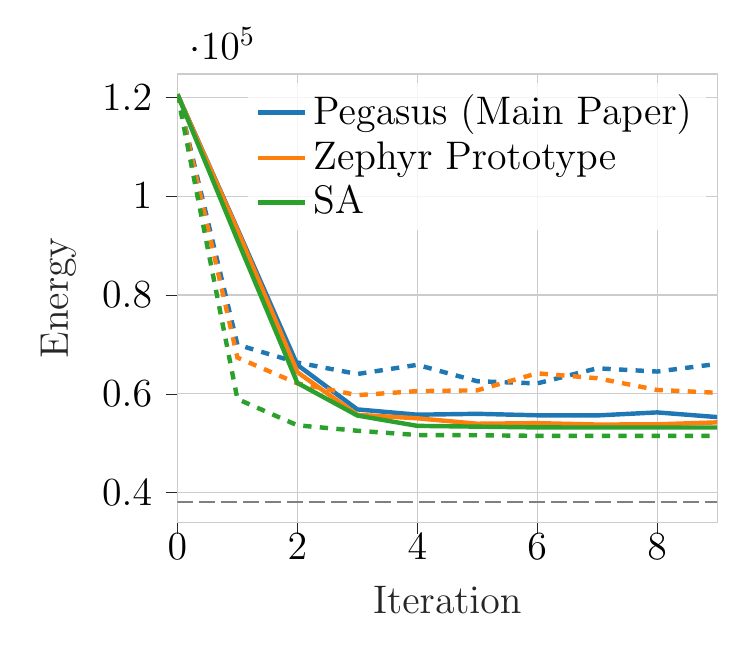
\begin{tikzpicture}

\definecolor{darkorange25512714}{RGB}{255,127,14}
\definecolor{darkslategray38}{RGB}{38,38,38}
\definecolor{forestgreen4416044}{RGB}{44,160,44}
\definecolor{gray}{RGB}{128,128,128}
\definecolor{lightgray204}{RGB}{204,204,204}
\definecolor{steelblue31119180}{RGB}{31,119,180}

\Large
\begin{axis}[
axis line style={lightgray204},
legend cell align={left},
legend style={fill opacity=0.8, draw opacity=1, text opacity=1, draw=none},
tick align=outside,
tick pos=left,
x grid style={lightgray204},
xlabel=\textcolor{darkslategray38}{Iteration},
xmajorgrids,
xmin=0, xmax=9,
xtick style={color=darkslategray38},
xticklabel style={yshift= 5pt},
y grid style={lightgray204},
ylabel=\textcolor{darkslategray38}{Energy},
ymajorgrids,
ymin=34035.05, ymax=124695.95,
ytick style={color=darkslategray38}
]

\addplot [ultra thick, steelblue31119180]
table {%
0 120575
1 93379.7859163443
2 65856.5540745175
3 56859.9989051177
4 55788.5351135226
5 55966.5265769375
6 55667.9724943428
7 55642.2407912453
8 56251.7817966032
9 55310.1550710056
};
\addlegendentry{Pegasus (Main Paper)}
\addplot [ultra thick, steelblue31119180, dashed, forget plot]
table {%
0 120575
1 69943.4553888252
2 66342.7915206047
3 64016.3755693446
4 65876.1730058255
5 62550.7472240753
6 62120.6832089319
7 65168.2282910738
8 64517.2823635984
9 66055.0810633431
};
\addplot [ultra thick, darkorange25512714]
table {%
0 120575
1 93138.6592221228
2 64395.8443103471
3 55764.3192470843
4 55063.0161003932
5 53960.8348714902
6 54082.2253346483
7 53797.6614173209
8 53843.8312559086
9 54235.8511564518
};
\addlegendentry{Zephyr Prototype}
\addplot [ultra thick, darkorange25512714, dashed, forget plot]
table {%
0 120575
1 67345.7011906687
2 62116.4510778603
3 59744.6481853321
4 60555.3274782254
5 60718.3256542676
6 64160.1567897874
7 63162.0652870842
8 60797.5553337758
9 60221.6952612643
};
\path [draw=gray, semithick, dash pattern=on 5.55pt off 2.4pt]
(axis cs:0,38156)
--(axis cs:10,38156);

\addplot [ultra thick, forestgreen4416044]
table {%
0 120575
1 91142.904325786
2 62211.7790507435
3 55623.5223354449
4 53529.4107996722
5 53374.1822750181
6 53214.7761427653
7 53197.9737940531
8 53197.9737940531
9 53197.9737940531
};
\addlegendentry{SA}
\addplot [ultra thick, forestgreen4416044, dashed, forget plot]
table {%
0 120575
1 58960.4301751069
2 53646.1820547435
3 52543.3119711551
4 51678.8554060219
5 51631.1356493409
6 51515.6549776222
7 51515.6549776222
8 51515.6549776222
9 51515.6549776222
};

\end{axis}

\end{tikzpicture}
}
    \resizebox{0.49\linewidth}{!}{
    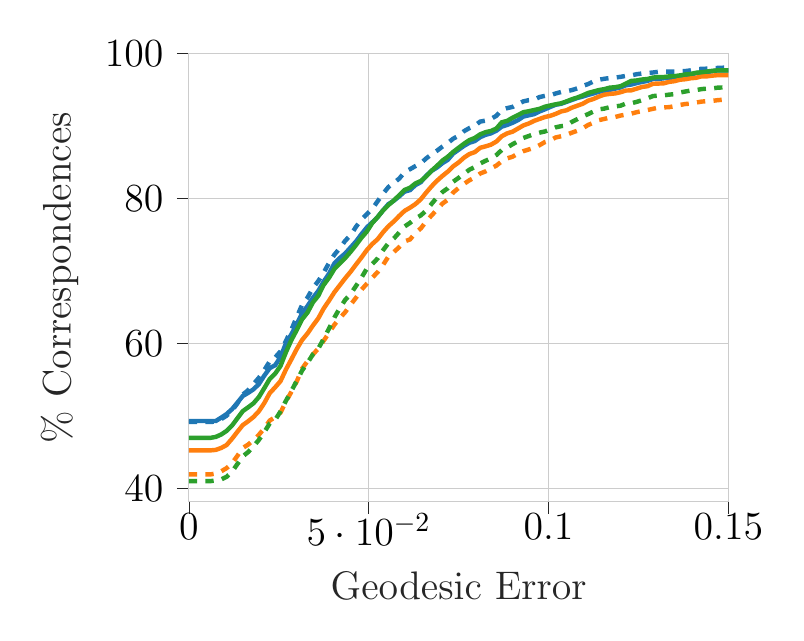
\begin{tikzpicture}

\definecolor{darkorange25512714}{RGB}{255,127,14}
\definecolor{darkslategray38}{RGB}{38,38,38}
\definecolor{forestgreen4416044}{RGB}{44,160,44}
\definecolor{lightgray204}{RGB}{204,204,204}
\definecolor{steelblue31119180}{RGB}{31,119,180}

\Large
\begin{axis}[
axis line style={lightgray204},
legend cell align={left},
legend style={
  fill opacity=0.8,
  draw opacity=1,
  text opacity=1,
  at={(0.65,0.15)},
  anchor=center,
  draw=lightgray204
},
tick align=outside,
tick pos=left,
xtick = {0,0.05,0.1,0.15},
x grid style={lightgray204},
xlabel=\textcolor{darkslategray38}{Geodesic Error},
xmajorgrids,
xmin=0, xmax=0.15,
xtick style={color=darkslategray38},
xticklabel style={yshift= 5pt},
y grid style={lightgray204},
ylabel=\textcolor{darkslategray38}{\% Correspondences},
ymajorgrids,
ymin=38.1158698539177, ymax=100,
ytick style={color=darkslategray38}
]
\addplot [ultra thick, steelblue31119180]
table {%
0 49.269588313413
0.0015 49.269588313413
0.003 49.269588313413
0.0045 49.269588313413
0.006 49.269588313413
0.0075 49.269588313413
0.009 49.734395750332
0.0105 50.2324037184595
0.012 50.8964143426295
0.0135 51.792828685259
0.015 52.7224435590969
0.0165 53.1540504648074
0.018 53.6520584329349
0.0195 54.3824701195219
0.021 55.5444887118194
0.0225 56.5737051792829
0.024 56.9721115537849
0.0255 58.1009296148738
0.027 59.9933598937583
0.0285 61.2217795484728
0.03 62.6162018592298
0.0315 64.1434262948207
0.033 65.1394422310757
0.0345 66.2682602921647
0.036 67.2310756972112
0.0375 68.5258964143426
0.039 69.6215139442231
0.0405 71.0491367861886
0.042 71.7795484727756
0.0435 72.410358565737
0.045 73.2403718459495
0.0465 74.070385126162
0.048 75.066401062417
0.0495 75.996015936255
0.051 76.6932270916335
0.0525 77.4236387782205
0.054 78.3532536520584
0.0555 79.2164674634794
0.057 79.6812749003984
0.0585 80.2788844621514
0.06 80.9428950863214
0.0615 81.1420982735724
0.063 81.8393094289509
0.0645 82.2377158034528
0.066 83.1341301460823
0.0675 83.7981407702523
0.069 84.2629482071713
0.0705 84.8605577689243
0.072 85.3253652058433
0.0735 86.1885790172643
0.075 86.7197875166003
0.0765 87.2509960159363
0.078 87.6826029216467
0.0795 87.9150066401063
0.081 88.4462151394422
0.0825 88.7782204515272
0.084 88.9774236387782
0.0855 89.3426294820717
0.087 89.9070385126162
0.0885 90.1394422310757
0.09 90.4382470119522
0.0915 90.8034528552457
0.093 91.3014608233732
0.0945 91.4674634794157
0.096 91.6334661354582
0.0975 91.9986719787517
0.099 92.2974767596282
0.1005 92.6294820717132
0.102 92.9282868525896
0.1035 93.0610889774236
0.105 93.3266932270916
0.1065 93.5922974767596
0.108 93.8579017264276
0.1095 94.0571049136786
0.111 94.2895086321381
0.1125 94.4887118193891
0.114 94.7211155378486
0.1155 94.8539176626826
0.117 94.9867197875166
0.1185 95.1527224435591
0.12 95.3187250996016
0.1215 95.6175298804781
0.123 95.7171314741036
0.1245 95.9163346613546
0.126 96.0823373173971
0.1275 96.2151394422311
0.129 96.4807436918991
0.1305 96.4807436918991
0.132 96.5803452855246
0.1335 96.6135458167331
0.135 96.6135458167331
0.1365 96.8459495351926
0.138 96.9455511288181
0.1395 97.1115537848606
0.141 97.2775564409031
0.1425 97.4103585657371
0.144 97.4435590969455
0.1455 97.543160690571
0.147 97.675962815405
0.1485 97.675962815405
0.15 97.675962815405
};
\addplot [ultra thick, steelblue31119180, dashed, forget plot]
table {%
0 49.136786188579
0.0015 49.136786188579
0.003 49.136786188579
0.0045 49.136786188579
0.006 49.136786188579
0.0075 49.203187250996
0.009 49.535192563081
0.0105 50
0.012 50.6972111553785
0.0135 51.6932270916335
0.015 52.9216467463479
0.0165 53.5192563081009
0.018 54.3824701195219
0.0195 55.2456839309429
0.021 56.3081009296149
0.0225 57.5033200531209
0.024 58.0345285524568
0.0255 58.8977423638778
0.027 60.3253652058433
0.0285 61.8525896414343
0.03 63.6122177954847
0.0315 65.3054448871182
0.033 66.3014608233732
0.0345 67.6294820717132
0.036 68.5922974767596
0.0375 69.7543160690571
0.039 71.1155378486056
0.0405 72.2443559096946
0.042 73.140770252324
0.0435 74.1699867197875
0.045 74.933598937583
0.0465 76.0956175298805
0.048 77.0916334661355
0.0495 77.8220451527224
0.051 78.5524568393094
0.0525 79.6148738379814
0.054 80.6440903054449
0.0555 81.5737051792829
0.057 82.1381142098274
0.0585 82.7357237715804
0.06 83.6321381142098
0.0615 84.0305444887118
0.063 84.4621513944223
0.0645 84.8605577689243
0.066 85.5245683930943
0.0675 86.0889774236388
0.069 86.5869853917663
0.0705 87.1513944223108
0.072 87.6494023904383
0.0735 88.2470119521912
0.075 88.6454183266932
0.0765 89.2762284196547
0.078 89.7078353253652
0.0795 90.0398406374502
0.081 90.6042496679947
0.0825 90.7370517928287
0.084 90.9694555112882
0.0855 91.4010624169987
0.087 92.2310756972112
0.0885 92.4634794156706
0.09 92.6294820717132
0.0915 93.0278884462152
0.093 93.3930942895086
0.0945 93.5590969455511
0.096 93.6254980079681
0.0975 93.9907038512616
0.099 94.1567065073041
0.1005 94.2231075697211
0.102 94.4887118193891
0.1035 94.6879150066401
0.105 94.7875166002656
0.1065 94.9535192563081
0.108 95.1859229747676
0.1095 95.5179282868526
0.111 95.7835325365206
0.1125 96.1487383798141
0.114 96.3811420982736
0.1155 96.5139442231076
0.117 96.6135458167331
0.1185 96.6799468791501
0.12 96.7795484727756
0.1215 96.9123505976096
0.123 96.9787516600266
0.1245 97.1447543160691
0.126 97.2443559096945
0.1275 97.3107569721115
0.129 97.3771580345285
0.1305 97.476759628154
0.132 97.476759628154
0.1335 97.5099601593625
0.135 97.5099601593625
0.1365 97.543160690571
0.138 97.5763612217796
0.1395 97.6759628154051
0.141 97.8419654714476
0.1425 97.875166002656
0.144 97.9083665338645
0.1455 97.9747675962815
0.147 98.00796812749
0.1485 98.0411686586985
0.15 98.0411686586985
};
\addplot [ultra thick, darkorange25512714]
table {%
0 45.2191235059761
0.0015 45.2191235059761
0.003 45.2191235059761
0.0045 45.2191235059761
0.006 45.2191235059761
0.0075 45.2855245683931
0.009 45.5511288180611
0.0105 45.9495351925631
0.012 46.8127490039841
0.0135 47.7755644090305
0.015 48.7051792828685
0.0165 49.2363877822045
0.018 49.8339973439575
0.0195 50.6308100929615
0.021 51.7596281540505
0.0225 53.1208499335989
0.024 53.9176626826029
0.0255 54.7808764940239
0.027 56.3745019920319
0.0285 57.7689243027889
0.03 59.1965471447543
0.0315 60.4581673306773
0.033 61.3545816733068
0.0345 62.4501992031872
0.036 63.4462151394422
0.0375 64.8074369189907
0.039 65.9030544488712
0.0405 67.0650730411687
0.042 68.0278884462151
0.0435 68.9907038512616
0.045 69.8871181938911
0.0465 70.8831341301461
0.048 71.8459495351926
0.0495 72.875166002656
0.051 73.7051792828685
0.0525 74.3691899070385
0.054 75.332005312085
0.0555 76.1620185922975
0.057 76.8260292164675
0.0585 77.5896414342629
0.06 78.2868525896414
0.0615 78.7184594953519
0.063 79.2164674634794
0.0645 79.8804780876494
0.066 80.8100929614874
0.0675 81.6733067729084
0.069 82.4369189907038
0.0705 83.1009296148738
0.072 83.6985391766268
0.0735 84.4289508632138
0.075 84.9601593625498
0.0765 85.6241699867198
0.078 86.1221779548473
0.0795 86.3877822045153
0.081 86.9853917662683
0.0825 87.1845949535193
0.084 87.4169986719788
0.0855 87.8486055776892
0.087 88.5790172642762
0.0885 88.9774236387782
0.09 89.2098273572377
0.0915 89.6414342629482
0.093 90.0730411686587
0.0945 90.3386454183267
0.096 90.7038512616202
0.0975 90.9694555112882
0.099 91.2350597609562
0.1005 91.4010624169987
0.102 91.6666666666667
0.1035 91.9986719787517
0.105 92.1646746347942
0.1065 92.5298804780876
0.108 92.7954847277556
0.1095 93.0610889774236
0.111 93.4926958831341
0.1125 93.7250996015936
0.114 94.0571049136786
0.1155 94.3227091633466
0.117 94.4223107569721
0.1185 94.4887118193891
0.12 94.6547144754316
0.1215 94.8871181938911
0.123 94.9203187250996
0.1245 95.1527224435591
0.126 95.3851261620186
0.1275 95.4847277556441
0.129 95.8167330677291
0.1305 95.8499335989376
0.132 95.8831341301461
0.1335 96.0823373173971
0.135 96.1819389110226
0.1365 96.3811420982736
0.138 96.4475431606906
0.1395 96.5803452855246
0.141 96.6467463479416
0.1425 96.8459495351926
0.144 96.8459495351926
0.1455 96.9455511288181
0.147 97.011952191235
0.1485 97.011952191235
0.15 97.011952191235
};
\addplot [ultra thick, darkorange25512714, dashed, forget plot]
table {%
0 41.8990703851262
0.0015 41.8990703851262
0.003 41.8990703851262
0.0045 41.8990703851262
0.006 41.8990703851262
0.0075 42.0318725099602
0.009 42.3306772908367
0.0105 42.7622841965471
0.012 43.4262948207171
0.0135 44.4555112881806
0.015 45.5511288180611
0.0165 46.0159362549801
0.018 46.6467463479416
0.0195 47.3771580345286
0.021 48.273572377158
0.0225 49.33598937583
0.024 49.800796812749
0.0255 50.4316069057105
0.027 51.9588313413015
0.0285 53.2868525896414
0.03 54.7144754316069
0.0315 56.5073041168659
0.033 57.5365205843293
0.0345 58.4661354581673
0.036 59.2629482071713
0.0375 60.3585657370518
0.039 61.4541832669323
0.0405 62.5830013280213
0.042 63.4794156706507
0.0435 64.3094289508632
0.045 65.3386454183267
0.0465 66.3014608233732
0.048 67.3970783532537
0.0495 68.2270916334661
0.051 69.0571049136786
0.0525 69.8207171314741
0.054 70.8167330677291
0.0555 71.9787516600266
0.057 72.609561752988
0.0585 73.273572377158
0.06 74.070385126162
0.0615 74.33598937583
0.063 75.2324037184595
0.0645 75.863213811421
0.066 76.8260292164675
0.0675 77.6560424966799
0.069 78.4528552456839
0.0705 79.2828685258964
0.072 79.8140770252324
0.0735 80.8100929614874
0.075 81.4409030544489
0.0765 82.0053120849934
0.078 82.5033200531209
0.0795 82.9017264276228
0.081 83.4329349269588
0.0825 83.7317397078353
0.084 84.1301460823373
0.0855 84.5285524568393
0.087 85.1261620185923
0.0885 85.5245683930943
0.09 85.7569721115538
0.0915 86.1885790172643
0.093 86.5205843293493
0.0945 86.7529880478088
0.096 86.9853917662683
0.0975 87.3505976095617
0.099 87.7822045152722
0.1005 88.0146082337317
0.102 88.4130146082337
0.1035 88.5790172642762
0.105 88.7782204515272
0.1065 89.0770252324037
0.108 89.3426294820717
0.1095 89.6746347941567
0.111 90.1394422310757
0.1125 90.4382470119522
0.114 90.8034528552457
0.1155 90.9694555112882
0.117 91.1686586985392
0.1185 91.2350597609562
0.12 91.4342629482072
0.1215 91.5670650730412
0.123 91.6998671978752
0.1245 91.8990703851262
0.126 92.0650730411687
0.1275 92.1978751660027
0.129 92.3638778220452
0.1305 92.5298804780876
0.132 92.5630810092961
0.1335 92.5962815405046
0.135 92.7290836653386
0.1365 92.8950863213811
0.138 93.0278884462151
0.1395 93.0942895086321
0.141 93.2270916334661
0.1425 93.3598937583001
0.144 93.4262948207171
0.1455 93.4594953519256
0.147 93.5590969455511
0.1485 93.6254980079681
0.15 93.6254980079681
};
\addplot [ultra thick, forestgreen4416044]
table {%
0 46.9455511288181
0.0015 46.9455511288181
0.003 46.9455511288181
0.0045 46.9455511288181
0.006 46.9455511288181
0.0075 47.0783532536521
0.009 47.4103585657371
0.0105 47.9083665338645
0.012 48.6387782204515
0.0135 49.6347941567065
0.015 50.6308100929615
0.0165 51.1620185922975
0.018 51.726427622842
0.0195 52.589641434263
0.021 53.8180610889774
0.0225 55.0796812749004
0.024 55.8100929614874
0.0255 56.8725099601594
0.027 58.7649402390438
0.0285 60.4249667994688
0.03 61.8193891102258
0.0315 63.3134130146082
0.033 64.2430278884462
0.0345 65.6374501992032
0.036 66.5670650730412
0.0375 68.0610889774237
0.039 69.0571049136786
0.0405 70.2855245683931
0.042 71.0159362549801
0.0435 71.7795484727756
0.045 72.6427622841966
0.0465 73.5723771580345
0.048 74.5683930942895
0.0495 75.4316069057105
0.051 76.593625498008
0.0525 77.4236387782205
0.054 78.3532536520584
0.0555 79.0836653386454
0.057 79.7144754316069
0.0585 80.4448871181939
0.06 81.1752988047809
0.0615 81.4741035856574
0.063 82.0717131474104
0.0645 82.4037184594954
0.066 83.0345285524568
0.0675 83.8313413014608
0.069 84.4953519256308
0.0705 85.2257636122178
0.072 85.7569721115538
0.0735 86.4209827357238
0.075 86.9853917662683
0.0765 87.5498007968127
0.078 88.0478087649402
0.0795 88.3466135458167
0.081 88.8446215139442
0.0825 89.1434262948207
0.084 89.3094289508632
0.0855 89.6414342629482
0.087 90.5046480743692
0.0885 90.7038512616202
0.09 91.1354581673307
0.0915 91.5006640106242
0.093 91.8990703851262
0.0945 92.0318725099601
0.096 92.1978751660026
0.0975 92.3638778220452
0.099 92.6626826029216
0.1005 92.8286852589641
0.102 92.9946879150066
0.1035 93.1274900398407
0.105 93.3930942895086
0.1065 93.6918990703851
0.108 93.9243027888446
0.1095 94.2231075697211
0.111 94.5551128818061
0.1125 94.7543160690571
0.114 94.9535192563081
0.1155 95.0863213811421
0.117 95.2855245683931
0.1185 95.3519256308101
0.12 95.4847277556441
0.1215 95.8499335989376
0.123 96.2151394422311
0.1245 96.2815405046481
0.126 96.4143426294821
0.1275 96.4807436918991
0.129 96.6799468791501
0.1305 96.7463479415671
0.132 96.7463479415671
0.1335 96.8459495351926
0.135 96.8791500664011
0.1365 96.9787516600266
0.138 97.1115537848606
0.1395 97.1779548472775
0.141 97.3439575033201
0.1425 97.4103585657371
0.144 97.5099601593625
0.1455 97.609561752988
0.147 97.675962815405
0.1485 97.675962815405
0.15 97.675962815405
};
\addplot [ultra thick, forestgreen4416044, dashed, forget plot]
table {%
0 40.9694555112882
0.0015 40.9694555112882
0.003 40.9694555112882
0.0045 40.9694555112882
0.006 40.9694555112882
0.0075 41.0690571049137
0.009 41.2018592297477
0.0105 41.5670650730412
0.012 42.2642762284197
0.0135 43.3266932270916
0.015 44.3891102257636
0.0165 44.9867197875166
0.018 45.7835325365206
0.0195 46.6799468791501
0.021 47.742363877822
0.0225 48.937583001328
0.024 49.402390438247
0.0255 50.597609561753
0.027 52.058432934927
0.0285 53.3864541832669
0.03 54.8140770252324
0.0315 56.2416998671979
0.033 57.3041168658698
0.0345 58.4661354581673
0.036 59.2629482071713
0.0375 60.6241699867198
0.039 62.0517928286853
0.0405 63.5790172642762
0.042 64.8738379814077
0.0435 66.0026560424967
0.045 66.8326693227092
0.0465 67.9282868525896
0.048 69.0571049136786
0.0495 70.3187250996016
0.051 70.9495351925631
0.0525 71.7131474103586
0.054 72.8419654714476
0.0555 73.8379814077025
0.057 74.468791500664
0.0585 75.2988047808765
0.06 76.128818061089
0.0615 76.6268260292165
0.063 77.2244355909695
0.0645 77.6560424966799
0.066 78.3200531208499
0.0675 79.2496679946879
0.069 80.1460823373174
0.0705 80.8764940239044
0.072 81.4077025232404
0.0735 82.3041168658699
0.075 82.8353253652058
0.0765 83.3997343957503
0.078 83.9641434262948
0.0795 84.3293492695883
0.081 84.8273572377158
0.0825 85.1925630810093
0.084 85.5245683930943
0.0855 85.9893758300133
0.087 86.6865869853918
0.0885 87.0185922974768
0.09 87.4833997343957
0.0915 87.8818061088977
0.093 88.3466135458167
0.0945 88.6122177954847
0.096 88.8778220451527
0.0975 89.0770252324037
0.099 89.2430278884462
0.1005 89.5086321381142
0.102 89.8074369189907
0.1035 89.9734395750332
0.105 90.0730411686587
0.1065 90.5710491367862
0.108 90.9362549800797
0.1095 91.3346613545817
0.111 91.6334661354582
0.1125 91.9986719787517
0.114 92.2974767596281
0.1155 92.3970783532536
0.117 92.5962815405047
0.1185 92.6958831341302
0.12 92.7954847277556
0.1215 93.0942895086321
0.123 93.1274900398406
0.1245 93.3266932270916
0.126 93.5590969455511
0.1275 93.8247011952191
0.129 94.1235059760956
0.1305 94.1899070385126
0.132 94.2231075697211
0.1335 94.3227091633466
0.135 94.3891102257636
0.1365 94.6215139442231
0.138 94.7543160690571
0.1395 94.8871181938911
0.141 94.9535192563081
0.1425 95.0863213811421
0.144 95.1527224435591
0.1455 95.1859229747676
0.147 95.2855245683931
0.1485 95.3187250996016
0.15 95.3187250996016
};
\end{axis}

\end{tikzpicture}
}
    \caption{Quantitative results when using (solid) 20 and (dashed) 40 worst vertices on a three-shape FAUST instance. 
    We show (left) the energy evolution during optimisation and (right) the final PCK curves. 
    }
    \label{fig:Energy40}
\end{figure}

\begin{figure}[th]
    \centering
    \resizebox{0.48\linewidth}{!}{
    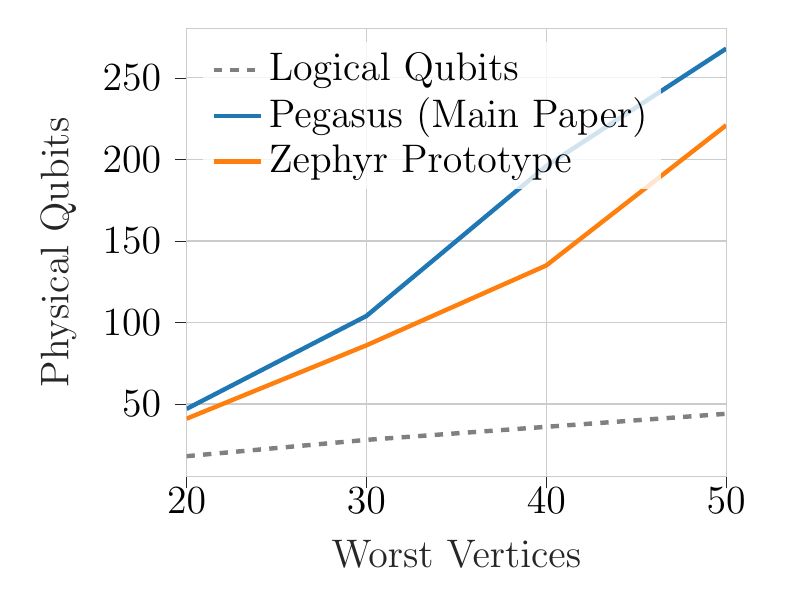
\begin{tikzpicture}

\definecolor{darkorange25512714}{RGB}{255,127,14}
\definecolor{darkslategray38}{RGB}{38,38,38}
\definecolor{gray}{RGB}{128,128,128}
\definecolor{lightgray204}{RGB}{204,204,204}
\definecolor{steelblue31119180}{RGB}{31,119,180}

\Large
\begin{axis}[
axis line style={lightgray204},
legend cell align={left},
legend style={
  fill opacity=0.8,
  draw opacity=1,
  text opacity=1,
  at={(0.03,0.97)},
  anchor=north west,
  draw=none
},
tick align=outside,
tick pos=left,
xtick = {20,30,40,50},
x grid style={lightgray204},
xmajorgrids,
xmin=20, xmax=50,
xtick style={color=darkslategray38},
xlabel=\textcolor{darkslategray38}{Worst Vertices},
xticklabel style={yshift= 5pt},
y grid style={lightgray204},
ymajorgrids,
ymin=5.5, ymax=280.5,
ytick style={color=darkslategray38},
ylabel=\textcolor{darkslategray38}{Physical Qubits},
]
\addplot [ultra thick, gray, dashed]
table {%
20 18
30 28
40 36
50 44
};
\addlegendentry{Logical Qubits}
\addplot [ultra thick, steelblue31119180]
table {%
20 47
30 104
40 196
50 268
};
\addlegendentry{Pegasus (Main Paper)}
\addplot [ultra thick, darkorange25512714]
table {%
20 41
30 86
40 135
50 221
};
\addlegendentry{Zephyr Prototype}
\end{axis}

\end{tikzpicture}
}
    \resizebox{0.48\linewidth}{!}{
    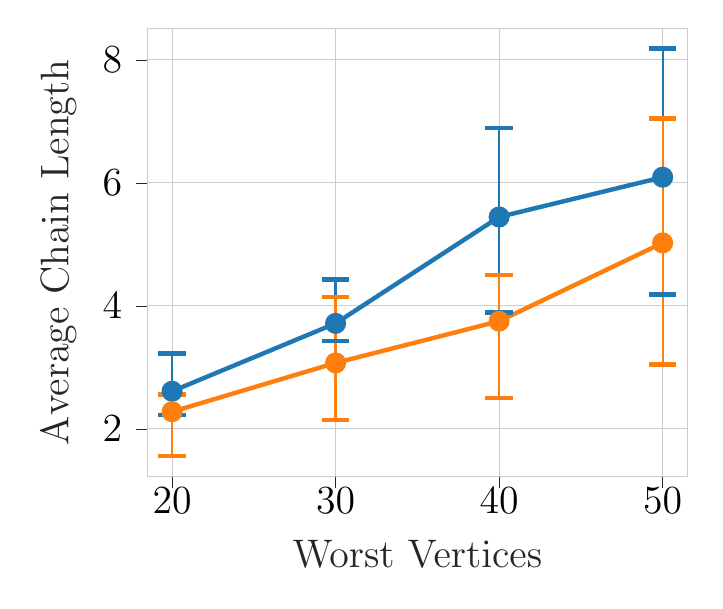
\begin{tikzpicture}

\definecolor{darkorange25512714}{RGB}{255,127,14}
\definecolor{darkslategray38}{RGB}{38,38,38}
\definecolor{lightgray204}{RGB}{204,204,204}
\definecolor{steelblue31119180}{RGB}{31,119,180}

\Large
\begin{axis}[
axis line style={lightgray204},
legend cell align={left},
legend style={
  fill opacity=0.8,
  draw opacity=1,
  text opacity=1,
  at={(0.03,0.97)},
  anchor=north west,
  draw=none
},
tick align=outside,
tick pos=left,
xtick = {20,30,40,50},
x grid style={lightgray204},
xmajorgrids,
xmin=18.5, xmax=51.5,
xtick style={color=darkslategray38},
xticklabel style={yshift= 5pt},
xlabel=\textcolor{darkslategray38}{Worst Vertices},
y grid style={lightgray204},
ymajorgrids,
ymin=1.22424242424242, ymax=8.51313131313131,
ytick style={color=darkslategray38},
ylabel=\textcolor{darkslategray38}{Average Chain Length},
]



\addplot [ultra thick, darkorange25512714, mark=-, mark size=5, mark options={solid}, only marks]
table {%
20 1.55555555555556
30 2.14285714285714
40 2.5
50 3.04545454545454
};


\path [draw=steelblue31119180, thick]
(axis cs:20,2.22222222222222)
--(axis cs:20,3.22222222222222);

\path [draw=steelblue31119180, thick]
(axis cs:30,3.42857142857143)
--(axis cs:30,4.42857142857143);

\path [draw=steelblue31119180, thick]
(axis cs:40,3.88888888888889)
--(axis cs:40,6.88888888888889);

\path [draw=steelblue31119180, thick]
(axis cs:50,4.18181818181818)
--(axis cs:50,8.18181818181818);

\addplot [ultra thick, steelblue31119180, mark=-, mark size=5, mark options={solid}, only marks]
table {%
20 2.22222222222222
30 3.42857142857143
40 3.88888888888889
50 4.18181818181818
};
\addplot [ultra thick, steelblue31119180, mark=-, mark size=5, mark options={solid}, only marks]
table {%
20 3.22222222222222
30 4.42857142857143
40 6.88888888888889
50 8.18181818181818
};


\path [draw=darkorange25512714, thick]
(axis cs:20,1.55555555555556)
--(axis cs:20,2.55555555555556);

\path [draw=darkorange25512714, thick]
(axis cs:30,2.14285714285714)
--(axis cs:30,4.14285714285714);

\path [draw=darkorange25512714, thick]
(axis cs:40,2.5)
--(axis cs:40,4.5);


\path [draw=darkorange25512714, thick]
(axis cs:50,3.04545454545454)
--(axis cs:50,7.04545454545454);

\addplot [ultra thick, darkorange25512714, mark=-, mark size=5, mark options={solid}, only marks]
table {%
20 2.55555555555556
30 4.14285714285714
40 4.5
50 7.04545454545454
};

\addplot [ultra thick, steelblue31119180, mark=*, mark size=3, mark options={solid}]
table {%
20 2.61111111111111
30 3.71428571428571
40 5.44444444444444
50 6.09090909090909
};

\addplot [ultra thick, darkorange25512714, mark=*, mark size= 3 , mark options={solid}]
table {%
20 2.27777777777778
30 3.07142857142857
40 3.75
50 5.02272727272727
};
\end{axis}

\end{tikzpicture}
}
    \caption{Structural changes of the minor embeddings when using more worst vertices. 
    We show (left) the number of physical qubits and (right) the average chain length, for both QPU topologies. %
    The number of \emph{logical} qubits equals the number of worst vertices. %
    }
    \label{fig:qubits_and_chains}
\end{figure}



\subsection{Minor Embeddings in Practice}


In this section, we investigate the empirical impact of minor embeddings on the solutions. 
The minor embeddings depend on the qubit topology, \textit{i.e.} the physical qubit connectivity pattern. 
Here, we show results on the D-Wave Advantage 4.1 with its Pegasus topology (used in the main paper) and also first results on a D-Wave Advantage2 prototype of the next-generation Zephyr topology, which has a higher connectivity than Pegasus. 

Fig.~\ref{fig:InterClassQPU} shows PCK curves on both topologies when using $m{=}2k{=}20$ worst vertices. 
Both architectures obtain similar results, although they are very slightly worse than SA. 
However, as discussed in the main paper, we find that the performance of CCuantuMM degrades significantly when using more than $20$ worst vertices with QA. 
Specifically, Fig.~\ref{fig:Energy40} shows that the quality of the matchings worsens when using $40$ worst vertices on both topologies, with Zephyr obtaining slightly better results. 
Still, in both cases, the quality is worse than the matching quality obtained by SA. 
Only SA shows the desired behaviour of improving when more worst vertices are used. 

The cause for these results lies with the structure of the minor embeddings and not the plain number of physical qubits. 
Fig.~\ref{fig:qubits_and_chains} shows how the structural properties of the minor embeddings evolve as the number of worst vertices increases. 
For $20$ worst vertices, they are similar. 
However, for $40$ worst vertices, Zephyr uses fewer physical qubits and smaller chains, which explains the very slight performance advantage in Fig.~\ref{fig:Energy40}. %
Physical qubits in a chain representing a single logical qubit are less likely to all anneal to the same value the longer the chain is. 
Longer chains become unstable and hence inconsistent, leading to inferior solution quality. 












\section{Further Results and Ablations}\label{sec:ablations_and_analysis}

\subsection{Additional Qualitative Results} \label{sec:qualitative}

Fig.~\ref{fig:tosca_centaur}, Fig.~\ref{fig:tosca_david}, and Fig.~\ref{fig:smal_dog} provide additional qualitative examples of matchings on TOSCA and SMAL calculated with our method and the competitors. %



\subsection{Variation Within a Dataset}

Within a dataset, some instances have more difficult deformations and are inherently harder to match than easier instances, independent of the method employed. 
We investigate the extent of this variation by taking a closer look at TOSCA. 
We observe a significant variation of PCK curves across different classes in Fig.~\ref{fig:SMAL_Variation} and of AUC in Tab.~\ref{Table:SMAL_variation}.


\begin{figure}[!h]%
    \centering
    \resizebox{\linewidth}{!}{
    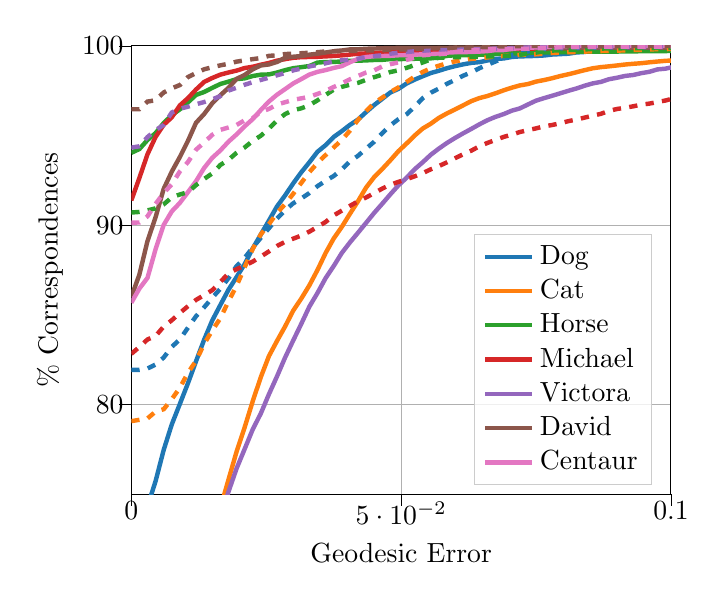
\begin{tikzpicture}

\definecolor{crimson2143940}{RGB}{214,39,40}
\definecolor{darkgray176}{RGB}{176,176,176}
\definecolor{darkorange25512714}{RGB}{255,127,14}
\definecolor{darkturquoise23190207}{RGB}{23,190,207}
\definecolor{forestgreen4416044}{RGB}{44,160,44}
\definecolor{goldenrod18818934}{RGB}{188,189,34}
\definecolor{gray127}{RGB}{127,127,127}
\definecolor{mediumpurple148103189}{RGB}{148,103,189}
\definecolor{orchid227119194}{RGB}{227,119,194}
\definecolor{sienna1408675}{RGB}{140,86,75}
\definecolor{steelblue31119180}{RGB}{31,119,180}
\definecolor{lightgray204}{RGB}{204,204,204}

\begin{axis}[
tick align=outside,
tick pos=left,
legend cell align={left},
legend style={
  fill opacity=0.8,
  draw opacity=1,
  text opacity=1,
  at={(0.8,0.3)},
  anchor=center,
  draw=lightgray204
},
xticklabel style={yshift= 5pt},
yticklabel style={xshift= 5pt},
x grid style={darkgray176},
xlabel={Geodesic Error},
xmin=0, xmax=0.10,
xtick style={color=black},
xtick = {0,0.05,0.1,0.15},
xmajorgrids,
ymajorgrids,
ytick = {40,60,70,80,90,100},
y grid style={darkgray176},
ylabel={\% Correspondences},
ymin=75, ymax=100,
ytick style={color=black}
]
\addplot [ultra thick, steelblue31119180]
table {%
0 73.3570930855583
0.0015 73.592603164312
0.003 74.3112220386222
0.0045 75.7228575135922
0.006 77.461471379082
0.0075 78.8864058221451
0.009 80.029911746404
0.0105 81.1831873160213
0.012 82.4126695477934
0.0135 83.6123376478342
0.015 84.6826935740389
0.0165 85.5444660364339
0.018 86.3928193013573
0.0195 87.0983122611407
0.021 87.82401502229
0.0225 88.6988208285774
0.024 89.4775462751514
0.0255 90.2532273932116
0.027 91.0417705547129
0.0285 91.6579873652031
0.03 92.3276077505469
0.0315 92.9472467300254
0.033 93.5036695158651
0.0345 94.089936722167
0.036 94.4577943125488
0.0375 94.9147870652092
0.039 95.2394710515672
0.0405 95.5874841544399
0.042 95.8857457242795
0.0435 96.2998015954398
0.045 96.6940356595158
0.0465 97.0417985161075
0.048 97.3960737331824
0.0495 97.5981128989376
0.051 97.8962196144792
0.0525 98.1114965300571
0.054 98.3035791278116
0.0555 98.482444129456
0.057 98.6083066000835
0.0585 98.7508515001469
0.06 98.8667866044262
0.0615 98.9660557258359
0.063 99.0488858396455
0.0645 99.0885916538088
0.066 99.1813589006121
0.0675 99.2708258633568
0.069 99.2940299291512
0.0705 99.3767941880481
0.072 99.4099485353589
0.0735 99.4198626805889
0.075 99.4364300089635
0.0765 99.4596209457223
0.078 99.5126430955028
0.0795 99.5358537881497
0.081 99.5590810051202
0.0825 99.6285585818376
0.084 99.6551025220441
0.0855 99.7446485610952
0.087 99.7512820668337
0.0885 99.7711398408861
0.09 99.7810605018436
0.0915 99.8109279561762
0.093 99.8208716109969
0.0945 99.8573988617421
0.096 99.8640290639451
0.0975 99.8706658666513
0.099 99.8706658666513
0.1005 99.8939062582789
0.102 99.903863114106
0.1035 99.9105065436649
0.105 99.9105065436649
0.1065 99.9171433463711
0.108 99.920450224678
0.1095 99.9370505100639
0.111 99.9403672596493
0.1125 99.9403672596493
0.114 99.9436807122669
0.1155 99.9436807122669
0.117 99.9470073922403
0.1185 99.9470073922403
0.12 99.9470073922403
0.1215 99.9503044578519
0.123 99.9536311378253
0.1245 99.9536311378253
0.126 99.9536311378253
0.1275 99.9536311378253
0.129 99.9635485343614
0.1305 99.9801488197473
0.132 99.9834655693327
0.1335 99.996696399075
0.135 99.996696399075
0.1365 99.996696399075
0.138 100
0.1395 100
0.141 100
0.1425 100
0.144 100
0.1455 100
0.147 100
0.1485 100
0.15 100
};
\addlegendentry{Dog}
\addplot [ultra thick, darkorange25512714]
table {%
0 52.7714062657999
0.0015 53.2133817377019
0.003 54.6202148493812
0.0045 56.6261837070809
0.006 59.1574863284341
0.0075 61.4600581901197
0.009 63.7252229712705
0.0105 66.1541015636357
0.012 68.2539976676214
0.0135 70.5114527386252
0.015 72.4194205898474
0.0165 74.2061833204971
0.018 75.7991464112943
0.0195 77.3567697377323
0.021 78.7200925567779
0.0225 80.176717847444
0.024 81.5250313619298
0.0255 82.693627258145
0.027 83.5418022255023
0.0285 84.3504758115997
0.03 85.2321215170503
0.0315 85.9041364278426
0.033 86.6429455190787
0.0345 87.498262708699
0.036 88.4398629739118
0.0375 89.2516395872194
0.039 89.8972662873064
0.0405 90.6258523175926
0.042 91.327939525673
0.0435 92.0901785711135
0.045 92.6761499864056
0.0465 93.128455133223
0.048 93.6143162692293
0.0495 94.123790544866
0.051 94.5466968614042
0.0525 94.9931609129751
0.054 95.3861235089858
0.0555 95.6560146223765
0.057 95.9822863291845
0.0585 96.2318903373849
0.06 96.4517801585735
0.0615 96.681654048647
0.063 96.9149580454908
0.0645 97.085007225017
0.066 97.2015055699254
0.0675 97.3514905114559
0.069 97.5178636720453
0.0705 97.6643990740097
0.072 97.7909078030738
0.0735 97.8675423746434
0.075 98.0040712817145
0.0765 98.0907021031679
0.078 98.1939735184826
0.0795 98.313742271881
0.081 98.4136704618421
0.0825 98.5271185903115
0.084 98.6404103378317
0.0855 98.7469752915751
0.087 98.8101830739466
0.0885 98.8534939434447
0.09 98.903444665306
0.0915 98.9566888659706
0.093 98.9966393807799
0.0945 99.0299596798736
0.096 99.0798769215151
0.0975 99.1232074377674
0.099 99.1632080042675
0.1005 99.1831384322889
0.102 99.233125798537
0.1035 99.2797799178011
0.105 99.3332473665983
0.1065 99.3632844435713
0.108 99.4198686179562
0.1095 99.4664956906352
0.111 99.4864227222041
0.1125 99.4997863595079
0.114 99.5231432100142
0.1155 99.5598036161829
0.117 99.6165444573932
0.1185 99.6365814081955
0.12 99.6665684344939
0.1215 99.6966555559891
0.123 99.7166224086323
0.1245 99.7667562908553
0.126 99.7767430571308
0.1275 99.7933865801636
0.129 99.8034166905953
0.1305 99.8100834639303
0.132 99.8333572757159
0.1335 99.8400040616669
0.135 99.8799246194816
0.1365 99.8899315192749
0.138 99.8899315192749
0.1395 99.8965782457621
0.141 99.9400556183993
0.1425 99.9500691186958
0.144 99.9567191751467
0.1455 99.963412615575
0.147 99.9700793889101
0.1485 100
0.15 100
};

\addlegendentry{Cat}
\addplot [ultra thick, forestgreen4416044]
table {%
0 94.033043572761
0.0015 94.2433889572111
0.003 94.7471356396499
0.0045 95.1309448763415
0.006 95.6916229597299
0.0075 96.1285858752191
0.009 96.4587714114379
0.0105 96.8458710722858
0.012 97.2630709058786
0.0135 97.4232255371046
0.015 97.6536176086494
0.0165 97.8704922463109
0.018 98.000893933363
0.0195 98.1409447663513
0.021 98.1843551042203
0.0225 98.3146866002387
0.024 98.3914369779126
0.0255 98.4048105523721
0.027 98.5082078438832
0.0285 98.6417187245278
0.03 98.7518929740204
0.0315 98.8087237874003
0.033 98.8720407378067
0.0345 99.0654954563503
0.036 99.095508889878
0.0375 99.1021822900656
0.039 99.12549574348
0.0405 99.165502690979
0.042 99.1688494111932
0.0435 99.1855227711799
0.045 99.2089565802594
0.0465 99.2156232735929
0.048 99.2589301269809
0.0495 99.2589301269809
0.051 99.265610153701
0.0525 99.2756168337277
0.054 99.2856536375797
0.0555 99.298986970913
0.057 99.3490607188385
0.0585 99.4391414678178
0.06 99.4692452264172
0.0615 99.4725919466314
0.063 99.4759186266048
0.0645 99.4992387333792
0.066 99.5125720667125
0.0675 99.545972501842
0.069 99.5727128096267
0.0705 99.5794062500551
0.072 99.5794062500551
0.0735 99.5994130301825
0.075 99.6295402796904
0.0765 99.6295402796904
0.078 99.6328869999045
0.0795 99.6462437972989
0.081 99.6462437972989
0.0825 99.6729774049566
0.084 99.6729774049566
0.0855 99.6729774049566
0.087 99.6729774049566
0.0885 99.6763140749599
0.09 99.6796540883199
0.0915 99.6829874216533
0.093 99.6863307850769
0.0945 99.6996775319578
0.096 99.703024252172
0.0975 99.703024252172
0.099 99.7063509321454
0.1005 99.7163510123064
0.102 99.7230110256131
0.1035 99.7230110256131
0.105 99.7563312395378
0.1065 99.7563312395378
0.108 99.7596712528979
0.1095 99.7629979328713
0.111 99.7629979328713
0.1125 99.7629979328713
0.114 99.7729846261514
0.1155 99.7897115271155
0.117 99.7897115271155
0.1185 99.8030182470091
0.12 99.8097184212809
0.1215 99.8297485115519
0.123 99.8799292144443
0.1245 99.8832725778679
0.126 99.9065859777882
0.1275 99.9132593244815
0.129 99.9132593244815
0.1305 99.9266462120856
0.132 99.9400063996642
0.1335 99.9633365031352
0.135 99.99665998664
0.1365 99.99665998664
0.138 99.99665998664
0.1395 99.99665998664
0.141 99.99665998664
0.1425 99.99665998664
0.144 99.99665998664
0.1455 99.99665998664
0.147 100
0.1485 100
0.15 100
};

\addlegendentry{Horse}
\addplot [ultra thick, crimson2143940]
table {%
0 91.3751182434072
0.0015 92.631605344031
0.003 93.9510478123857
0.0045 94.9208271990571
0.006 95.5936558497487
0.0075 96.0133657494823
0.009 96.676172163793
0.0105 97.0826387571173
0.012 97.5624913147168
0.0135 97.9854802222938
0.015 98.2057051442043
0.0165 98.3922849621175
0.018 98.5123935508633
0.0195 98.6157620042005
0.021 98.759261901114
0.0225 98.8327466923997
0.024 98.9461719719585
0.0255 99.0431646064024
0.027 99.1698939193518
0.0285 99.2565388201949
0.03 99.3299403611472
0.0315 99.3665707655599
0.033 99.3766514107212
0.0345 99.3867051269297
0.036 99.4100088910907
0.0375 99.4332992006329
0.039 99.466586367931
0.0405 99.5099137105306
0.042 99.5565042270737
0.0435 99.5765247767297
0.045 99.6031819215711
0.0465 99.6198289351967
0.048 99.6465328082779
0.0495 99.6665265027013
0.051 99.6832402861155
0.0525 99.6899138668523
0.054 99.706650871864
0.0555 99.7100110869178
0.057 99.72342501818
0.0585 99.743391764634
0.06 99.7600520992362
0.0615 99.7834058078393
0.063 99.8000627585391
0.0645 99.80338281166
0.066 99.8100295447542
0.0675 99.8133662147575
0.069 99.8133662147575
0.0705 99.8233731827267
0.072 99.82670985273
0.0735 99.8334268989352
0.075 99.8500839035341
0.0765 99.8534441185878
0.078 99.87010445319
0.0795 99.8734377865233
0.081 99.8734377865233
0.0825 99.8867445263172
0.084 99.8934649564248
0.0855 99.8934649564248
0.087 99.8967949597548
0.0885 99.9167517559995
0.09 99.9200718091204
0.0915 99.9367321437226
0.093 99.9367321437226
0.0945 99.9367321437226
0.096 99.9367321437226
0.0975 99.9434124118972
0.099 99.9600727464994
0.1005 99.9633994264728
0.102 99.9633994264728
0.1035 99.9633994264728
0.105 99.9633994264728
0.1065 99.970036229179
0.108 99.970036229179
0.1095 99.970036229179
0.111 99.9866965637812
0.1125 99.9900232437546
0.114 99.9933532470846
0.1155 99.9933532470846
0.117 99.9933532470846
0.1185 99.9933532470846
0.12 99.99666999667
0.1215 99.99666999667
0.123 99.99666999667
0.1245 99.99666999667
0.126 99.99666999667
0.1275 99.99666999667
0.129 99.99666999667
0.1305 99.99666999667
0.132 99.99666999667
0.1335 99.99666999667
0.135 99.99666999667
0.1365 100
0.138 100
0.1395 100
0.141 100
0.1425 100
0.144 100
0.1455 100
0.147 100
0.1485 100
0.15 100
};

\addlegendentry{Michael}
\addplot [ultra thick, mediumpurple148103189]
table {%
0 54.2807807797069
0.0015 56.5078104790393
0.003 58.6749368561178
0.0045 60.7560700783497
0.006 62.651172973637
0.0075 64.4946894795725
0.009 66.1715716172846
0.0105 67.766174608909
0.012 69.238770313953
0.0135 70.7454760322188
0.015 72.2617546339672
0.0165 73.7511129356525
0.018 75.1224463094033
0.0195 76.4227239795392
0.021 77.5108223707943
0.0225 78.6091317816005
0.024 79.4981461956224
0.0255 80.5682217353292
0.027 81.5663864325901
0.0285 82.6150905430054
0.03 83.5661130619301
0.0315 84.495563194923
0.033 85.4576267845771
0.0345 86.2154412905837
0.036 87.0418689634206
0.0375 87.7150825629677
0.039 88.4450993961376
0.0405 89.0310703449647
0.042 89.5718781000831
0.0435 90.1240723560339
0.045 90.6787250501776
0.0465 91.1926292818278
0.048 91.7172434801713
0.0495 92.2177627049593
0.051 92.6405293362419
0.0525 93.1134289083821
0.054 93.505681180562
0.0555 93.9251457678326
0.057 94.2696532800442
0.0585 94.5837260528373
0.06 94.8617853934031
0.0615 95.1205599860415
0.063 95.3654122741856
0.0645 95.6200442569251
0.066 95.8528463248074
0.0675 96.0388332839371
0.069 96.1917251131656
0.0705 96.3819332774377
0.072 96.5095598060885
0.0735 96.7277606710106
0.075 96.9420908965312
0.0765 97.0831575853632
0.078 97.215125166925
0.0795 97.3530755741291
0.081 97.49098756252
0.0825 97.6220421323528
0.084 97.77461246225
0.0855 97.9029728932905
0.087 97.9865297224949
0.0885 98.1355940315509
0.09 98.2188161286933
0.0915 98.3194427697131
0.093 98.3712629304263
0.0945 98.4744472995029
0.096 98.5499096757795
0.0975 98.6844396434185
0.099 98.7254871927189
0.1005 98.8260520054517
0.102 98.8881089370827
0.1035 98.9573609919338
0.105 99.0442840467842
0.1065 99.0929630968289
0.108 99.1729339852717
0.1095 99.2426815857341
0.111 99.2874883014851
0.1125 99.3187609101314
0.114 99.3604751357944
0.1155 99.4116684086412
0.117 99.45312375304
0.1185 99.4946817549838
0.12 99.5188349980588
0.1215 99.5703773817715
0.123 99.6121941445651
0.1245 99.6572048271626
0.126 99.6887141295252
0.1275 99.7094665762384
0.129 99.72342844323
0.1305 99.7337927772856
0.132 99.7713494151334
0.1335 99.7994200250625
0.135 99.827399184817
0.1365 99.8481958682777
0.138 99.8621392414916
0.1395 99.8828668698961
0.141 99.9106583679034
0.1425 99.9346254457308
0.144 99.952004032231
0.1455 99.9723222056416
0.147 99.9930222979753
0.1485 100
0.15 100
};

\addlegendentry{Victora}
\addplot [ultra thick, sienna1408675]
table {%
0 85.9880834160874
0.0015 87.2426348891096
0.003 89.11287653095
0.0045 90.4402515723271
0.006 92.0191989407481
0.0075 92.9824561403509
0.009 93.8000662032439
0.0105 94.7004303210857
0.012 95.7100297914598
0.0135 96.1966236345581
0.015 96.7957629923866
0.0165 97.2393247269116
0.018 97.6530950016551
0.0195 98.1529294935452
0.021 98.3747103608077
0.0225 98.6891757696127
0.024 98.9043363124793
0.0255 98.9606090698444
0.027 99.0996358821582
0.0285 99.3346573982125
0.03 99.3909301555776
0.0315 99.4273419397551
0.033 99.5067858325058
0.0345 99.556438265475
0.036 99.6259516716319
0.0375 99.6954650777888
0.039 99.7384971863621
0.0405 99.7980801059252
0.042 99.8047004303211
0.0435 99.8344918901026
0.045 99.8477325388944
0.0465 99.8642833498842
0.048 99.8709036742801
0.0495 99.8841443230719
0.051 99.8874544852698
0.0525 99.8874544852698
0.054 99.8874544852698
0.0555 99.8874544852698
0.057 99.8874544852698
0.0585 99.8907646474677
0.06 99.8940748096657
0.0615 99.8940748096657
0.063 99.8940748096657
0.0645 99.8940748096657
0.066 99.8940748096657
0.0675 99.8940748096657
0.069 99.8940748096657
0.0705 99.8940748096657
0.072 99.8940748096657
0.0735 99.8940748096657
0.075 99.8940748096657
0.0765 99.8940748096657
0.078 99.8940748096657
0.0795 99.8940748096657
0.081 99.8940748096657
0.0825 99.8940748096657
0.084 99.8940748096657
0.0855 99.8940748096657
0.087 99.8940748096657
0.0885 99.8940748096657
0.09 99.8940748096657
0.0915 99.8940748096657
0.093 99.8940748096657
0.0945 99.8940748096657
0.096 99.8940748096657
0.0975 99.8940748096657
0.099 99.8940748096657
0.1005 99.8940748096657
0.102 99.8940748096657
0.1035 99.8940748096657
0.105 99.8940748096657
0.1065 99.8940748096657
0.108 99.8940748096657
0.1095 99.8940748096657
0.111 99.8940748096657
0.1125 99.8940748096657
0.114 99.8940748096657
0.1155 99.9205561072493
0.117 99.9205561072493
0.1185 99.9602780536246
0.12 99.9735187024164
0.1215 99.9867593512082
0.123 99.9867593512082
0.1245 100
0.126 100
0.1275 100
0.129 100
0.1305 100
0.132 100
0.1335 100
0.135 100
0.1365 100
0.138 100
0.1395 100
0.141 100
0.1425 100
0.144 100
0.1455 100
0.147 100
0.1485 100
0.15 100
};

\addlegendentry{David}
\addplot [ultra thick, orchid227119194]
table {%
0 85.6686626746507
0.0015 86.4604125083167
0.003 87.0592149035263
0.0045 88.6560212907518
0.006 90.0099800399202
0.0075 90.7651363938789
0.009 91.2408516300732
0.0105 91.8396540252827
0.012 92.4517631403859
0.0135 93.1902860944777
0.015 93.75249500998
0.0165 94.16500332668
0.018 94.6506986027944
0.0195 95.0565535595476
0.021 95.5089820359281
0.0225 95.9115103127079
0.024 96.4204923486361
0.0255 96.8928809048569
0.027 97.272122421823
0.0285 97.5848303393214
0.03 97.9008649367931
0.0315 98.1437125748503
0.033 98.3965402528277
0.0345 98.5462408516301
0.036 98.6460412508317
0.0375 98.7658017298736
0.039 98.8656021290752
0.0405 99.0818363273453
0.042 99.2714570858283
0.0435 99.3745841650033
0.045 99.4178310046574
0.0465 99.4311377245509
0.048 99.4411177644711
0.0495 99.4710578842316
0.051 99.4777112441783
0.0525 99.5076513639388
0.054 99.5242847638057
0.0555 99.5409181636727
0.057 99.5575515635396
0.0585 99.620758483034
0.06 99.6407185628743
0.0615 99.6506986027944
0.063 99.6540252827678
0.0645 99.6773120425815
0.066 99.7039254823686
0.0675 99.7604790419162
0.069 99.7638057218896
0.0705 99.8270126413839
0.072 99.8669328010646
0.0735 99.8935462408516
0.075 99.9068529607452
0.0765 99.9168330006653
0.078 99.9600798403194
0.0795 99.9634065202928
0.081 99.9933466400532
0.0825 99.9933466400532
0.084 99.9966733200266
0.0855 99.9966733200266
0.087 99.9966733200266
0.0885 99.9966733200266
0.09 100
0.0915 100
0.093 100
0.0945 100
0.096 100
0.0975 100
0.099 100
0.1005 100
0.102 100
0.1035 100
0.105 100
0.1065 100
0.108 100
0.1095 100
0.111 100
0.1125 100
0.114 100
0.1155 100
0.117 100
0.1185 100
0.12 100
0.1215 100
0.123 100
0.1245 100
0.126 100
0.1275 100
0.129 100
0.1305 100
0.132 100
0.1335 100
0.135 100
0.1365 100
0.138 100
0.1395 100
0.141 100
0.1425 100
0.144 100
0.1455 100
0.147 100
0.1485 100
0.15 100
};

\addlegendentry{Centaur}

\addplot [ultra thick, dashed, steelblue31119180]
table {%
0 81.9310924205011
0.0015 81.9310924205011
0.003 82.0045829187697
0.0045 82.2249607859724
0.006 82.6159272328364
0.0075 83.2108089193954
0.009 83.6283616713594
0.0105 84.2795988500978
0.012 84.9209365311463
0.0135 85.418716698959
0.015 85.9499472446791
0.0165 86.4509637614316
0.018 87.0388544213631
0.0195 87.7102889659608
0.021 88.1745051486454
0.0225 88.7456656448596
0.024 89.2935094305675
0.0255 89.8247199161071
0.027 90.3625034407103
0.0285 90.8268064568538
0.03 91.2176759193243
0.0315 91.4848709448291
0.033 91.7921896882079
0.0345 92.1729755531655
0.036 92.4702843067355
0.0375 92.7373723177565
0.039 93.1082150064652
0.0405 93.5557610851295
0.042 93.8631333357502
0.0435 94.2606359775445
0.045 94.6480550621074
0.0465 95.1291819098527
0.048 95.5601181456014
0.0495 95.9075070996121
0.051 96.1780253880786
0.0525 96.6024255094601
0.054 97.0769126254265
0.0555 97.384224655224
0.057 97.6180896639047
0.0585 97.8820015870906
0.06 98.0991063015016
0.0615 98.332927873312
0.063 98.5200459746038
0.0645 98.7505843635324
0.066 98.9410391549481
0.0675 99.1280402519473
0.069 99.308327888619
0.0705 99.4820123153933
0.072 99.5755898485282
0.0735 99.6859142890519
0.075 99.7794583348439
0.0765 99.8128585623
0.078 99.8462621062653
0.0795 99.8562821664458
0.081 99.8629488331125
0.0825 99.8729789233833
0.084 99.8729789233833
0.0855 99.8830090136541
0.087 99.8963824673485
0.0885 99.9064125576193
0.09 99.9231227014377
0.0915 99.9231227014377
0.093 99.9231227014377
0.0945 99.9264660648613
0.096 99.9331427616182
0.0975 99.9331427616182
0.099 99.943172851889
0.1005 99.9532029421598
0.102 99.9532029421598
0.1035 99.9532029421598
0.105 99.9532029421598
0.1065 99.9532029421598
0.108 99.9532029421598
0.1095 99.9532029421598
0.111 99.9532029421598
0.1125 99.9632330324306
0.114 99.9632330324306
0.1155 99.9632330324306
0.117 99.9699097291876
0.1185 99.9799398194584
0.12 99.9799398194584
0.1215 99.9799398194584
0.123 99.9799398194584
0.1245 99.9799398194584
0.126 99.9799398194584
0.1275 99.9799398194584
0.129 99.9799398194584
0.1305 99.9799398194584
0.132 99.9899699097292
0.1335 99.9899699097292
0.135 99.9899699097292
0.1365 99.9899699097292
0.138 100
0.1395 100
0.141 100
0.1425 100
0.144 100
0.1455 100
0.147 100
0.1485 100
0.15 100
};
\addplot [ultra thick, dashed, darkorange25512714]
table {%
0 79.0695104752439
0.0015 79.1437265034712
0.003 79.220680976213
0.0045 79.6018207508755
0.006 79.7336546179349
0.0075 80.2928414629182
0.009 80.9329827983725
0.0105 81.766424259137
0.012 82.4313792553213
0.0135 83.3764296003184
0.015 84.1304684321768
0.0165 84.8027411973464
0.018 85.747064358888
0.0195 86.607267319321
0.021 87.6442076661863
0.0225 88.67200358882
0.024 89.4849457666955
0.0255 90.0532111761397
0.027 90.6791757170906
0.0285 91.171825272922
0.03 91.745102023647
0.0315 92.3568772378027
0.033 92.9542418732756
0.0345 93.4673066909861
0.036 93.906965219519
0.0375 94.3265968907763
0.039 94.7498045556795
0.0405 95.2606433782864
0.042 95.862431523376
0.0435 96.3571079009398
0.045 96.8051679098262
0.0465 97.108567197513
0.048 97.4190697871032
0.0495 97.6773203339521
0.051 97.9795391864349
0.0525 98.2809863724242
0.054 98.5422668517115
0.0555 98.7403035356363
0.057 98.8907691016851
0.0585 99.0227395205273
0.06 99.1309474959176
0.0615 99.2107379312389
0.063 99.2703501591244
0.0645 99.3078969156981
0.066 99.3528241391603
0.0675 99.4105489920868
0.069 99.4353536309481
0.0705 99.4683774048647
0.072 99.4913289014169
0.0735 99.5133185597697
0.075 99.5280026900593
0.0765 99.563735964218
0.078 99.6004291783194
0.0795 99.6187716315584
0.081 99.6417083524643
0.0825 99.6527092120827
0.084 99.6774620421857
0.0855 99.689381147376
0.087 99.7058953574878
0.0885 99.7223772010335
0.09 99.7324542236016
0.0915 99.7407076249052
0.093 99.7654410780219
0.0945 99.7727771452916
0.096 99.7993397474061
0.0975 99.8112551947513
0.099 99.8176775804651
0.1005 99.8259226645443
0.102 99.8479187477535
0.1035 99.8524999753316
0.105 99.8570959897534
0.1065 99.8616725992672
0.108 99.8690068428425
0.1095 99.8754227571137
0.111 99.879091289588
0.1125 99.8809140323746
0.114 99.8836642314319
0.1155 99.8909911400997
0.117 99.8937404237247
0.1185 99.9001600276351
0.12 99.912088378808
0.1215 99.912088378808
0.123 99.9139184603006
0.1245 99.9194068793889
0.126 99.9221570970436
0.1275 99.9230707562487
0.129 99.9249026816605
0.1305 99.9304003372148
0.132 99.9358942936708
0.1335 99.9377243714551
0.135 99.9432090989968
0.1365 99.9450456537833
0.138 99.9569573647778
0.1395 99.9569573647778
0.141 99.9633603882818
0.1425 99.9715934951637
0.144 99.9761682328199
0.1455 99.9844087210448
0.147 99.9899128181845
0.1485 100
0.15 100
};
\addplot [ultra thick, dashed, forestgreen4416044]
table {%
0 90.7035356785357
0.0015 90.7356803231803
0.003 90.8249713999714
0.0045 90.9339124839125
0.006 91.1589357214357
0.0075 91.5446875446875
0.009 91.7108036608036
0.0105 91.8376287001287
0.012 92.2341323466324
0.0135 92.5770556270556
0.015 92.8806574431575
0.0165 93.3539611039611
0.018 93.6397468897469
0.0195 94.0327005577005
0.021 94.3309488059488
0.0225 94.6970935220935
0.024 94.9846828971829
0.0255 95.3793901043901
0.027 95.8348187473187
0.0285 96.1938080938081
0.03 96.408117045617
0.0315 96.5135081510082
0.033 96.6903153153153
0.0345 96.9582028457028
0.036 97.2582707707707
0.0375 97.551169026169
0.039 97.7101065351065
0.0405 97.8279708279708
0.042 97.9315726440726
0.0435 98.1012333762334
0.045 98.2494637494637
0.0465 98.3905709280709
0.048 98.5370245245245
0.0495 98.635270985271
0.051 98.7692156442157
0.0525 98.9245978120978
0.054 99.0710943085943
0.0555 99.238988988989
0.057 99.3318497068497
0.0585 99.3550657800658
0.06 99.3675657800658
0.0615 99.3693514943515
0.063 99.3747086372086
0.0645 99.39078006578
0.066 99.4104354354354
0.0675 99.4157925782926
0.069 99.4336622336622
0.0705 99.460472972973
0.072 99.4854854854855
0.0735 99.5819909194909
0.075 99.6177302302302
0.0765 99.6999106249106
0.078 99.7320534820535
0.0795 99.7516963391963
0.081 99.7695534820535
0.0825 99.7766963391964
0.084 99.794565994566
0.0855 99.8249374374375
0.087 99.8463785213786
0.0885 99.84994994995
0.09 99.8570928070928
0.0915 99.8642356642357
0.093 99.8713785213785
0.0945 99.8731642356642
0.096 99.8731642356642
0.0975 99.8767356642357
0.099 99.8803070928071
0.1005 99.8946053196053
0.102 99.896391033891
0.1035 99.9160464035464
0.105 99.9196178321179
0.1065 99.9446303446303
0.108 99.9517732017732
0.1095 99.9571303446304
0.111 99.9571303446304
0.1125 99.9732142857143
0.114 99.975
0.1155 99.9785714285714
0.117 99.9839285714286
0.1185 99.9875
0.12 99.9910714285714
0.1215 99.9910714285714
0.123 99.9928571428571
0.1245 99.9928571428571
0.126 99.9982142857143
0.1275 100
0.129 100
0.1305 100
0.132 100
0.1335 100
0.135 100
0.1365 100
0.138 100
0.1395 100
0.141 100
0.1425 100
0.144 100
0.1455 100
0.147 100
0.1485 100
0.15 100
};
\addplot [ultra thick, dashed, crimson2143940]
table {%
0 82.8216899292996
0.0015 83.2058394473594
0.003 83.6241160340079
0.0045 83.8153282752127
0.006 84.3435341747518
0.0075 84.6945801199768
0.009 85.1019422696843
0.0105 85.4776385293923
0.012 85.8323347560135
0.0135 86.0999983071133
0.015 86.372754478914
0.0165 86.8311720315121
0.018 87.3051467173633
0.0195 87.5423483562087
0.021 87.7442964189842
0.0225 87.9658468876969
0.024 88.2457563593707
0.0255 88.5335067407806
0.027 88.8372708896843
0.0285 89.0692421408393
0.03 89.2450205894764
0.0315 89.4187573295854
0.033 89.6373367799273
0.0345 89.9011457828938
0.036 90.1757467024618
0.0375 90.540222093595
0.039 90.8068613222536
0.0405 91.0708337530166
0.042 91.3245588398071
0.0435 91.5418079401854
0.045 91.7829945610806
0.0465 92.0371320450529
0.048 92.2553188179808
0.0495 92.4103124487021
0.051 92.562430095293
0.0525 92.7204954623873
0.054 92.8971937748744
0.0555 93.1141147889398
0.057 93.2939555689015
0.0585 93.503370086244
0.06 93.732227276726
0.0615 93.9537003983255
0.063 94.1530898947933
0.0645 94.3963530995321
0.066 94.5844161103526
0.0675 94.7541848431315
0.069 94.9181957641153
0.0705 95.0502264989765
0.072 95.1903220264438
0.0735 95.2999433559307
0.075 95.3945130470747
0.0765 95.5083786137908
0.078 95.5849261570319
0.0795 95.6802537641237
0.081 95.7989916606853
0.0825 95.8878260769159
0.084 95.9958437392715
0.0855 96.103537578074
0.087 96.2055351080913
0.0885 96.3685708871454
0.09 96.4764443733926
0.0915 96.5453311873151
0.093 96.6253778304054
0.0945 96.7186166359395
0.096 96.7771950523909
0.0975 96.8620153476561
0.099 96.9506445446387
0.1005 97.0705058929194
0.102 97.1879193050659
0.1035 97.2994334014879
0.105 97.3908132307092
0.1065 97.4593108408014
0.108 97.5337487876734
0.1095 97.6616365805801
0.111 97.7236651882648
0.1125 97.8276476529156
0.114 97.9241782003679
0.1155 98.0333447666767
0.117 98.1114418389967
0.1185 98.2097158416412
0.12 98.3021340581478
0.1215 98.3846035576397
0.123 98.5216641093732
0.1245 98.6120837724141
0.126 98.717261566227
0.1275 98.8233727805865
0.129 98.961503137701
0.1305 99.0801511840256
0.132 99.1555695002671
0.1335 99.2687912083751
0.135 99.3469167697517
0.1365 99.4406476415933
0.138 99.4913721400845
0.1395 99.59125427067
0.141 99.6843965205802
0.1425 99.7529300937787
0.144 99.8174950282333
0.1455 99.8823754196331
0.147 99.9371821367986
0.1485 100
0.15 100
};
\addplot [ultra thick, dashed, mediumpurple148103189]
table {%
0 94.3223481056814
0.0015 94.3973587223587
0.003 94.9103012103013
0.0045 95.2914323414324
0.006 95.5876892043559
0.0075 96.2802241635575
0.009 96.4908977158977
0.0105 96.6060689477356
0.012 96.7409507992842
0.0135 96.864460672794
0.015 97.0144750811417
0.0165 97.1948076864743
0.018 97.50091000091
0.0195 97.6623183789851
0.021 97.8267472017472
0.0225 97.9729926896594
0.024 98.0957472624139
0.0255 98.2230556313889
0.027 98.3564230897564
0.0285 98.4806875056875
0.03 98.6307246640579
0.0315 98.7292239208906
0.033 98.850455000455
0.0345 98.9322921406255
0.036 99.02549670883
0.0375 99.1300785634119
0.039 99.1944785694785
0.0405 99.2209967543301
0.042 99.2808566141899
0.0435 99.3717960384627
0.045 99.42407331574
0.0465 99.4725642308976
0.048 99.5604513604514
0.0495 99.6104543937877
0.051 99.6513680347014
0.0525 99.6953210786544
0.054 99.7021415354749
0.0555 99.7286612369946
0.057 99.7544218460885
0.0585 99.7642756392756
0.06 99.7756438256438
0.0615 99.7870135286802
0.063 99.7961074711074
0.0645 99.8074748991415
0.066 99.8233862650529
0.0675 99.8468877968878
0.069 99.8499180999181
0.0705 99.8688658355325
0.072 99.8900794734128
0.0735 99.8999302332635
0.075 99.9006885673552
0.0765 99.9014469014469
0.078 99.9029635696302
0.0795 99.9112976612976
0.081 99.9279658446325
0.0825 99.9287234203901
0.084 99.9302385719053
0.0855 99.9309961476628
0.087 99.9309961476628
0.0885 99.9332696332697
0.09 99.934786301453
0.0915 99.9355446355447
0.093 99.9355446355447
0.0945 99.9363029696363
0.096 99.9378196378197
0.0975 99.9385779719113
0.099 99.9408529741864
0.1005 99.9423696423697
0.102 99.9454029787363
0.1035 99.9476779810113
0.105 99.9567772317773
0.1065 99.9575355658689
0.108 99.9575355658689
0.1095 99.9590522340523
0.111 99.9590522340523
0.1125 99.9598105681439
0.114 99.9613272363273
0.1155 99.9727014893681
0.117 99.9734598234598
0.1185 99.9734598234598
0.12 99.9742181575514
0.1215 99.9757348257348
0.123 99.9757348257348
0.1245 99.9848340765007
0.126 99.9848340765007
0.1275 99.9855924105924
0.129 99.9878674128674
0.1305 99.9901424151424
0.132 99.9901424151424
0.1335 99.9901424151424
0.135 99.9901424151424
0.1365 99.990900749234
0.138 99.9916590833257
0.1395 99.9916590833257
0.141 99.9916590833257
0.1425 100
0.144 100
0.1455 100
0.147 100
0.1485 100
0.15 100
};
\addplot [ultra thick, dashed, sienna1408675]
table {%
0 96.4633333333333
0.0015 96.4633333333333
0.003 96.89
0.0045 96.9633333333333
0.006 97.3966666666666
0.0075 97.6299999999999
0.009 97.8133333333333
0.0105 98.2566666666667
0.012 98.4833333333333
0.0135 98.69
0.015 98.8066666666667
0.0165 98.91
0.018 98.9966666666667
0.0195 99.1166666666667
0.021 99.1866666666667
0.0225 99.2566666666667
0.024 99.3166666666667
0.0255 99.4366666666667
0.027 99.4733333333333
0.0285 99.54
0.03 99.56
0.0315 99.5866666666667
0.033 99.6133333333333
0.0345 99.6433333333333
0.036 99.6866666666667
0.0375 99.6966666666667
0.039 99.71
0.0405 99.7133333333333
0.042 99.7133333333333
0.0435 99.74
0.045 99.7466666666667
0.0465 99.76
0.048 99.77
0.0495 99.79
0.051 99.8033333333333
0.0525 99.83
0.054 99.83
0.0555 99.8466666666667
0.057 99.87
0.0585 99.88
0.06 99.8933333333333
0.0615 99.9
0.063 99.9033333333333
0.0645 99.9166666666667
0.066 99.9266666666667
0.0675 99.9666666666667
0.069 99.9666666666667
0.0705 99.9666666666667
0.072 99.9833333333333
0.0735 100
0.075 100
0.0765 100
0.078 100
0.0795 100
0.081 100
0.0825 100
0.084 100
0.0855 100
0.087 100
0.0885 100
0.09 100
0.0915 100
0.093 100
0.0945 100
0.096 100
0.0975 100
0.099 100
0.1005 100
0.102 100
0.1035 100
0.105 100
0.1065 100
0.108 100
0.1095 100
0.111 100
0.1125 100
0.114 100
0.1155 100
0.117 100
0.1185 100
0.12 100
0.1215 100
0.123 100
0.1245 100
0.126 100
0.1275 100
0.129 100
0.1305 100
0.132 100
0.1335 100
0.135 100
0.1365 100
0.138 100
0.1395 100
0.141 100
0.1425 100
0.144 100
0.1455 100
0.147 100
0.1485 100
0.15 100
};
\addplot [ultra thick, dashed, orchid227119194]
table {%
0 90.14
0.0015 90.1466666666667
0.003 90.49
0.0045 91.1866666666667
0.006 91.7866666666666
0.0075 92.2766666666666
0.009 92.9933333333333
0.0105 93.52
0.012 94.2066666666667
0.0135 94.61
0.015 95.0366666666666
0.0165 95.31
0.018 95.4466666666667
0.0195 95.5833333333333
0.021 95.8466666666667
0.0225 95.9633333333333
0.024 96.32
0.0255 96.48
0.027 96.7266666666666
0.0285 96.8533333333334
0.03 96.9866666666667
0.0315 97.07
0.033 97.1566666666667
0.0345 97.3166666666666
0.036 97.4766666666666
0.0375 97.7033333333333
0.039 97.9033333333333
0.0405 98.13
0.042 98.3166666666667
0.0435 98.51
0.045 98.6333333333334
0.0465 98.8466666666667
0.048 98.9733333333333
0.0495 99.0766666666667
0.051 99.2133333333333
0.0525 99.3366666666667
0.054 99.47
0.0555 99.51
0.057 99.5333333333333
0.0585 99.5666666666667
0.06 99.6533333333333
0.0615 99.7
0.063 99.7633333333333
0.0645 99.78
0.066 99.81
0.0675 99.8133333333333
0.069 99.82
0.0705 99.8266666666667
0.072 99.8333333333333
0.0735 99.8366666666667
0.075 99.86
0.0765 99.8666666666667
0.078 99.89
0.0795 99.9266666666667
0.081 99.9333333333333
0.0825 99.9366666666667
0.084 99.9366666666667
0.0855 99.95
0.087 99.95
0.0885 99.95
0.09 99.95
0.0915 99.95
0.093 99.95
0.0945 99.95
0.096 99.9533333333333
0.0975 99.9566666666667
0.099 99.9566666666667
0.1005 99.96
0.102 99.96
0.1035 99.9766666666667
0.105 99.98
0.1065 99.98
0.108 99.98
0.1095 99.9833333333333
0.111 99.9833333333333
0.1125 99.9833333333333
0.114 99.9833333333333
0.1155 99.9833333333333
0.117 99.9833333333333
0.1185 99.9833333333333
0.12 100
0.1215 100
0.123 100
0.1245 100
0.126 100
0.1275 100
0.129 100
0.1305 100
0.132 100
0.1335 100
0.135 100
0.1365 100
0.138 100
0.1395 100
0.141 100
0.1425 100
0.144 100
0.1455 100
0.147 100
0.1485 100
0.15 100
};
\end{axis}

\end{tikzpicture}
}
    \caption{PCK for seven different classes of TOSCA.
    We plot our method with solid lines and IsoMuSh~\cite{Gao2021} with dashed lines. 
    }
    \label{fig:SMAL_Variation}
\end{figure}

\begin{table}[h]
    \centering
    \resizebox{\linewidth}{!}{
    \begin{tabular}{|c|ccccccc|}
    \hline 
    & Dog & Cat & Horse & Michael & Victoria & David & Centaur \\ \hline
    Ours    & 0.957 & 0.917          & \textbf{0.990} & \textbf{0.992} & 0.912 & 0.989 & 0.983 \\ 
    IsoMush & \textbf{0.959} & \textbf{0.959} & 0.981         & 0.939 & \textbf{0.991} & \textbf{0.996} & \textbf{0.984} \\ \hline
\end{tabular}
}
    \caption{AUC across seven different classes of TOSCA. 
    }
    \label{Table:SMAL_variation}
\end{table}




















\subsection{Influence of Descriptors}


We ablate the need for left-right indicators when using HKS descriptors for initialisation. %
Fig.~\ref{fig:noLR} contains results on the cat class of TOSCA.
Without left-right indicators, we observe flips in the matchings on TOSCA and partial flips on FAUST for inter-class instances. %
This is expected since both our method and IsoMuSh exploit intrinsic properties of the shapes, which are invariant to such symmetric flips. 

\begin{figure}[h]
    \centering
    \resizebox{0.5\linewidth}{!}{
    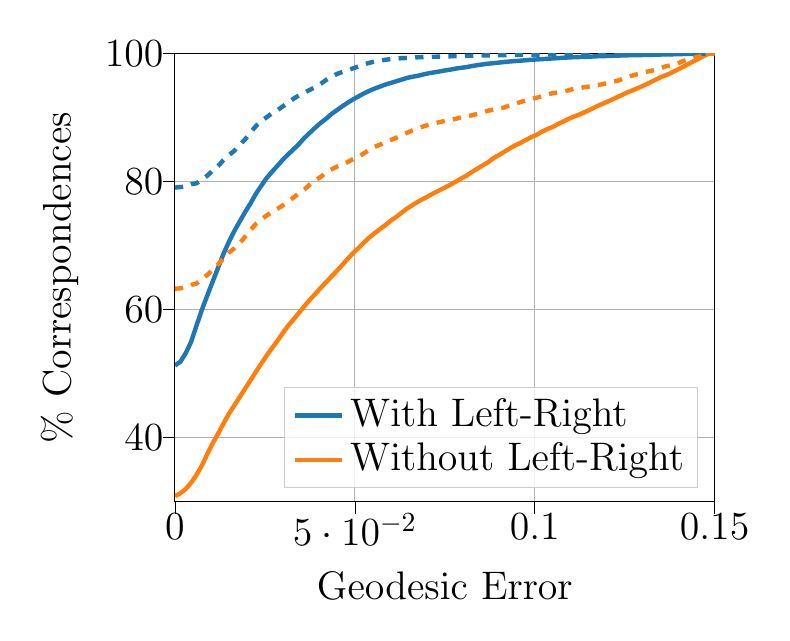
\begin{tikzpicture}

\definecolor{crimson2143940}{RGB}{214,39,40}
\definecolor{darkgray176}{RGB}{176,176,176}
\definecolor{darkorange25512714}{RGB}{255,127,14}
\definecolor{forestgreen4416044}{RGB}{44,160,44}
\definecolor{steelblue31119180}{RGB}{31,119,180}
\definecolor{lightgray204}{RGB}{204,204,204}

\Large
\begin{axis}[
legend cell align={left},
legend style={
  fill opacity=0.8,
  draw opacity=1,
  text opacity=1,
  at={(0.97,0.03)},
  anchor=south east,
  draw=lightgray204
},
tick align=outside,
tick pos=left,
x grid style={darkgray176},
xtick = {0,0.05,0.1,0.15},
xlabel={Geodesic Error},
xmin=0, xmax=0.15,
xtick style={color=black},
xticklabel style={yshift= 5pt},
xmajorgrids,
ymajorgrids,
yticklabel style={xshift= 5pt},
y grid style={darkgray176},
ylabel={\% Correspondences},
ymin=30, ymax=100,
ytick style={color=black}
]
\addplot [ultra thick, steelblue31119180]
table {%
0 51.2827555390533
0.0015 51.8641372208934
0.003 53.2146159655153
0.0045 54.9806382405994
0.006 57.5146025317151
0.0075 60.0077856895293
0.009 62.2242898780877
0.0105 64.4028120915058
0.012 66.5613921234063
0.0135 68.7289465041221
0.015 70.5978661899041
0.0165 72.2701509840696
0.018 73.7657422983166
0.0195 75.2364019588098
0.021 76.5895894445652
0.0225 78.0961042728416
0.024 79.3599204131689
0.0255 80.565712515973
0.027 81.5449937514256
0.0285 82.4800868600155
0.03 83.4303835051003
0.0315 84.2809246820583
0.033 85.0615693434214
0.0345 85.8897366138886
0.036 86.8285148833775
0.0375 87.6282134975959
0.039 88.4200562405174
0.0405 89.1711195013369
0.042 89.8093719119894
0.0435 90.549537342114
0.045 91.1498265445945
0.0465 91.7545031478986
0.048 92.3102448944225
0.0495 92.8378606567253
0.051 93.2893909734178
0.0525 93.7646146635959
0.054 94.1660987558939
0.0555 94.5203149535873
0.057 94.8399191615949
0.0585 95.1568627220012
0.06 95.4059253437614
0.0615 95.6612266571517
0.063 95.9238159659513
0.0645 96.1864891910602
0.066 96.3673276048486
0.0675 96.5236294751415
0.069 96.7261918561814
0.0705 96.9096410762237
0.072 97.0495961686294
0.0735 97.1931381524204
0.075 97.3493913029419
0.0765 97.4765878627066
0.078 97.6429356159051
0.0795 97.7664438653261
0.081 97.8736574395139
0.0825 98.0318578047599
0.084 98.1764065379189
0.0855 98.2891758744252
0.087 98.4108905798865
0.0885 98.4872071879577
0.09 98.5826375265531
0.0915 98.6698075988052
0.093 98.7524639437443
0.0945 98.8170101170457
0.096 98.8787447655987
0.0975 98.947842144327
0.099 99.0178790993535
0.1005 99.0714371161864
0.102 99.1204759060856
0.1035 99.1687286116406
0.105 99.2324616730183
0.1065 99.2779569428163
0.108 99.3397469513088
0.1095 99.3906720609429
0.111 99.4224652531733
0.1125 99.448871149192
0.114 99.4770505330181
0.1155 99.5152549382668
0.117 99.5625720820572
0.1185 99.5789450218972
0.12 99.6098882483429
0.1215 99.6471732513815
0.123 99.6626280416896
0.1245 99.7026838798648
0.126 99.7226868241501
0.1275 99.7399697710862
0.129 99.7527210027383
0.1305 99.769995827692
0.132 99.7917734316924
0.1335 99.8053954570241
0.135 99.8390259623233
0.1365 99.8581309500769
0.138 99.8717538435083
0.1395 99.8944714971738
0.141 99.9172683508007
0.1425 99.9327394912886
0.144 99.9490933303313
0.1455 99.9600254218557
0.147 99.9791076411799
0.1485 100
0.15 100
};
\addlegendentry{With Left-Right}
\addplot [ultra thick, darkorange25512714]
table {%
0 30.8864013818146
0.0015 31.3228911230655
0.003 32.0042701802558
0.0045 32.9805270466876
0.006 34.2026321595216
0.0075 35.6839164914589
0.009 37.458313192461
0.0105 39.1481346636783
0.012 40.6454369335862
0.0135 42.2248943899164
0.015 43.7578306157743
0.0165 45.0573616792517
0.018 46.3436839854523
0.0195 47.6560882537004
0.021 48.9596869155032
0.0225 50.3027046752211
0.024 51.5686465903498
0.0255 52.845318758874
0.027 54.0125607781556
0.0285 55.1522410601754
0.03 56.3677777391881
0.0315 57.5128841148021
0.033 58.5092758727202
0.0345 59.5225796506218
0.036 60.5602142256785
0.0375 61.5492043458269
0.039 62.4530560742832
0.0405 63.4029900967566
0.042 64.2865342945899
0.0435 65.1603898250192
0.045 66.0505618738915
0.0465 66.9746949643089
0.048 67.9183410572697
0.0495 68.8227379810735
0.051 69.630824422822
0.0525 70.4582982844795
0.054 71.2523511597591
0.0555 71.9386383338911
0.057 72.5835809059024
0.0585 73.2080315641417
0.06 73.9086890462388
0.0615 74.4850139083331
0.063 75.1435008856221
0.0645 75.7774064462289
0.066 76.3155157209705
0.0675 76.8545341832699
0.069 77.2977061542876
0.0705 77.7457450908665
0.072 78.2199403626026
0.0735 78.6411115702198
0.075 79.055747303738
0.0765 79.5081981374898
0.078 79.9671784227686
0.0795 80.4757214040484
0.081 80.9153083785992
0.0825 81.4810116792612
0.084 82.0090490594881
0.0855 82.502068654266
0.087 83.0063415817128
0.0885 83.6430205669229
0.09 84.1199631074617
0.0915 84.6432107119071
0.093 85.1495485773543
0.0945 85.635644569429
0.096 86.0389197230268
0.0975 86.4800179249469
0.099 86.9305216703729
0.1005 87.2947793066458
0.102 87.7891482385605
0.1035 88.1929931961544
0.105 88.5325875885285
0.1065 88.9946512590125
0.108 89.3933716224593
0.1095 89.8074862512947
0.111 90.1721705785302
0.1125 90.4940091516515
0.114 90.8751571754104
0.1155 91.2588840625922
0.117 91.6793207261531
0.1185 92.0633832265236
0.12 92.4236134653785
0.1215 92.7943290348873
0.123 93.202902040884
0.1245 93.5982003073131
0.126 93.9812169742051
0.1275 94.3146090377232
0.129 94.6918770245565
0.1305 95.0519308509003
0.132 95.4613384889146
0.1335 95.880425196154
0.135 96.294433426717
0.1365 96.6239159470051
0.138 96.9984225089091
0.1395 97.419678444136
0.141 97.8565808702181
0.1425 98.297323639062
0.144 98.7522214469978
0.1455 99.1577983152942
0.147 99.6219074422467
0.1485 100
0.15 100
};
\addlegendentry{Without Left-Right}

\addplot [ultra thick,dashed, steelblue31119180]
table {%
0 79.0695104752439
0.0015 79.1437265034712
0.003 79.220680976213
0.0045 79.6018207508755
0.006 79.7336546179349
0.0075 80.2928414629182
0.009 80.9329827983725
0.0105 81.766424259137
0.012 82.4313792553213
0.0135 83.3764296003184
0.015 84.1304684321768
0.0165 84.8027411973464
0.018 85.747064358888
0.0195 86.607267319321
0.021 87.6442076661863
0.0225 88.67200358882
0.024 89.4849457666955
0.0255 90.0532111761397
0.027 90.6791757170906
0.0285 91.171825272922
0.03 91.745102023647
0.0315 92.3568772378027
0.033 92.9542418732756
0.0345 93.4673066909861
0.036 93.906965219519
0.0375 94.3265968907763
0.039 94.7498045556795
0.0405 95.2606433782864
0.042 95.862431523376
0.0435 96.3571079009398
0.045 96.8051679098262
0.0465 97.108567197513
0.048 97.4190697871032
0.0495 97.6773203339521
0.051 97.9795391864349
0.0525 98.2809863724242
0.054 98.5422668517115
0.0555 98.7403035356363
0.057 98.8907691016851
0.0585 99.0227395205273
0.06 99.1309474959176
0.0615 99.2107379312389
0.063 99.2703501591244
0.0645 99.3078969156981
0.066 99.3528241391603
0.0675 99.4105489920868
0.069 99.4353536309481
0.0705 99.4683774048647
0.072 99.4913289014169
0.0735 99.5133185597697
0.075 99.5280026900593
0.0765 99.563735964218
0.078 99.6004291783194
0.0795 99.6187716315584
0.081 99.6417083524643
0.0825 99.6527092120827
0.084 99.6774620421857
0.0855 99.689381147376
0.087 99.7058953574878
0.0885 99.7223772010335
0.09 99.7324542236016
0.0915 99.7407076249052
0.093 99.7654410780219
0.0945 99.7727771452916
0.096 99.7993397474061
0.0975 99.8112551947513
0.099 99.8176775804651
0.1005 99.8259226645443
0.102 99.8479187477535
0.1035 99.8524999753316
0.105 99.8570959897534
0.1065 99.8616725992672
0.108 99.8690068428425
0.1095 99.8754227571137
0.111 99.879091289588
0.1125 99.8809140323746
0.114 99.8836642314319
0.1155 99.8909911400997
0.117 99.8937404237247
0.1185 99.9001600276351
0.12 99.912088378808
0.1215 99.912088378808
0.123 99.9139184603006
0.1245 99.9194068793889
0.126 99.9221570970436
0.1275 99.9230707562487
0.129 99.9249026816605
0.1305 99.9304003372148
0.132 99.9358942936708
0.1335 99.9377243714551
0.135 99.9432090989968
0.1365 99.9450456537833
0.138 99.9569573647778
0.1395 99.9569573647778
0.141 99.9633603882818
0.1425 99.9715934951637
0.144 99.9761682328199
0.1455 99.9844087210448
0.147 99.9899128181845
0.1485 100
0.15 100
};
\addplot [ultra thick, dashed, darkorange25512714]
table {%
0 63.2872061937912
0.0015 63.3257937691775
0.003 63.5029985820476
0.0045 63.8562793475192
0.006 64.0958773355048
0.0075 64.7714969227338
0.009 65.4335776123682
0.0105 66.2871089856193
0.012 67.0868314975317
0.0135 67.9892635729781
0.015 68.8987999157729
0.0165 69.5674408369531
0.018 70.3880018268584
0.0195 71.3866325442277
0.021 72.4122506703419
0.0225 73.3941570418858
0.024 74.0796982791265
0.0255 74.7184548593408
0.027 75.237531860262
0.0285 75.7481397018424
0.03 76.3031991308835
0.0315 76.919296037866
0.033 77.5256083348013
0.0345 78.1919496488265
0.036 78.7640684466356
0.0375 79.5431602141617
0.039 80.1836661898661
0.0405 80.7242855030505
0.042 81.414376829219
0.0435 81.9033023502117
0.045 82.3261372349325
0.0465 82.6685313499164
0.048 83.051857741486
0.0495 83.5075672761412
0.051 83.9029598353477
0.0525 84.3945439790794
0.054 84.9888725552633
0.0555 85.4344891998671
0.057 85.7684480314269
0.0585 86.1592022787808
0.06 86.496368577331
0.0615 86.8326808438198
0.063 87.2298518290145
0.0645 87.6173582115383
0.066 87.987116199531
0.0675 88.2707211953121
0.069 88.6071331770038
0.0705 88.8606238649692
0.072 89.0835010044758
0.0735 89.2777466156127
0.075 89.4796785712188
0.0765 89.6335042748515
0.078 89.7994238142735
0.0795 90.0424849526938
0.081 90.175163217196
0.0825 90.3501915210532
0.084 90.5666072069471
0.0855 90.7868414237197
0.087 91.0677846607635
0.0885 91.2538411447847
0.09 91.4198614422892
0.0915 91.5586831563131
0.093 91.9073067363329
0.0945 92.1407853169098
0.096 92.4153076761621
0.0975 92.6781445040729
0.099 92.8967610724501
0.1005 93.0823564694153
0.102 93.3323113726001
0.1035 93.5873237509984
0.105 93.8123242964938
0.1065 93.9258950664783
0.108 94.0567754682418
0.1095 94.2716490198321
0.111 94.5220404820941
0.1125 94.5948345226282
0.114 94.770697682393
0.1155 94.8577862526481
0.117 95.0422429973284
0.1185 95.1672324331746
0.12 95.3636353745629
0.1215 95.5720722082164
0.123 95.7469947459563
0.1245 96.0561514092007
0.126 96.3315416515112
0.1275 96.6433986115411
0.129 96.8172310475166
0.1305 97.0834559942452
0.132 97.252853150831
0.1335 97.4270176326627
0.135 97.6962965714717
0.1365 98.0069385419717
0.138 98.1708406811048
0.1395 98.3993046110812
0.141 98.7685846674754
0.1425 99.0265916401134
0.144 99.286195611681
0.1455 99.4983256173369
0.147 99.6782215084182
0.1485 100
0.15 100
};
\end{axis}

\end{tikzpicture}

    }
    \caption{PCK with and without left-right descriptors.
    We plot our method with solid lines and IsoMuSh~\cite{Gao2021} with dashed lines. }
    \label{fig:noLR}
\end{figure}



\subsection{Noise Perturbation} 


We investigate the robustness of our approach to noise. 
To that end, we analyse the effect of adding synthetic perturbations to the shapes. 
Specifically, for each FAUST mesh, we add a Gaussian-distributed offset along the vertex normal to each vertex position.
This ensures the meshed structure of the shape does not change. 
Fig.~\ref{fig:noisy} visualises the amount of noise we experiment with.
Fig.~\ref{fig:NoiseVariation} shows that our method is significantly more robust to noise than IsoMuSh. 

\begin{figure}[h]
    \centering
    \includegraphics[width=.3\linewidth]{SupplimentFigures/noisy/shape_001.png}
    \quad
    \includegraphics[width=.3\linewidth]{SupplimentFigures/noisy/shape_002.png}
    \caption{Example of perturbing the geometry on FAUST, with the noise variance set to $0.01$ (left) and $0.02$ (right).}
    \label{fig:noisy}
\end{figure}

\begin{figure}[h]%
    \centering
    \resizebox{0.5\linewidth}{!}{
    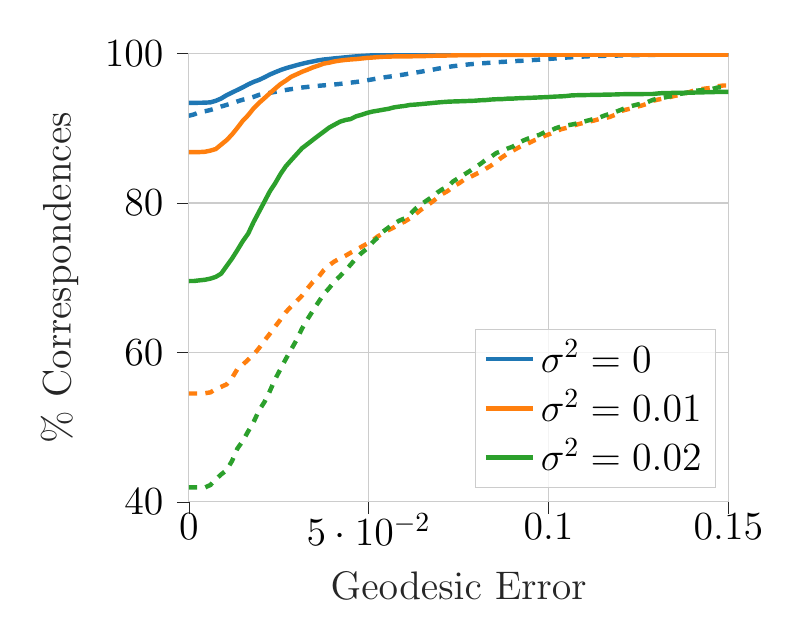
\begin{tikzpicture}

\definecolor{darkorange25512714}{RGB}{255,127,14}
\definecolor{darkslategray38}{RGB}{38,38,38}
\definecolor{forestgreen4416044}{RGB}{44,160,44}
\definecolor{lightgray204}{RGB}{204,204,204}
\definecolor{steelblue31119180}{RGB}{31,119,180}

\Large
\begin{axis}[
axis line style={lightgray204},
legend cell align={left},
legend style={
  fill opacity=0.8,
  draw opacity=1,
  text opacity=1,
  at={(0.53,0.03)},
  anchor=south west,
  draw=lightgray204
},
tick align=outside,
tick pos=left,
xtick = {0,0.05,0.10,0.15},
ytick = {40,60,80,100},
x grid style={lightgray204},
xlabel=\textcolor{darkslategray38}{Geodesic Error},
xmajorgrids,
xmin=0, xmax=0.15,
xtick style={color=darkslategray38},
xticklabel style={yshift= 5pt},
y grid style={lightgray204},
ylabel=\textcolor{darkslategray38}{\% Correspondences},
ymajorgrids,
ymin=40, ymax=100,
ytick style={color=darkslategray38}
]
\addplot [ultra thick, steelblue31119180]
table {%
0 93.4019477644976
0.0015 93.4021691013723
0.003 93.4074811863656
0.0045 93.4229747675963
0.006 93.4645861000443
0.0075 93.6702080566622
0.009 93.9803010181496
0.0105 94.4156706507304
0.012 94.7726870296591
0.0135 95.1188579017264
0.015 95.4712262062859
0.0165 95.8612217795485
0.018 96.199203187251
0.0195 96.4645861000443
0.021 96.8025675077468
0.0225 97.1790615316512
0.024 97.4922532093847
0.0255 97.7833111996458
0.027 98.0336432049579
0.0285 98.2386011509517
0.03 98.4420097388225
0.0315 98.6250553342187
0.033 98.7990261177512
0.0345 98.9389110225763
0.036 99.0894200973882
0.0375 99.1963258078796
0.039 99.2682602921646
0.0405 99.3530323151836
0.042 99.4156706507303
0.0435 99.4873837981407
0.045 99.5559982293049
0.0465 99.6177512173528
0.048 99.6757414785303
0.0495 99.7153607791058
0.051 99.7563081009296
0.0525 99.7886232846392
0.054 99.8065515714918
0.0555 99.8247011952191
0.057 99.839973439575
0.0585 99.847941567065
0.06 99.8601150951748
0.0615 99.8634351482957
0.063 99.8691899070385
0.0645 99.8747233289066
0.066 99.881584772023
0.0675 99.8851261620185
0.069 99.8860115095174
0.0705 99.8906595838866
0.072 99.893536963258
0.0735 99.8968570163789
0.075 99.9026117751217
0.0765 99.9052678176184
0.078 99.9061531651173
0.0795 99.9065958388667
0.081 99.9096945551128
0.0825 99.9163346613546
0.084 99.9196547144754
0.0855 99.9225320938468
0.087 99.9260734838424
0.0885 99.9267374944666
0.09 99.9280655157149
0.0915 99.9285081894643
0.093 99.9285081894643
0.0945 99.9293935369632
0.096 99.9318282425852
0.0975 99.9322709163346
0.099 99.9324922532093
0.1005 99.9329349269588
0.102 99.935148295706
0.1035 99.9393536963258
0.105 99.9393536963258
0.1065 99.9424524125719
0.108 99.9424524125719
0.1095 99.9431164231961
0.111 99.9446657813191
0.1125 99.945551128818
0.114 99.9459938025675
0.1155 99.9464364763169
0.117 99.9475431606906
0.1185 99.9510845506861
0.12 99.951969898185
0.1215 99.9528552456839
0.123 99.9532979194334
0.1245 99.954404603807
0.126 99.9552899513059
0.1275 99.95595396193
0.129 99.9561752988048
0.1305 99.9572819831784
0.132 99.9581673306773
0.1335 99.9586100044267
0.135 99.9586100044267
0.1365 99.9586100044267
0.138 99.9586100044267
0.1395 99.9588313413014
0.141 99.9590526781762
0.1425 99.9610447100487
0.144 99.9612660469234
0.1455 99.9612660469234
0.147 99.9612660469234
0.1485 99.9614873837981
0.15 99.9614873837981
};
\addlegendentry{$\sigma^2=0$}
\addplot [ultra thick, steelblue31119180, dashed, forget plot]
table {%
0 91.6682988047811
0.0015 91.8573559096949
0.003 92.1534072598499
0.0045 92.2699092518816
0.006 92.4444147853034
0.0075 92.6561049136786
0.009 92.9077742363879
0.0105 93.1210084108013
0.012 93.3243311199647
0.0135 93.5868308986276
0.015 93.820584329349
0.0165 93.9781297034086
0.018 94.1964696768483
0.0195 94.4627162461269
0.021 94.6034532979197
0.0225 94.7307100486944
0.024 94.866814962373
0.0255 95.0051606905713
0.027 95.1204501992035
0.0285 95.2372828685262
0.03 95.3412611775124
0.0315 95.4511212926075
0.033 95.5294431164233
0.0345 95.6038857901726
0.036 95.6777923860115
0.0375 95.7374249667994
0.039 95.7899269588312
0.0405 95.8569738822487
0.042 95.9315214696767
0.0435 96.0127498893314
0.045 96.1053359893757
0.0465 96.1861797255421
0.048 96.2939172200086
0.0495 96.4090708277998
0.051 96.5369482071712
0.0525 96.667708277999
0.054 96.7856184152279
0.0555 96.8869433377599
0.057 96.9861580345284
0.0585 97.0896980965028
0.06 97.2038640991587
0.0615 97.3278587870737
0.063 97.4450053120849
0.0645 97.5617963700753
0.066 97.6993984063747
0.0675 97.8068924302792
0.069 97.9534856131036
0.0705 98.0742872952638
0.072 98.1945254537411
0.0735 98.304020362993
0.075 98.389926516158
0.0765 98.4715276671097
0.078 98.5557777777782
0.0795 98.6202328463926
0.081 98.6725170429397
0.0825 98.7215692784422
0.084 98.7778260292168
0.0855 98.8353948649849
0.087 98.8738255865432
0.0885 98.9146892430284
0.09 98.9640730411692
0.0915 99.0067091633472
0.093 99.0378357680395
0.0945 99.0886843736173
0.096 99.1400743691906
0.0975 99.1785024347063
0.099 99.2314125719351
0.1005 99.2930987162467
0.102 99.3449207613994
0.1035 99.395184594954
0.105 99.457755201417
0.1065 99.503370075255
0.108 99.5598401947769
0.1095 99.5897419212044
0.111 99.6271522797702
0.1125 99.6498583444005
0.114 99.6764285081898
0.1155 99.6943700752548
0.117 99.7095489154496
0.1185 99.7231677733513
0.12 99.737783089863
0.1215 99.7508472775567
0.123 99.7730004426739
0.1245 99.786519698982
0.126 99.7996024789731
0.1275 99.8113652058434
0.129 99.8235599822932
0.1305 99.8379654714476
0.132 99.8480455953963
0.1335 99.8579132359452
0.135 99.8658946436477
0.1365 99.8769853917663
0.138 99.8854218680833
0.1395 99.8899667994688
0.141 99.8975090748119
0.1425 99.907606020363
0.144 99.9174860557769
0.1455 99.920591854803
0.147 99.924586542718
0.1485 99.9319065958389
0.15 99.9319065958389
};
\addplot [ultra thick, darkorange25512714]
table {%
0 86.7906153165118
0.0015 86.792828685259
0.003 86.8105356352369
0.0045 86.8503762726871
0.006 87.0030987162462
0.0075 87.2155821159806
0.009 87.8087649402391
0.0105 88.3975210270031
0.012 89.1522797698097
0.0135 90.0442673749447
0.015 90.9915891987605
0.0165 91.7441345728198
0.018 92.647189021691
0.0195 93.3753873395308
0.021 94.0150509074812
0.0225 94.6724214254094
0.024 95.2988047808765
0.0255 95.9096945551128
0.027 96.3789287295263
0.0285 96.896857016379
0.03 97.220008853475
0.0315 97.5586542718017
0.033 97.8353253652058
0.0345 98.140770252324
0.036 98.377600708278
0.0375 98.6498450641877
0.039 98.7715803452855
0.0405 98.9420097388224
0.042 99.0526781761841
0.0435 99.1389995573262
0.045 99.2054006197432
0.0465 99.2540947321823
0.048 99.3293492695883
0.0495 99.4090305444887
0.051 99.4577246569278
0.0525 99.5174856131031
0.054 99.5617529880478
0.0555 99.5816733067728
0.057 99.6060203629924
0.0585 99.6126604692341
0.06 99.6170872067286
0.0615 99.6281540504647
0.063 99.630367419212
0.0645 99.6525011066843
0.066 99.6635679504205
0.0675 99.6923417441345
0.069 99.7100486941123
0.0705 99.7122620628596
0.072 99.7343957503319
0.0735 99.7432492253209
0.075 99.7675962815405
0.0765 99.7742363877822
0.078 99.79194333776
0.0795 99.7941567065073
0.081 99.7963700752545
0.0825 99.7985834440017
0.084 99.800796812749
0.0855 99.8052235502434
0.087 99.8096502877379
0.0885 99.8162903939796
0.09 99.8185037627268
0.0915 99.8185037627268
0.093 99.8229305002213
0.0945 99.8251438689685
0.096 99.8317839752102
0.0975 99.8317839752102
0.099 99.8317839752102
0.1005 99.8339973439575
0.102 99.8339973439575
0.1035 99.8339973439575
0.105 99.8339973439575
0.1065 99.8362107127047
0.108 99.8362107127047
0.1095 99.8362107127047
0.111 99.8362107127047
0.1125 99.8362107127047
0.114 99.8362107127047
0.1155 99.8561310314298
0.117 99.8561310314298
0.1185 99.8561310314298
0.12 99.8561310314298
0.1215 99.8561310314298
0.123 99.8561310314298
0.1245 99.8561310314298
0.126 99.8561310314298
0.1275 99.8561310314298
0.129 99.8561310314298
0.1305 99.8561310314298
0.132 99.8561310314298
0.1335 99.8561310314298
0.135 99.858344400177
0.1365 99.858344400177
0.138 99.858344400177
0.1395 99.858344400177
0.141 99.858344400177
0.1425 99.858344400177
0.144 99.858344400177
0.1455 99.858344400177
0.147 99.858344400177
0.1485 99.858344400177
0.15 99.858344400177
};
\addlegendentry{$\sigma^2=0.01$}
\addplot [ultra thick, darkorange25512714, dashed, forget plot]
table {%
0 54.4931385568836
0.0015 54.4931385568836
0.003 54.497565294378
0.0045 54.5329791943338
0.006 54.6480743691899
0.0075 55.0774679061532
0.009 55.3917662682603
0.0105 55.7149181053563
0.012 56.555998229305
0.0135 57.7600708277999
0.015 58.3532536520584
0.0165 59.0261177512173
0.018 59.6901283753873
0.0195 60.5533421868083
0.021 61.5493581230633
0.0225 62.4745462594068
0.024 63.4484285081895
0.0255 64.3868968570164
0.027 65.3917662682603
0.0285 66.1752988047809
0.03 66.8570163789287
0.0315 67.6139884904825
0.033 68.5568835768039
0.0345 69.4333776007083
0.036 70.0619743249225
0.0375 70.9915891987605
0.039 71.651173085436
0.0405 72.1779548472775
0.042 72.5542275343072
0.0435 72.9216467463479
0.045 73.3421868083223
0.0465 73.7273129703409
0.048 74.1301460823373
0.0495 74.5374059318282
0.051 74.9579459938026
0.0525 75.5157149181054
0.054 75.9362549800797
0.0555 76.3612217795485
0.057 76.7242142540947
0.0585 77.1668880035414
0.06 77.5033200531209
0.0615 77.950420540062
0.063 78.4949092518814
0.0645 79.0748118636565
0.066 79.5661797255423
0.0675 80.0929614873838
0.069 80.6463036741922
0.0705 81.2040725984949
0.072 81.6069057104914
0.0735 82.2000885347499
0.075 82.5984949092519
0.0765 83.0854360336432
0.078 83.4262948207171
0.0795 83.7892872952634
0.081 84.1389995573262
0.0825 84.5683930942895
0.084 84.9977866312528
0.0855 85.5157149181054
0.087 86.0956175298805
0.0885 86.5692784417884
0.09 86.9765382912794
0.0915 87.3749446657814
0.093 87.7290836653387
0.0945 88.016821602479
0.096 88.3665338645419
0.0975 88.6100044267375
0.099 88.9907038512616
0.1005 89.2518813634351
0.102 89.5617529880478
0.1035 89.867197875166
0.105 90.0442673749446
0.1065 90.2877379371403
0.108 90.5090748118636
0.1095 90.6861443116423
0.111 90.863213811421
0.1125 91.0137228862328
0.114 91.2129260734838
0.1155 91.32802124834
0.117 91.5095174856131
0.1185 91.792828685259
0.12 92.2797698096503
0.1215 92.4833997343958
0.123 92.647189021691
0.1245 92.8729526339089
0.126 93.054448871182
0.1275 93.2979194333776
0.129 93.6741921204073
0.1305 93.842408145197
0.132 93.975210270031
0.1335 94.1389995573263
0.135 94.3249225320938
0.1365 94.4621513944223
0.138 94.6613545816733
0.1395 94.89597166888
0.141 95.1350154935812
0.1425 95.2368304559539
0.144 95.3386454183267
0.1455 95.4006197432492
0.147 95.6086764054891
0.1485 95.7149181053563
0.15 95.7149181053563
};
\addplot [ultra thick, forestgreen4416044]
table {%
0 69.5484727755644
0.0015 69.5573262505533
0.003 69.6436476316954
0.0045 69.7189021691014
0.006 69.8716246126604
0.0075 70.1040283311199
0.009 70.5356352368305
0.0105 71.5449313855688
0.012 72.5453740593183
0.0135 73.680832226649
0.015 74.8738379814077
0.0165 75.8853474988933
0.018 77.4280655157149
0.0195 78.7915006640106
0.021 80.1482957060646
0.0225 81.5250110668437
0.024 82.6228419654714
0.0255 83.8733953076582
0.027 84.9291722000885
0.0285 85.7414785303231
0.03 86.5382912793271
0.0315 87.3306772908366
0.033 87.8818061088977
0.0345 88.444001770695
0.036 88.995130588756
0.0375 89.5307658255865
0.039 90.0774679061531
0.0405 90.4758742806551
0.042 90.8676405489154
0.0435 91.1000442673749
0.045 91.2306330234616
0.0465 91.5936254980079
0.048 91.7950420540062
0.0495 92.0385126162018
0.051 92.2244355909694
0.0525 92.34395750332
0.054 92.476759628154
0.0555 92.5984949092518
0.057 92.7888446215139
0.0585 92.8950863213811
0.06 92.9836210712704
0.0615 93.1186365648516
0.063 93.1651173085435
0.0645 93.2293050022133
0.066 93.2979194333775
0.0675 93.3665338645417
0.069 93.4373616644532
0.0705 93.4993359893758
0.072 93.5502434705621
0.0735 93.5812306330234
0.075 93.6033643204957
0.0765 93.6277113767153
0.078 93.6564851704293
0.0795 93.6830455953961
0.081 93.7405931828242
0.0825 93.767153607791
0.084 93.8401947764497
0.0855 93.8822487826471
0.087 93.8933156263833
0.0885 93.9552899513058
0.09 93.9641434262947
0.0915 94.0128375387339
0.093 94.0371845949534
0.0945 94.0593182824258
0.096 94.0925188136343
0.0975 94.1257193448428
0.099 94.1567065073041
0.1005 94.1899070385126
0.102 94.2408145196989
0.1035 94.260734838424
0.105 94.3160690571049
0.1065 94.3979637007526
0.108 94.4200973882249
0.1095 94.4289508632138
0.111 94.4510845506861
0.1125 94.4555112881806
0.114 94.4665781319168
0.1155 94.4931385568836
0.117 94.5042054006197
0.1185 94.5196989818504
0.12 94.5484727755644
0.1215 94.5573262505533
0.123 94.5661797255423
0.1245 94.5706064630368
0.126 94.5750332005312
0.1275 94.5816733067729
0.129 94.5861000442674
0.1305 94.6569278441788
0.132 94.7100486941125
0.1335 94.7144754316069
0.135 94.7277556440903
0.1365 94.7410358565737
0.138 94.7565294378044
0.1395 94.7675962815405
0.141 94.7808764940239
0.1425 94.8074369189907
0.144 94.8140770252324
0.1455 94.8317839752103
0.147 94.8627711376716
0.1485 94.867197875166
0.15 94.867197875166
};
\addlegendentry{$\sigma^2=0.02$}
\addplot [ultra thick, forestgreen4416044, dashed, forget plot]
table {%
0 41.9256308100929
0.0015 41.9256308100929
0.003 41.9300575475874
0.0045 41.9300575475874
0.006 42.2443559096946
0.0075 43.0146082337317
0.009 43.6653386454183
0.0105 44.2363877822045
0.012 45.4537405931828
0.0135 47.1226206285967
0.015 48.1407702523241
0.0165 49.4289508632138
0.018 50.6551571491811
0.0195 52.2177954847278
0.021 53.3377600708278
0.0225 54.7808764940239
0.024 56.4099158919876
0.0255 57.7689243027889
0.027 59.1456396635679
0.0285 60.4205400619743
0.03 61.6998671978751
0.0315 63.2093846834882
0.033 64.4444444444445
0.0345 65.5821159805224
0.036 66.6932270916335
0.0375 67.7910579902612
0.039 68.5922974767596
0.0405 69.4953519256308
0.042 70.1859229747676
0.0435 70.9650287737937
0.045 71.7441345728198
0.0465 72.6073483842408
0.048 73.2890659583887
0.0495 73.8733953076583
0.051 74.6746347941567
0.0525 75.369632580788
0.054 76.1708720672864
0.0555 76.7020805666224
0.057 77.2244355909694
0.0585 77.6272687029659
0.06 77.9327135900841
0.0615 78.4683488269145
0.063 79.2164674634794
0.0645 79.7698096502878
0.066 80.2833111996459
0.0675 80.7702523240372
0.069 81.3590084108013
0.0705 81.8459495351926
0.072 82.2089420097389
0.0735 82.8906595838867
0.075 83.3466135458168
0.0765 83.784860557769
0.078 84.2363877822045
0.0795 84.7321823815848
0.081 85.1969898185038
0.0825 85.7547587428066
0.084 86.1752988047809
0.0855 86.6888003541391
0.087 86.9499778663126
0.0885 87.2687029659142
0.09 87.5298804780877
0.0915 87.9946879150067
0.093 88.3621071270474
0.0945 88.6542718016822
0.096 88.8756086764055
0.0975 89.1279327135901
0.099 89.4953519256308
0.1005 89.6635679504205
0.102 90.0044267374944
0.1035 90.2346170872067
0.105 90.3762726870297
0.1065 90.4957945993802
0.108 90.6507304116866
0.1095 90.8455068614431
0.111 91.0402833111996
0.1125 91.2262062859672
0.114 91.3988490482514
0.1155 91.6910137228863
0.117 91.9300575475875
0.1185 92.1646746347942
0.12 92.4391323594511
0.1215 92.7357237715804
0.123 92.9659141212927
0.1245 93.1518370960602
0.126 93.3156263833555
0.1275 93.4971226206286
0.129 93.7981407702524
0.1305 93.9884904825144
0.132 94.0947321823816
0.1335 94.2363877822045
0.135 94.373616644533
0.1365 94.5949535192563
0.138 94.6923417441346
0.1395 94.8339973439575
0.141 95.0243470562196
0.1425 95.0907481186366
0.144 95.1969898185038
0.1455 95.2501106684373
0.147 95.4493138556883
0.1485 95.5201416555998
0.15 95.5201416555998
};
\end{axis}

\end{tikzpicture}
}
    \caption{PCK for different amounts of perturbation (Gaussian noise with variance $\sigma^2$).  
    We plot our method with solid lines and IsoMuSh~\cite{Gao2021} with dashed lines. 
    We report results on a class of FAUST. 
    }
    \label{fig:NoiseVariation}
\end{figure}





\section{Related Quantum Computer Vision  Works}\label{sec:related_work_appendix} 
Several quantum methods tackle alignment tasks, as  Tab.~\ref{tab:related_work} shows. 
However, only Q-Match is relevant for comparisons. 
Several works only consider two point clouds and cannot handle the multi-matching setting of our work, do not consider fully non-rigid transformations, or only operate on point clouds, not meshes. %
QGM~\cite{SeelbachBenkner2020} only considers two graphs with at most four vertices. 
Q-Sync~\cite{QuantumSync2021} similarly only works on at most five vertices, far fewer than what our method can handle. 





\begin{sidewaysfigure*}[b]
\begin{equation} \label{eq:fullPXZ}
\resizebox{\linewidth}{!}{$
\begin{split} 
    E_{\cal X Z} (P_{ \cal X Z}(\alpha,\beta)) &= E_{\cal X Z}\left( %
    (P_{\cal XY} + \sum_{i=1}^k \alpha_i C_i) \cdot (P_{\cal YZ}+\sum_{j=1}^k \beta_j \tilde{C}_j),%
    (P_{\cal XY} + \sum_{q=1}^k \alpha_q C_q) \cdot (P_{\cal YZ} + \sum_{l=1}^k \beta_l\tilde{C}_l) %
    \right) \\ \\ 
    &= E_{\cal X Z} \left(P_{\cal X Y} P_{\cal Y Z}, (P_{\cal XY} + \sum_{q=1}^k \alpha_q C_q) \cdot (P_{\cal YZ} + \sum_{l=1}^k \beta_l \tilde{C}_l\right) %
    + E_{\cal X Z} \left(\sum_{j=1}^k \beta_j P_{\cal X Y}  \tilde{C} _j  ),(P_{\cal XY} + \sum_{q=1}^k \alpha_q C_q) \cdot (P_{\cal YZ} + \sum_{l=1}^k \beta_l \tilde{C}_l)\right) 
    \\ 
    &+ E_{\cal X Z} \left( \sum_{i=1}^k \alpha_i C_i P_{\cal YZ}, (P_{\cal XY} + \sum_{q=1}^k \alpha_q C_q) \cdot (P_{\cal YZ} + \sum_{l=1}^k \beta_l \tilde{C}_l)\right) %
    + E_{\cal X Z} \left(\sum_{i=1}^k \sum_{j=1}^k \alpha_i \beta_j C_i  \tilde{C}_j,(P_{\cal XY} + \sum_{q=1}^k \alpha_q C_q) \cdot (P_{\cal YZ} + \sum_{l=1}^k \beta_l \tilde{C}_l)\right)
    \\  \\ 
    &= E_{\cal X Z}(P_{\cal X Y} P_{\cal Y Z},P_{\cal X Y} P_{\cal Y Z}) %
    + \sum_{l=1}^k \beta_l E_{\cal X Z}(P_{\cal X Y} P_{\cal Y Z}, P_{\cal X Y} \tilde{C}_l )%
    + \sum_{q=1}^k \alpha_q E_{\cal X Z}(P_{\cal X Y} P_{\cal Y Z},  C_q P_{\cal YZ} )%
    \\
    & + \sum_{q=1}^k \sum_{l=1}^k \alpha_q  \beta_l E_{\cal X Z}(P_{\cal X Y} P_{\cal Y Z},  C_q \tilde{C}_l )%
    + \sum_{j=1}^k \beta_j E_{\cal X Z}( P_{\cal X Y} \tilde{C}_j, P_{\cal X Y} P_{\cal Y Z}) %
    + \sum_{j=1}^k \sum_{l=1}^k \beta_j \beta_l E_{\cal X Z}(P_{\cal X Y}   \tilde{C}_j, P_{\cal X Y} \tilde{C}_l) %
    \\
    &+ \sum_{j=1}^k \sum_{q=1}^k \beta_j \alpha_q E_{\cal X Z}(P_{\cal X Y} \tilde{C}_j,  C_q P_{\cal YZ}) %
    + \sum_{j=1}^k \sum_{q=1}^k \sum_{l=1}^k \beta_j \alpha_q \beta_l  E_{\cal X Z}( P_{\cal X Y}  \tilde{C}_j, C_q \tilde{C}_l)
    + \sum_{i=1}^k \alpha_i E_{\cal X Z}(C_i P_{\cal YZ}, P_{\cal X Y} P_{\cal Y Z}) %
    \\  %
    &+ \sum_{i=1}^k \sum_{l=1}^k \alpha_i \beta_l E_{\cal X Z}(C_i P_{\cal YZ}, P_{\cal X Y} \tilde{C}_l) %
    + \sum_{i=1}^k \sum_{q=1}^k \alpha_i \alpha_q E_{\cal X Z}(C_i P_{\cal YZ},  C_q P_{\cal YZ}) %
    + \sum_{i=1}^k \sum_{q=1}^k \sum_{l=1}^k \alpha_i \alpha_q \beta_l  E_{\cal X Z}(C_i P_{\cal YZ}, C_q \tilde{C}_l)
    \\  %
    &
    + \sum_{i=1}^k \sum_{j=1}^k \alpha_i \beta_j E_{\cal X Z}(C_i \tilde{C}_j, P_{\cal X Y} P_{\cal Y Z}) %
    + \sum_{i=1}^k \sum_{j=1}^k \sum_{l=1}^k \alpha_i \beta_j \beta_l E_{\cal X Z}(C_i \tilde{C}_j, P_{\cal X Y} \tilde{C}_l)%
    + \sum_{i=1}^k \sum_{j=1}^k \sum_{q=1}^k \alpha_i \beta_j \alpha_q E_{\cal X Z}(C_i\tilde{C}_j,  C_q P_{\cal YZ}) %
    \\
    & + \sum_{i=1}^k \sum_{j=1}^k \sum_{q=1}^k \sum_{l=1}^k \alpha_i \beta_j \alpha_q \beta_l  E_{\cal X Z}(C_i \tilde{C}_j, C_q \tilde{C}_l)%
    \end{split}
$}
\end{equation}
\caption{We expand the third term of (7) from the main paper, which yields higher-order terms (highlighted in red). 
When the summands constituting these terms are truly cubic or bi-quadratic, we assume them to be 0, which results in the QUBO (8). 
} 
\label{fig:higher_order_terms} 
\end{sidewaysfigure*} 


\begin{figure*}
    \centering
    \begin{subfigure}[b]{0.48\textwidth}
    \includegraphics[width = \textwidth]{SupplimentFigures/nrworst20.png}
    \end{subfigure}
    \begin{subfigure}[b]{0.48\textwidth}
    \includegraphics[width = \textwidth]{SupplimentFigures/nrworst30.png}
    \end{subfigure}
    
    \begin{subfigure}[b]{0.48\textwidth}
    \includegraphics[width = \textwidth]{SupplimentFigures/nrworst40.png}
    \end{subfigure}
    \begin{subfigure}[b]{0.48\textwidth}
    \includegraphics[width = \textwidth]{SupplimentFigures/nrworst50.png}
    \end{subfigure}
    \caption{Visualisation of an example minor embedding on Pegasus (which we use in the main paper). %
    The visualisation is obtained via D-Wave Leap 2's problem inspector~\cite{DWave_Leap} for (upper left) 20, (upper right) 30, (lower left) 40, and (lower right) 50 worst vertices. 
    Each node depicts a physical qubit and the edges depict the chains of the minor embeddings.  
    }
    \label{fig:qpuembedding}
\end{figure*}


\begin{figure*}[!ht]
   \centering
    \resizebox{\linewidth}{!}{
    \begin{tabular}{c|cccccc}
    
    \raisebox{-0.5\height}{\includegraphics[width=.18\linewidth]{SupplimentFigures/tosca/ours/auto_centaur0.png}}
     &
    \raisebox{-0.5\height}{\includegraphics[width=.11\linewidth]{SupplimentFigures/tosca/ours/auto_centaur1.png}} &
    \raisebox{-0.5\height}{\includegraphics[width=.13\linewidth]{SupplimentFigures/tosca/ours/auto_centaur2.png}} & 
    \raisebox{-0.5\height}{\includegraphics[width=.14\linewidth]{SupplimentFigures/tosca/ours/auto_centaur3.png}} &
    \raisebox{-0.5\height}{\includegraphics[width=.13\linewidth]{SupplimentFigures/tosca/ours/auto_centaur4.png}} & 
    \raisebox{-0.5\height}{\includegraphics[width=.13\linewidth]{SupplimentFigures/tosca/ours/auto_centaur5.png}} &
    \rotatebox[origin=c]{270}{Ours} \\

    \raisebox{\height}{Source}
    &
    \raisebox{-0.5\height}{\includegraphics[width=.11\linewidth]{SupplimentFigures/tosca/isomush/auto_centaur1.png}} &
    \raisebox{-0.5\height}{\includegraphics[width=.13\linewidth]{SupplimentFigures/tosca/isomush/auto_centaur2.png}} &
    \raisebox{-0.5\height}{\includegraphics[width=.14\linewidth]{SupplimentFigures/tosca/isomush/auto_centaur3.png}} &
    \raisebox{-0.5\height}{\includegraphics[width=.13\linewidth]{SupplimentFigures/tosca/isomush/auto_centaur4.png}} &
    \raisebox{-0.5\height}{\includegraphics[width=.13\linewidth]{SupplimentFigures/tosca/isomush/auto_centaur5.png}} &
    \rotatebox[origin=c]{270}{IsoMuSh} \\
    
    \ 
    &
    \raisebox{-0.5\height}{\includegraphics[width=.11\linewidth]{SupplimentFigures/tosca/zoomout/auto_centaur1.png}} &
    \raisebox{-0.5\height}{\includegraphics[width=.13\linewidth]{SupplimentFigures/tosca/zoomout/auto_centaur2.png}} &
    \raisebox{-0.5\height}{\includegraphics[width=.14\linewidth]{SupplimentFigures/tosca/zoomout/auto_centaur3.png}} &
    \raisebox{-0.5\height}{\includegraphics[width=.13\linewidth]{SupplimentFigures/tosca/zoomout/auto_centaur4.png}} &
    \raisebox{-0.5\height}{\includegraphics[width=.13\linewidth]{SupplimentFigures/tosca/zoomout/auto_centaur5.png}} &
    \rotatebox[origin=c]{270}{ZoomOut} \\
    
    \ 
    &
    \raisebox{-0.5\height}{\includegraphics[width=.11\linewidth]{SupplimentFigures/tosca/qmatchnc/auto_centaur1.png}} &
    \raisebox{-0.5\height}{\includegraphics[width=.13\linewidth]{SupplimentFigures/tosca/qmatchnc/auto_centaur2.png}} &
    \raisebox{-0.5\height}{\includegraphics[width=.14\linewidth]{SupplimentFigures/tosca/qmatchnc/auto_centaur3.png}} &
    \raisebox{-0.5\height}{\includegraphics[width=.13\linewidth]{SupplimentFigures/tosca/qmatchnc/auto_centaur4.png}} &
    \raisebox{-0.5\height}{\includegraphics[width=.13\linewidth]{SupplimentFigures/tosca/qmatchnc/auto_centaur5.png}} &
    \rotatebox[origin=c]{270}{Q-MatchV2-nc} \\
    
    \ 
    &
    \raisebox{-0.5\height}{\includegraphics[width=.11\linewidth]{SupplimentFigures/tosca/qmatchcc/auto_centaur1.png}} &
    \raisebox{-0.5\height}{\includegraphics[width=.13\linewidth]{SupplimentFigures/tosca/qmatchcc/auto_centaur2.png}} &
    \raisebox{-0.5\height}{\includegraphics[width=.14\linewidth]{SupplimentFigures/tosca/qmatchcc/auto_centaur3.png}} &
    \raisebox{-0.5\height}{\includegraphics[width=.13\linewidth]{SupplimentFigures/tosca/qmatchcc/auto_centaur4.png}} &
    \raisebox{-0.5\height}{\includegraphics[width=.13\linewidth]{SupplimentFigures/tosca/qmatchcc/auto_centaur5.png}} &
    \rotatebox[origin=c]{270}{Q-MatchV2-cc} \\
    
    \end{tabular}
    }


    \caption{Qualitative results on the TOSCA  \cite{bronstein2008numerical} centaur class. 
    We colour a source shape %
    and transfer this colouring to target shapes via the matches estimated by our method and competitors.%
    } 
    \label{fig:tosca_centaur} 
\end{figure*} 

\begin{figure*}[!ht]
   \centering
    \resizebox{\linewidth}{!}{
    \begin{tabular}{c|ccccccc}
    
    \raisebox{-0.5\height}{\includegraphics[width=.17\linewidth]{SupplimentFigures/tosca/ours/auto_david0.png}}
     &
    \raisebox{-0.5\height}{\includegraphics[width=.06\linewidth]{SupplimentFigures/tosca/ours/auto_david1.png}} &
    \raisebox{-0.5\height}{\includegraphics[width=.11\linewidth]{SupplimentFigures/tosca/ours/auto_david2.png}} & 
    \raisebox{-0.5\height}{\includegraphics[width=.09\linewidth]{SupplimentFigures/tosca/ours/auto_david3.png}} &
    \raisebox{-0.5\height}{\includegraphics[width=.06\linewidth]{SupplimentFigures/tosca/ours/auto_david4.png}} & 
    \raisebox{-0.5\height}{\includegraphics[width=.15\linewidth]{SupplimentFigures/tosca/ours/auto_david5.png}} &
    \raisebox{-0.5\height}{\includegraphics[width=.15\linewidth]{SupplimentFigures/tosca/ours/auto_david6.png}} &
    \rotatebox[origin=c]{270}{Ours} \\

    \raisebox{\height}{Source}
    &
    \raisebox{-0.5\height}{\includegraphics[width=.06\linewidth]{SupplimentFigures/tosca/isomush/auto_david1.png}} &
    \raisebox{-0.5\height}{\includegraphics[width=.11\linewidth]{SupplimentFigures/tosca/isomush/auto_david2.png}} &
    \raisebox{-0.5\height}{\includegraphics[width=.09\linewidth]{SupplimentFigures/tosca/isomush/auto_david3.png}} &
    \raisebox{-0.5\height}{\includegraphics[width=.06\linewidth]{SupplimentFigures/tosca/isomush/auto_david4.png}} &
    \raisebox{-0.5\height}{\includegraphics[width=.15\linewidth]{SupplimentFigures/tosca/isomush/auto_david5.png}} &
    \raisebox{-0.5\height}{\includegraphics[width=.15\linewidth]{SupplimentFigures/tosca/isomush/auto_david6.png}} &
    \rotatebox[origin=c]{270}{IsoMuSh} \\
    
    \ 
    &
    \raisebox{-0.5\height}{\includegraphics[width=.06\linewidth]{SupplimentFigures/tosca/zoomout/auto_david1.png}} &
    \raisebox{-0.5\height}{\includegraphics[width=.11\linewidth]{SupplimentFigures/tosca/zoomout/auto_david2.png}} &
    \raisebox{-0.5\height}{\includegraphics[width=.09\linewidth]{SupplimentFigures/tosca/zoomout/auto_david3.png}} &
    \raisebox{-0.5\height}{\includegraphics[width=.06\linewidth]{SupplimentFigures/tosca/zoomout/auto_david4.png}} &
    \raisebox{-0.5\height}{\includegraphics[width=.15\linewidth]{SupplimentFigures/tosca/zoomout/auto_david5.png}} &
    \raisebox{-0.5\height}{\includegraphics[width=.15\linewidth]{SupplimentFigures/tosca/zoomout/auto_david6.png}} &
    \rotatebox[origin=c]{270}{ZoomOut} \\
    
    \ 
    &
    \raisebox{-0.5\height}{\includegraphics[width=.06\linewidth]{SupplimentFigures/tosca/qmatchnc/auto_david1.png}} &
    \raisebox{-0.5\height}{\includegraphics[width=.11\linewidth]{SupplimentFigures/tosca/qmatchnc/auto_david2.png}} &
    \raisebox{-0.5\height}{\includegraphics[width=.09\linewidth]{SupplimentFigures/tosca/qmatchnc/auto_david3.png}} &
    \raisebox{-0.5\height}{\includegraphics[width=.06\linewidth]{SupplimentFigures/tosca/qmatchnc/auto_david4.png}} &
    \raisebox{-0.5\height}{\includegraphics[width=.15\linewidth]{SupplimentFigures/tosca/qmatchnc/auto_david5.png}} &
    \raisebox{-0.5\height}{\includegraphics[width=.15\linewidth]{SupplimentFigures/tosca/qmatchnc/auto_david6.png}} &
    \rotatebox[origin=c]{270}{Q-MatchV2-nc} \\
    
    \ 
    &
    \raisebox{-0.5\height}{\includegraphics[width=.06\linewidth]{SupplimentFigures/tosca/qmatchcc/auto_david1.png}} &
    \raisebox{-0.5\height}{\includegraphics[width=.11\linewidth]{SupplimentFigures/tosca/qmatchcc/auto_david2.png}} &
    \raisebox{-0.5\height}{\includegraphics[width=.09\linewidth]{SupplimentFigures/tosca/qmatchcc/auto_david3.png}} &
    \raisebox{-0.5\height}{\includegraphics[width=.06\linewidth]{SupplimentFigures/tosca/qmatchcc/auto_david4.png}} &
    \raisebox{-0.5\height}{\includegraphics[width=.15\linewidth]{SupplimentFigures/tosca/qmatchcc/auto_david5.png}} &
    \raisebox{-0.5\height}{\includegraphics[width=.15\linewidth]{SupplimentFigures/tosca/qmatchcc/auto_david6.png}} &
    \rotatebox[origin=c]{270}{Q-MatchV2-cc} \\
    
    \end{tabular}
    }


    \caption{Qualitative results on the TOSCA  \cite{bronstein2008numerical} David class. 
    We colour a source shape %
    and transfer this colouring to target shapes via the matches estimated by our method and competitors. %
    } 
    \label{fig:tosca_david} 
\end{figure*} 

\begin{figure*}[!ht]
   \centering
    \resizebox{\linewidth}{!}{
    \begin{tabular}{c|cccccc}
    
    \raisebox{-0.5\height}{\includegraphics[width=.1\linewidth]{SupplimentFigures/smal/ours/auto_dog2.png}}
     &
    \raisebox{-0.5\height}{\includegraphics[width=.09\linewidth]{SupplimentFigures/smal/ours/auto_dog1.png}} &
    \raisebox{-0.5\height}{\includegraphics[width=.12\linewidth]{SupplimentFigures/smal/ours/auto_dog3.png}} & 
    \raisebox{-0.5\height}{\includegraphics[width=.14\linewidth]{SupplimentFigures/smal/ours/auto_dog7.png}} &
    \raisebox{-0.5\height}{\includegraphics[width=.1\linewidth]{SupplimentFigures/smal/ours/auto_dog8.png}} & 
    \raisebox{-0.5\height}{\includegraphics[width=.1\linewidth]{SupplimentFigures/smal/ours/auto_dog9.png}} &
    \rotatebox[origin=c]{270}{Ours} \\

    \raisebox{\height}{Source}
    &
    \raisebox{-0.5\height}{\includegraphics[width=.09\linewidth]{SupplimentFigures/smal/isomush/auto_dog1.png}} &
    \raisebox{-0.5\height}{\includegraphics[width=.12\linewidth]{SupplimentFigures/smal/isomush/auto_dog3.png}} &
    \raisebox{-0.5\height}{\includegraphics[width=.14\linewidth]{SupplimentFigures/smal/isomush/auto_dog7.png}} &
    \raisebox{-0.5\height}{\includegraphics[width=.1\linewidth]{SupplimentFigures/smal/isomush/auto_dog8.png}} &
    \raisebox{-0.5\height}{\includegraphics[width=.1\linewidth]{SupplimentFigures/smal/isomush/auto_dog9.png}} &
    \rotatebox[origin=c]{270}{IsoMuSh} \\
    
    \ 
    &
    \raisebox{-0.5\height}{\includegraphics[width=.09\linewidth]{SupplimentFigures/smal/zoomout/auto_dog1.png}} &
    \raisebox{-0.5\height}{\includegraphics[width=.12\linewidth]{SupplimentFigures/smal/zoomout/auto_dog3.png}} &
    \raisebox{-0.5\height}{\includegraphics[width=.14\linewidth]{SupplimentFigures/smal/zoomout/auto_dog7.png}} &
    \raisebox{-0.5\height}{\includegraphics[width=.1\linewidth]{SupplimentFigures/smal/zoomout/auto_dog8.png}} &
    \raisebox{-0.5\height}{\includegraphics[width=.1\linewidth]{SupplimentFigures/smal/zoomout/auto_dog9.png}} &
    \rotatebox[origin=c]{270}{ZoomOut} \\
    
    \ 
    &
    \raisebox{-0.5\height}{\includegraphics[width=.09\linewidth]{SupplimentFigures/smal/qmatchnc/auto_dog1.png}} &
    \raisebox{-0.5\height}{\includegraphics[width=.12\linewidth]{SupplimentFigures/smal/qmatchnc/auto_dog3.png}} &
    \raisebox{-0.5\height}{\includegraphics[width=.14\linewidth]{SupplimentFigures/smal/qmatchnc/auto_dog7.png}} &
    \raisebox{-0.5\height}{\includegraphics[width=.1\linewidth]{SupplimentFigures/smal/qmatchnc/auto_dog8.png}} &
    \raisebox{-0.5\height}{\includegraphics[width=.1\linewidth]{SupplimentFigures/smal/qmatchnc/auto_dog9.png}} &
    \rotatebox[origin=c]{270}{Q-MatchV2-nc} \\
    \ 
    &
    \raisebox{-0.5\height}{\includegraphics[width=.09\linewidth]{SupplimentFigures/smal/qmatchcc/auto_dog1.png}} &
    \raisebox{-0.5\height}{\includegraphics[width=.12\linewidth]{SupplimentFigures/smal/qmatchcc/auto_dog3.png}} &
    \raisebox{-0.5\height}{\includegraphics[width=.14\linewidth]{SupplimentFigures/smal/qmatchcc/auto_dog7.png}} &
    \raisebox{-0.5\height}{\includegraphics[width=.1\linewidth]{SupplimentFigures/smal/qmatchcc/auto_dog8.png}} &
    \raisebox{-0.5\height}{\includegraphics[width=.1\linewidth]{SupplimentFigures/smal/qmatchcc/auto_dog9.png}} &
    \rotatebox[origin=c]{270}{Q-MatchV2-cc} \\
    
    \end{tabular}
    }


    \caption{Qualitative results on a subset of the SMAL dog class.
    We colour a source shape %
    and transfer this colouring to target shapes via the matches estimated by our method and competitors. %
    } 
    \label{fig:smal_dog} 
\end{figure*} 



\begin{sidewaystable*}[!htbp]
    \centering
    \resizebox{\textwidth}{!}{ 
    \begin{tabular}{ccccccccc}\hline  Method & Problem & Transformation & Input Type  & \# Inputs  & \# Points  & \begin{tabular}{@{}c@{}}\# Qubits\\(per sweep)\end{tabular} & QPU & Iterative \\\hline\hline
    QA, CVPR 2020 \cite{golyanik2020quantum}        &  TE, PSR  & A/R    & point clouds          & $2$               & ${\leq}5k^{\star}$      & ${\leq}140$     & 2000Q &                \\\hline
    IQT, CVPR 2022 \cite{Meli_2022_CVPR}            & TE  & R          & point clouds          & $2$               & ${\leq}1.5k^{\star}$      & ${\leq}10$     & 2000Q &   \checkmark  \\\hline
    qKC, ICASSP 2022 \cite{NoormandipourWang2022}  & PSR   & R         & point clouds          & $2$               & ${\leq}2k^{\star}$      & $4${-}$6$       & Rigetti \cite{Rigetti} &   \checkmark  \\\hline
    QGM, 3DV 2020 \cite{SeelbachBenkner2020}        & GM   & F         & graphs                & $2$               & ${\leq}4$               & ${\leq}50$               & 2000Q &               \\\hline
    QSync, CVPR 2021 \cite{QuantumSync2021}         & PS, GM & F       & perm.~matrices  & ${\leq}5$         & ${\leq}5$               & $\leq1.5k$      & Adv1.1&               \\\hline
    QuMoSeg, ECCV 2022 \cite{Arrigoni2022}         & MS & F       & segm.~matrices  & ${\leq}9$         & ${\leq}200$               & $\leq250$      & Adv\{1.1;4.1\}&               \\\hline
    Q-Match, ICCV 2021 \cite{SeelbachBenkner2021}   & MA  & R/NR          & meshes                & $2$               & ${\leq}500$             & ${\leq}200$                & Adv4.1 &   \checkmark  \\\hline
    CCuantuMM (Ours)                                   & MA & R/NR           & meshes                & ${\leq}100$        & ${\leq}1k$           &     ${\leq}50$        & \begin{tabular}{@{}c@{}}Adv4.1,\\Adv2 prototype\end{tabular}  &   \checkmark  \\\hline
    \end{tabular}
    }
    \caption{Overview of related quantum methods for alignment tasks on point sets, graphs and meshes. ``$^\star$'': according to the experiments reported in the paper; the methods can also process larger point clouds. Key: ``TE'': transformation estimation; ``PSR'': point set alignment; ``GM'': graph matching; ``PS'': permutation synchronisation; ``MS'': motion segmentation; ``MA'': mesh alignment; ``A'': affine transformation; ``R'': rigid transformation; ``NR'': non-rigid deformations; ``F'': the method operates on features extracted in a pre-processing step (and can support both rigid and non-rigid transformations). 
    Note that only Q-Match \cite{SeelbachBenkner2021} can be extended and applied to our data. 
    } 
    \label{tab:related_work} 
\end{sidewaystable*}





\end{document}
